\documentclass[a4paper, 12pt]{article}

% Добавляем новые пакеты
\usepackage[english, russian]{babel}    % Пакет для поддержки русского языка
\usepackage[T1, T2A]{fontenc}           % Загружаем пакет с поддержкой кирилицы
\usepackage[utf8]{inputenc}             % Загружаем пакет с поддержкой кодировки файла и символов
\usepackage{ragged2e}                   % Загружаем пакет для выравнивания текста
\usepackage{graphicx}                   % Загружаем пакет для добавления различной графики (pdf, jpg, png)
\usepackage{import}                     % Загружаем пакет для продвинутого импорта, в частности изображений pdf_tex из графического редактора inkscape (\import{<path to file>}{<filename>.pdf_tex})
\usepackage{subcaption}                 % Пакет для поддержки сетки из фигур, например в две колонки или матрицей
\usepackage{float}                      % Пакет для улучшенного размещения изображенией (ниже используется опция H в команде \begin{figure}[H])
\usepackage{geometry}                   % Пакет для управления отступами на странице (см. далее вызываем \geometry)
\usepackage{amsmath}                    % Добавляем крутую поддержку математики, в частности /align
\usepackage{amsfonts}                   % Пкет с мтематическими шрифтами вроде \mathbb и др.
\usepackage{tabu}                       % Пакет с прокаченными таблицами
\usepackage{booktabs}                   % Крутые вертикальные разделители
\usepackage[dvipsnames]{xcolor}         % Рассширенная поддержка цветов
\usepackage[colorlinks]{hyperref}
\usepackage{indentfirst}                % Пакет, чтобы починить красную строку
\usepackage{listings}                   % Поддержка листингов, оформления кода программы
\usepackage{src/vpdtitle}               % Титульный лист (смотри файл vpdtitle.sty)

\usepackage{titletoc}
\dottedcontents{section}[2.3em]{}{2.3em}{6pt}
\dottedcontents{subsection}[2.3em]{}{2.3em}{6pt}
\dottedcontents{subsubsection}[2.3em]{}{2.3em}{6pt}

% Устанавливает отступы на странице
\geometry{left=2cm, right=2cm, bottom=2cm, top=2cm}

% Настараиваем красивые цвета для ссылок на формулы, фигуры (изображения) и другие элементы.
\hypersetup{
    linkcolor=blue,
    filecolor=magenta,
    urlcolor=cyan
}

% Настраиваем супер красивые листинги с попомщью пакетов listings и xcolor
\definecolor{codegreen}{rgb}{0,0.6,0}
\definecolor{codegray}{rgb}{0.5,0.5,0.5}
\definecolor{codepurple}{rgb}{0.58,0,0.82}
\definecolor{backcolour}{rgb}{0.95,0.95,0.92}

\lstdefinestyle{codestyle}{
    backgroundcolor=\color{backcolour},
    commentstyle=\color{codegreen},
    keywordstyle=\color{magenta},
    numberstyle=\tiny\color{codegray},
    stringstyle=\color{codepurple},
    basicstyle=\ttfamily\footnotesize,
    breakatwhitespace=false,
    breaklines=true,
    captionpos=b,
    keepspaces=true,
    numbers=left,
    numbersep=5pt,
    showspaces=false,
    showstringspaces=false,
    showtabs=false,
    tabsize=2
}

\lstset{style=codestyle}
\lstset{extendedchars=\true}

%%%%%%%%%%%%%%%%%%%%%%%%%%%%%%%%%%%%%%%%%%%%%%%%
%% Заполнение титульного листа
%%%%%%%%%%%%%%%%%%%%%%%%%%%%%%%%%%%%%%%%%%%%%%%%
\title{
Связь непрерывного и дискретного
}

% Тут укажите автора
\author{Иван М. Бакланов}
\affil{465112, ibaklanov@niuitmo.ru}

\author{Владимир В. Ананичев}
\affil{464994, vandmitrievic@mail.ru}
% Впишите данные о том, кто будет проверять работу
\supervisor{Артем В. Пашенко}

% Краткое описание того, что сделали в работе
\abstract{
Работа посвящена исследованию возможностей дискретного преобразования Фурье.
}

% Подберите 3-5 ключевых слова, отличающих эту работу от всех остальных
\keywords{
    Python, Fourier series, FFT
}

\date{\today}







%%%%%%%%%%%%%%%%%%%%%%%%%%%%%%%%%%%%%%%%%%%%%%%%
% Начала всего-всего текста. Здесь идет сам документ, все пишется именно сюда
%%%%%%%%%%%%%%%%%%%%%%%%%%%%%%%%%%%%%%%%%%%%%%%%
\begin{document}

\maketitle

\tableofcontents

\newpage


\section{Непрерывное и дискретное преобразования}
\subsection{Истинный образ}
Возьмём функцию квадратной волны
\[
\Pi(t) = \begin{cases}
    1, |t| \leq \frac{1}{2}\\
    0, |t| > \frac{1}{2}
\end{cases}
\]
\begin{figure}[H]
    \centering
    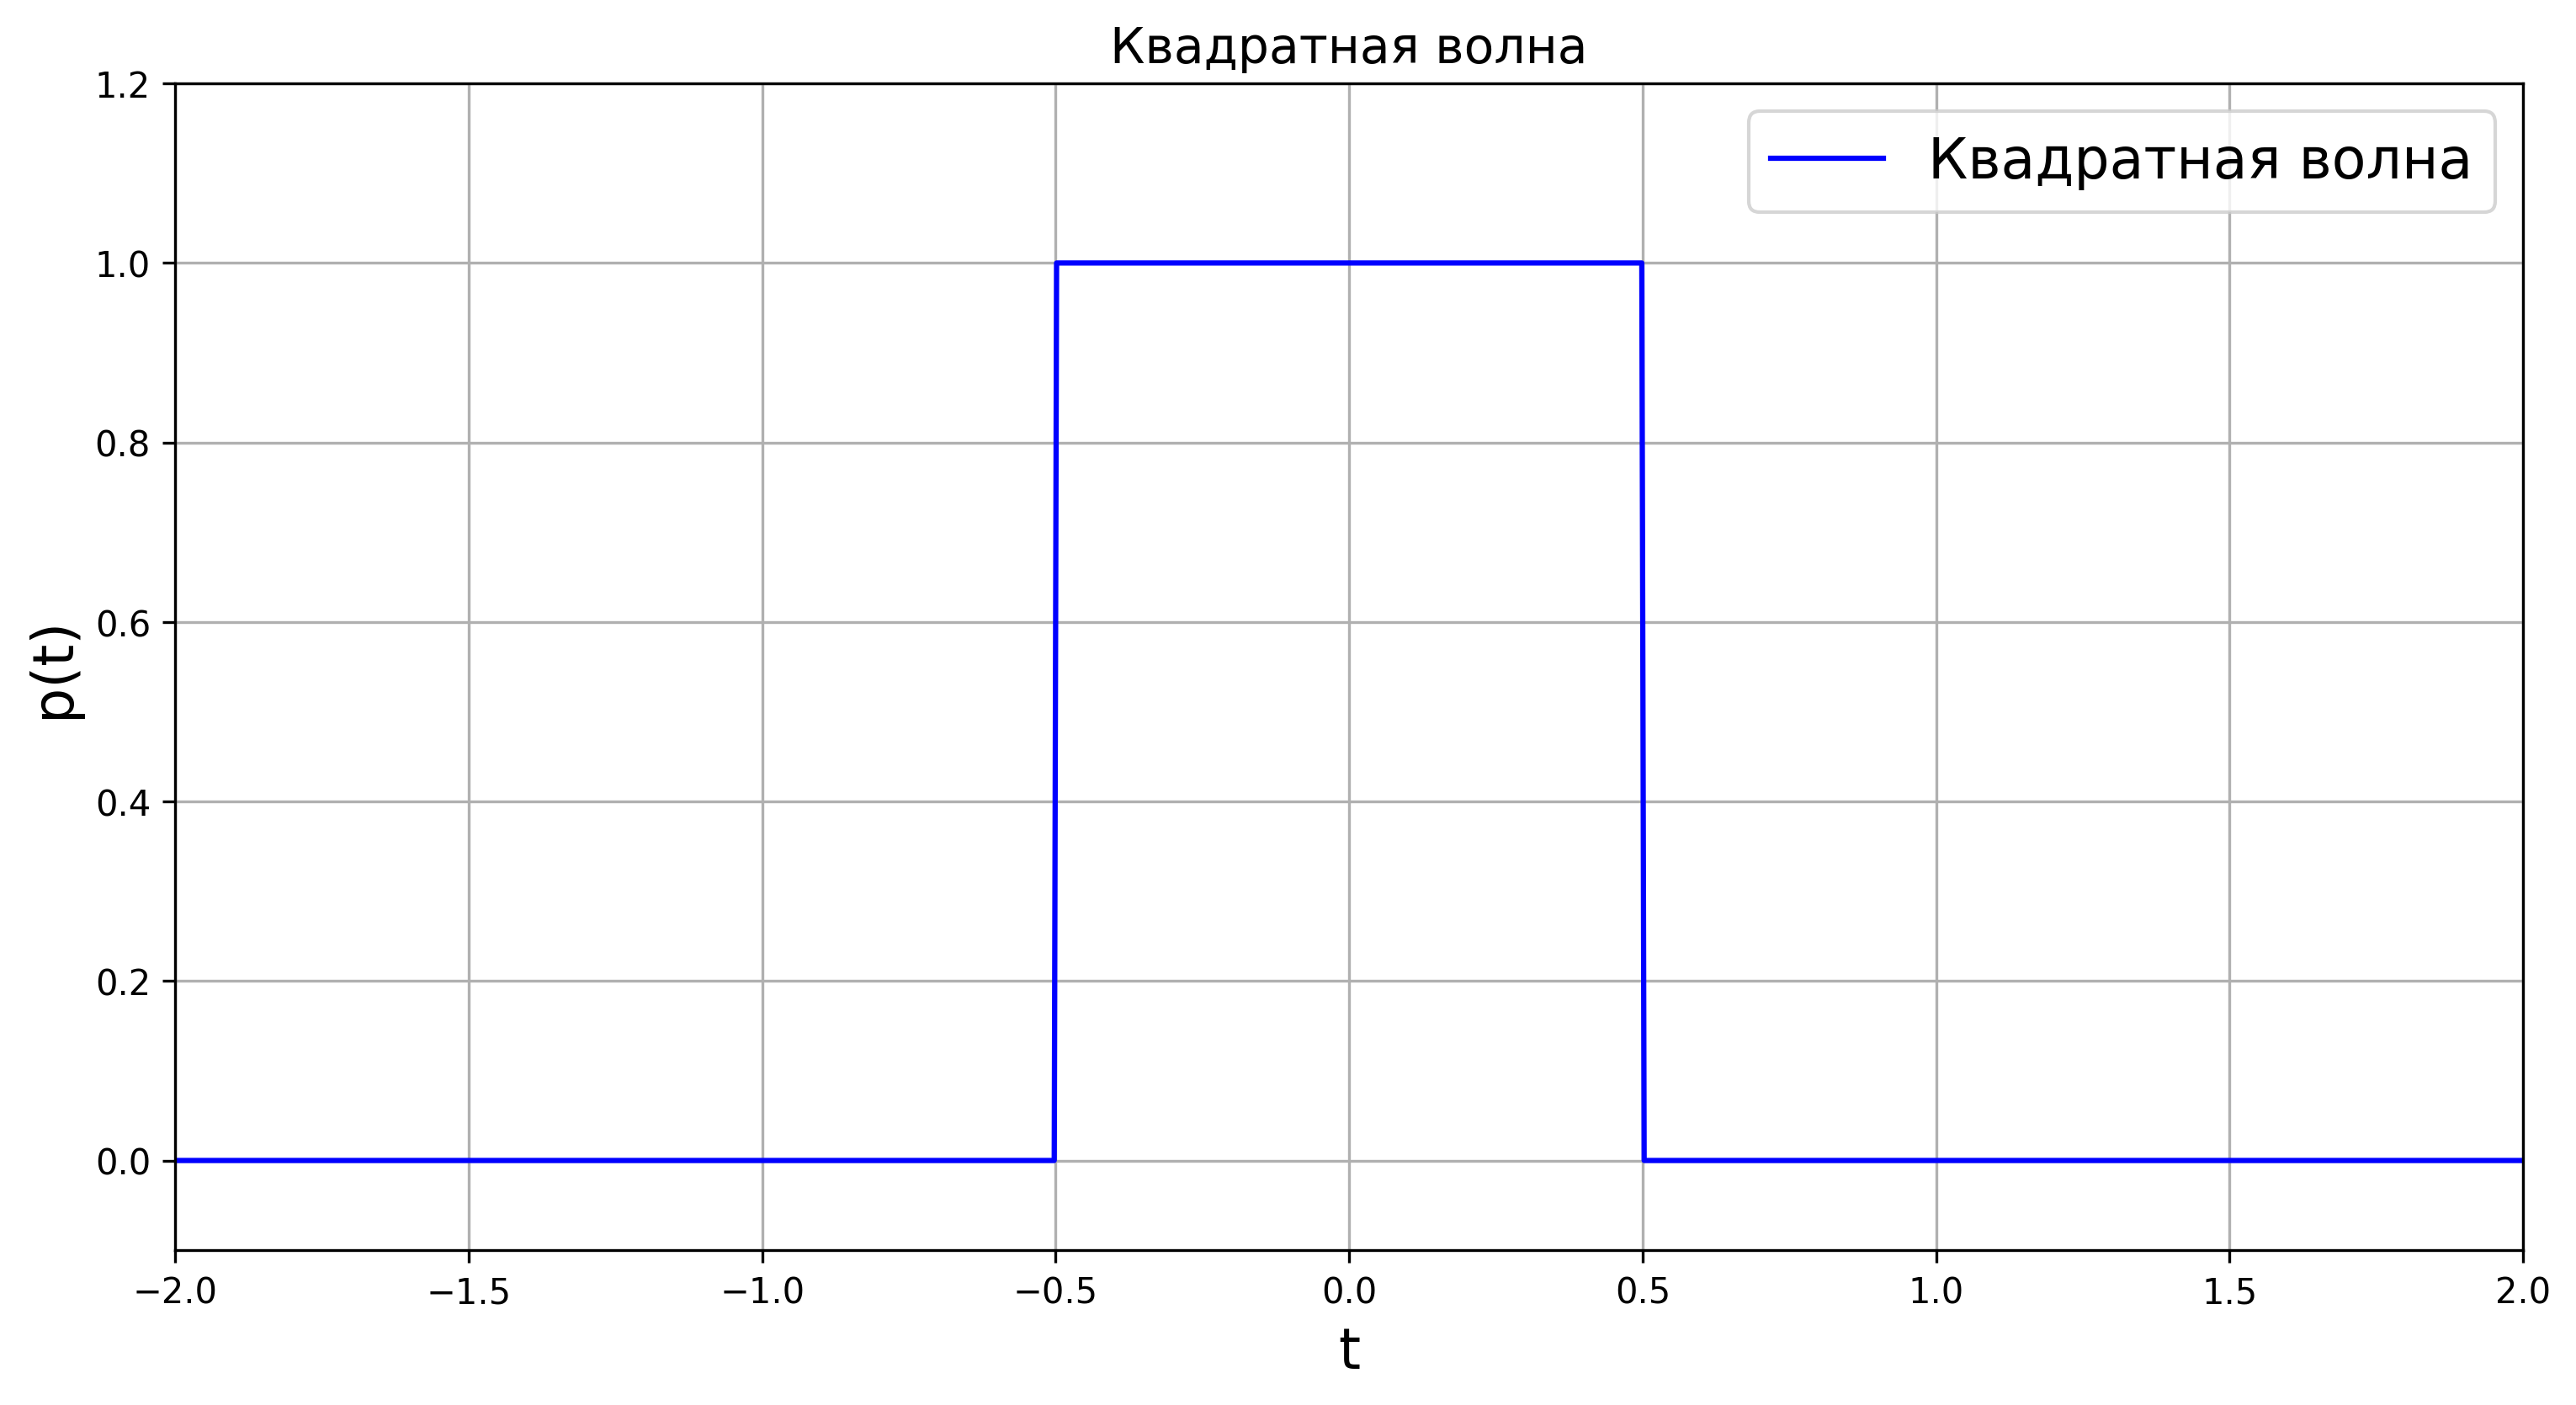
\includegraphics[width=0.85\textwidth, keepaspectratio]{images/pi_true.png}
    \caption{Фурье-образы двух методов при $b_1 = 1$}
\end{figure}

Вычислим её Фурье-образ
\[
\hat{\Pi}(\nu) = \int^{+\inf}_{-\inf}\Pi(t)e^{-2\pi i\nu t}dt = \int^{1/2}_{-1/2}e^{-2\pi i\nu t}dt = -\frac{1}{2\pi i\nu}e^{-2\pi i\nu t}|^{1/2}_{-1/2}
\]
\[
= -\frac{1}{2\pi i\nu}(e^{-\pi i\nu} - e^{\pi i\nu})
\]
\begin{figure}[H]
    \centering
    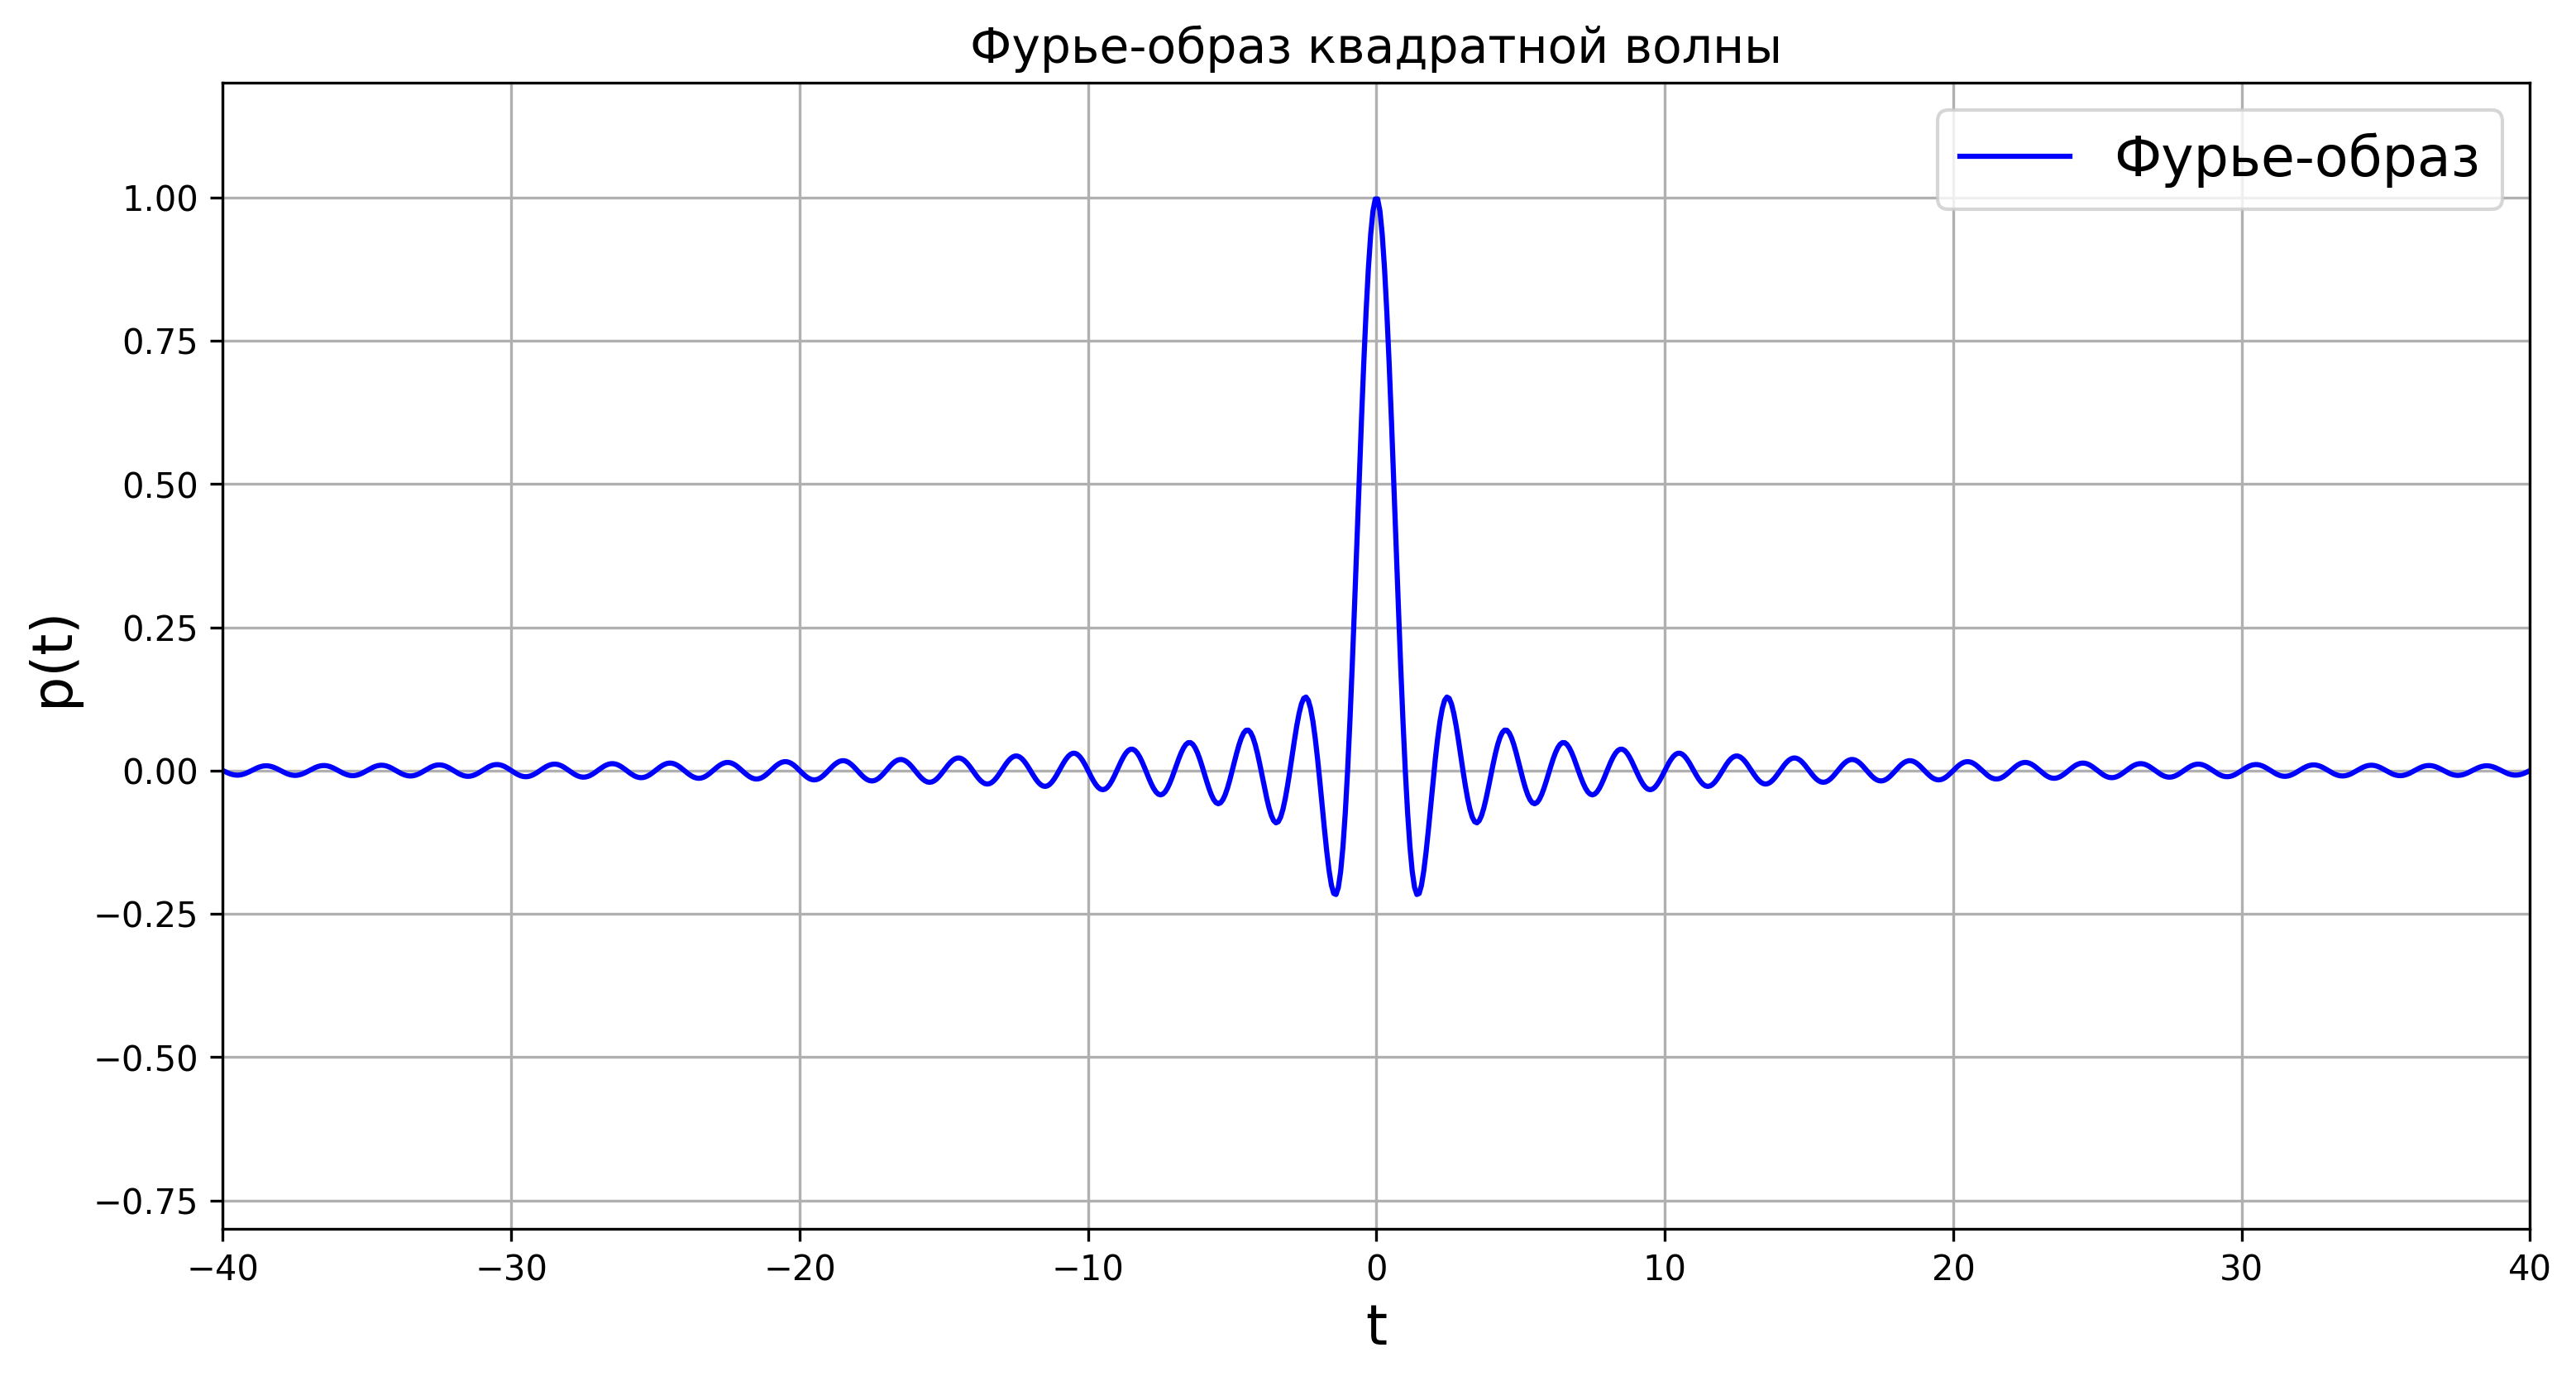
\includegraphics[width=0.95\textwidth, keepaspectratio]{images/fur_pi.png}
    \caption{Фурье-образы двух методов при $b_1 = 1$}
\end{figure}
\subsection{Численное интегрирование}
При рассмотрении различных параметров составления преобразования Фурье видно, что при слишком малом периоде дискритизации, но достаточно малом шаге интегрирования
функция восстанавливается достаточно близкой, но виден эффект Гиббса. При достаточно большом периоде и малых шагах функция восстанавливается идеально. При слишком большом шаге дискретизации
хоть частот, хоть времени функция восстанавливается неверно, она больше оригинальной, может появиться период как на графике функции, так и на графике образа.
\newpage
\subsection*{Комбинация 1: $T=4$, $V=100$, $dt=0.01$, $dv=0.1$}

\begin{figure}[H]
    \centering
    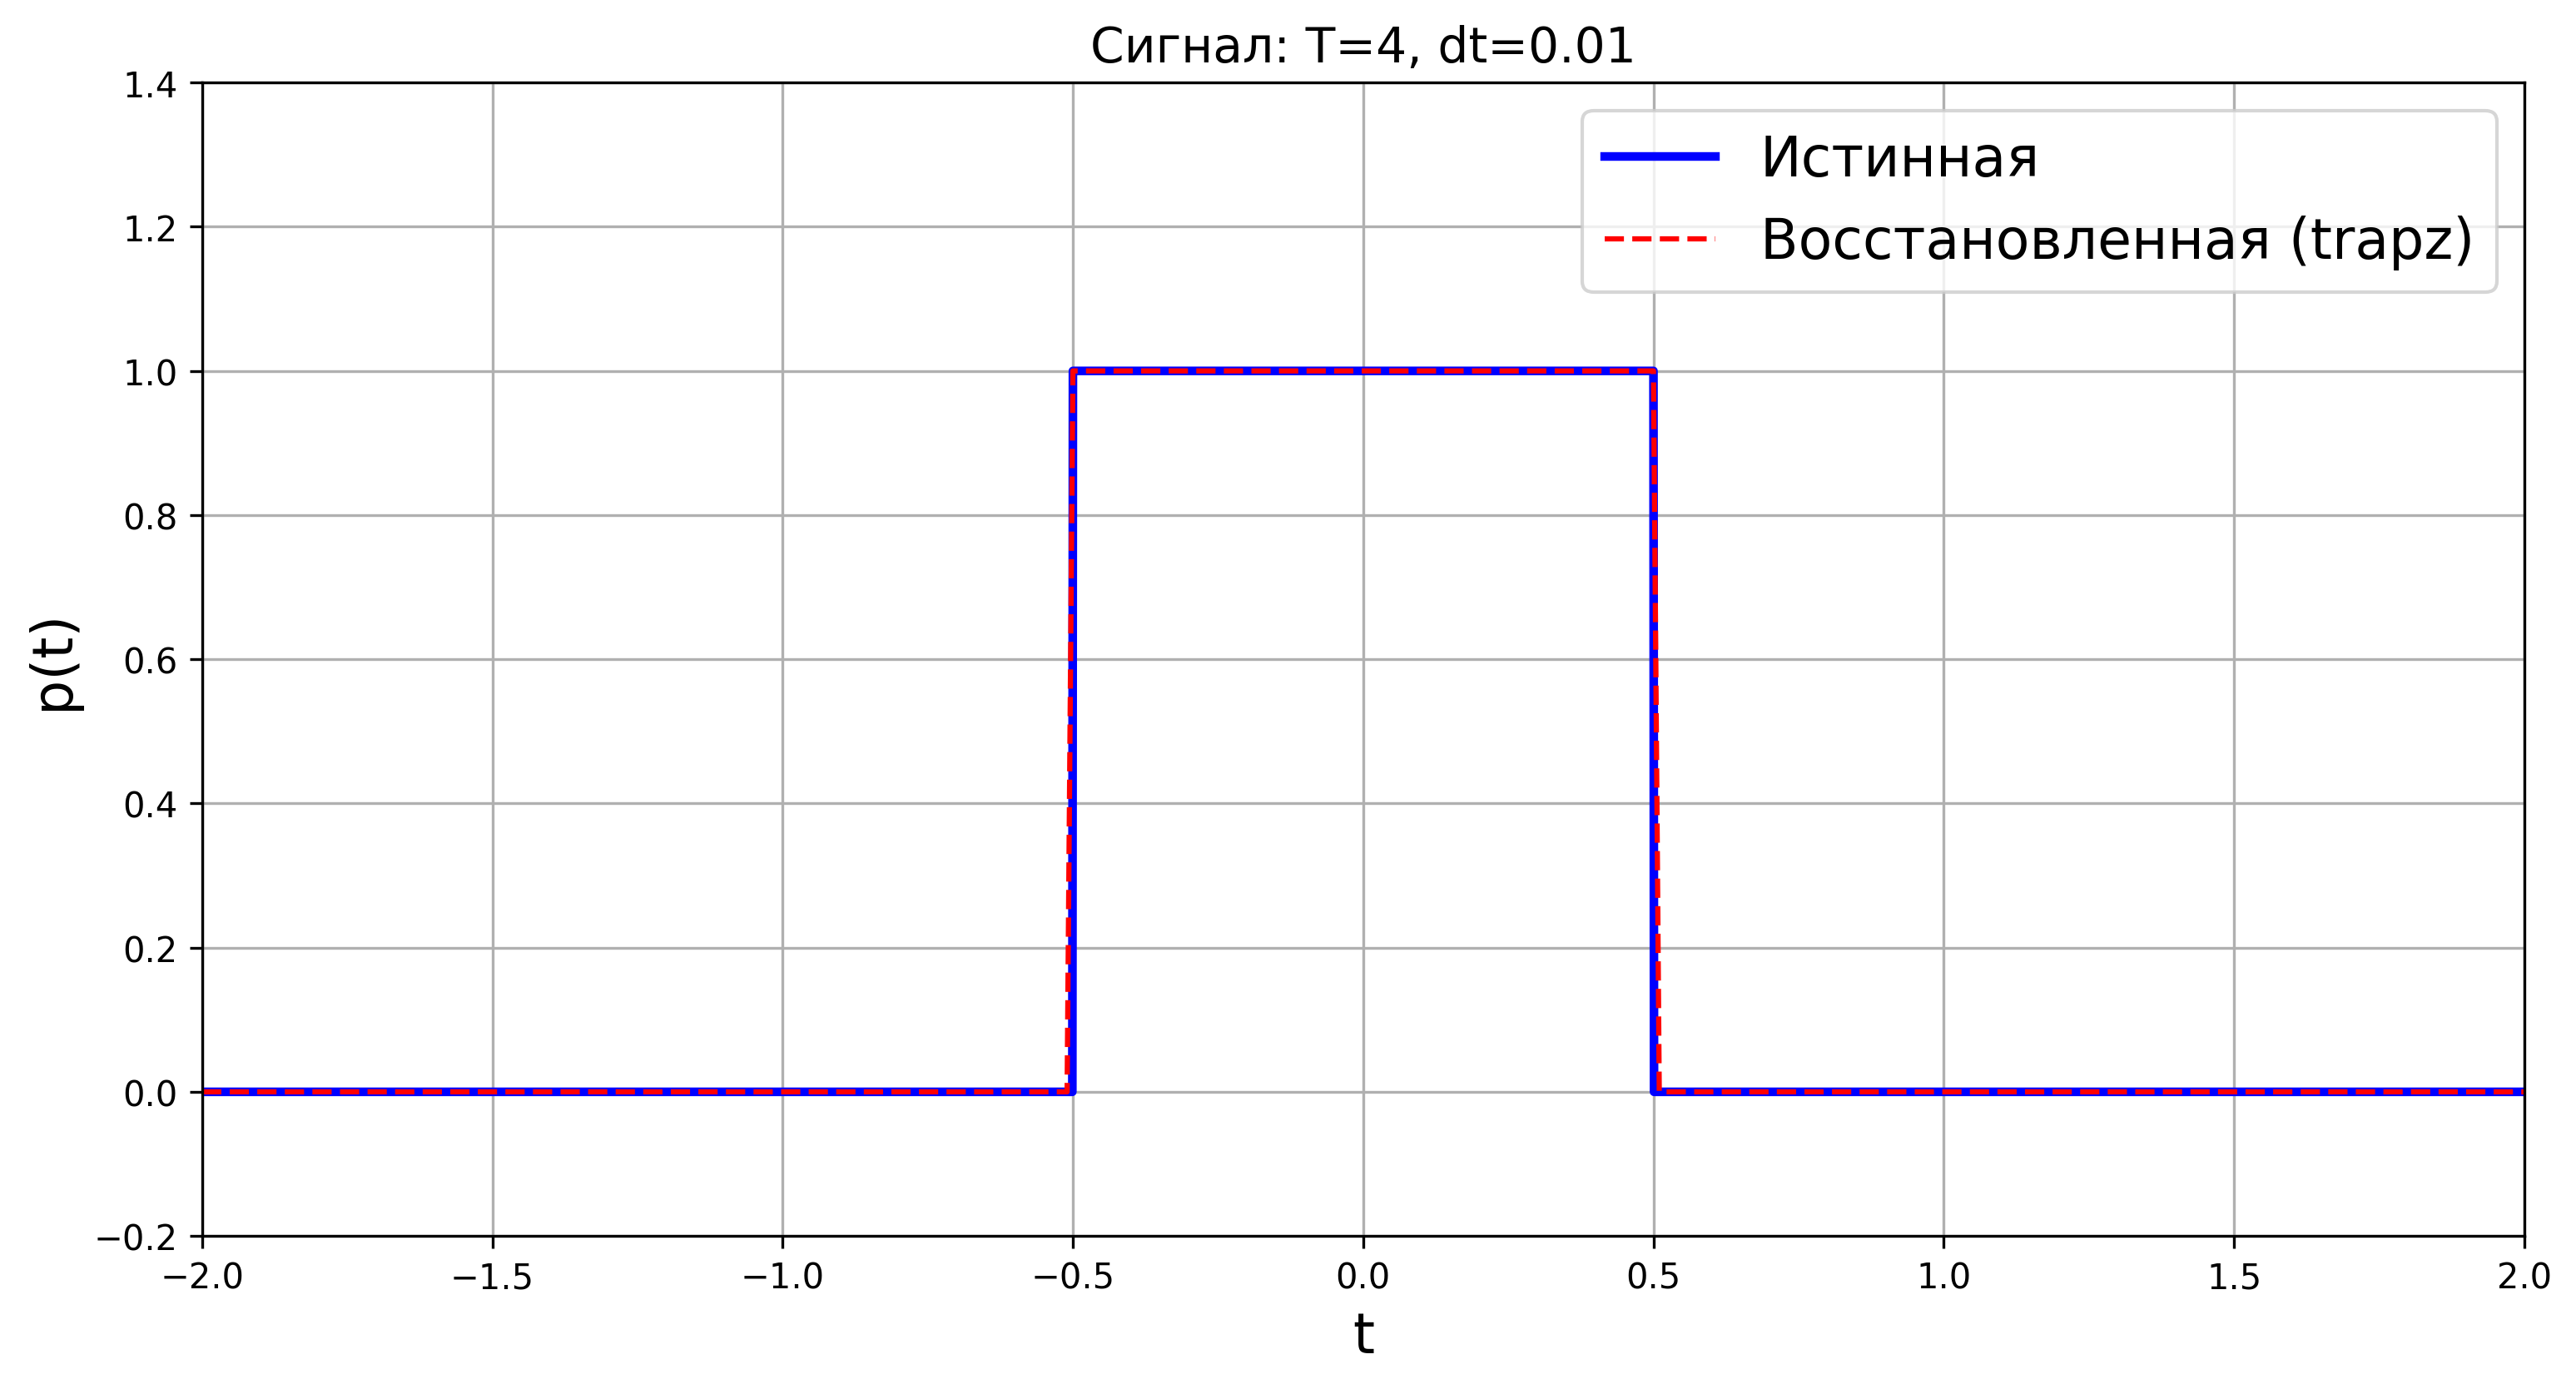
\includegraphics[width=0.95\textwidth]{images/T4_V100_dt0.010_dv0.100_signal.png}
    \caption{Восстановление сигнала: $T=4$, $dt=0.01$.}
\end{figure}

\begin{figure}[H]
    \centering
    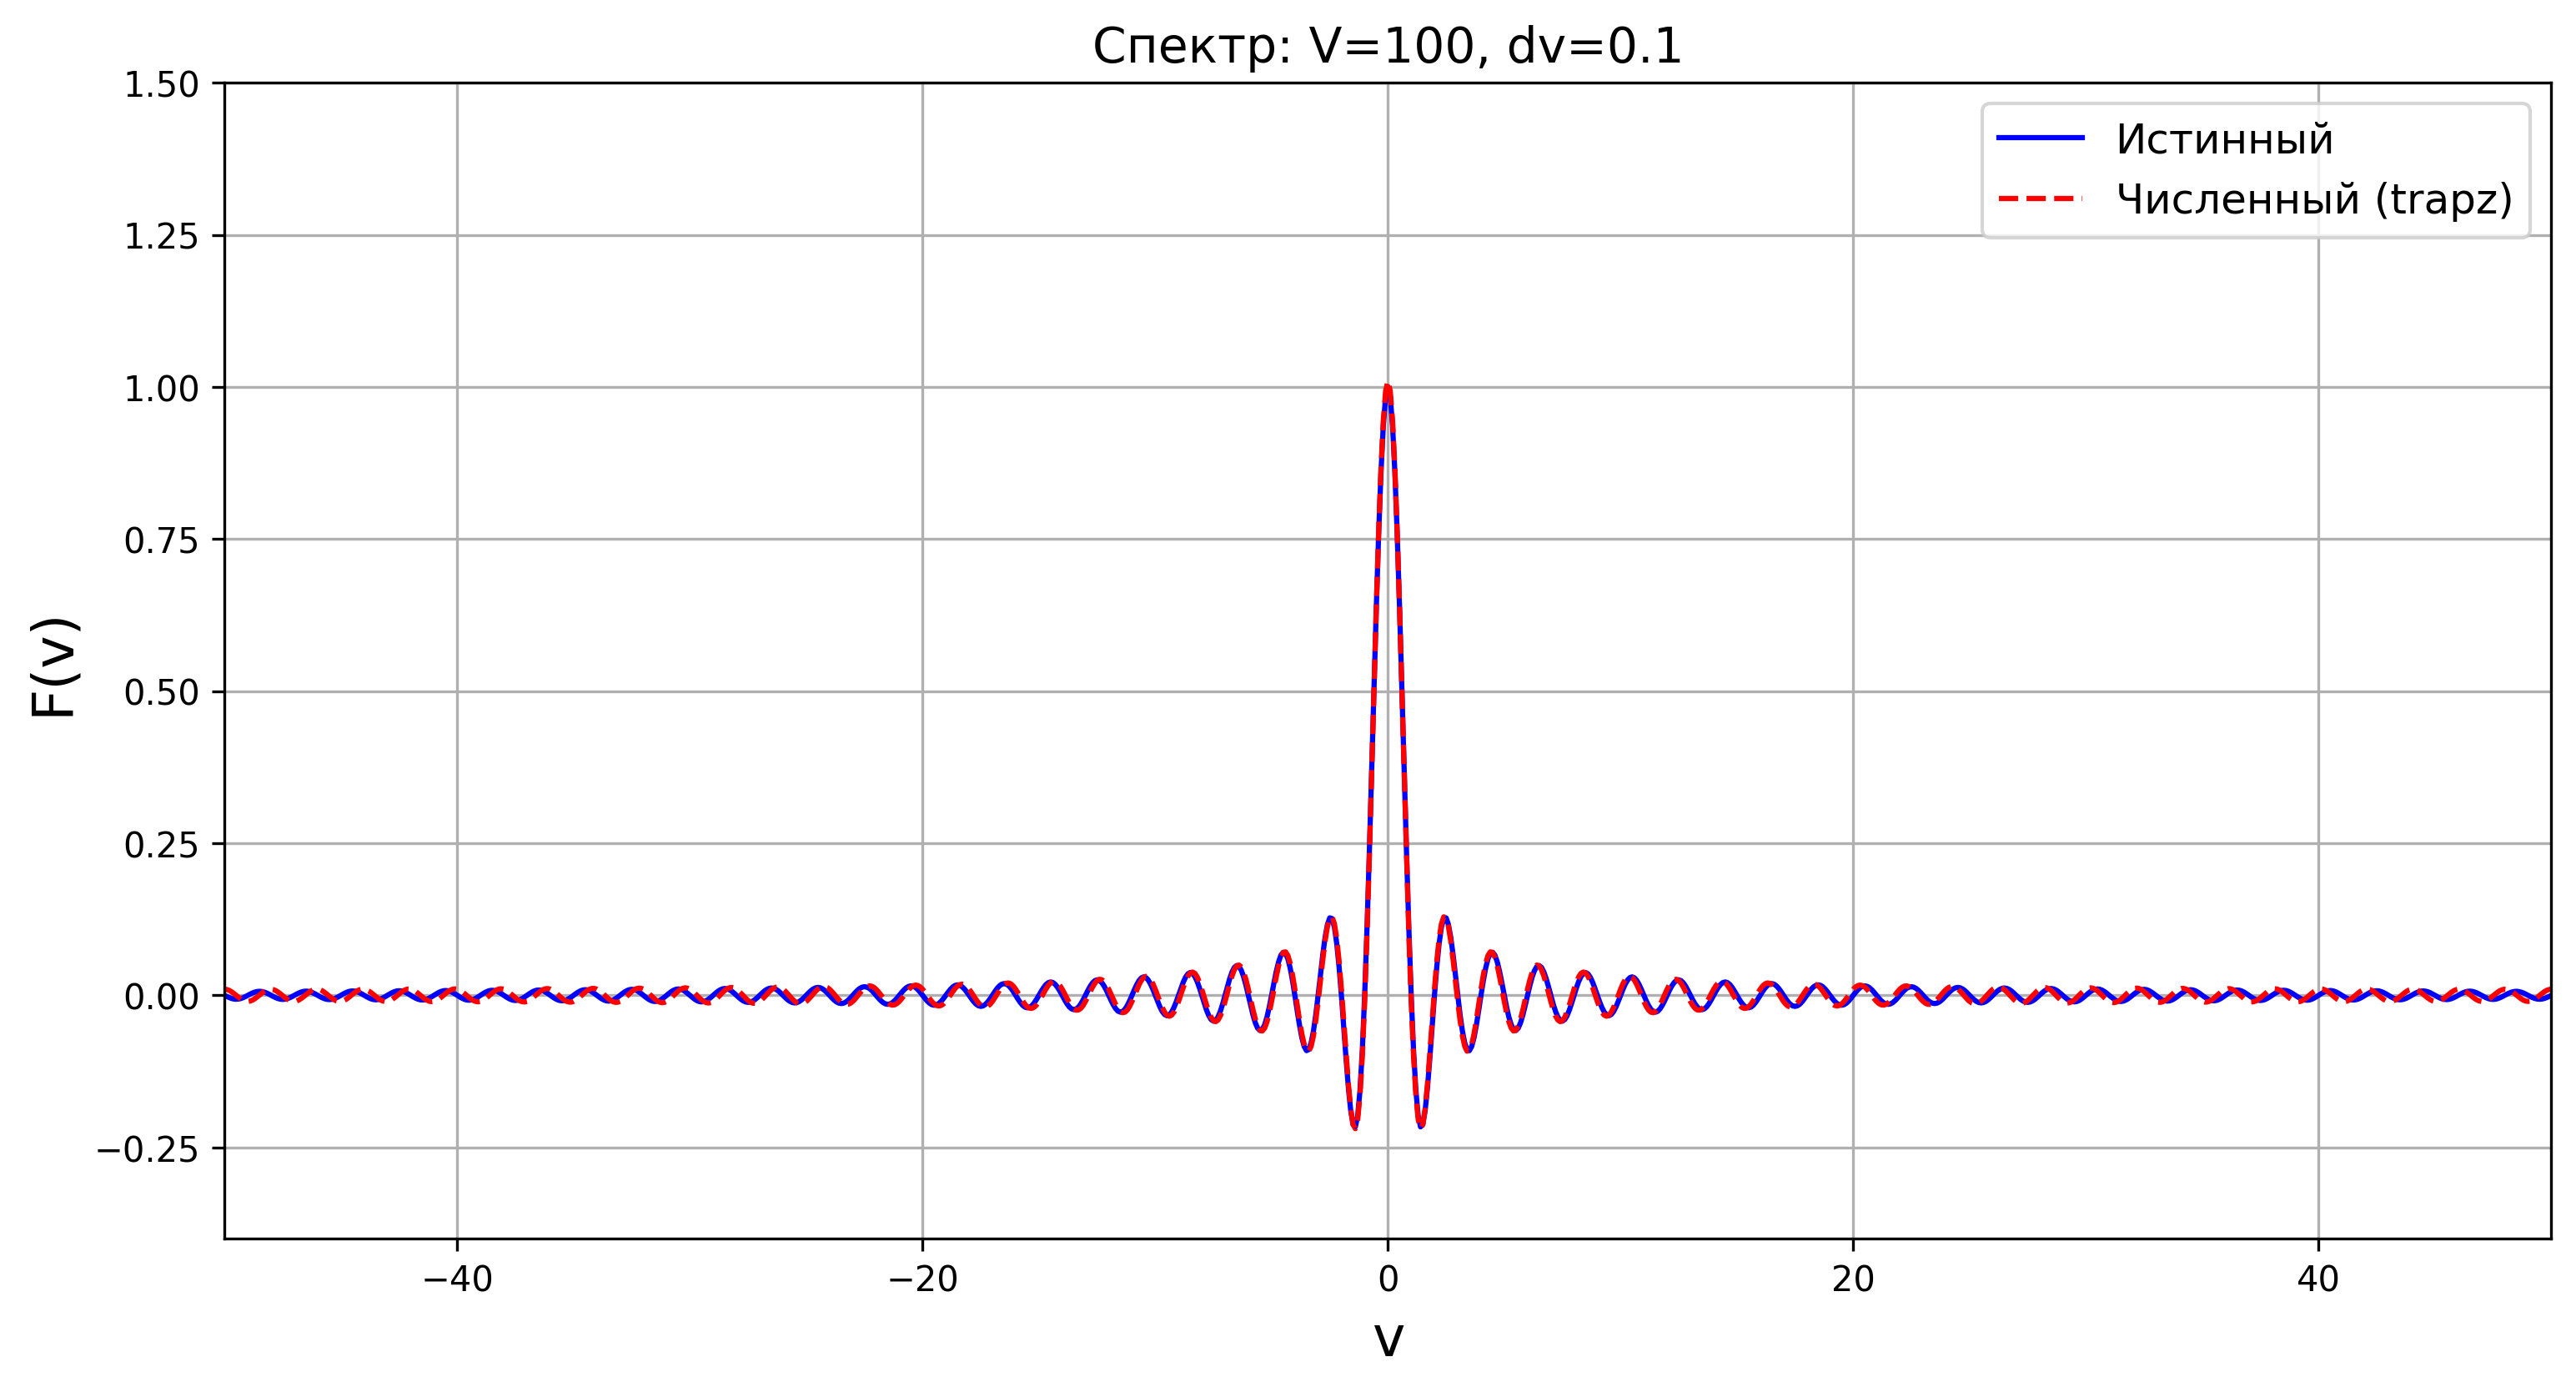
\includegraphics[width=0.95\textwidth]{images/T4_V100_dt0.010_dv0.100_spectrum.png}
    \caption{Сравнение спектров: $V=100$, $dv=0.1$.}
\end{figure}

\newpage
\subsection*{Комбинация 2: $T=15$, $V=100$, $dt=0.01$, $dv=0.1$}

\begin{figure}[H]
    \centering
    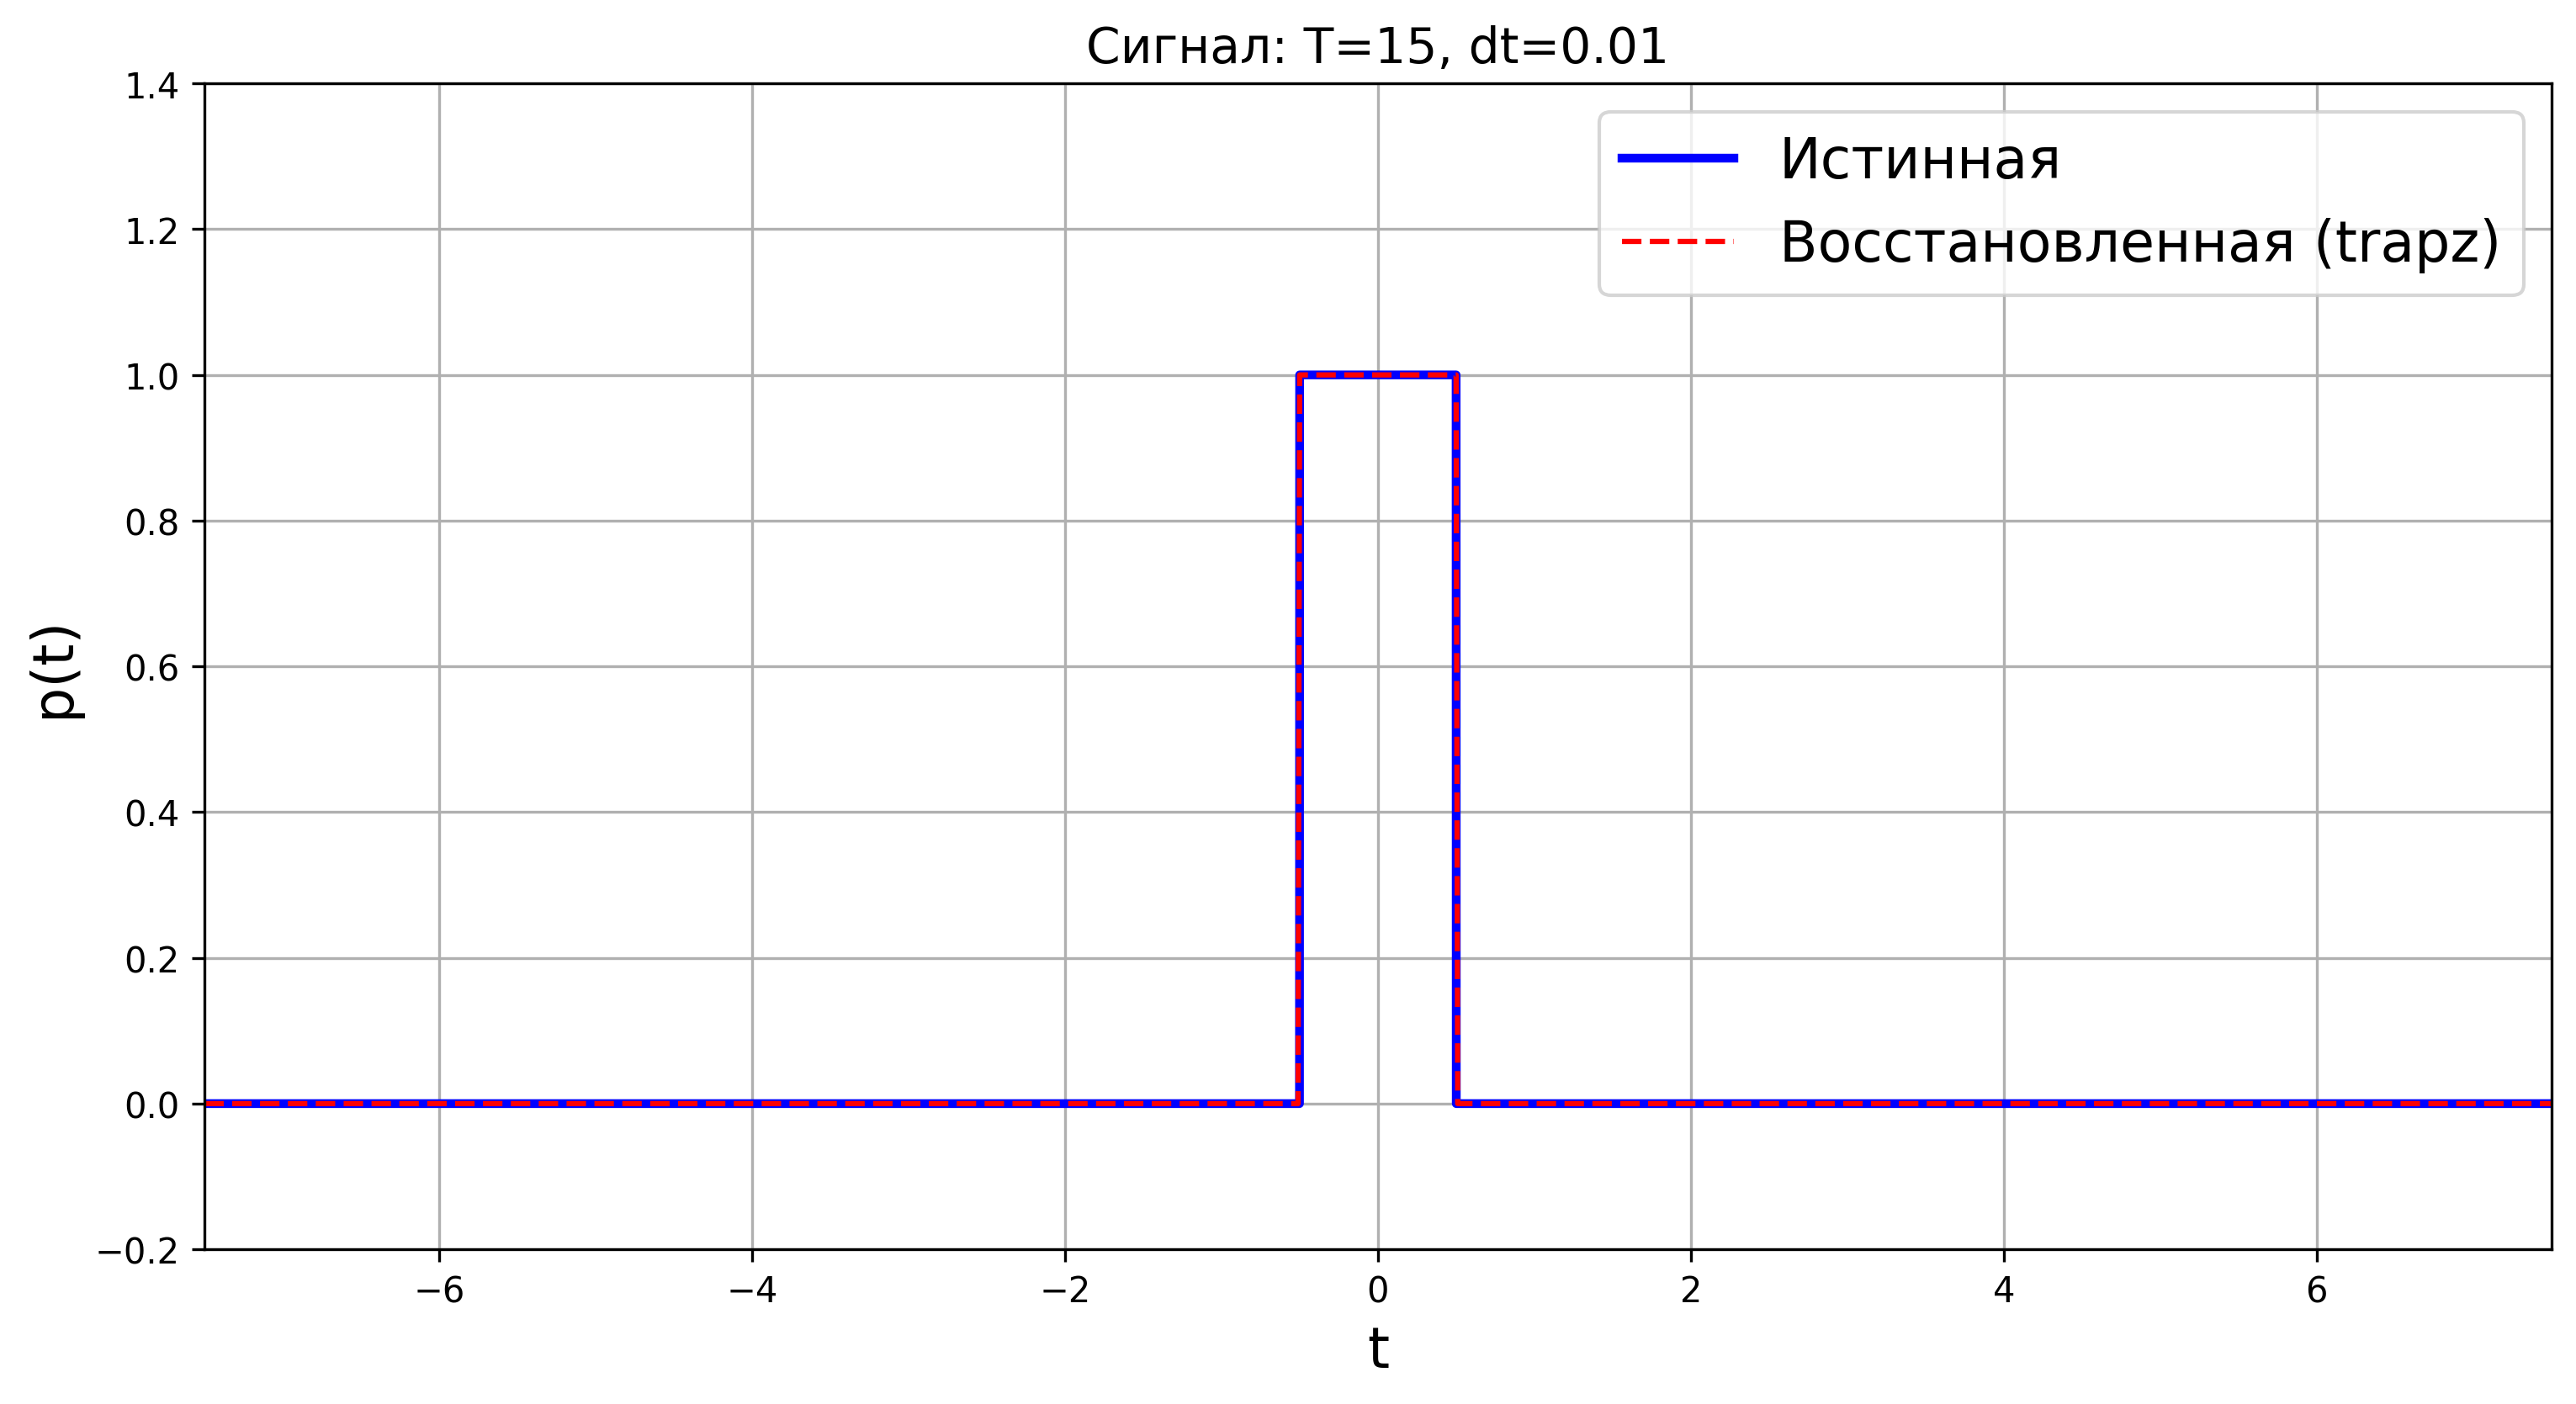
\includegraphics[width=0.95\textwidth]{images/T15_V100_dt0.010_dv0.100_signal.png}
    \caption{Восстановление сигнала: $T=15$, $dt=0.01$.}
\end{figure}

\begin{figure}[H]
    \centering
    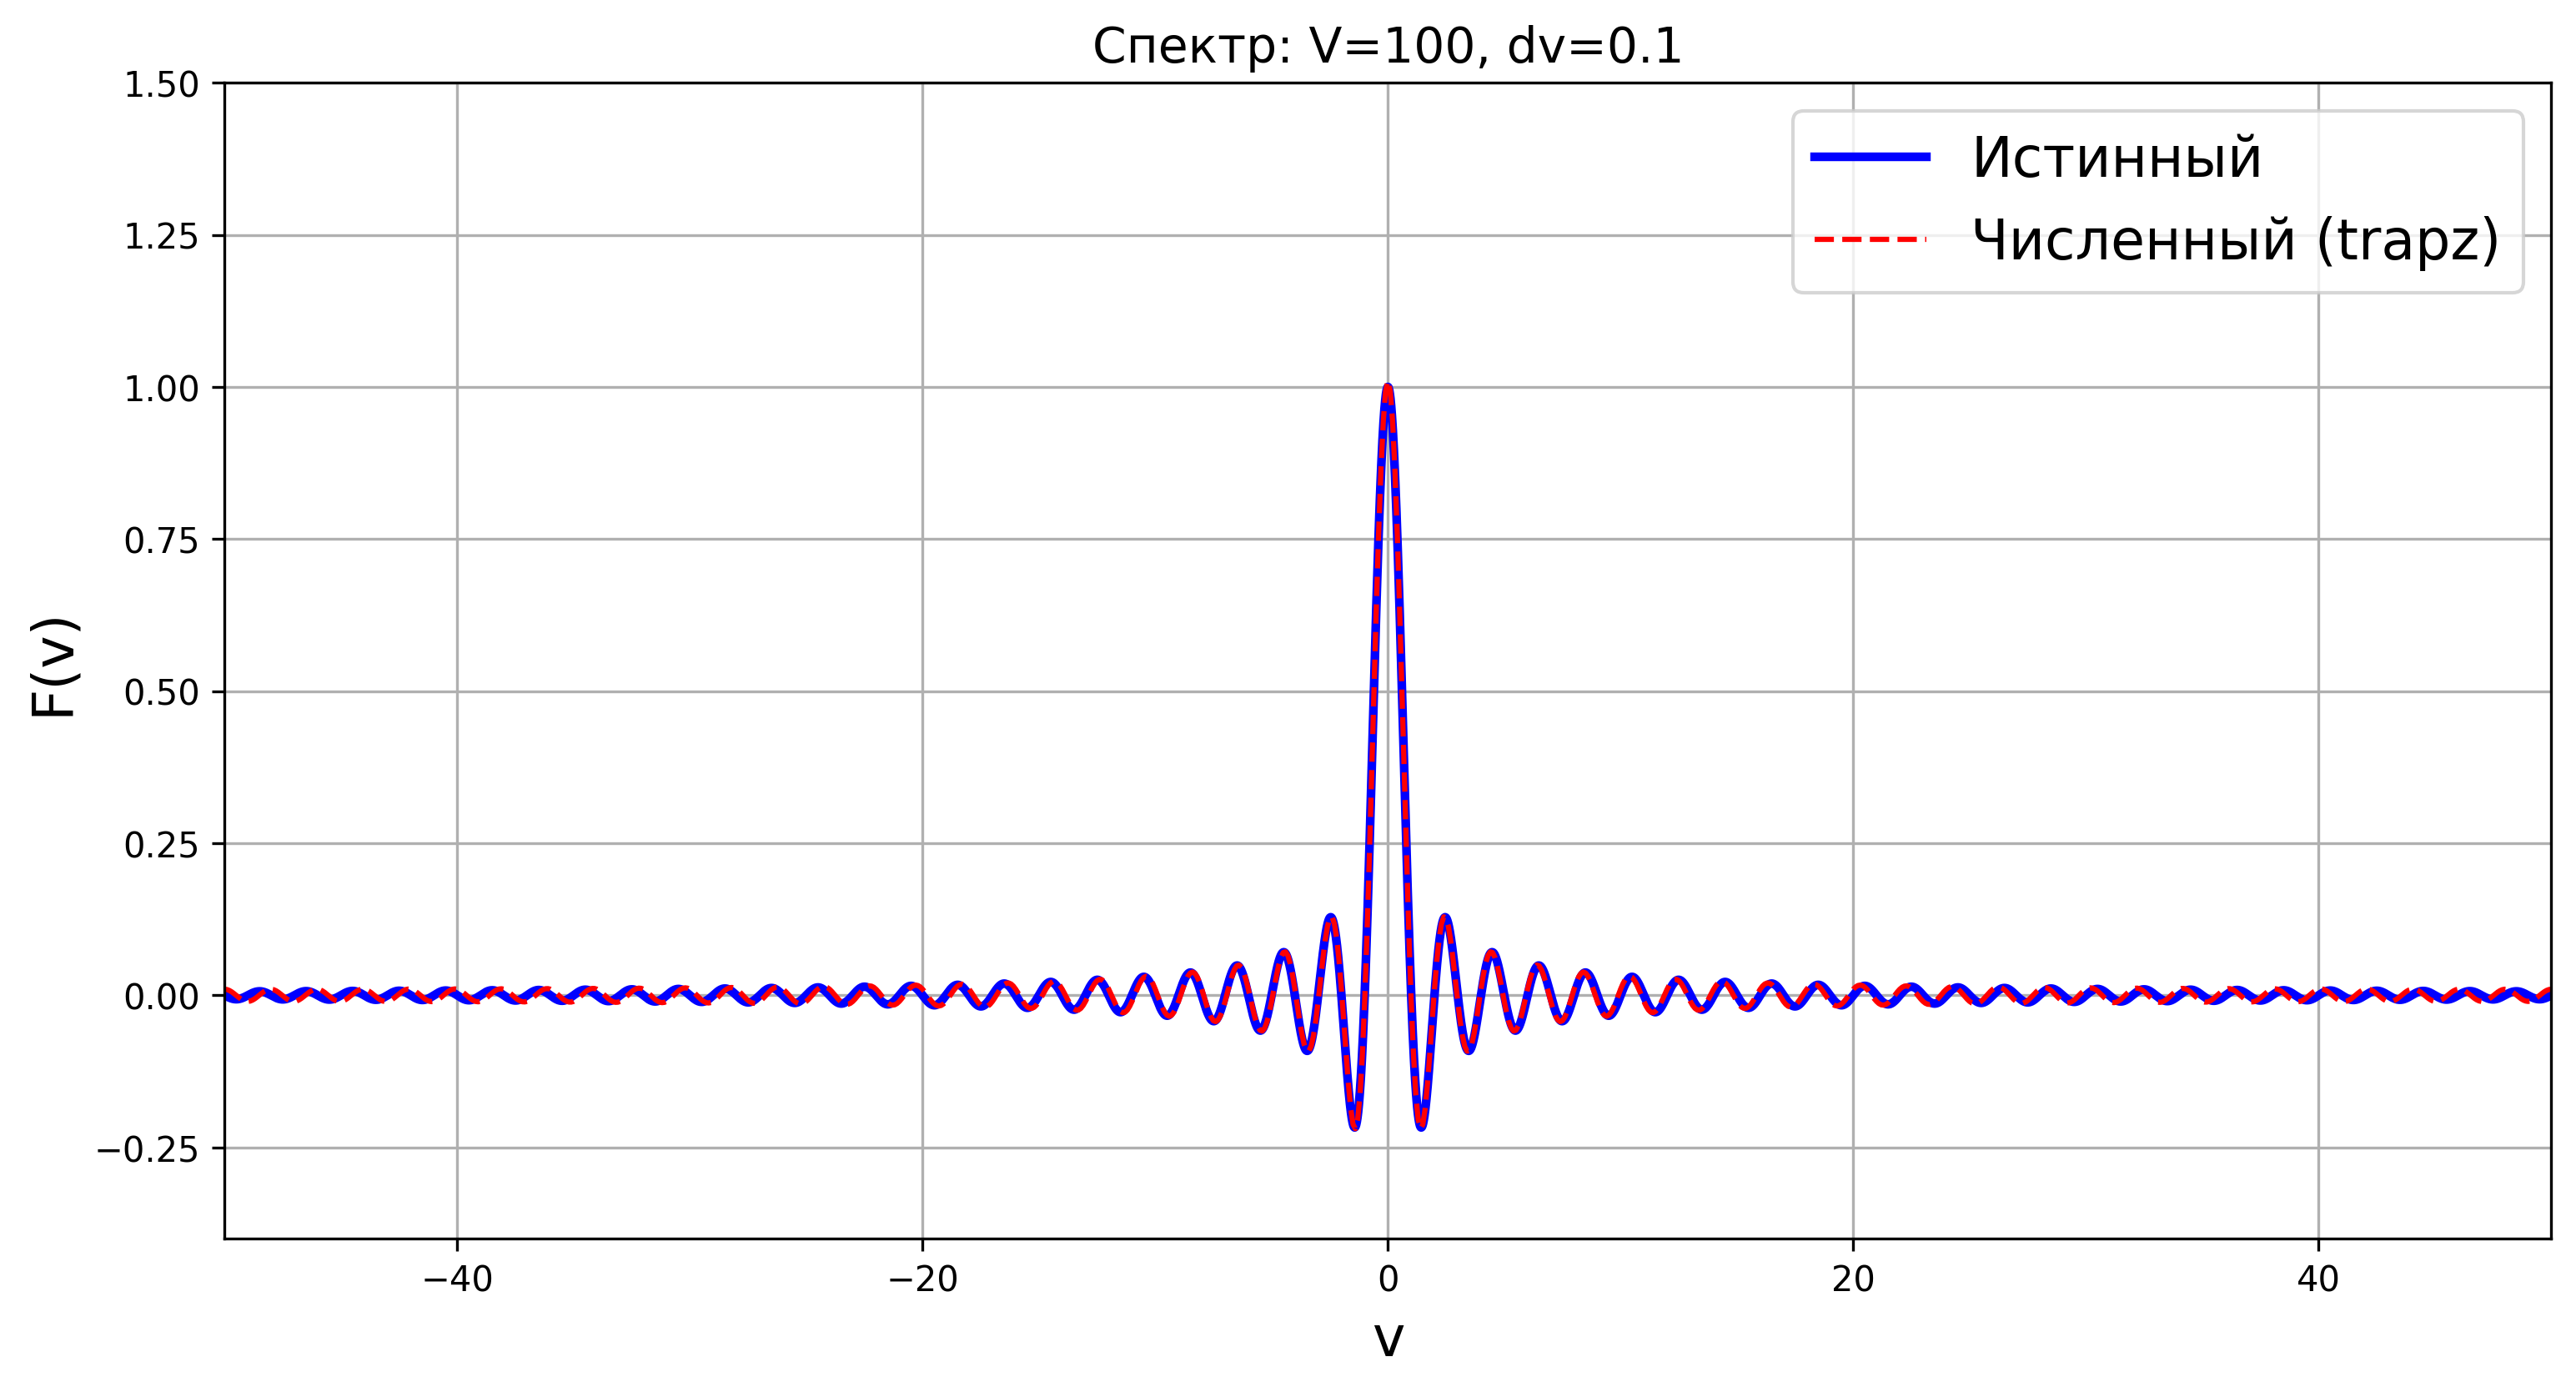
\includegraphics[width=0.95\textwidth]{images/T15_V100_dt0.010_dv0.100_spectrum.png}
    \caption{Сравнение спектров: $V=100$, $dv=0.1$.}
\end{figure}

\newpage
\subsection*{Комбинация 3: $T=4$, $V=200$, $dt=0.01$, $dv=0.1$}

\begin{figure}[H]
    \centering
    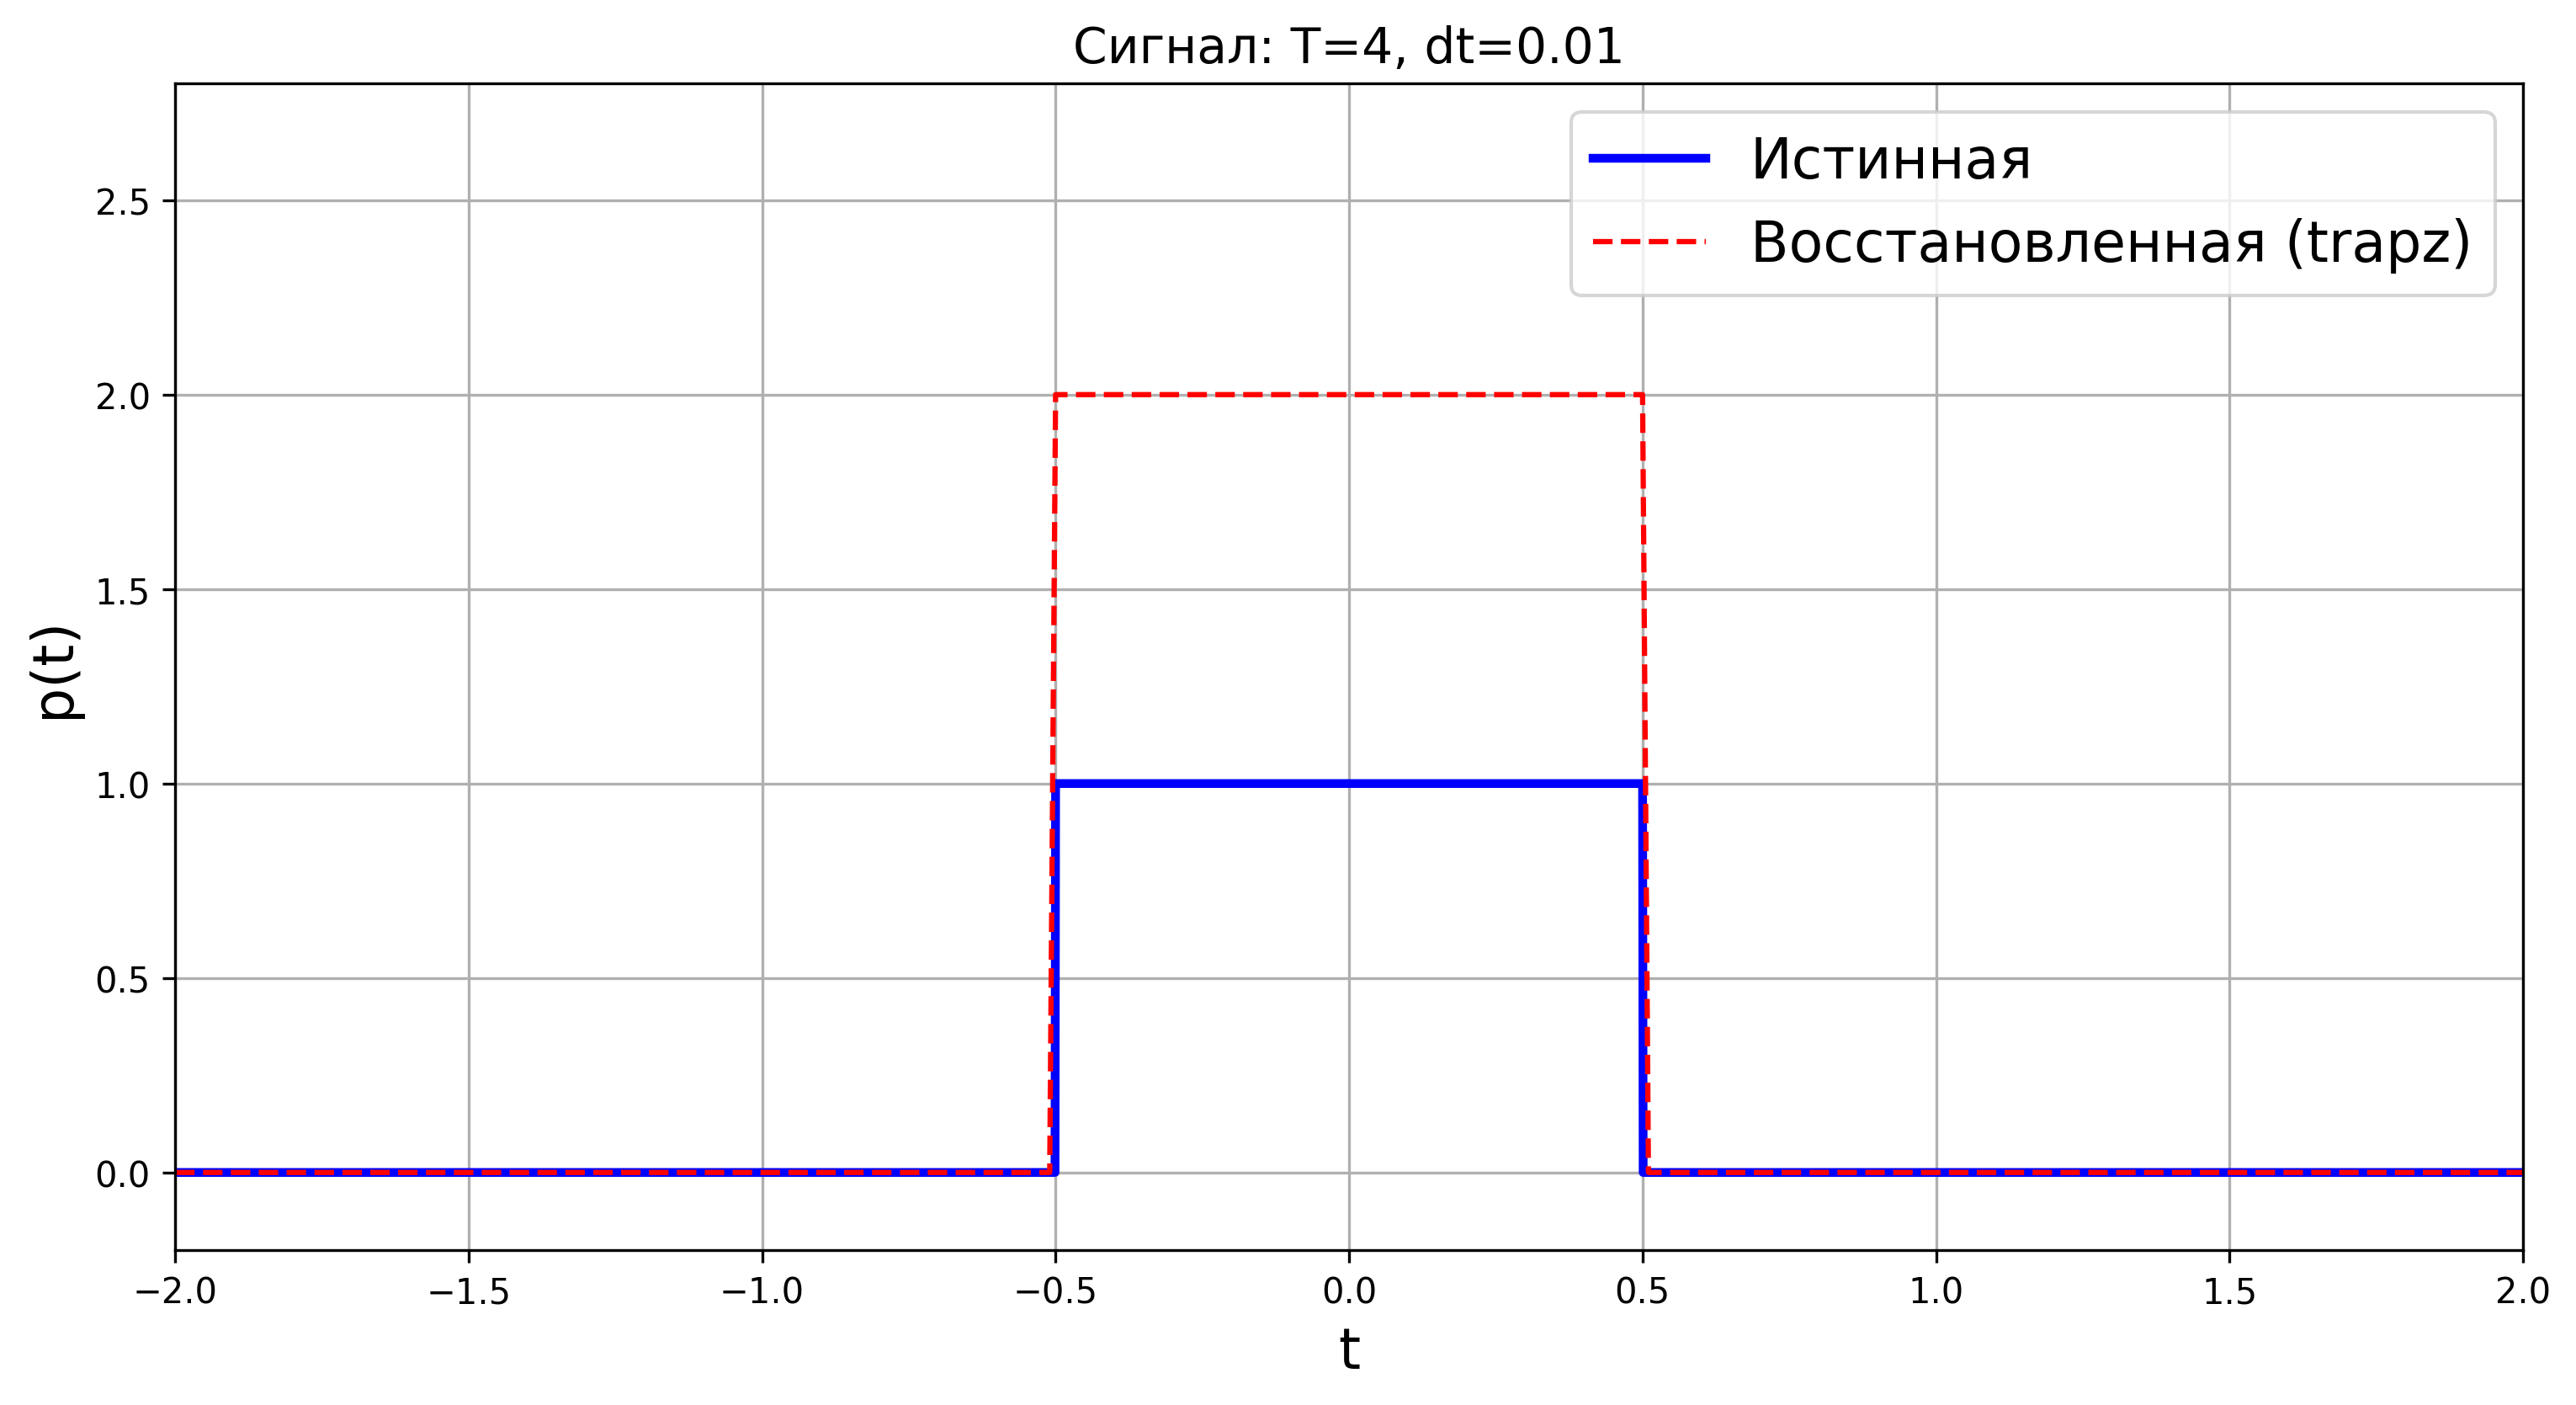
\includegraphics[width=0.95\textwidth]{images/T4_V200_dt0.010_dv0.100_signal.png}
    \caption{Восстановление сигнала: $T=4$, $dt=0.01$.}
\end{figure}

\begin{figure}[H]
    \centering
    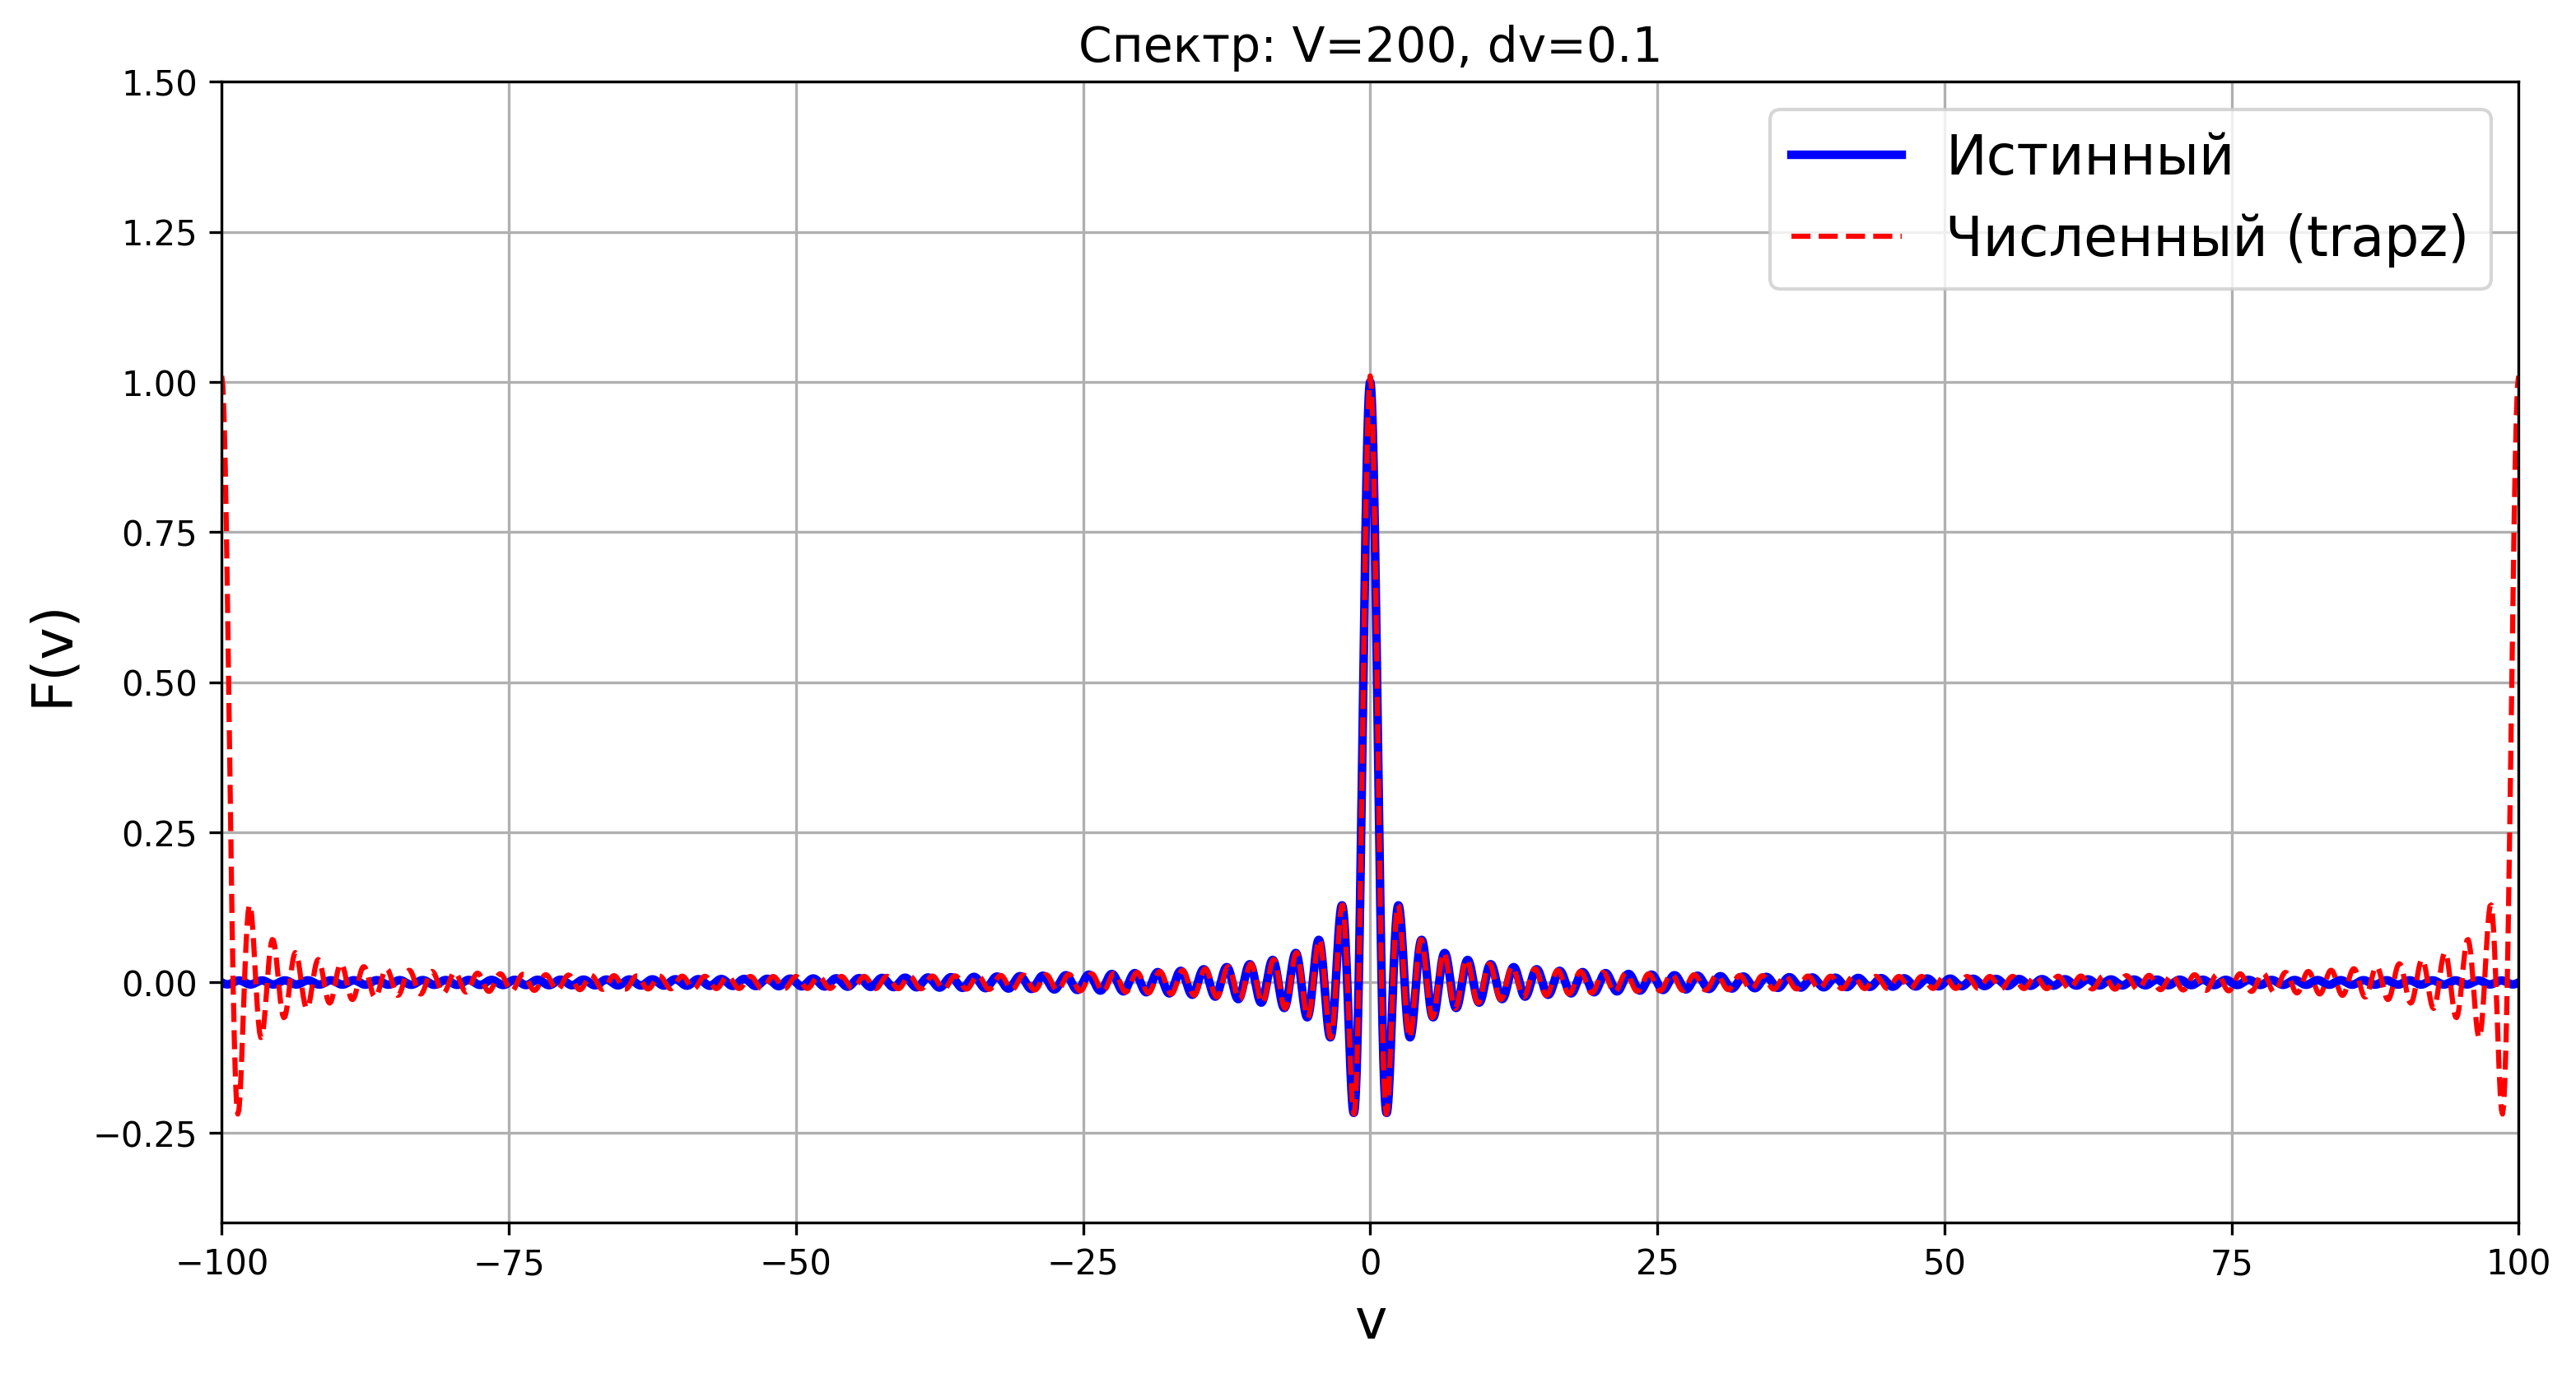
\includegraphics[width=0.95\textwidth]{images/T4_V200_dt0.010_dv0.100_spectrum.png}
    \caption{Сравнение спектров: $V=200$, $dv=0.1$.}
\end{figure}

\newpage
\subsection*{Комбинация 4: $T=4$, $V=100$, $dt=0.1$, $dv=0.1$}

\begin{figure}[H]
    \centering
    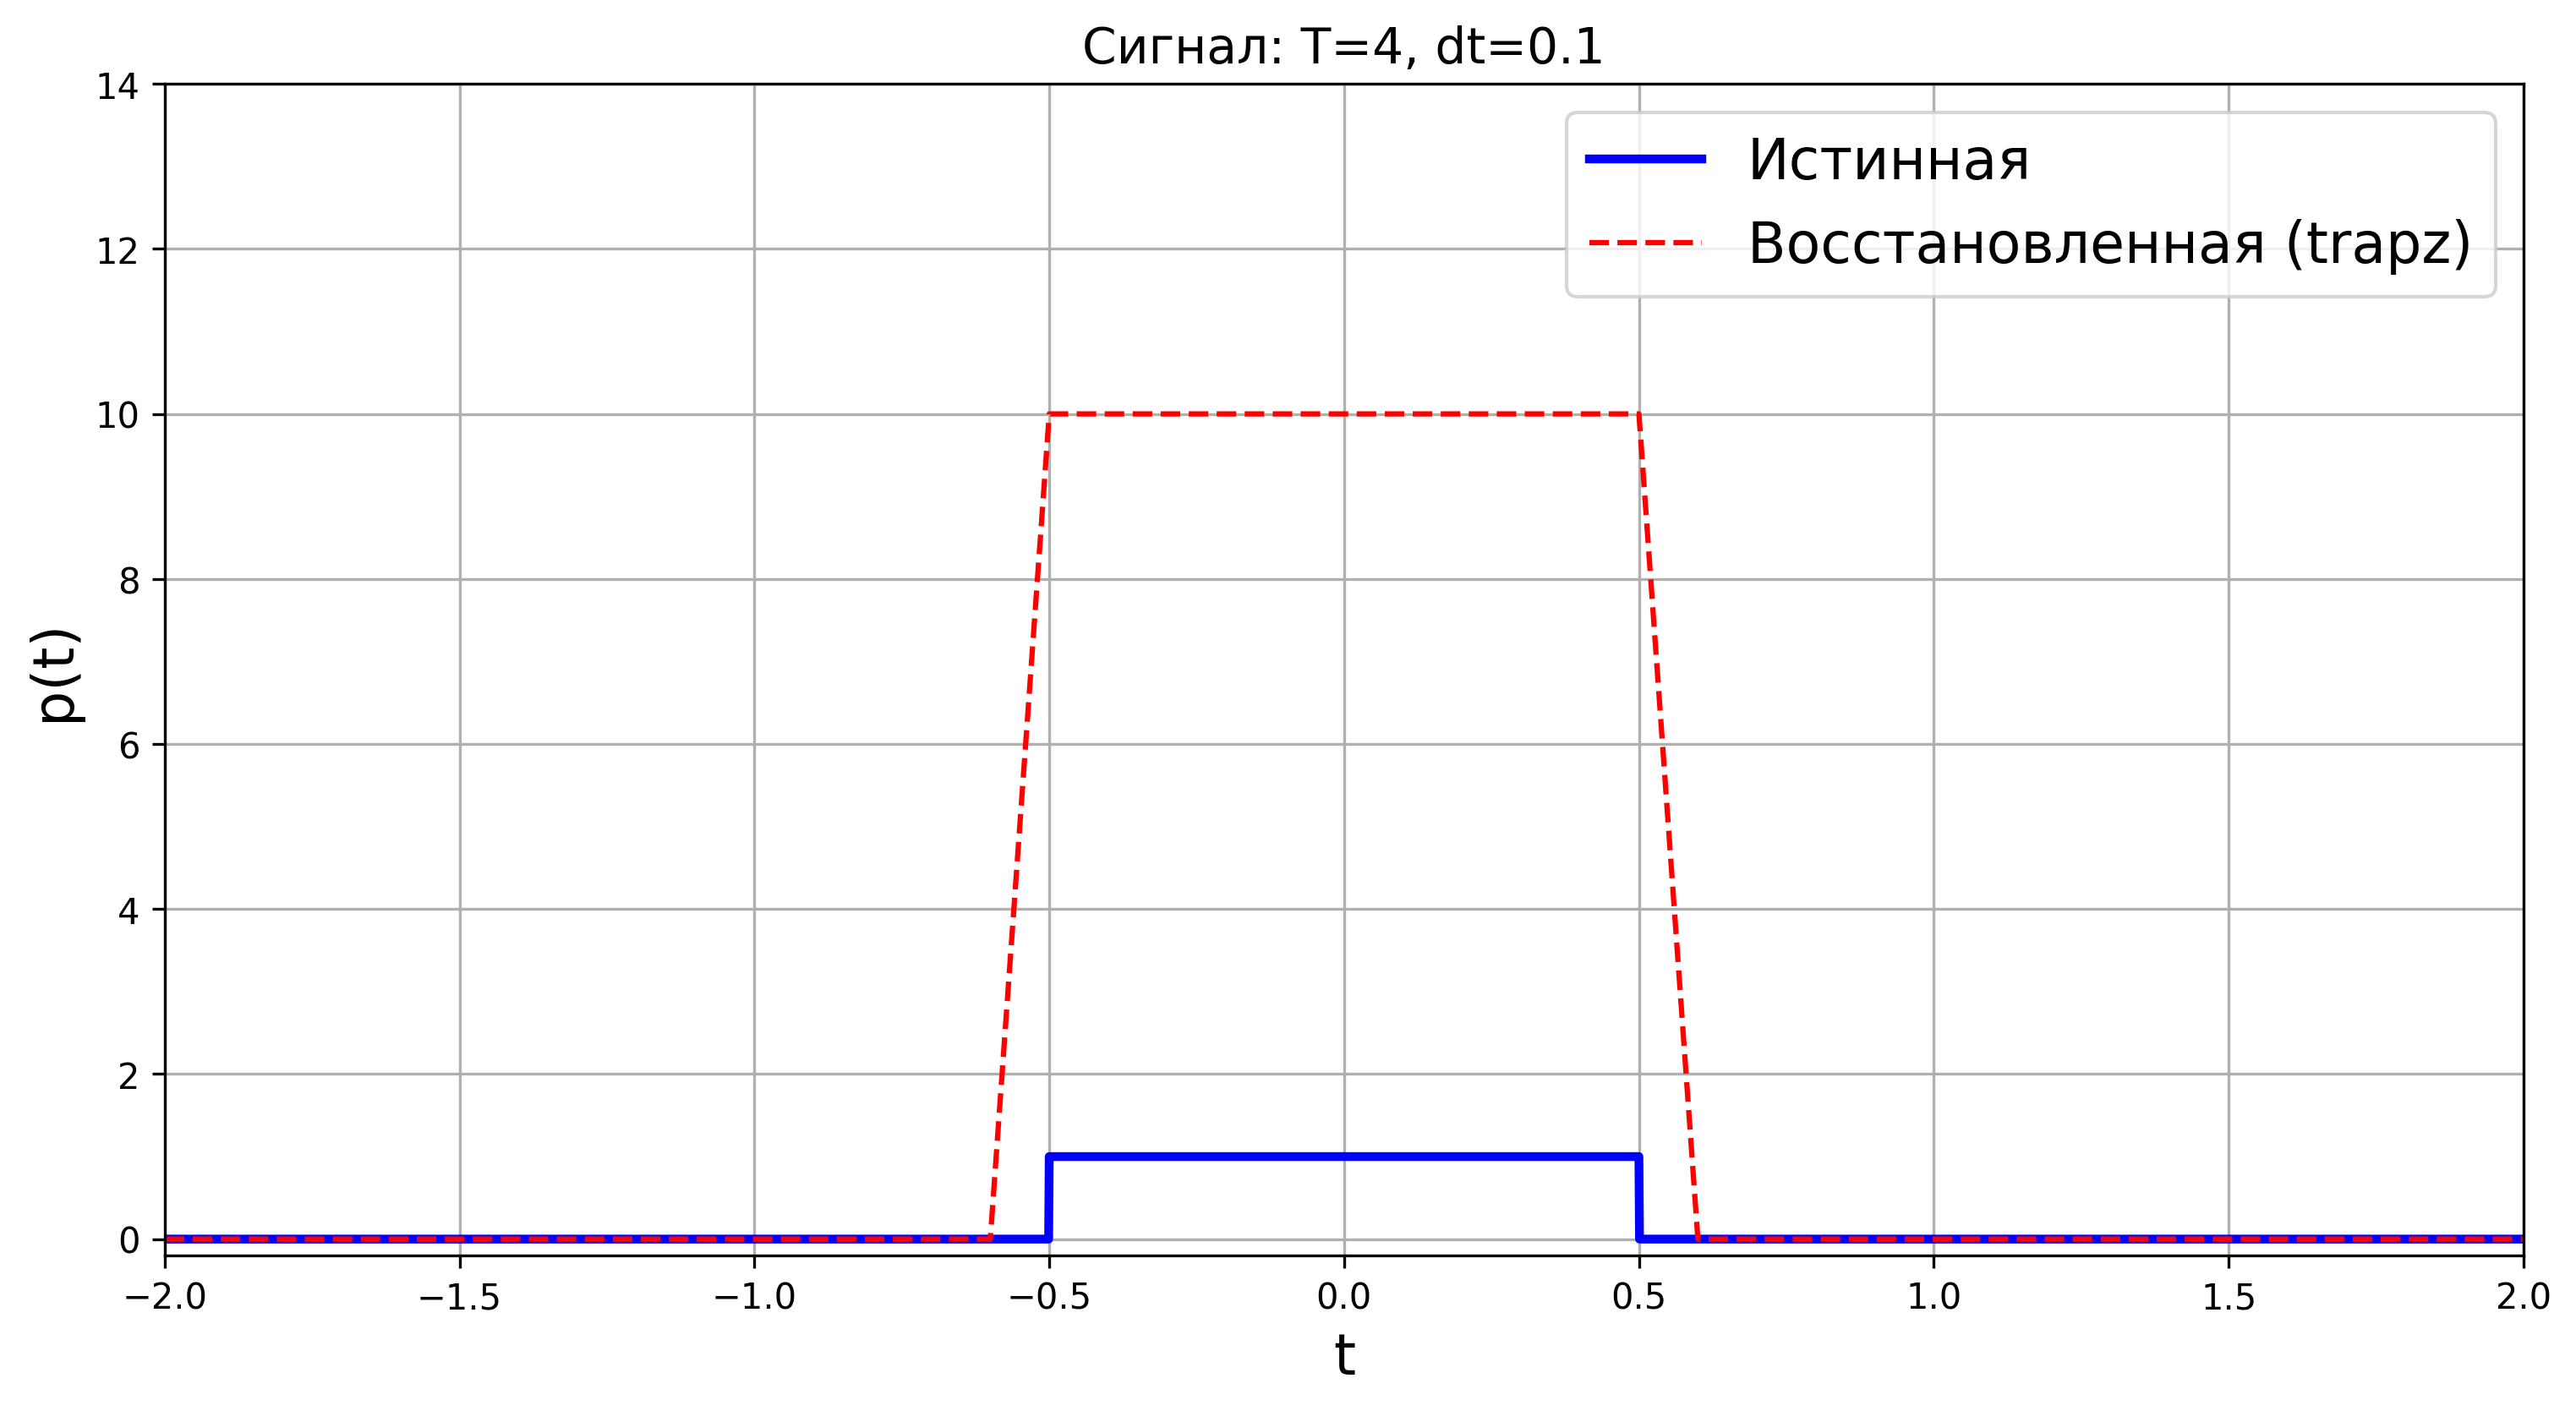
\includegraphics[width=0.95\textwidth]{images/T4_V100_dt0.100_dv0.100_signal.png}
    \caption{Восстановление сигнала: $T=4$, $dt=0.1$.}
\end{figure}

\begin{figure}[H]
    \centering
    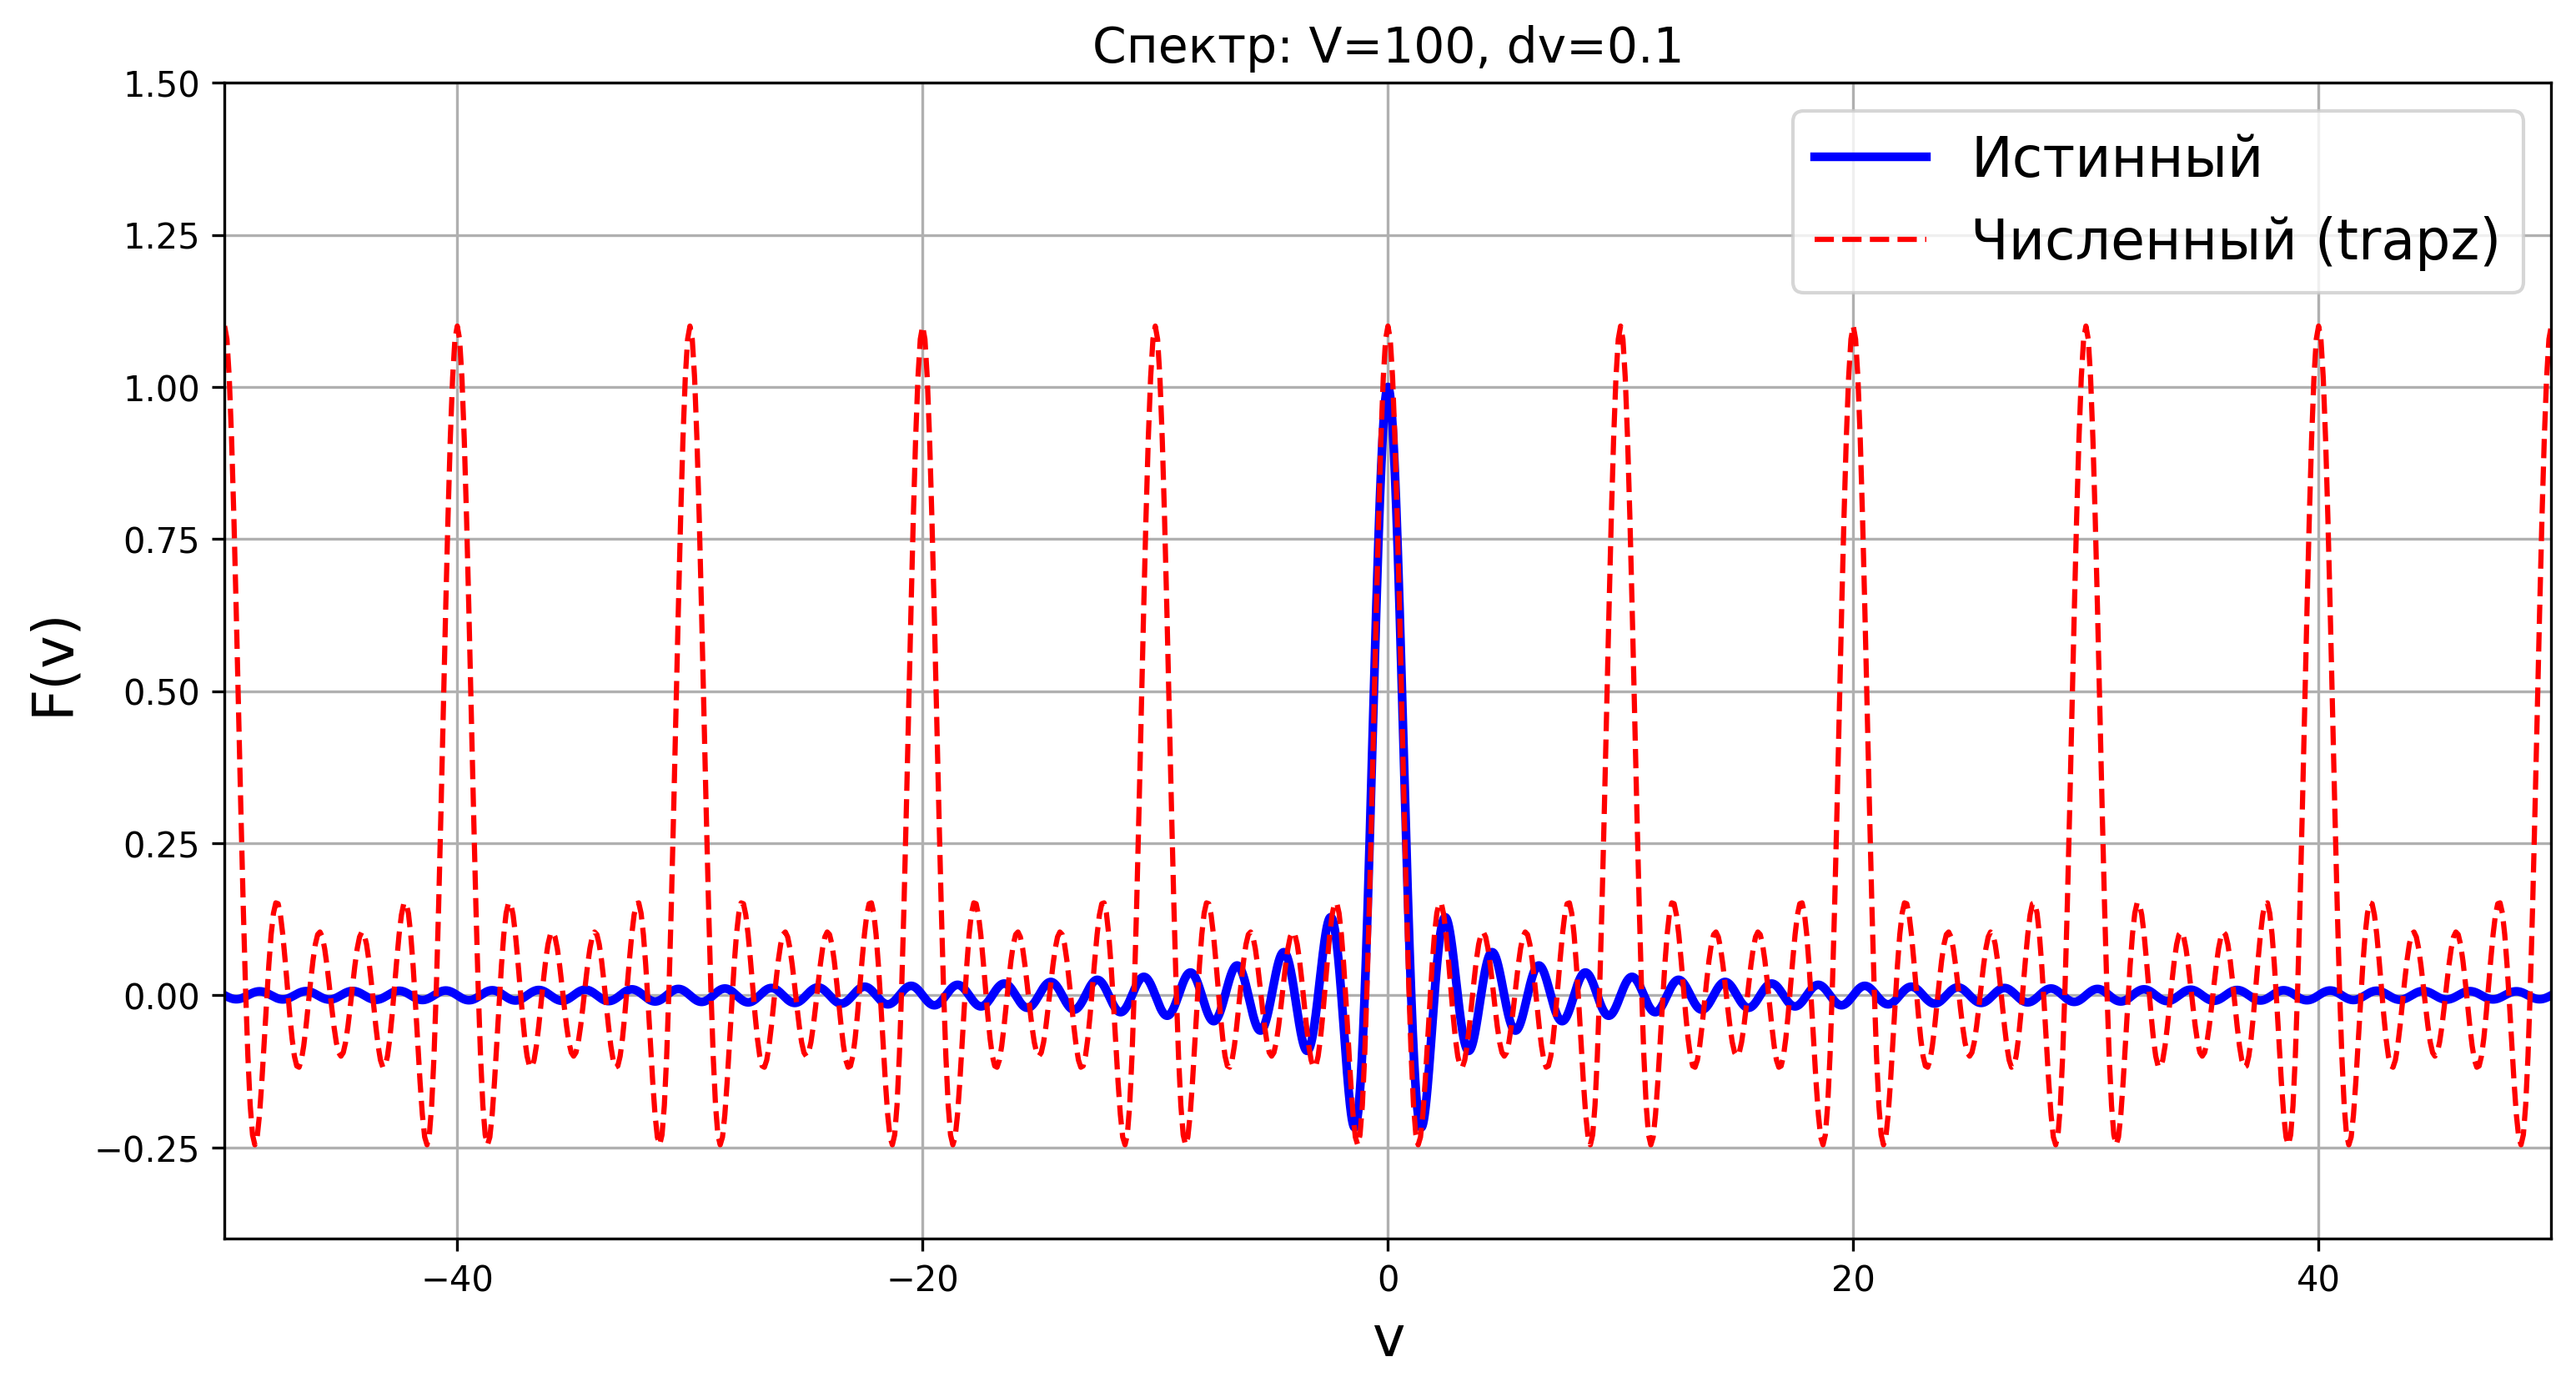
\includegraphics[width=0.95\textwidth]{images/T4_V100_dt0.100_dv0.100_spectrum.png}
    \caption{Сравнение спектров: $V=100$, $dv=0.1$.}
\end{figure}

\newpage
\subsection*{Комбинация 5: $T=4$, $V=100$, $dt=0.01$, $dv=0.5$}

\begin{figure}[H]
    \centering
    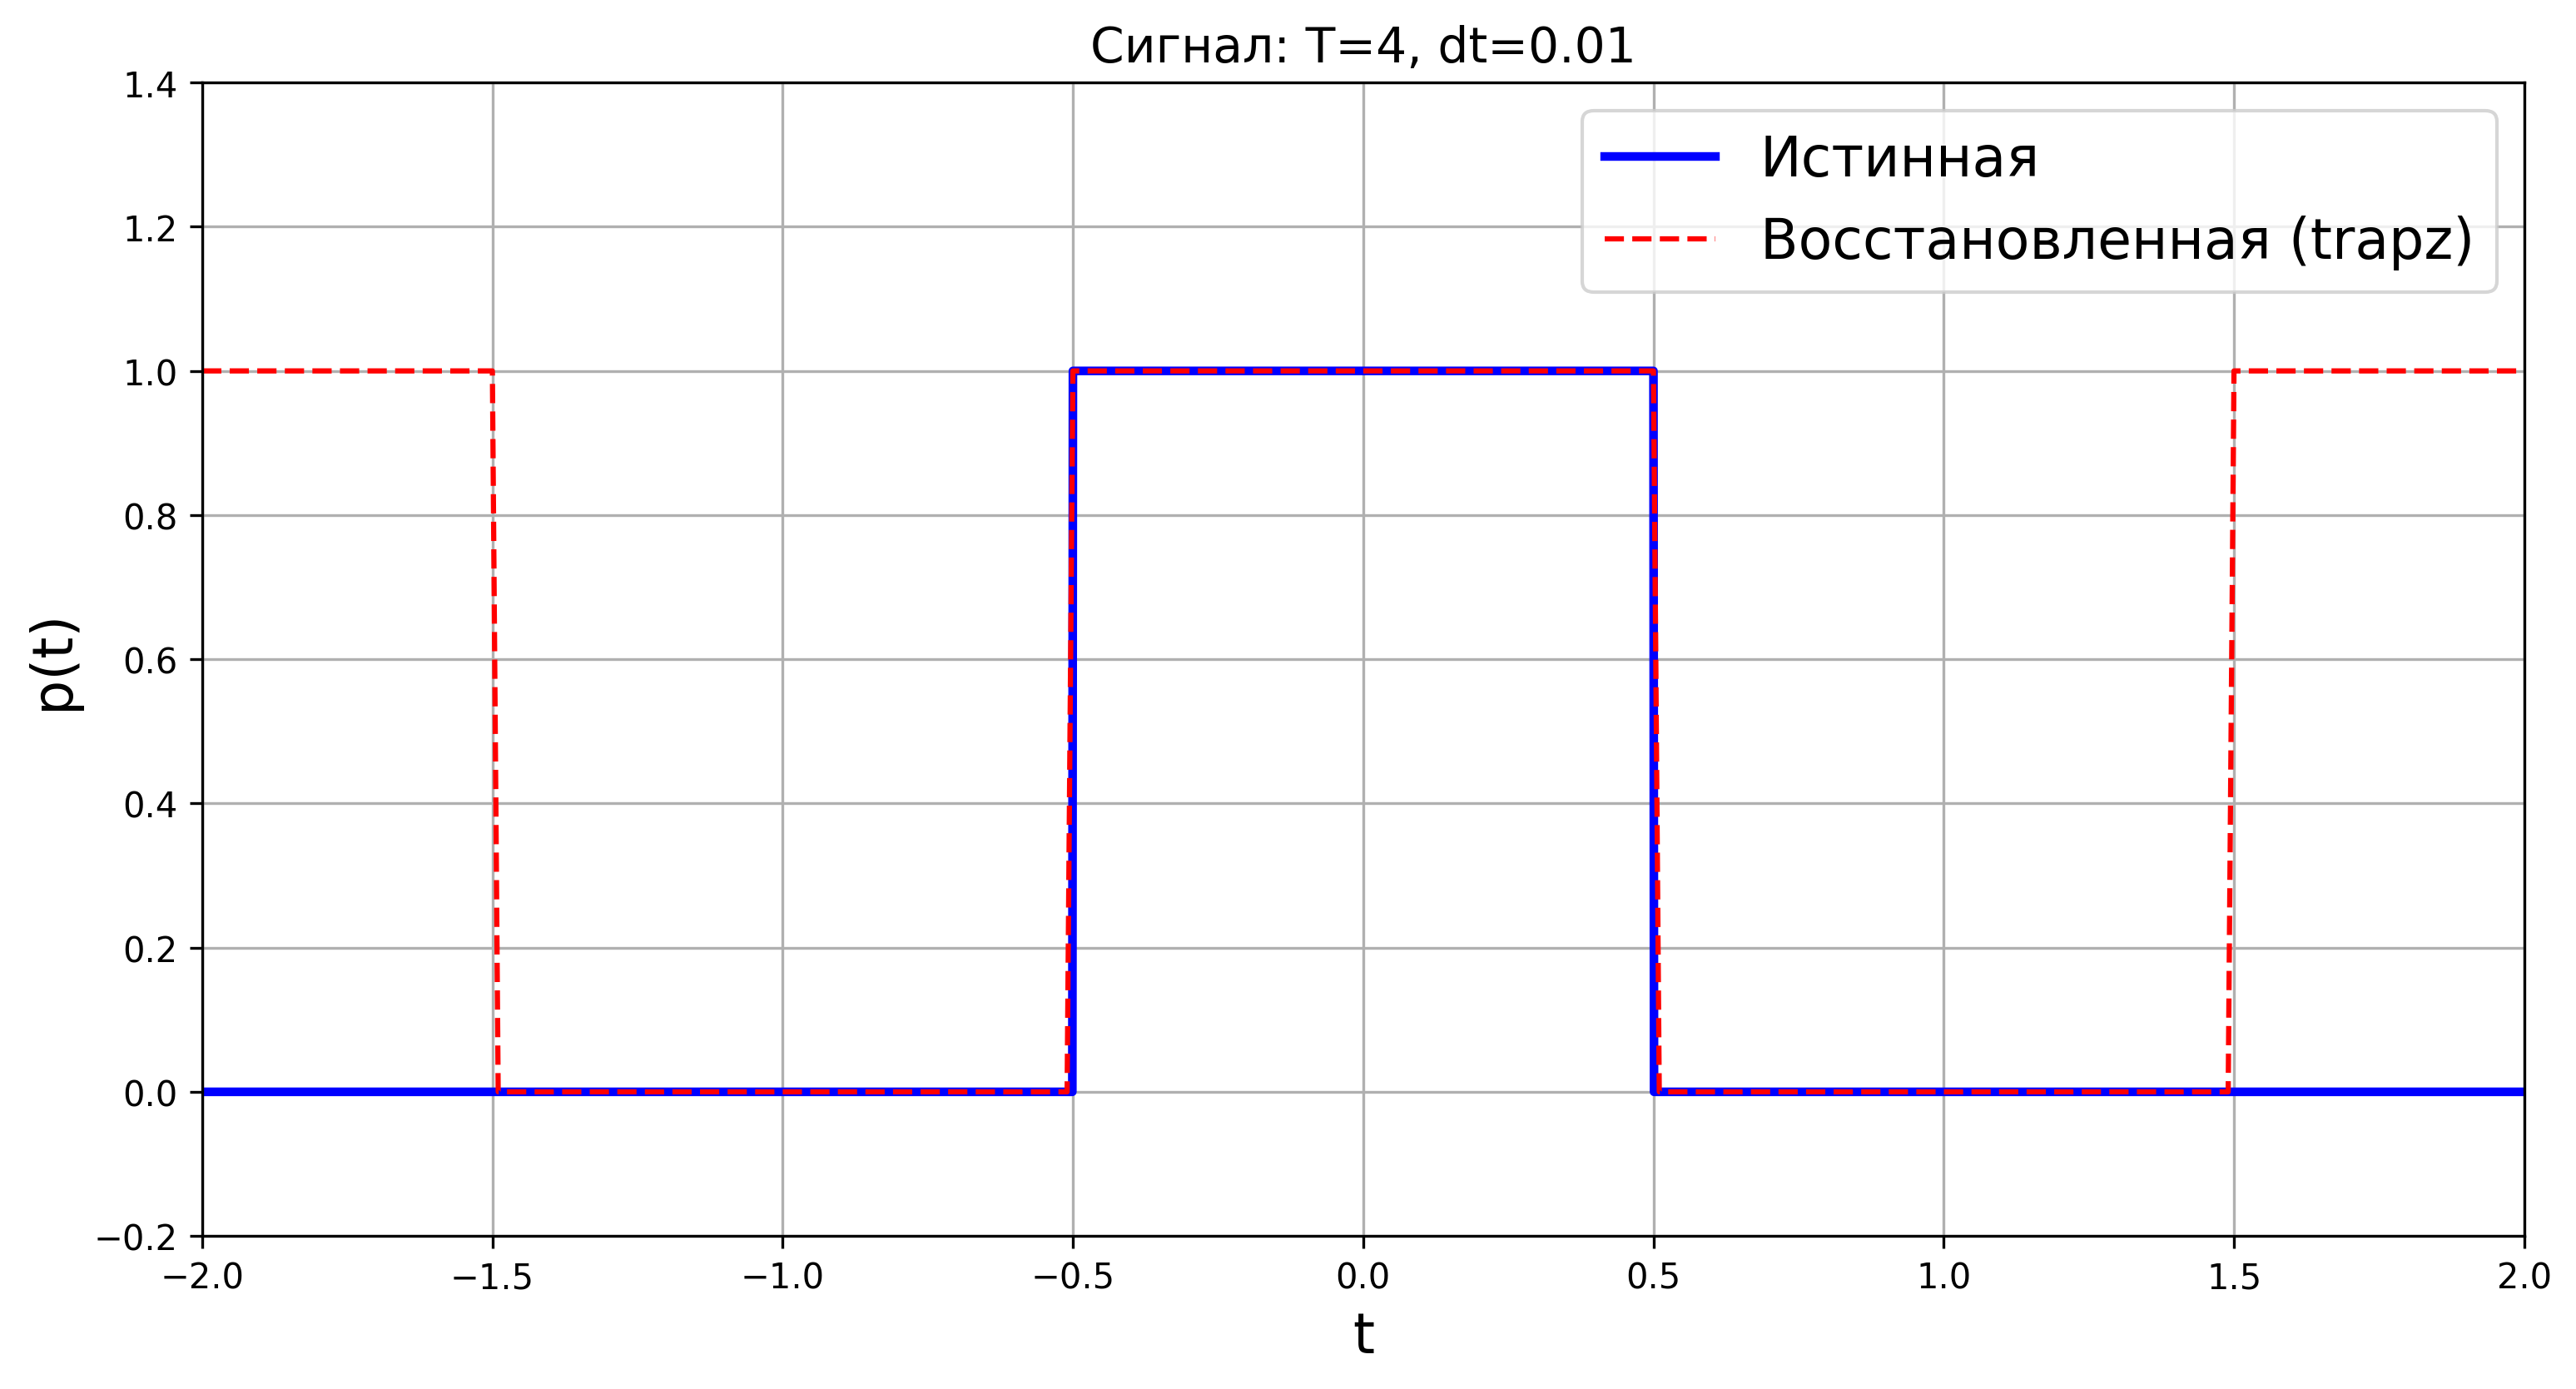
\includegraphics[width=0.95\textwidth]{images/T4_V100_dt0.010_dv0.500_signal.png}
    \caption{Восстановление сигнала: $T=4$, $dt=0.01$.}
\end{figure}

\begin{figure}[H]
    \centering
    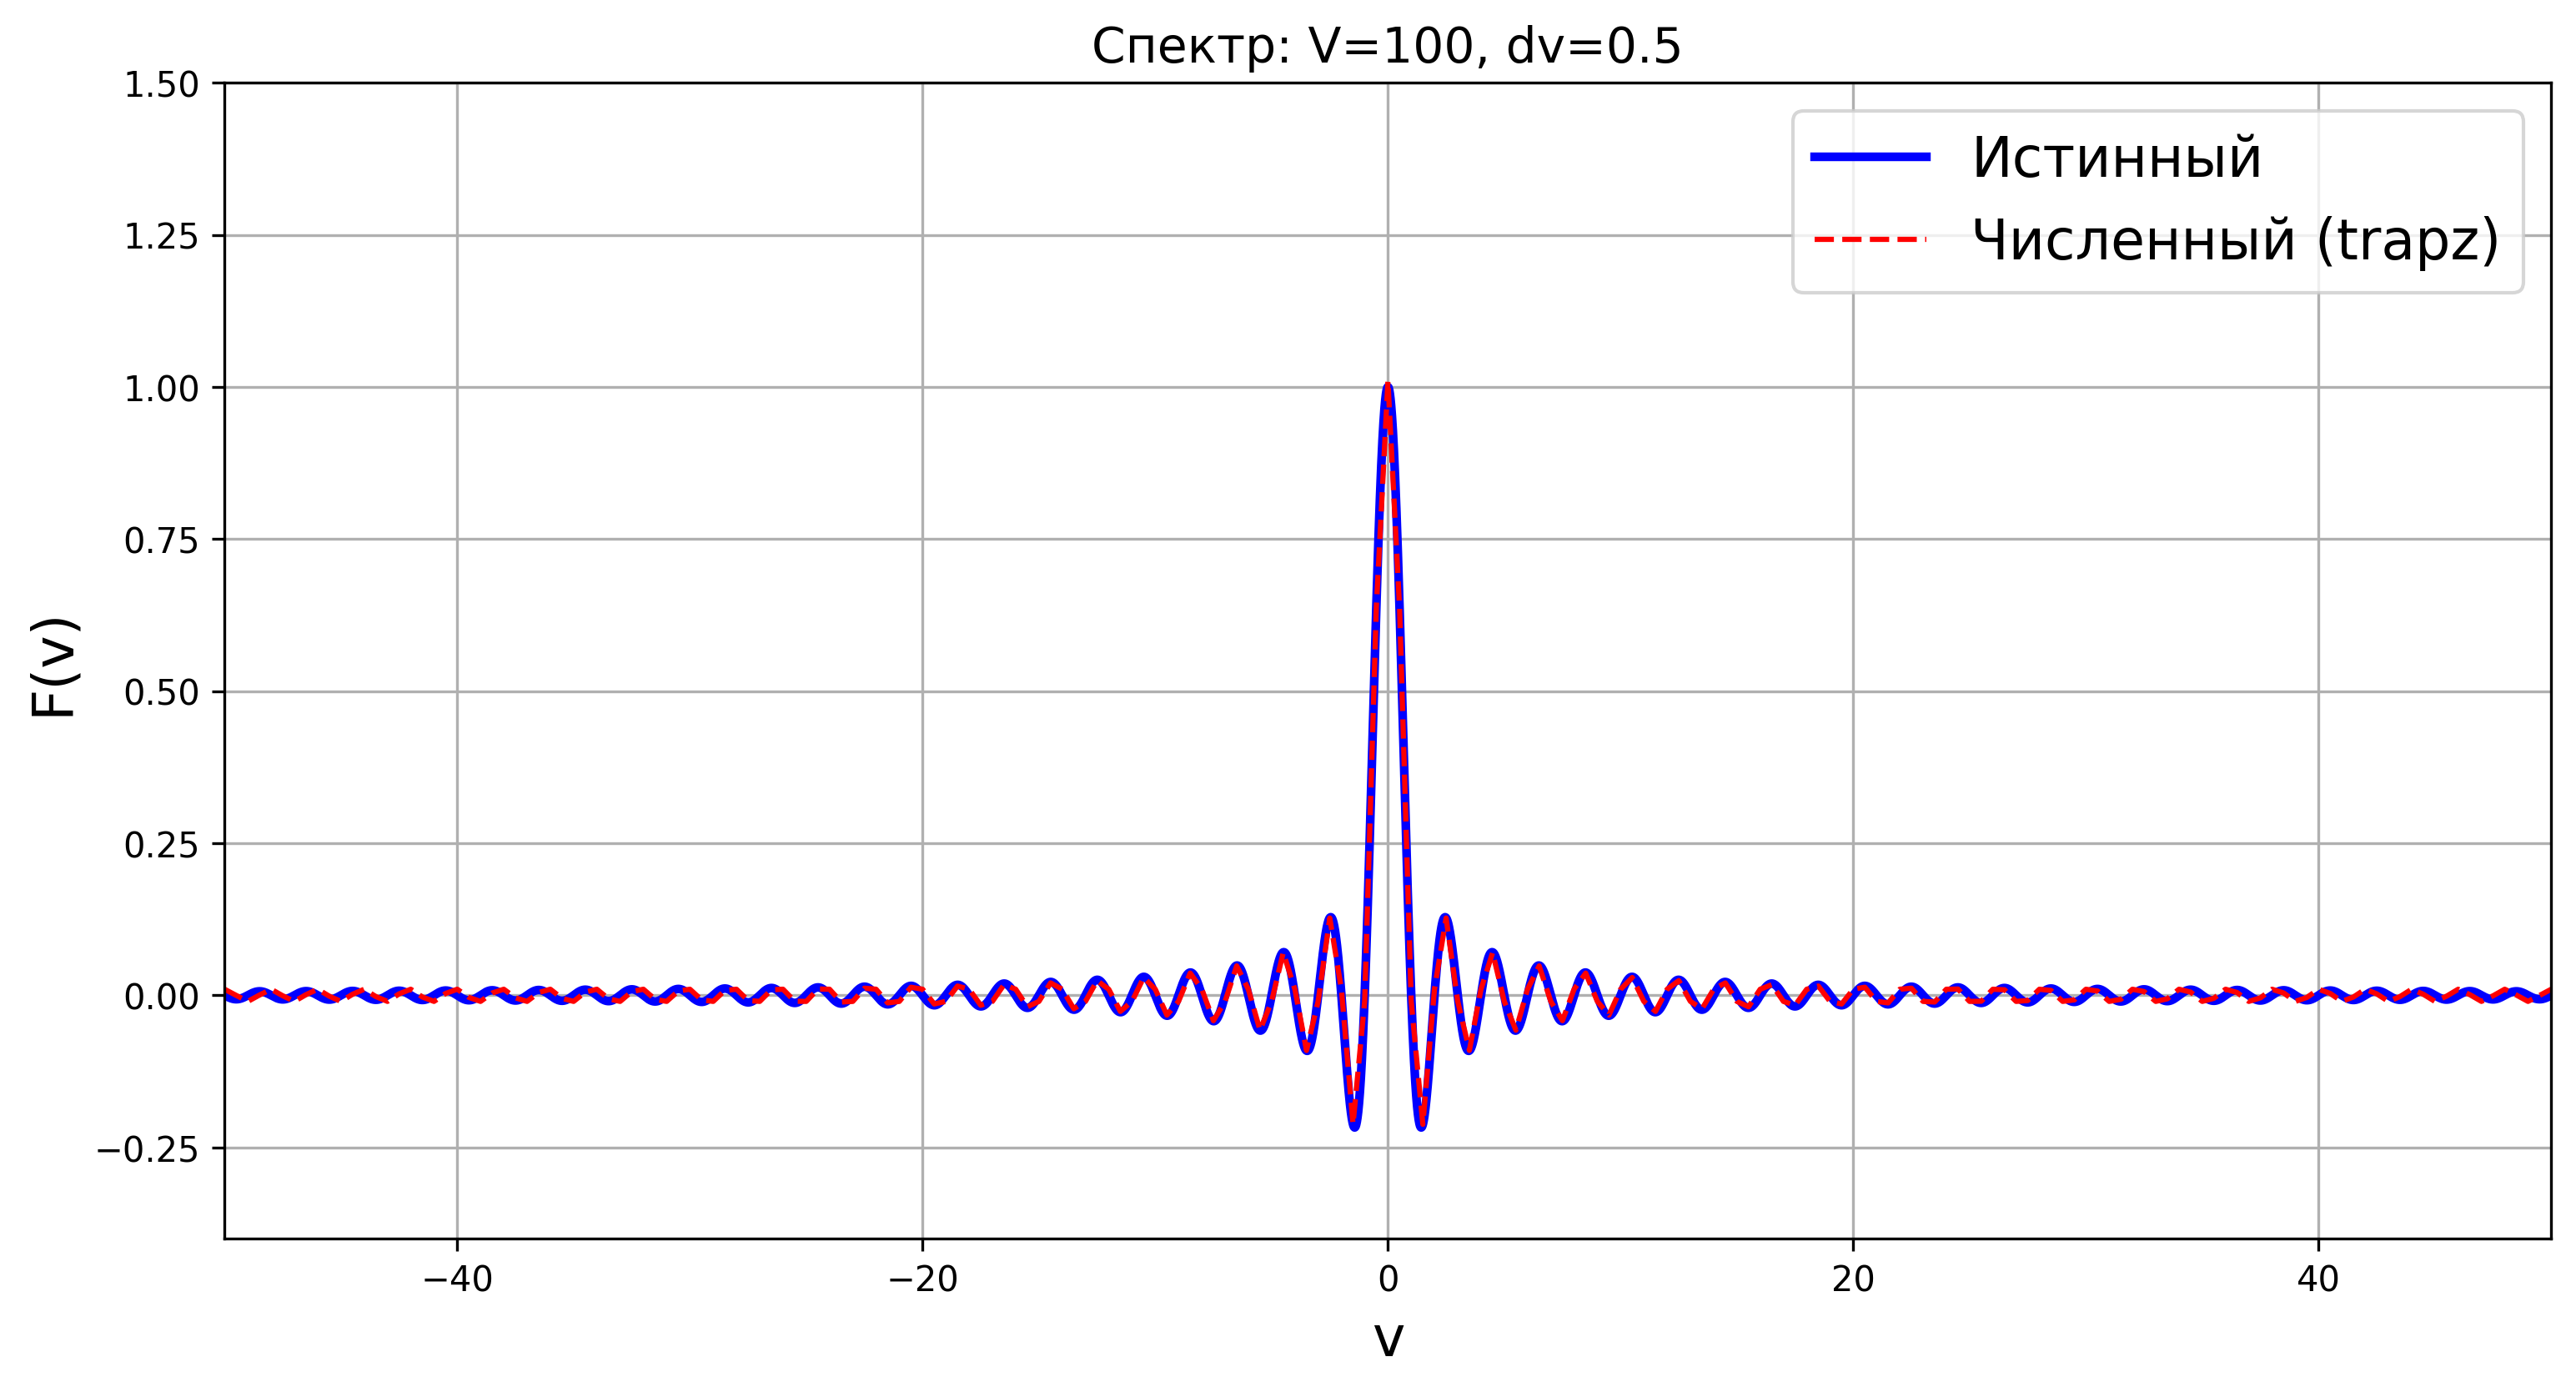
\includegraphics[width=0.95\textwidth]{images/T4_V100_dt0.010_dv0.500_spectrum.png}
    \caption{Сравнение спектров: $V=100$, $dv=0.5$.}
\end{figure}


\newpage



\subsection{Вычисление через FFT}
Для того, чтобы преобразование было унитарным к стандартному преобразованию FFT из numpy добавлены коэффициенты $\frac{1}{\sqrt{N}}$ для прямого преобразования и $\sqrt{N}$ для обратного. Так как в пакете у прямого преобразования коэффициент 1, а у обратного $\frac{1}{N}$
Как видно из перебранных комбинаций, FFT приближает обратное преобразование к функции очень близко, но образ функции достаточно далёк от действительности.

\subsection*{Комбинация 1: $T=4$, $V=100$, $dt=0.01$, $dv=0.1$}

\begin{figure}[H]
    \centering
    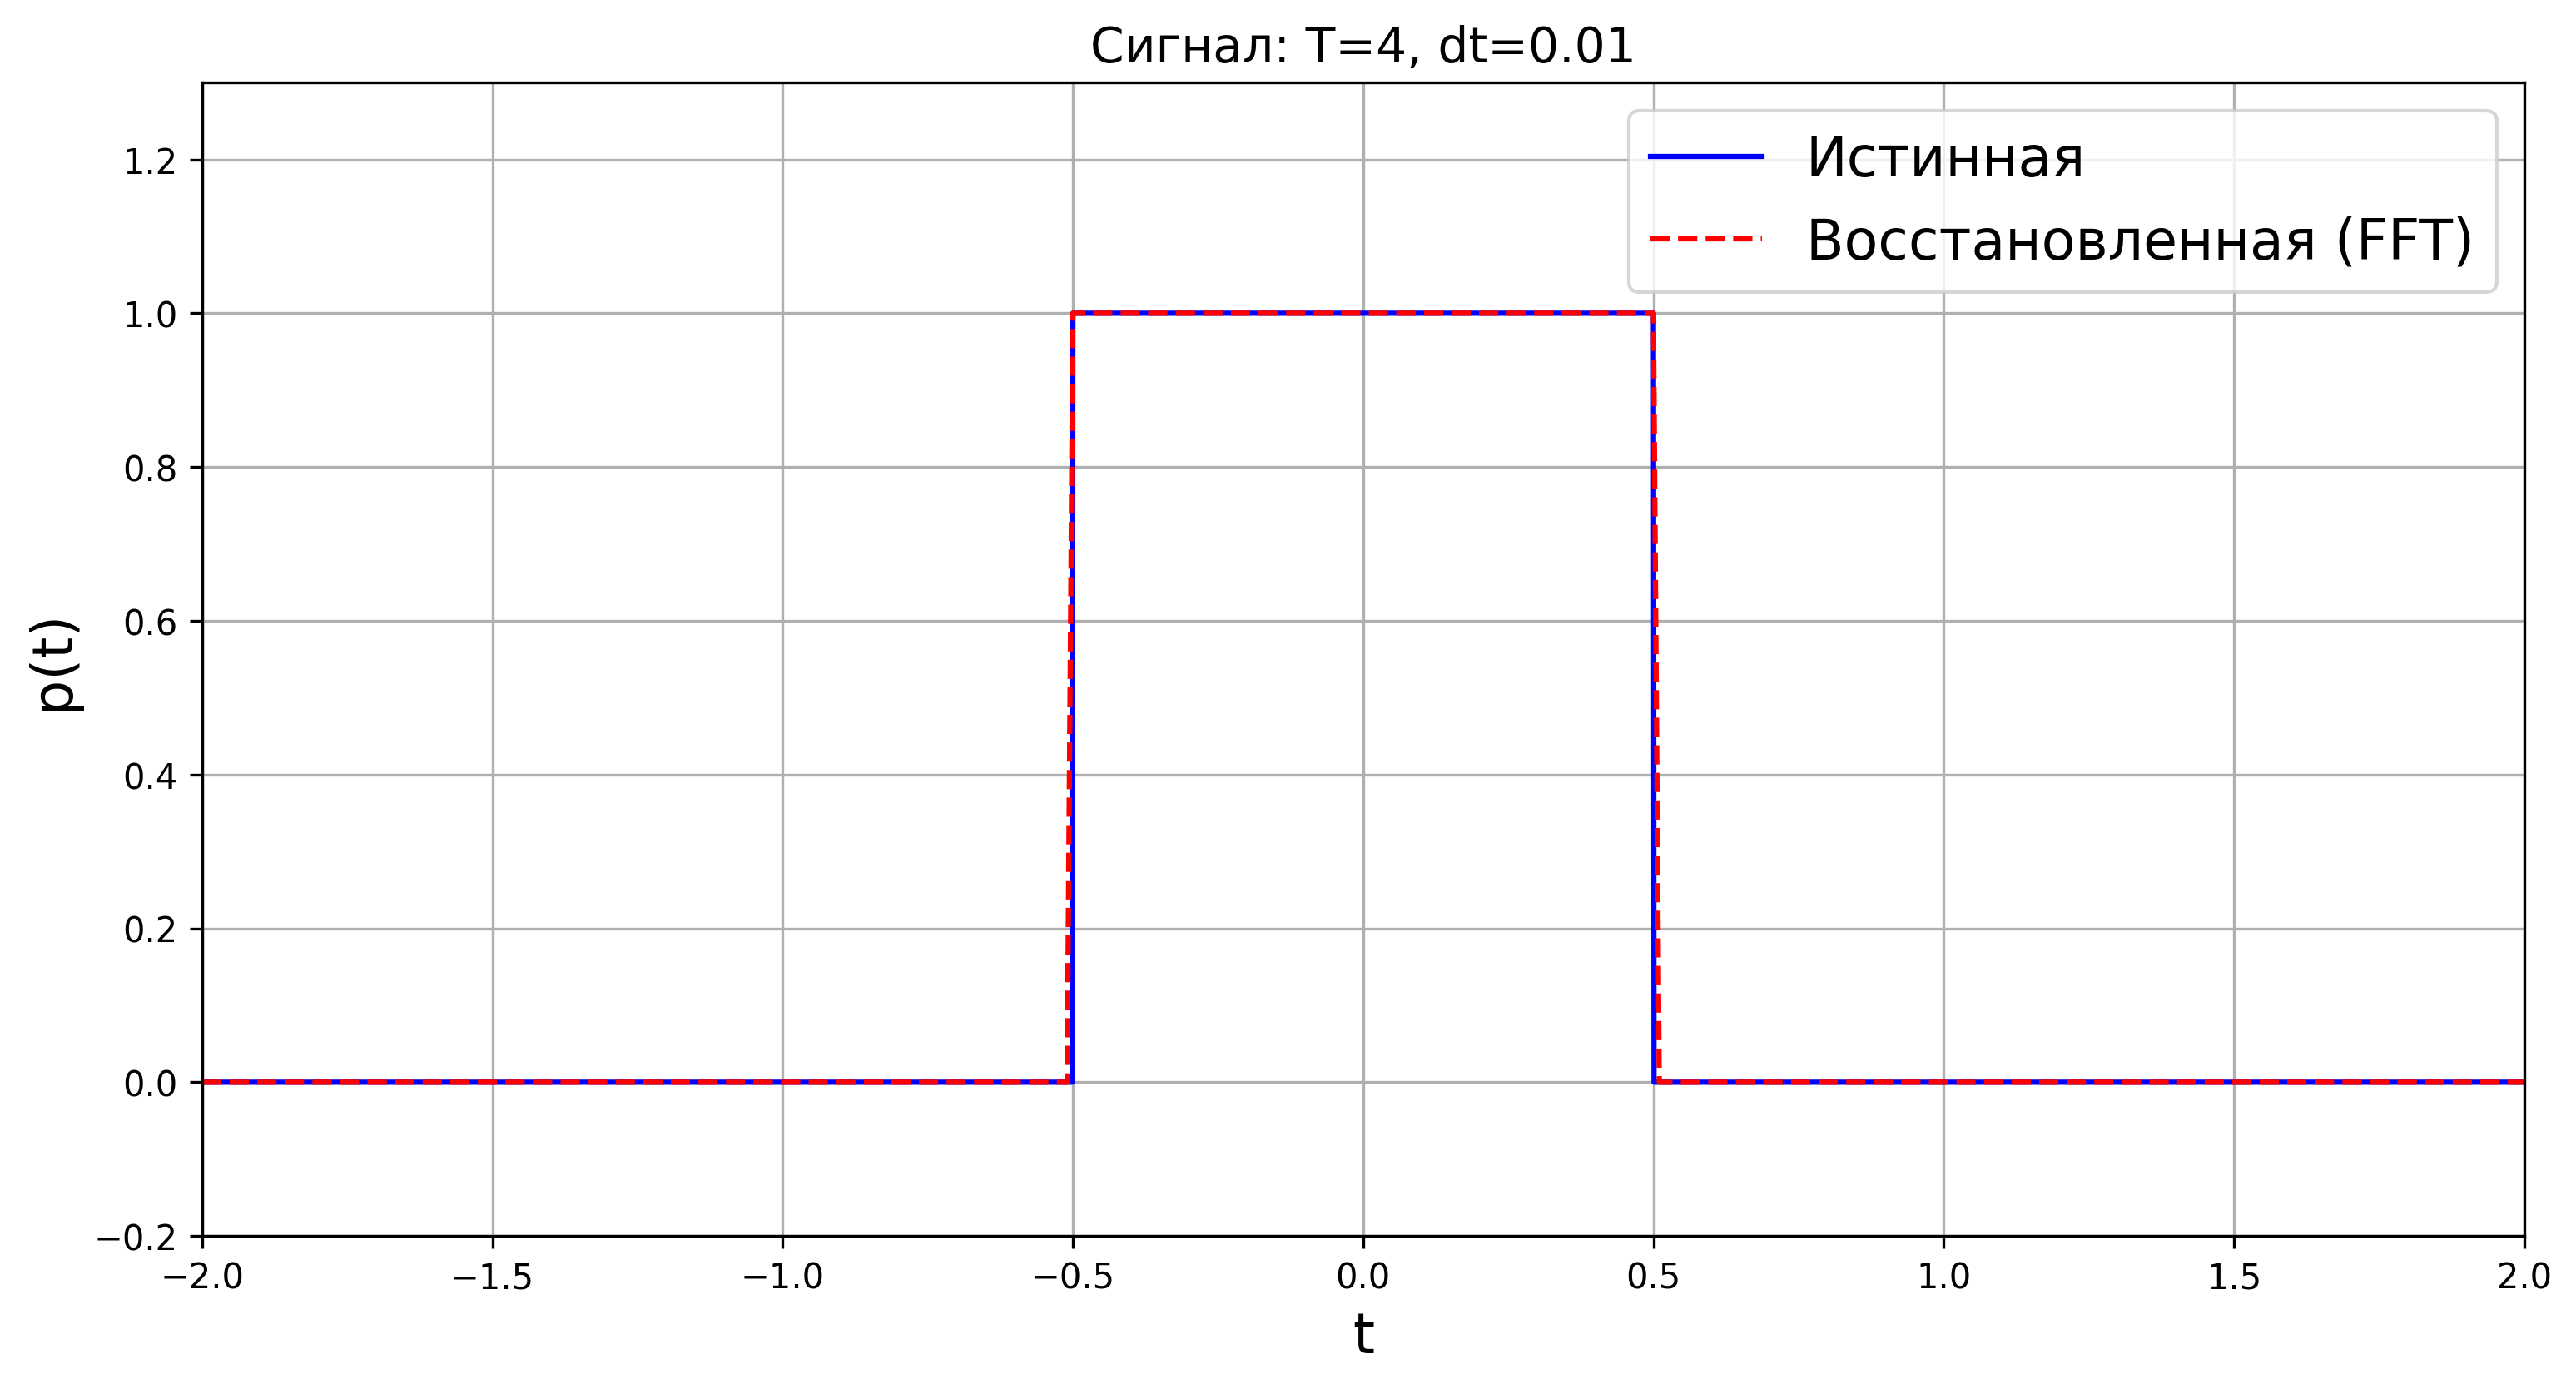
\includegraphics[width=0.95\textwidth]{images/FFT_T4_V100_dt0.010_dv0.100_signal.png}
    \caption{Восстановление сигнала: $T=4$, $dt=0.01$.}
\end{figure}

\begin{figure}[H]
    \centering
    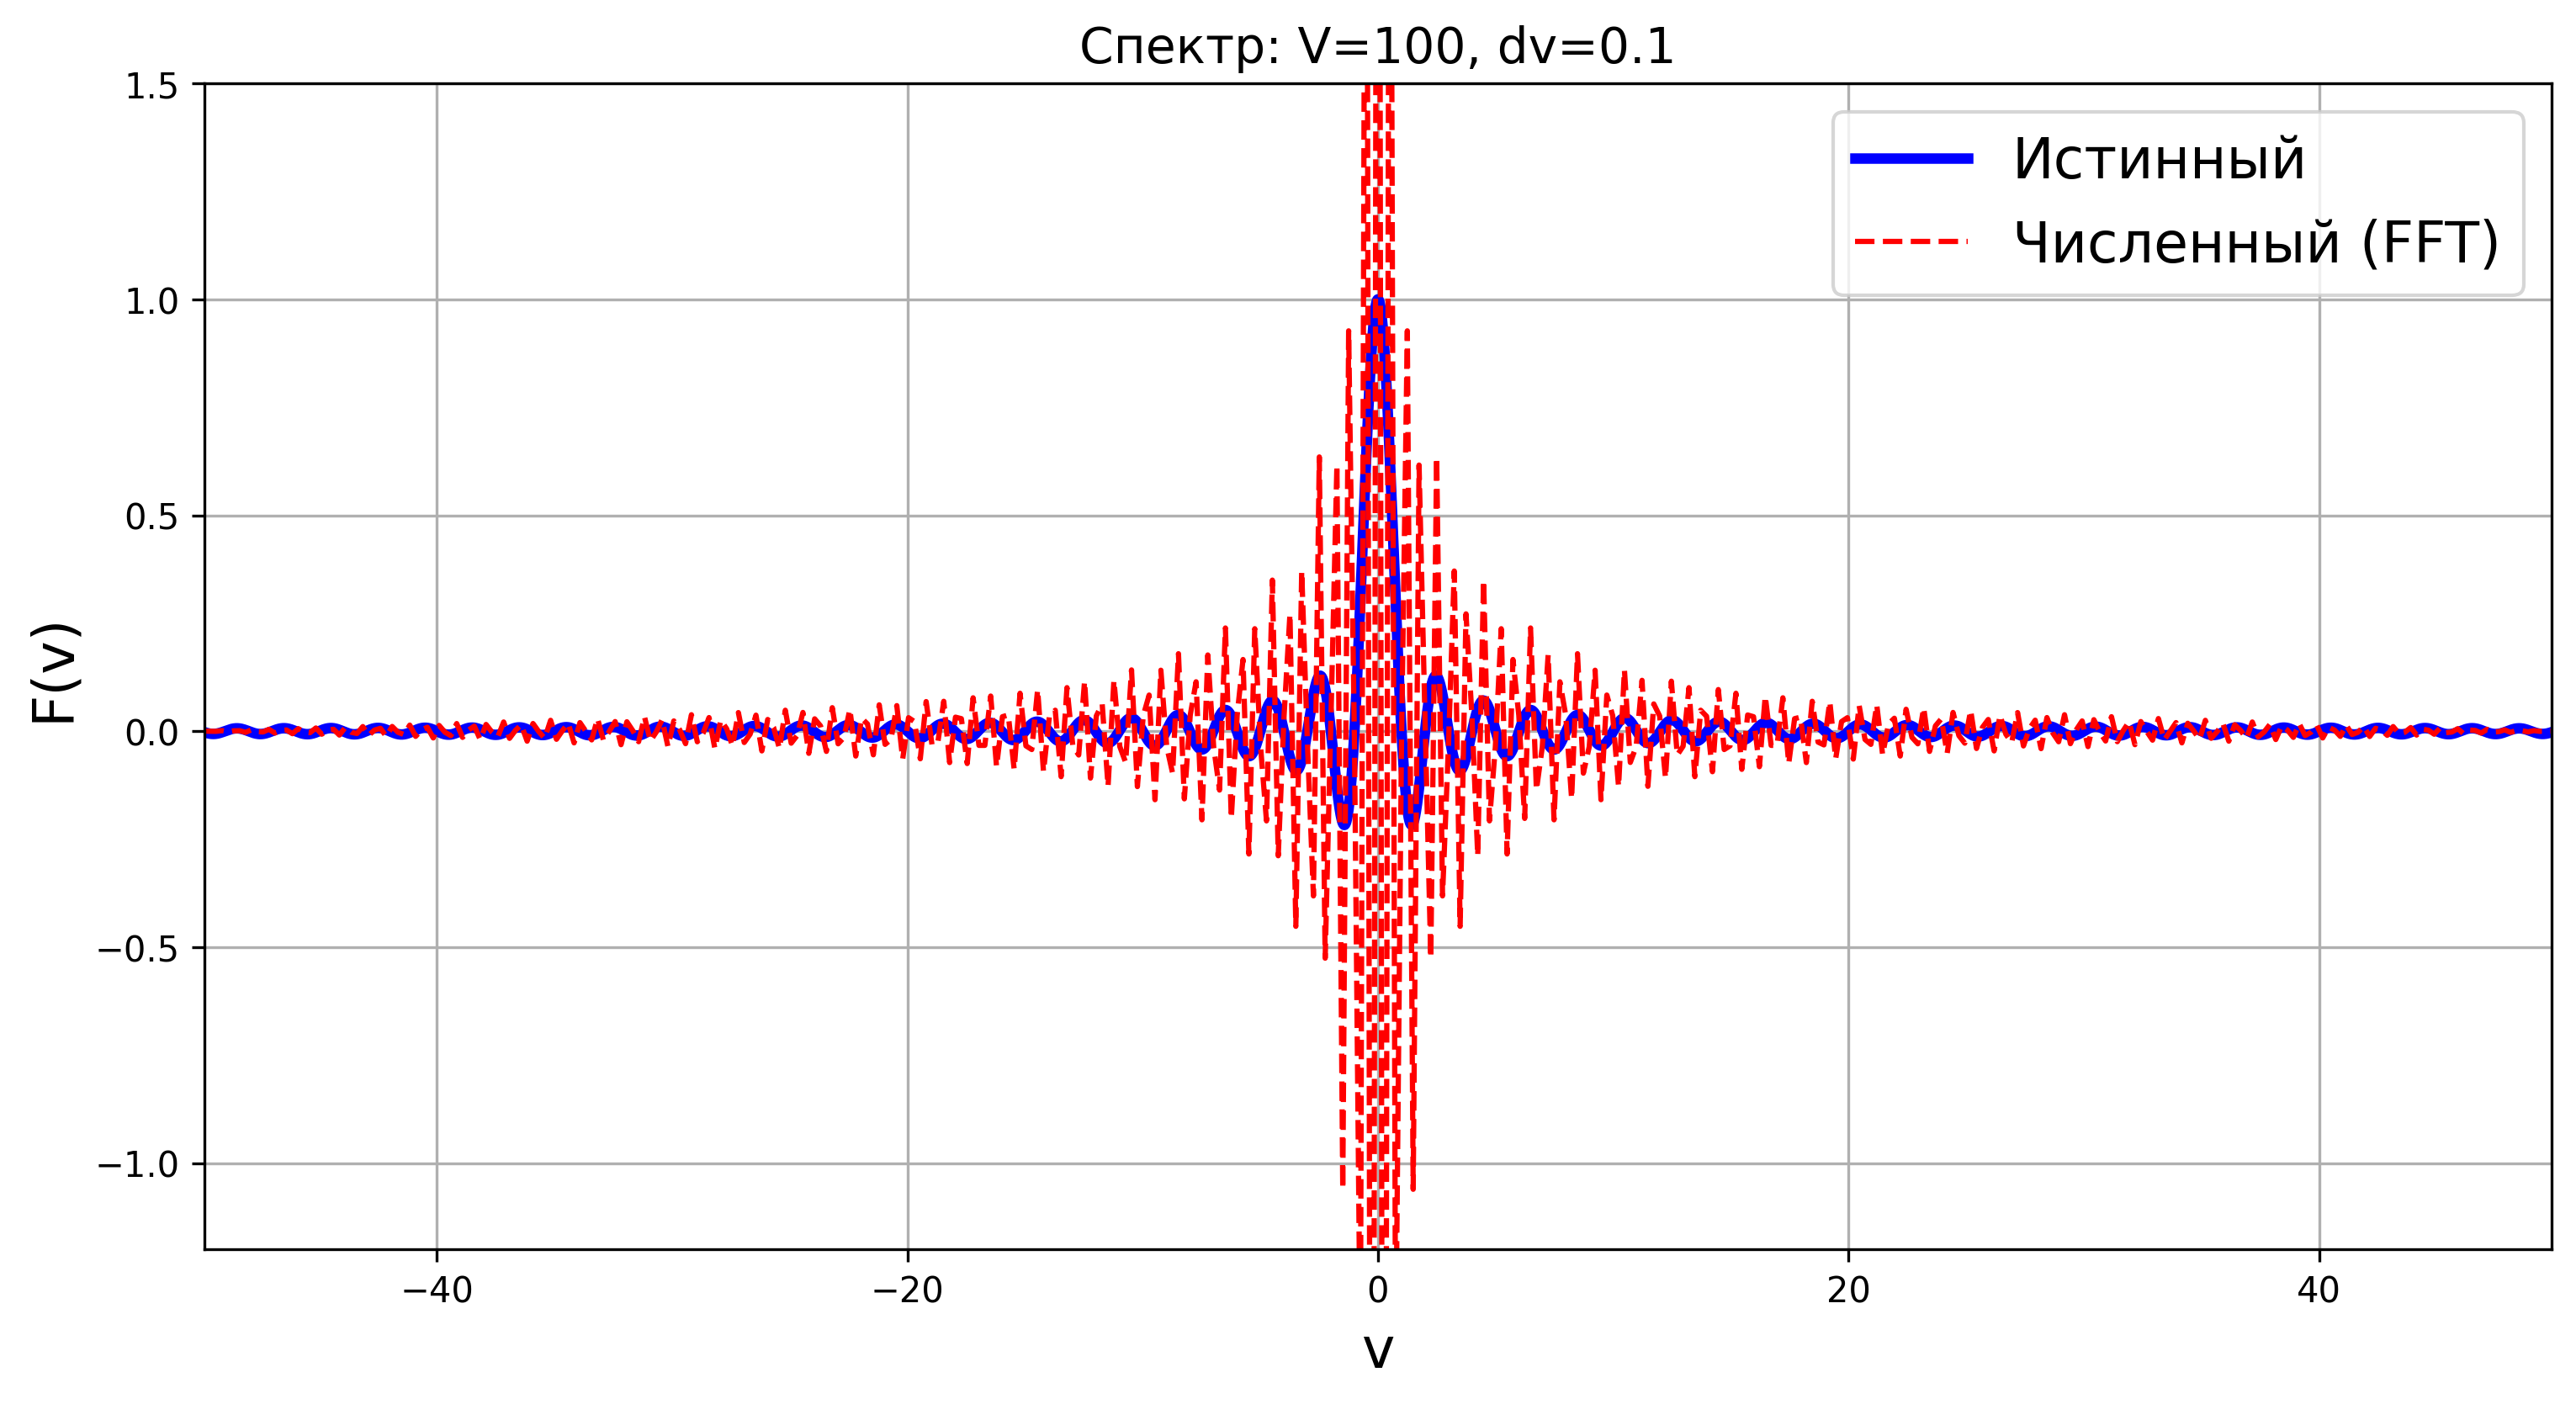
\includegraphics[width=0.95\textwidth]{images/FFT_T4_V100_dt0.010_dv0.100_spectrum.png}
    \caption{Сравнение спектров: $V=100$, $dv=0.1$.}
\end{figure}

\newpage
\subsection*{Комбинация 2: $T=15$, $V=100$, $dt=0.01$, $dv=0.1$}

\begin{figure}[H]
    \centering
    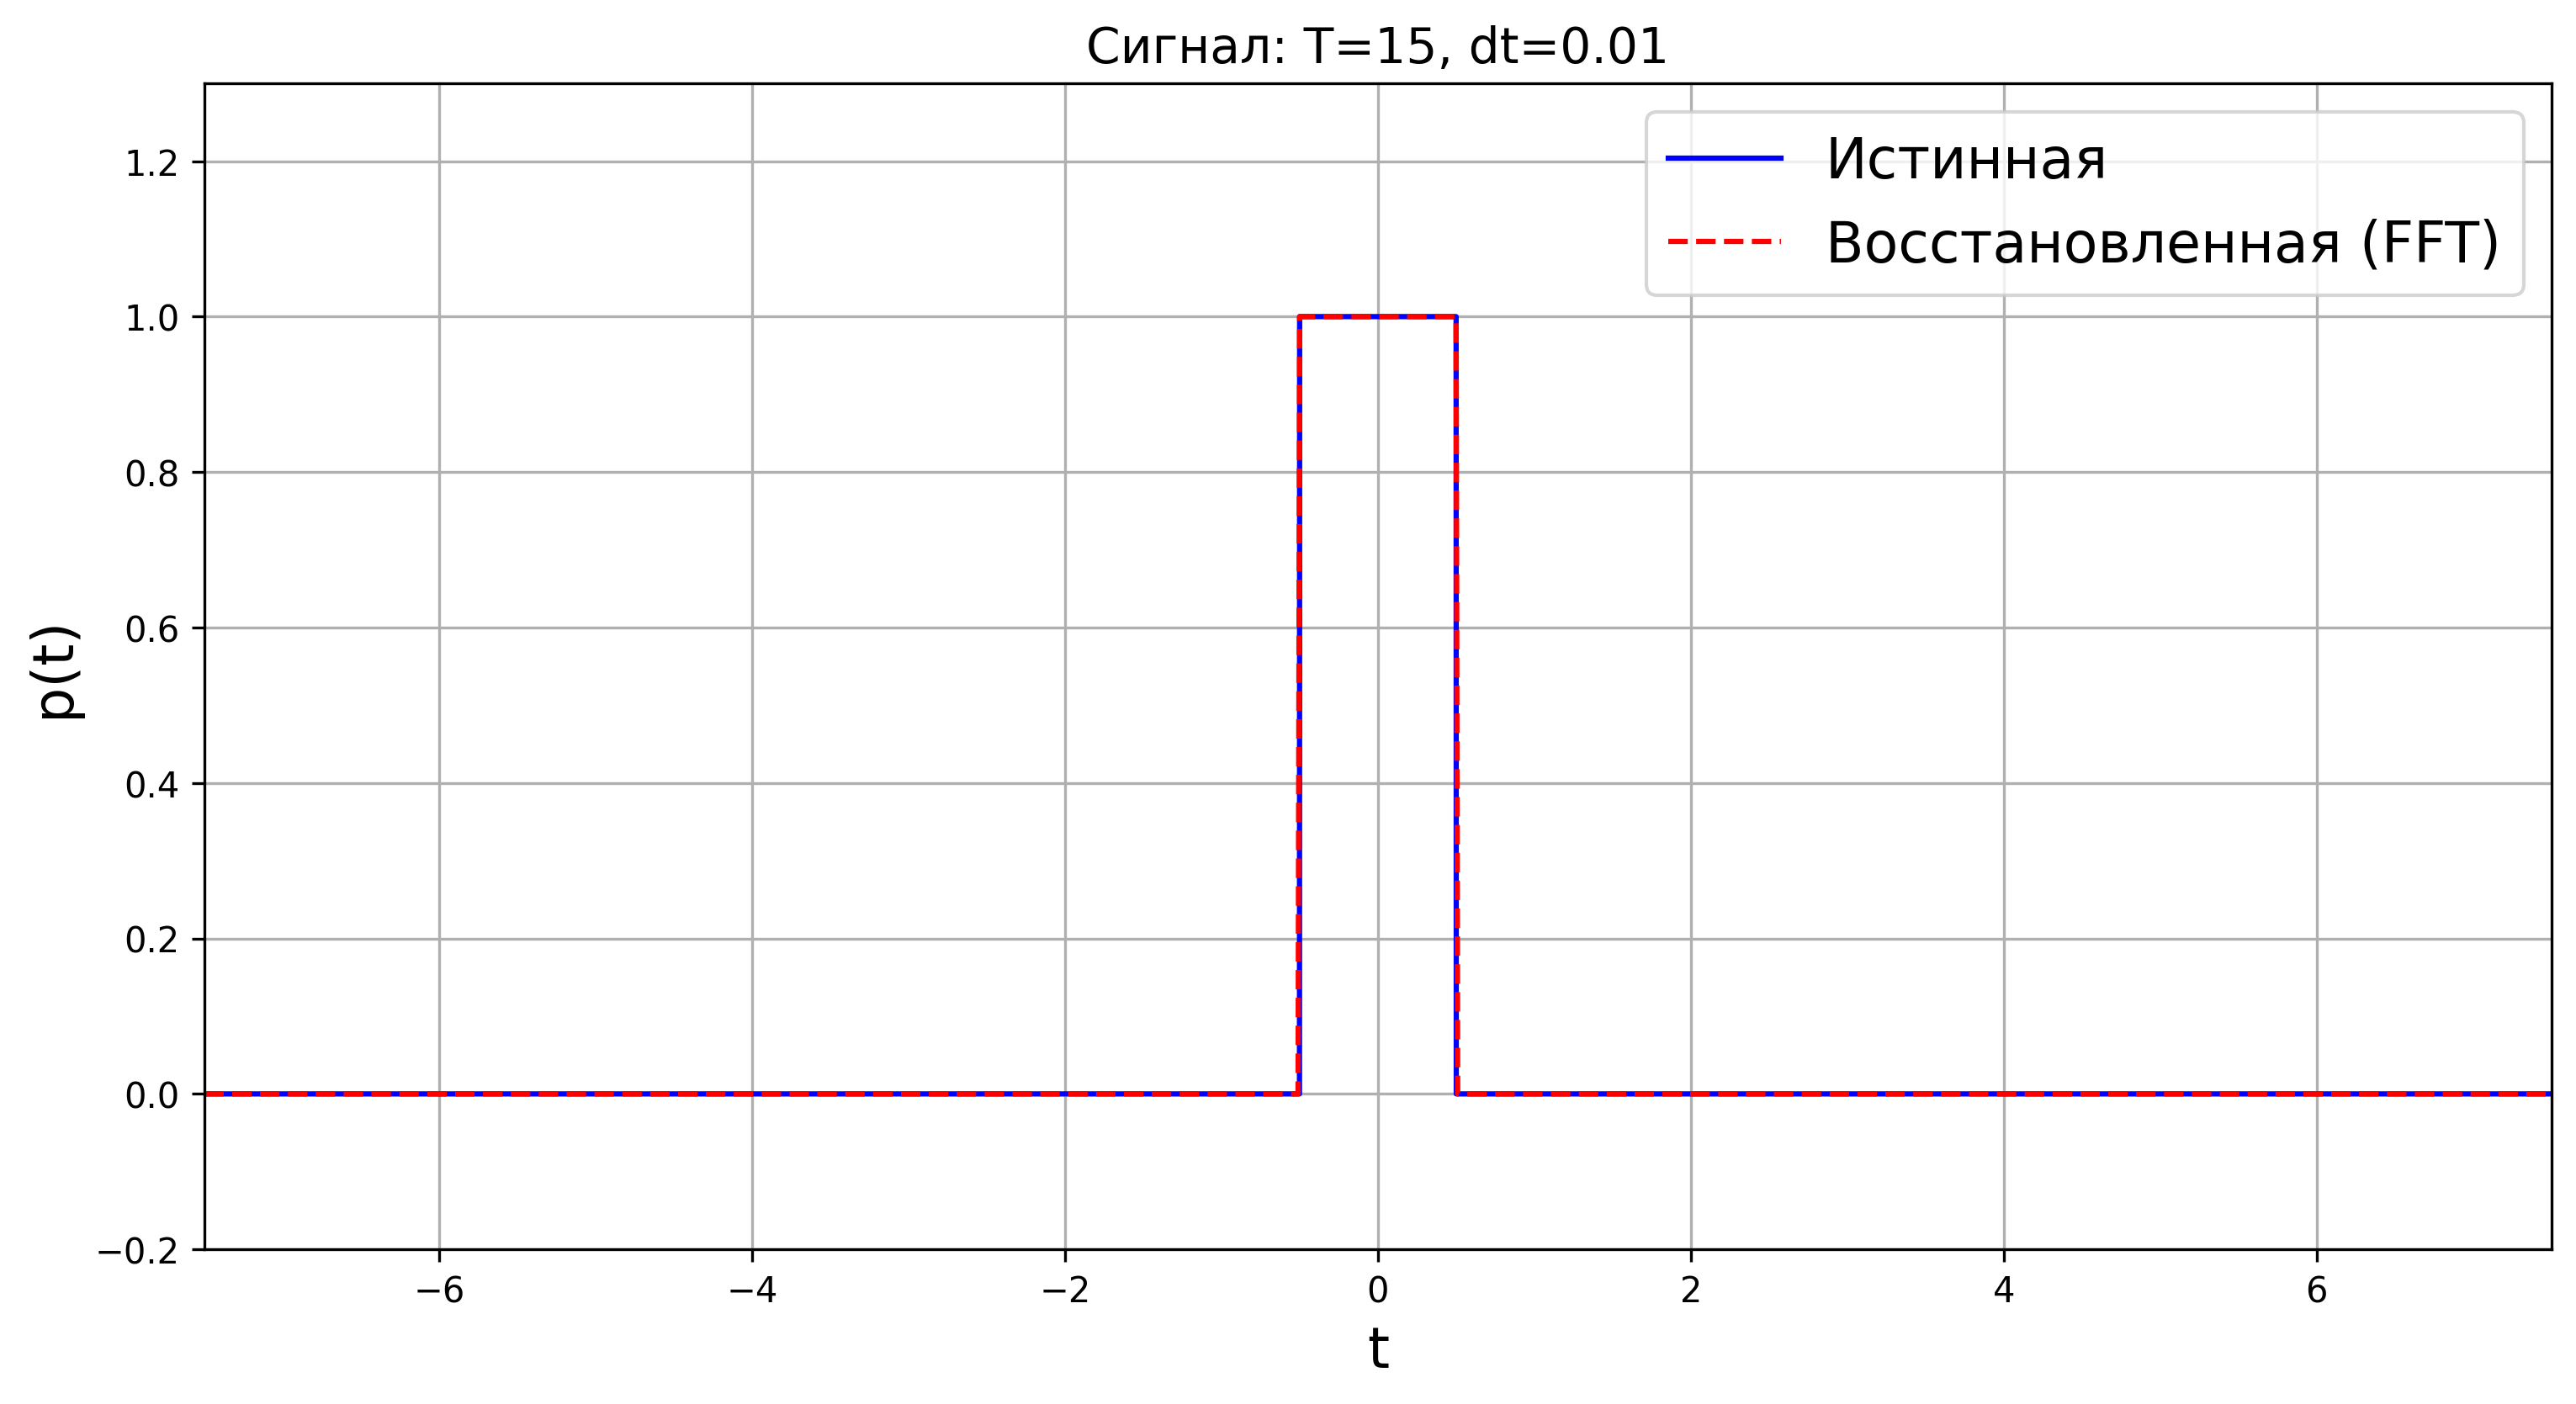
\includegraphics[width=0.95\textwidth]{images/FFT_T15_V100_dt0.010_dv0.100_signal.png}
    \caption{Восстановление сигнала: $T=15$, $dt=0.01$.}
\end{figure}

\begin{figure}[H]
    \centering
    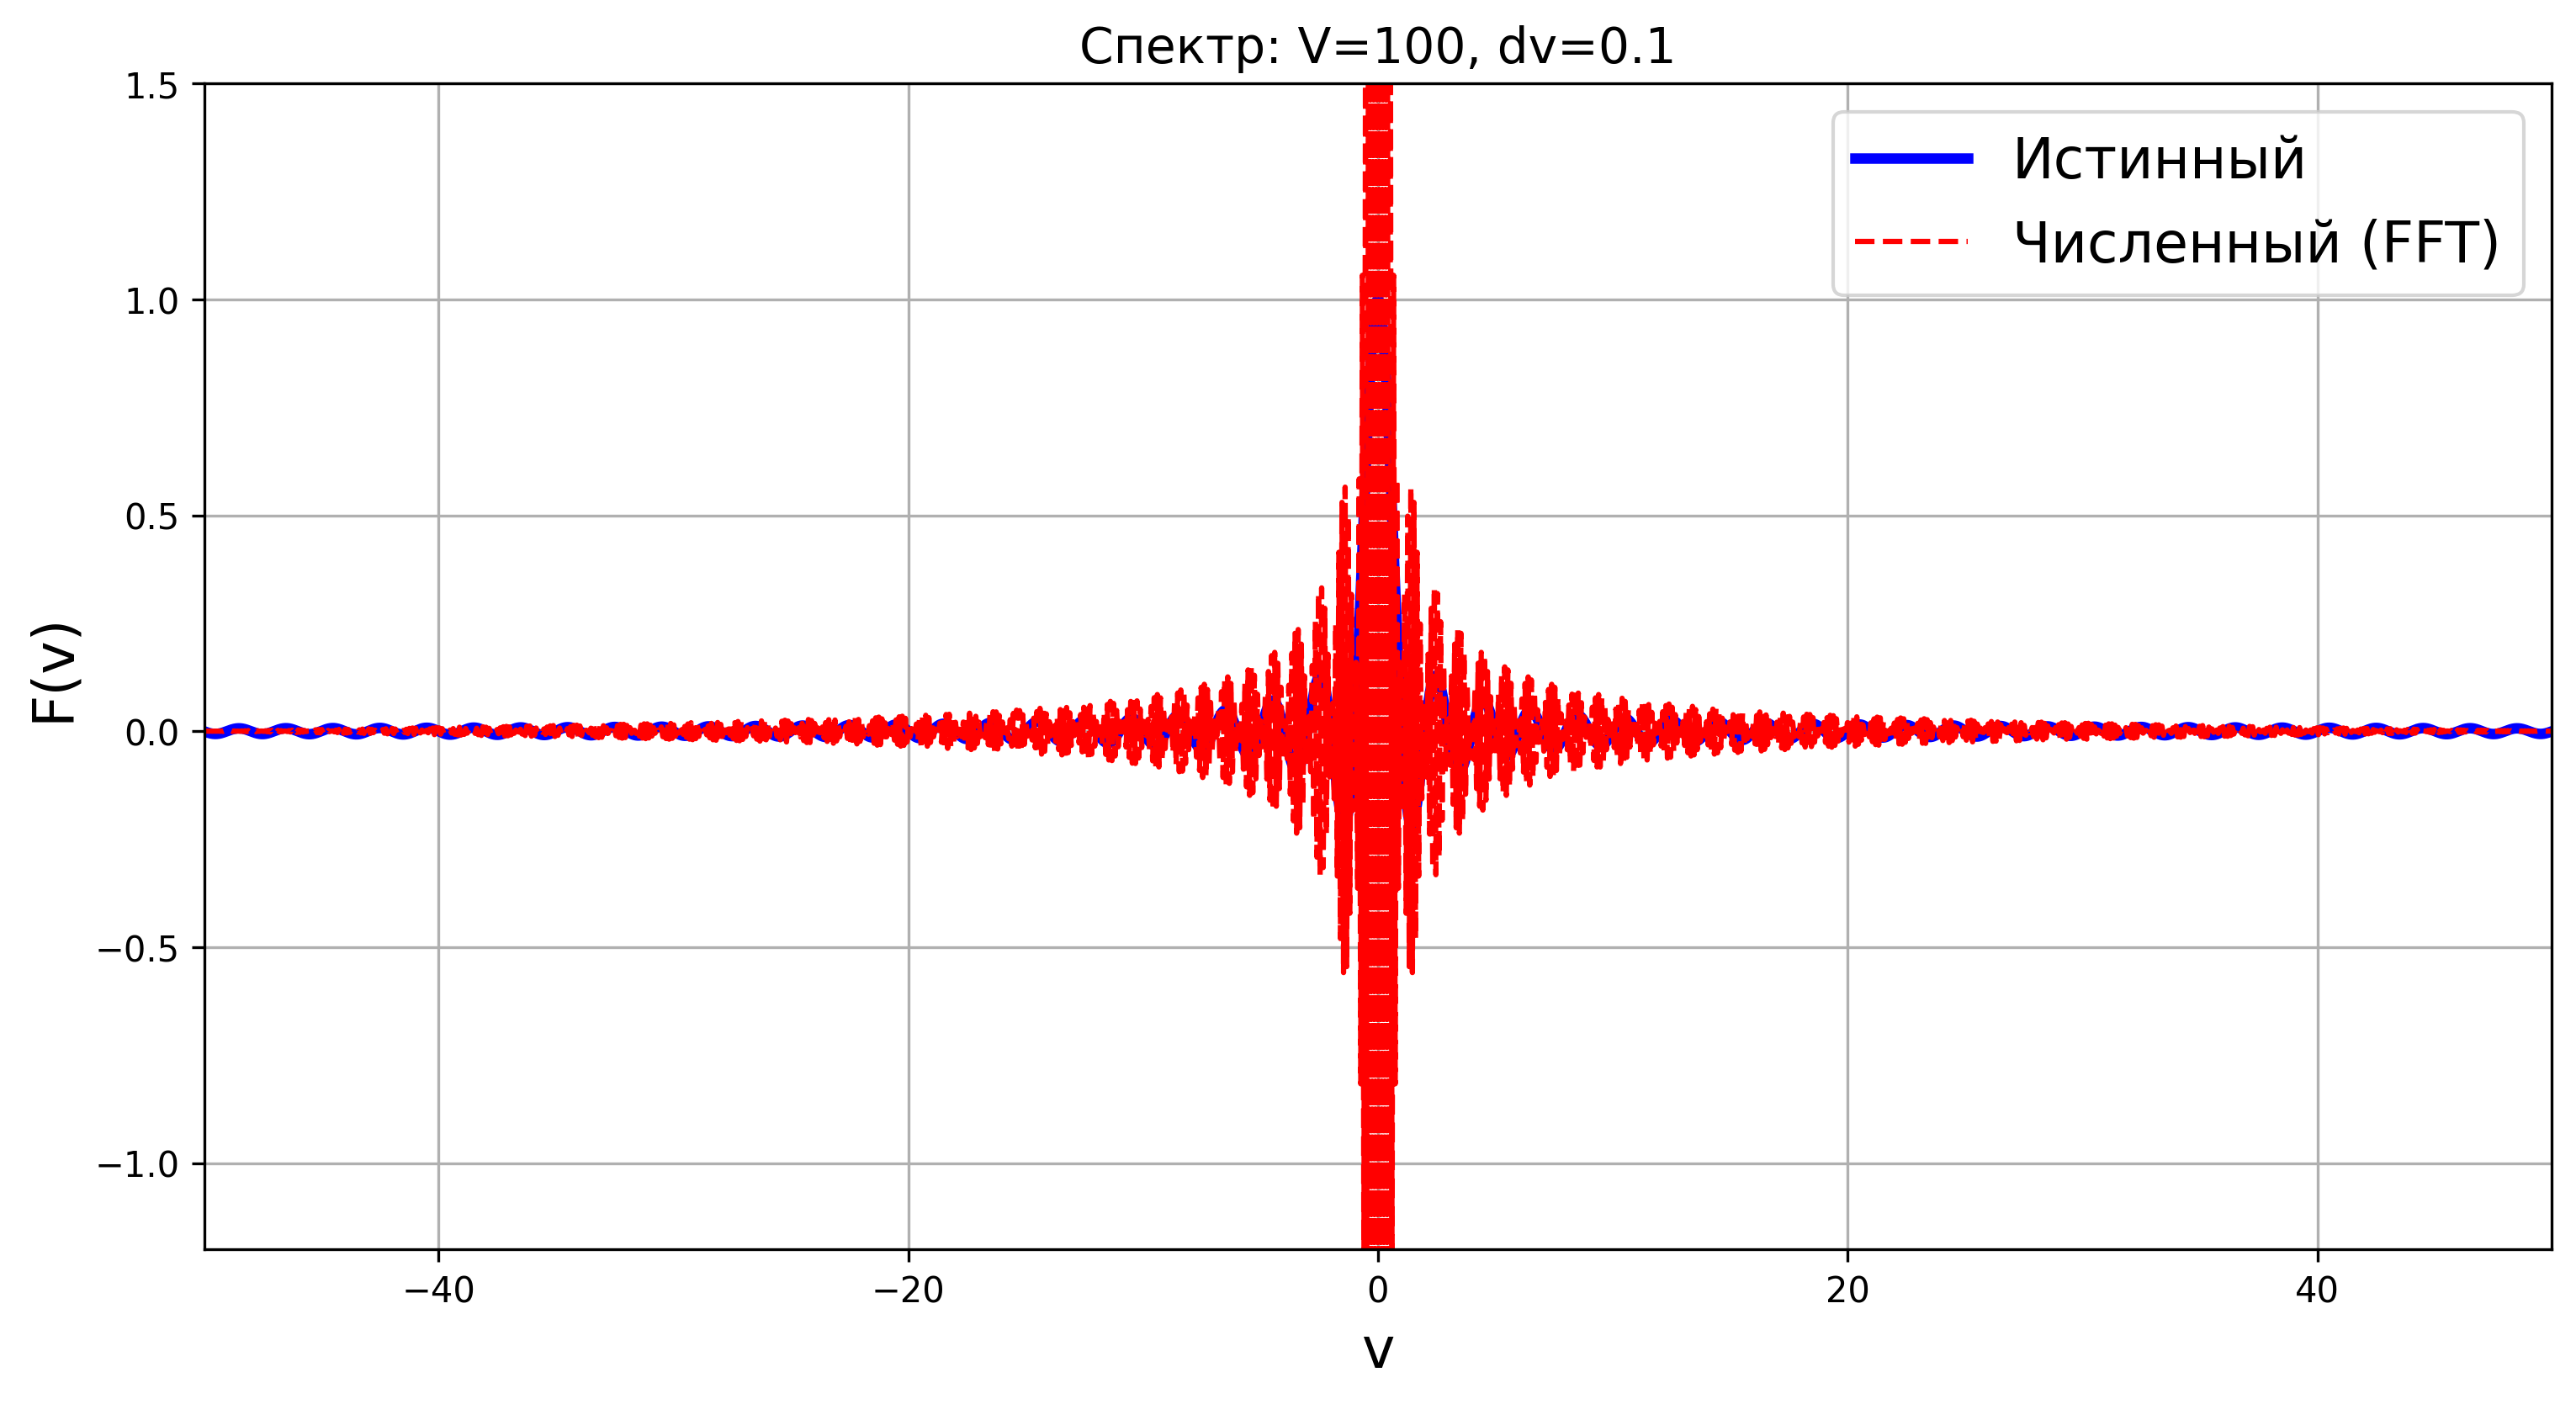
\includegraphics[width=0.95\textwidth]{images/FFT_T15_V100_dt0.010_dv0.100_spectrum.png}
    \caption{Сравнение спектров: $V=100$, $dv=0.1$.}
\end{figure}

\newpage
\subsection*{Комбинация 3: $T=4$, $V=200$, $dt=0.01$, $dv=0.1$}

\begin{figure}[H]
    \centering
    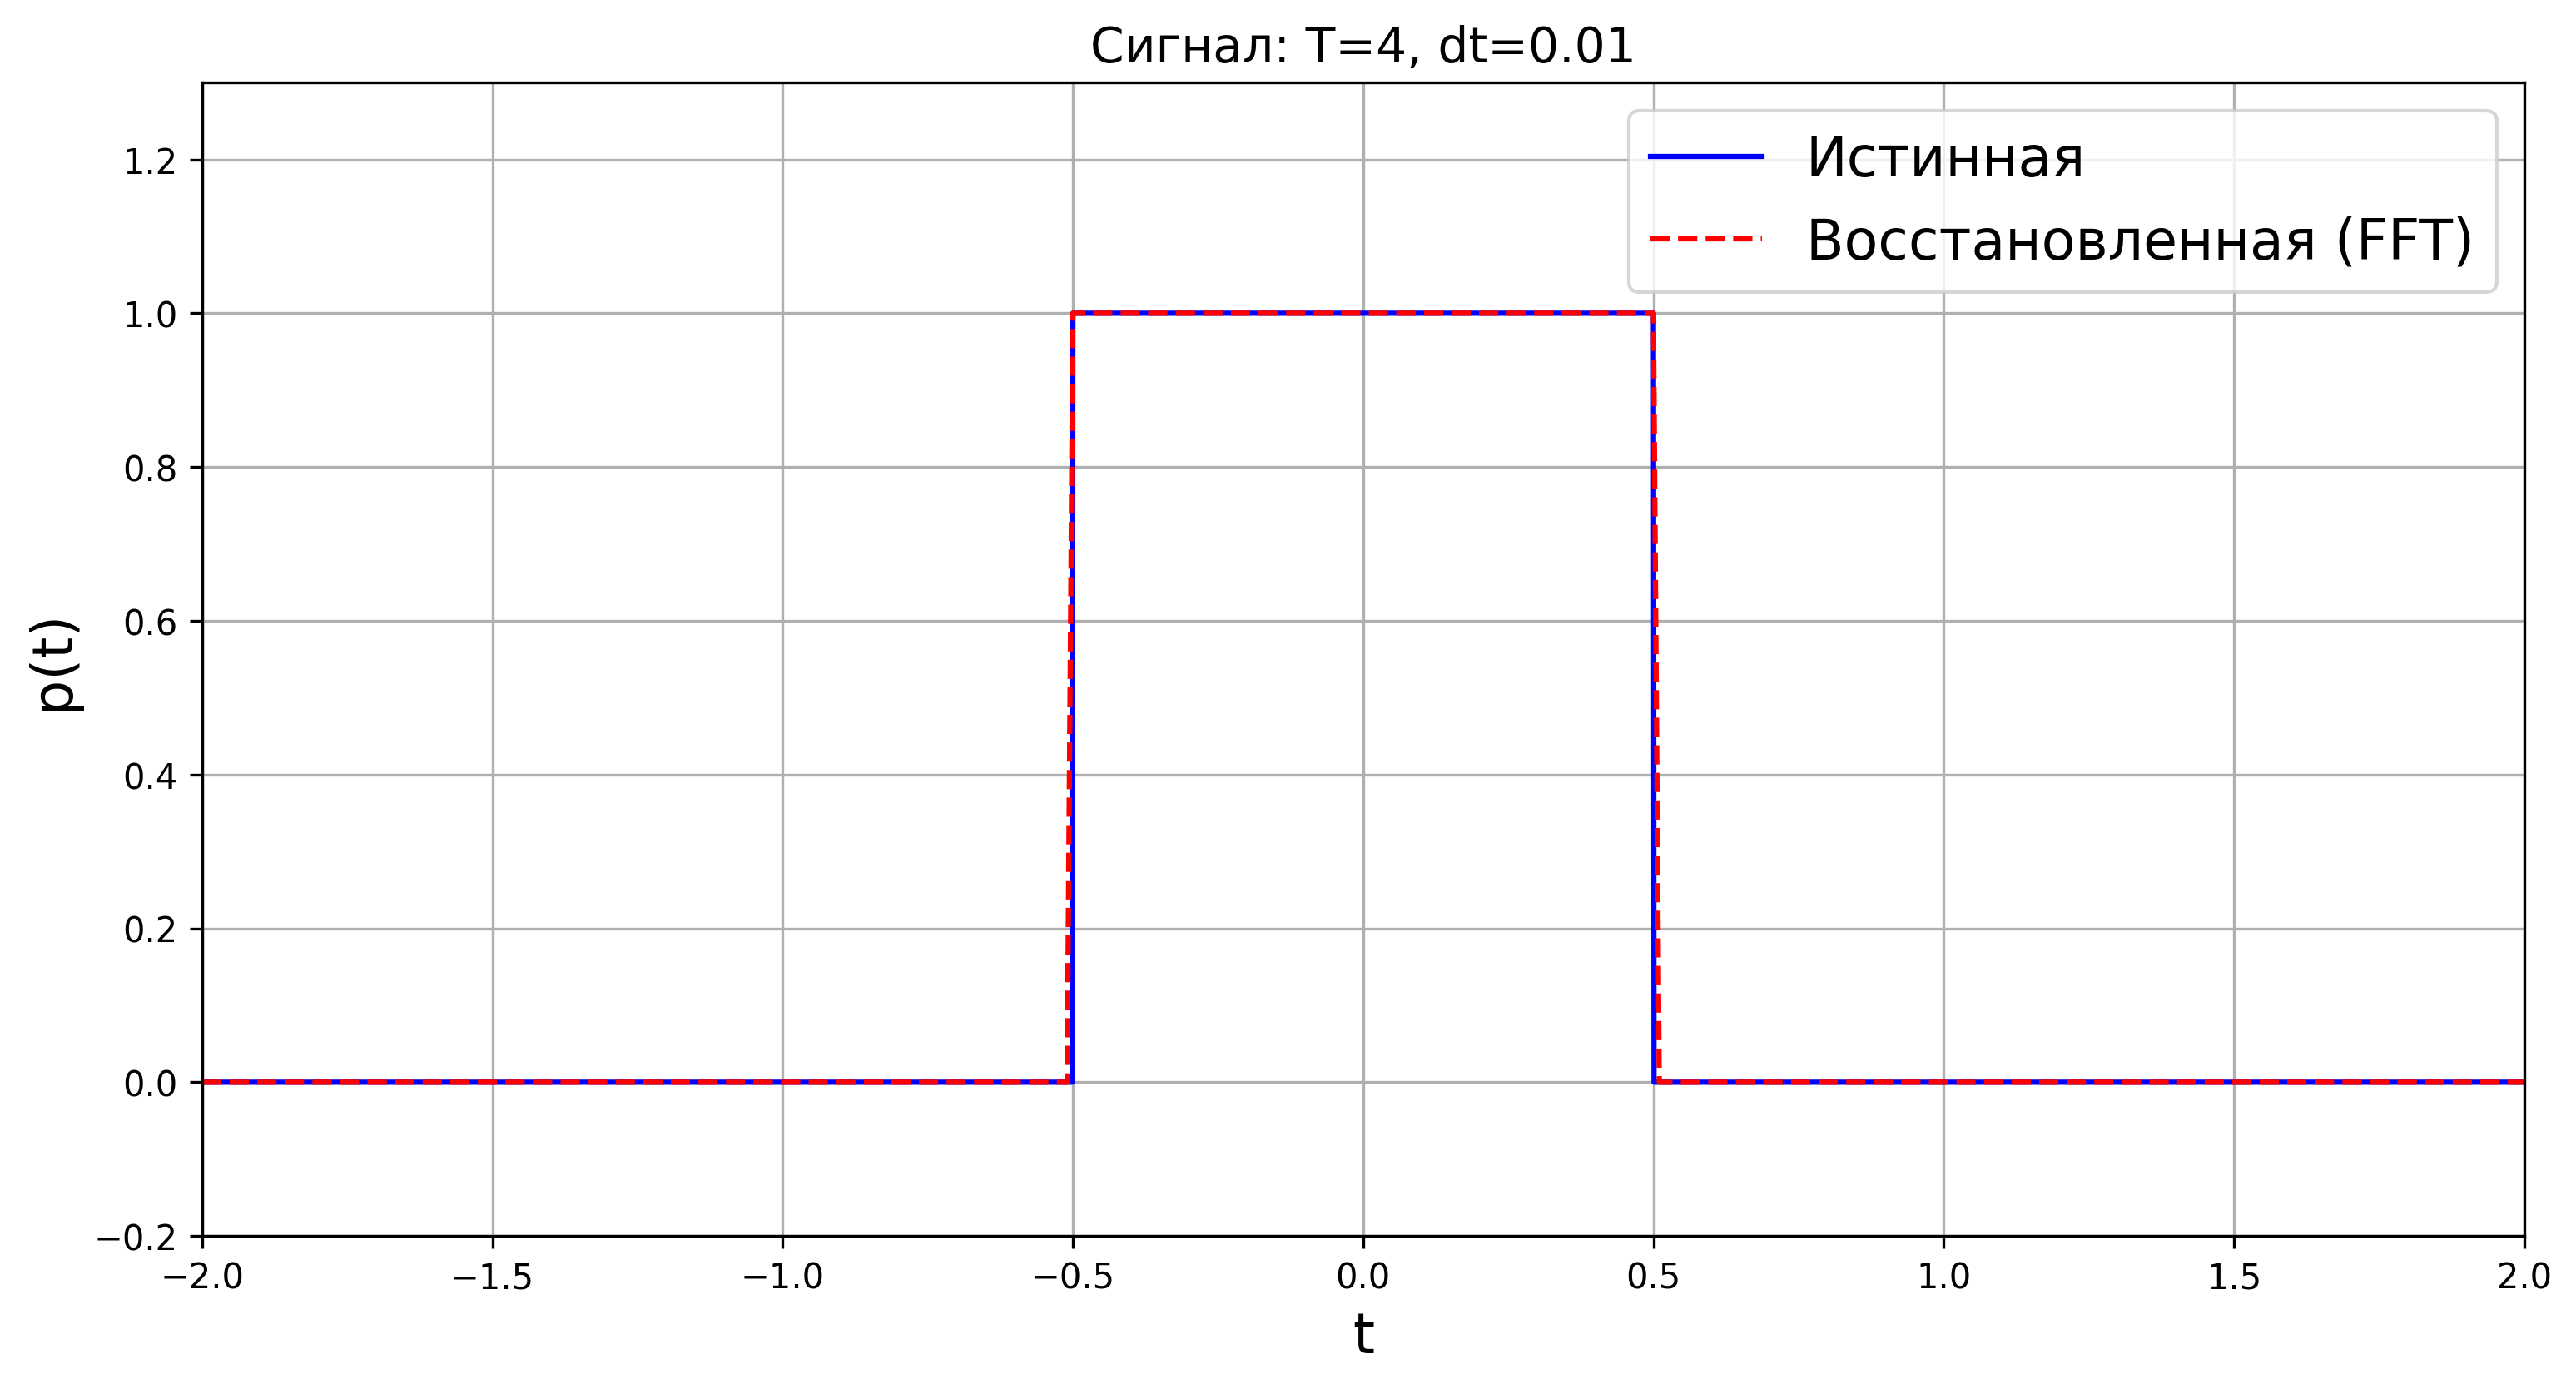
\includegraphics[width=0.95\textwidth]{images/FFT_T4_V200_dt0.010_dv0.100_signal.png}
    \caption{Восстановление сигнала: $T=4$, $dt=0.01$.}
\end{figure}

\begin{figure}[H]
    \centering
    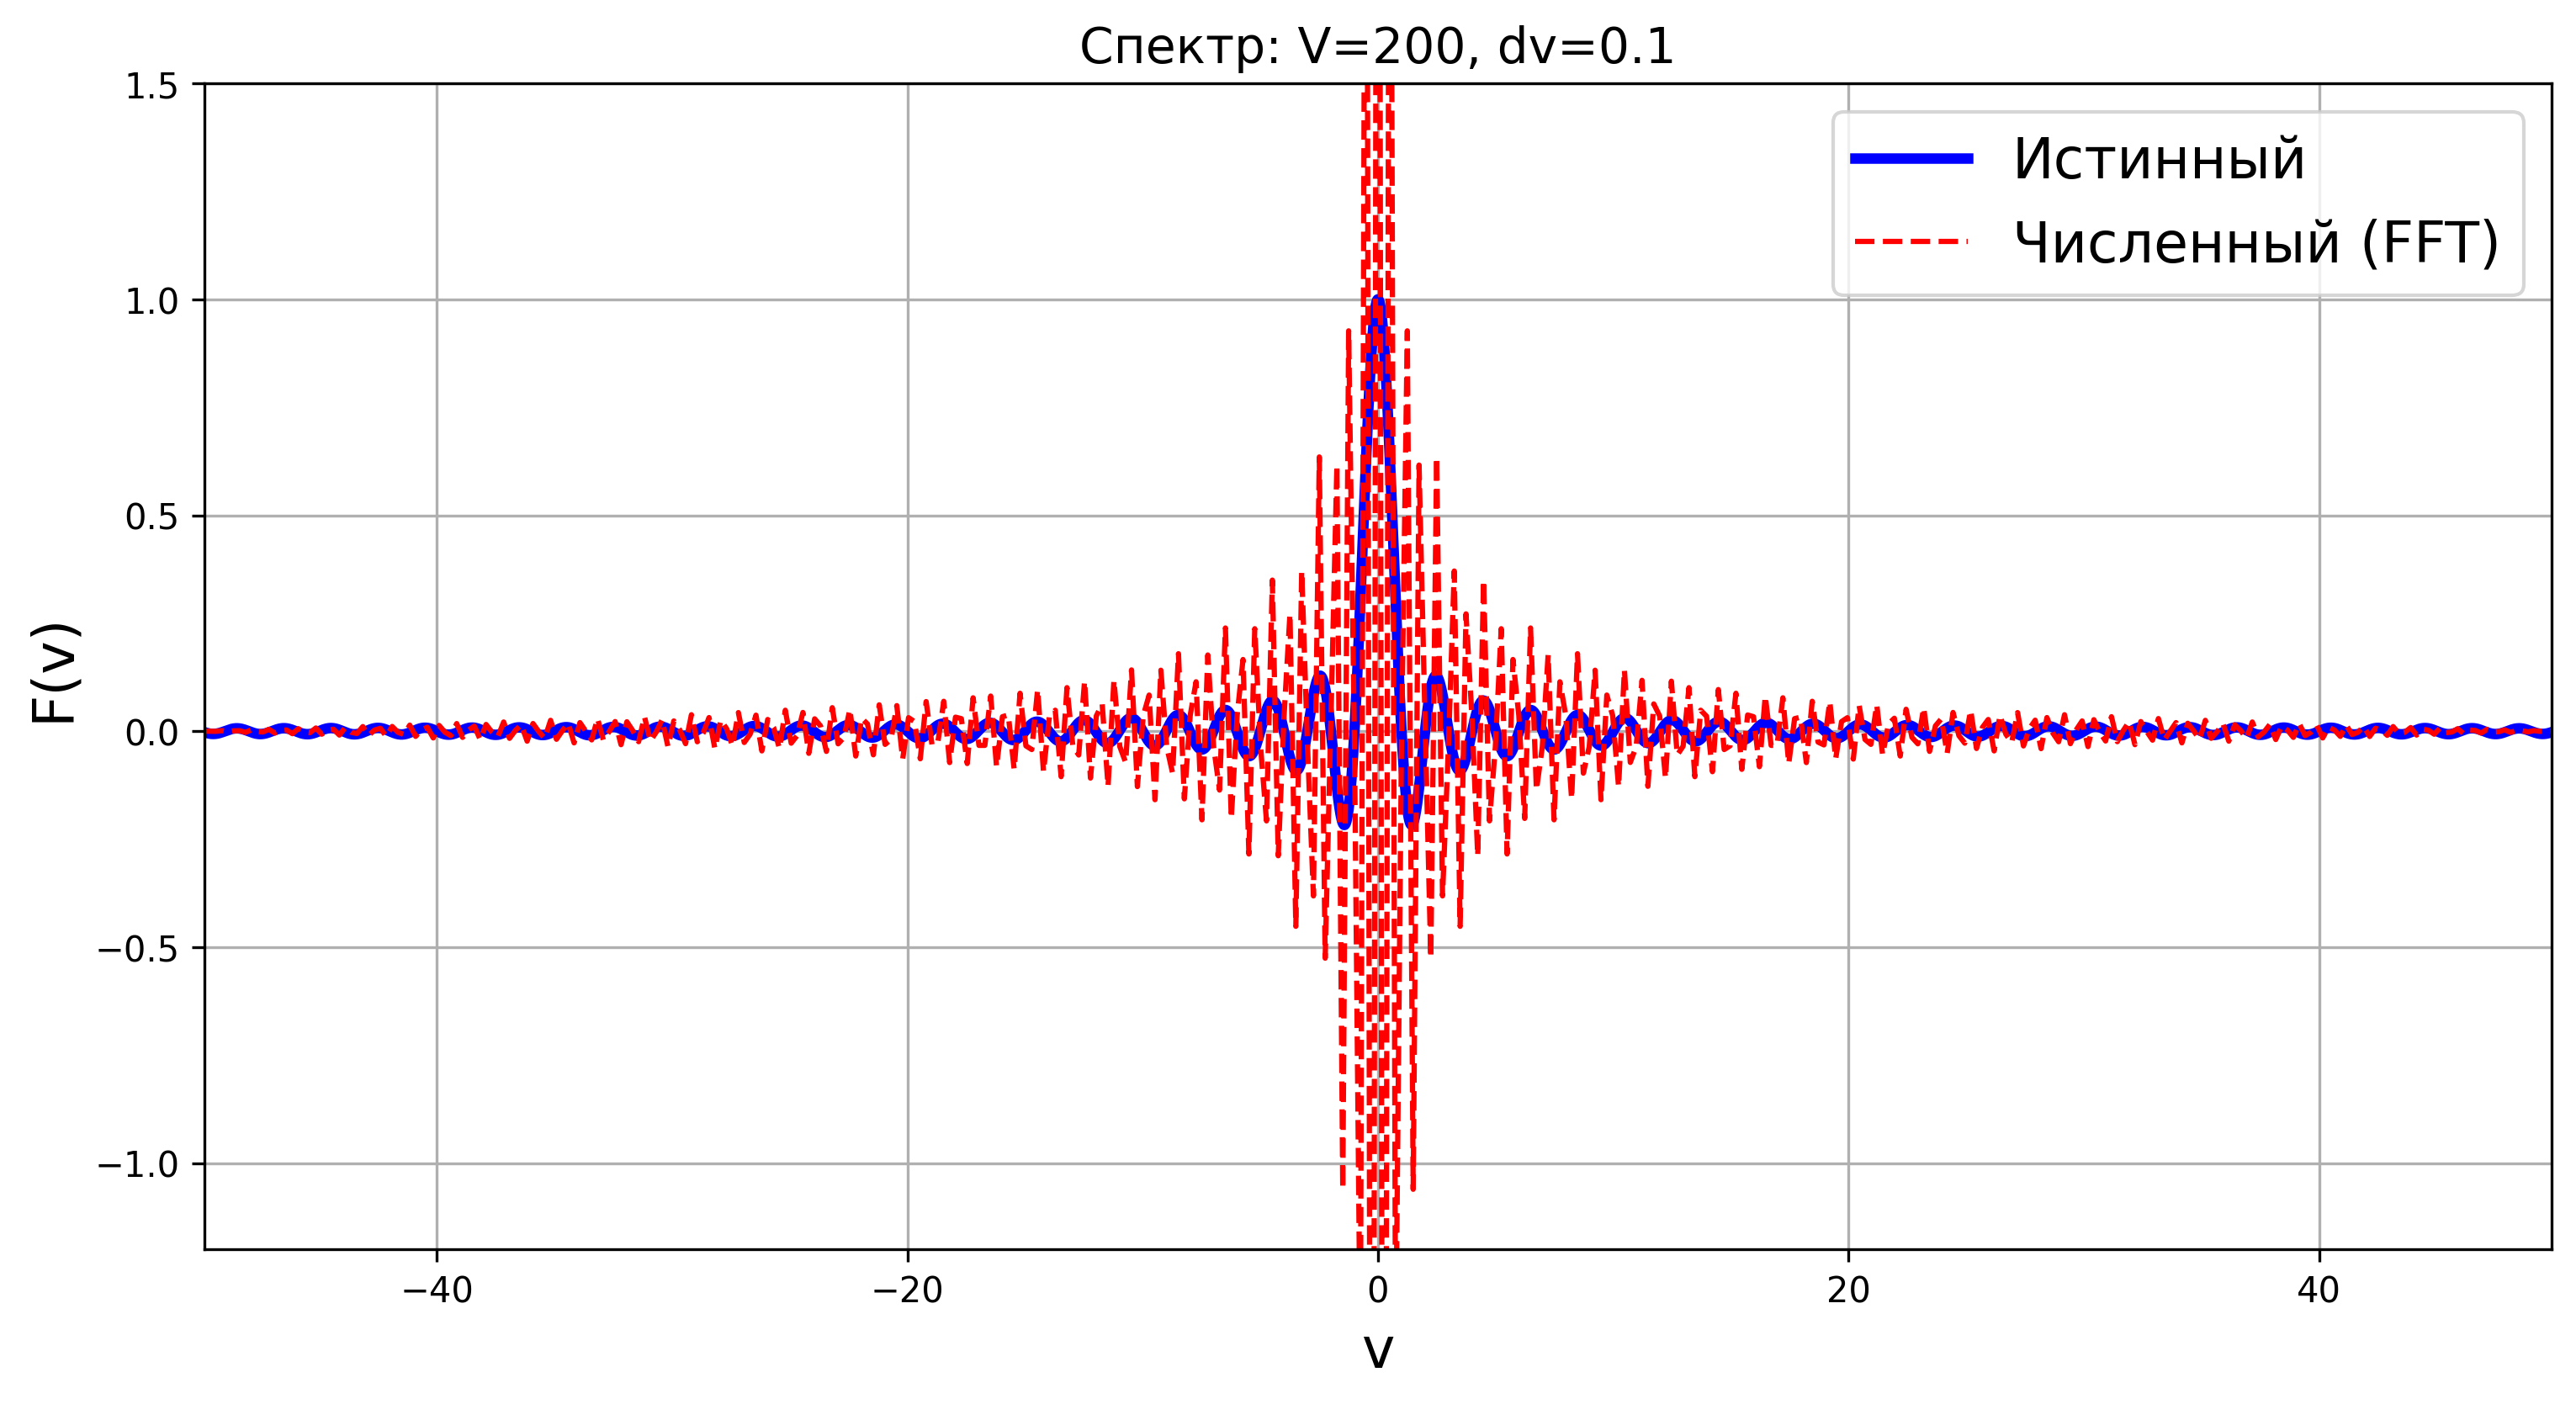
\includegraphics[width=0.95\textwidth]{images/FFT_T4_V200_dt0.010_dv0.100_spectrum.png}
    \caption{Сравнение спектров: $V=200$, $dv=0.1$.}
\end{figure}

\newpage
\subsection*{Комбинация 4: $T=4$, $V=100$, $dt=0.1$, $dv=0.1$}

\begin{figure}[H]
    \centering
    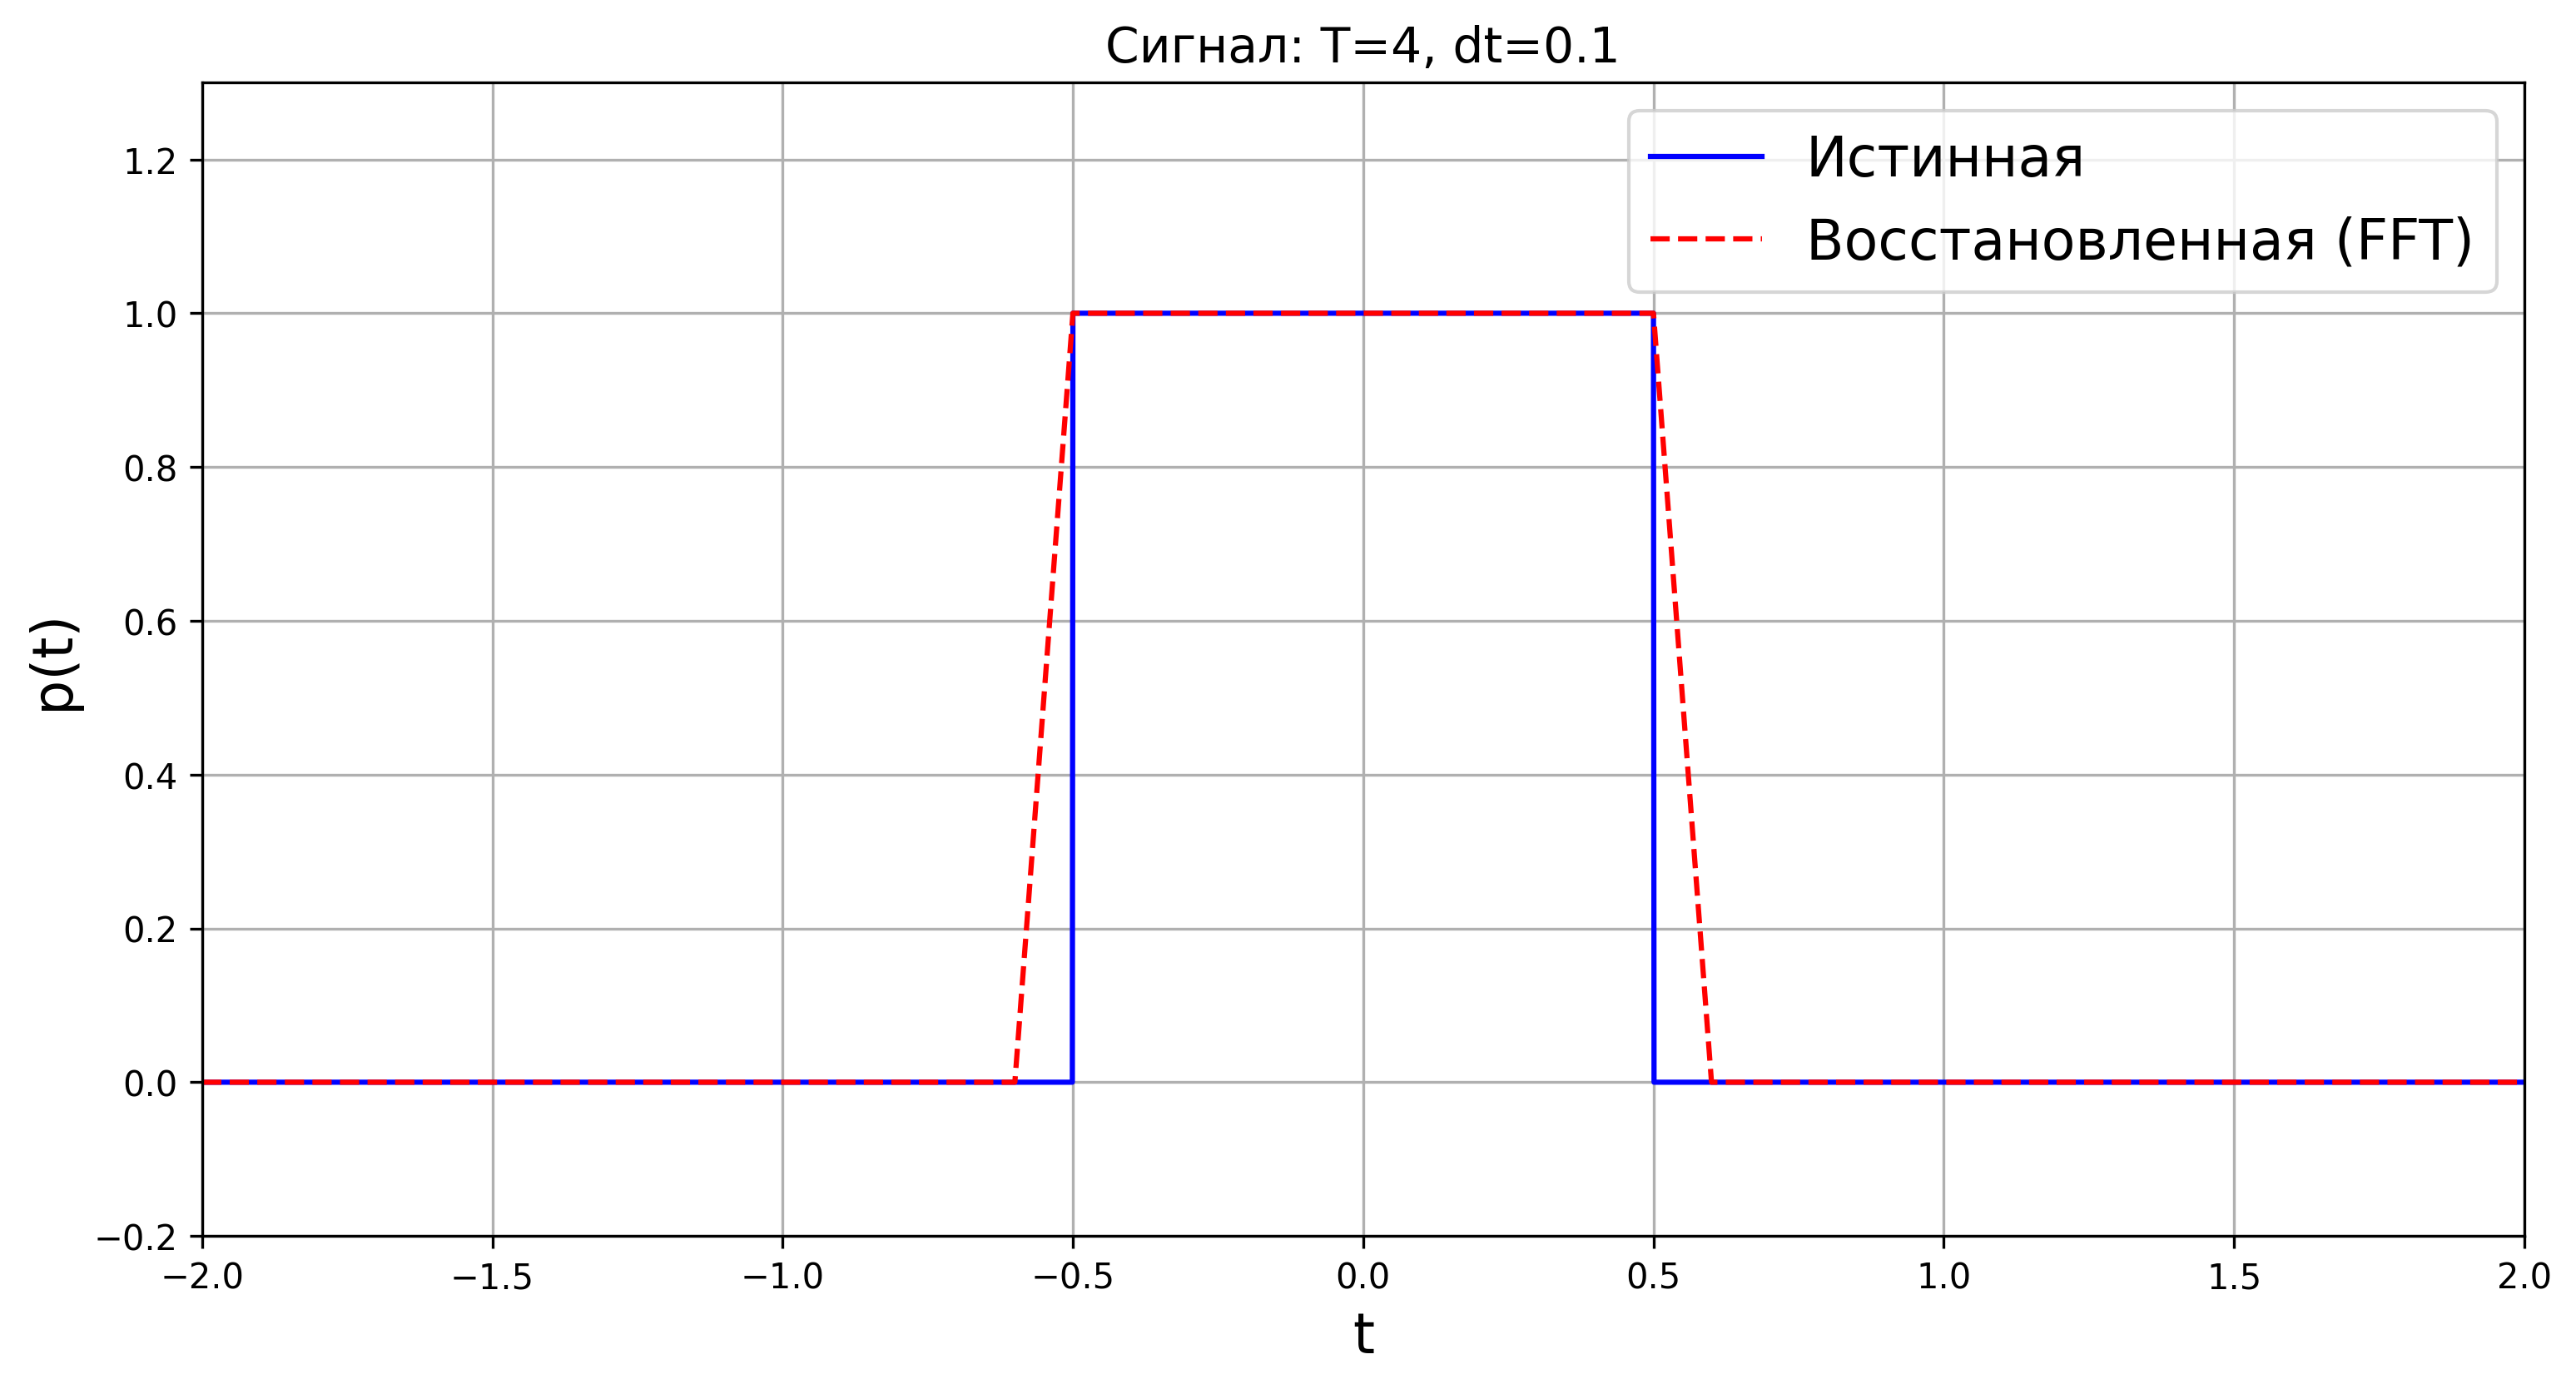
\includegraphics[width=0.95\textwidth]{images/FFT_T4_V100_dt0.100_dv0.100_signal.png}
    \caption{Восстановление сигнала: $T=4$, $dt=0.1$.}
\end{figure}

\begin{figure}[H]
    \centering
    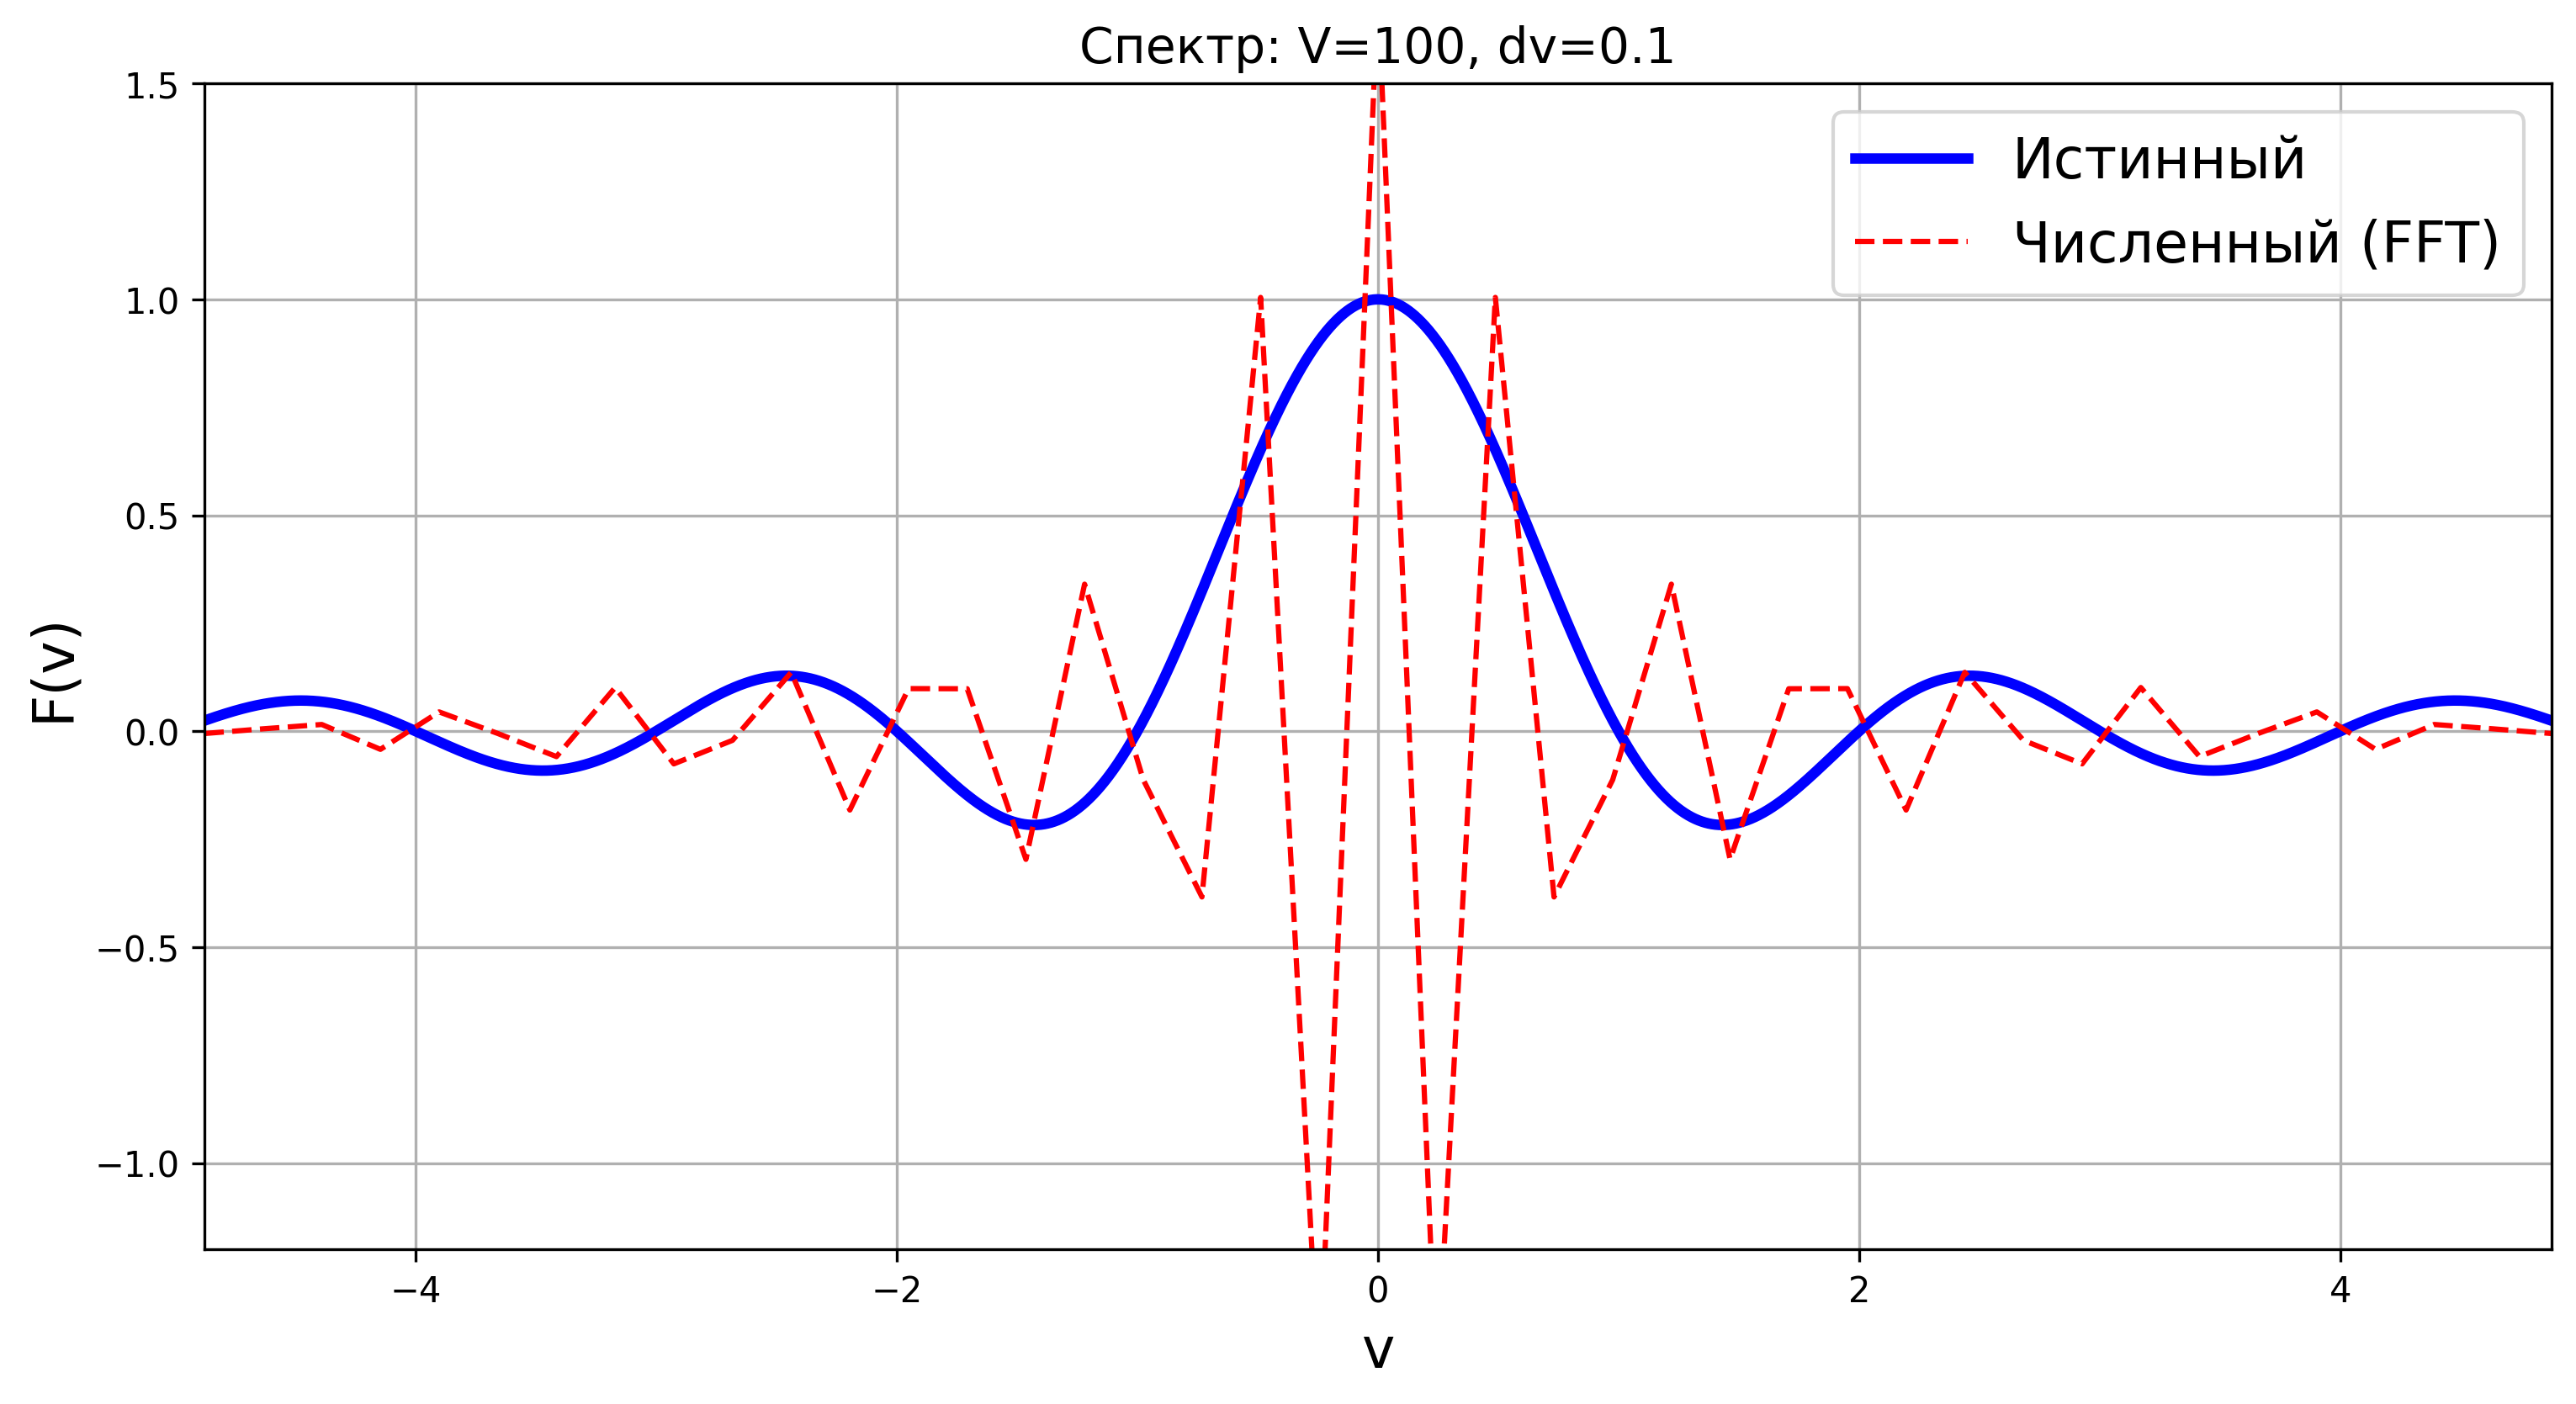
\includegraphics[width=0.95\textwidth]{images/FFT_T4_V100_dt0.100_dv0.100_spectrum.png}
    \caption{Сравнение спектров: $V=100$, $dv=0.1$.}
\end{figure}

\newpage
\subsection*{Комбинация 5: $T=4$, $V=100$, $dt=0.01$, $dv=0.5$}

\begin{figure}[H]
    \centering
    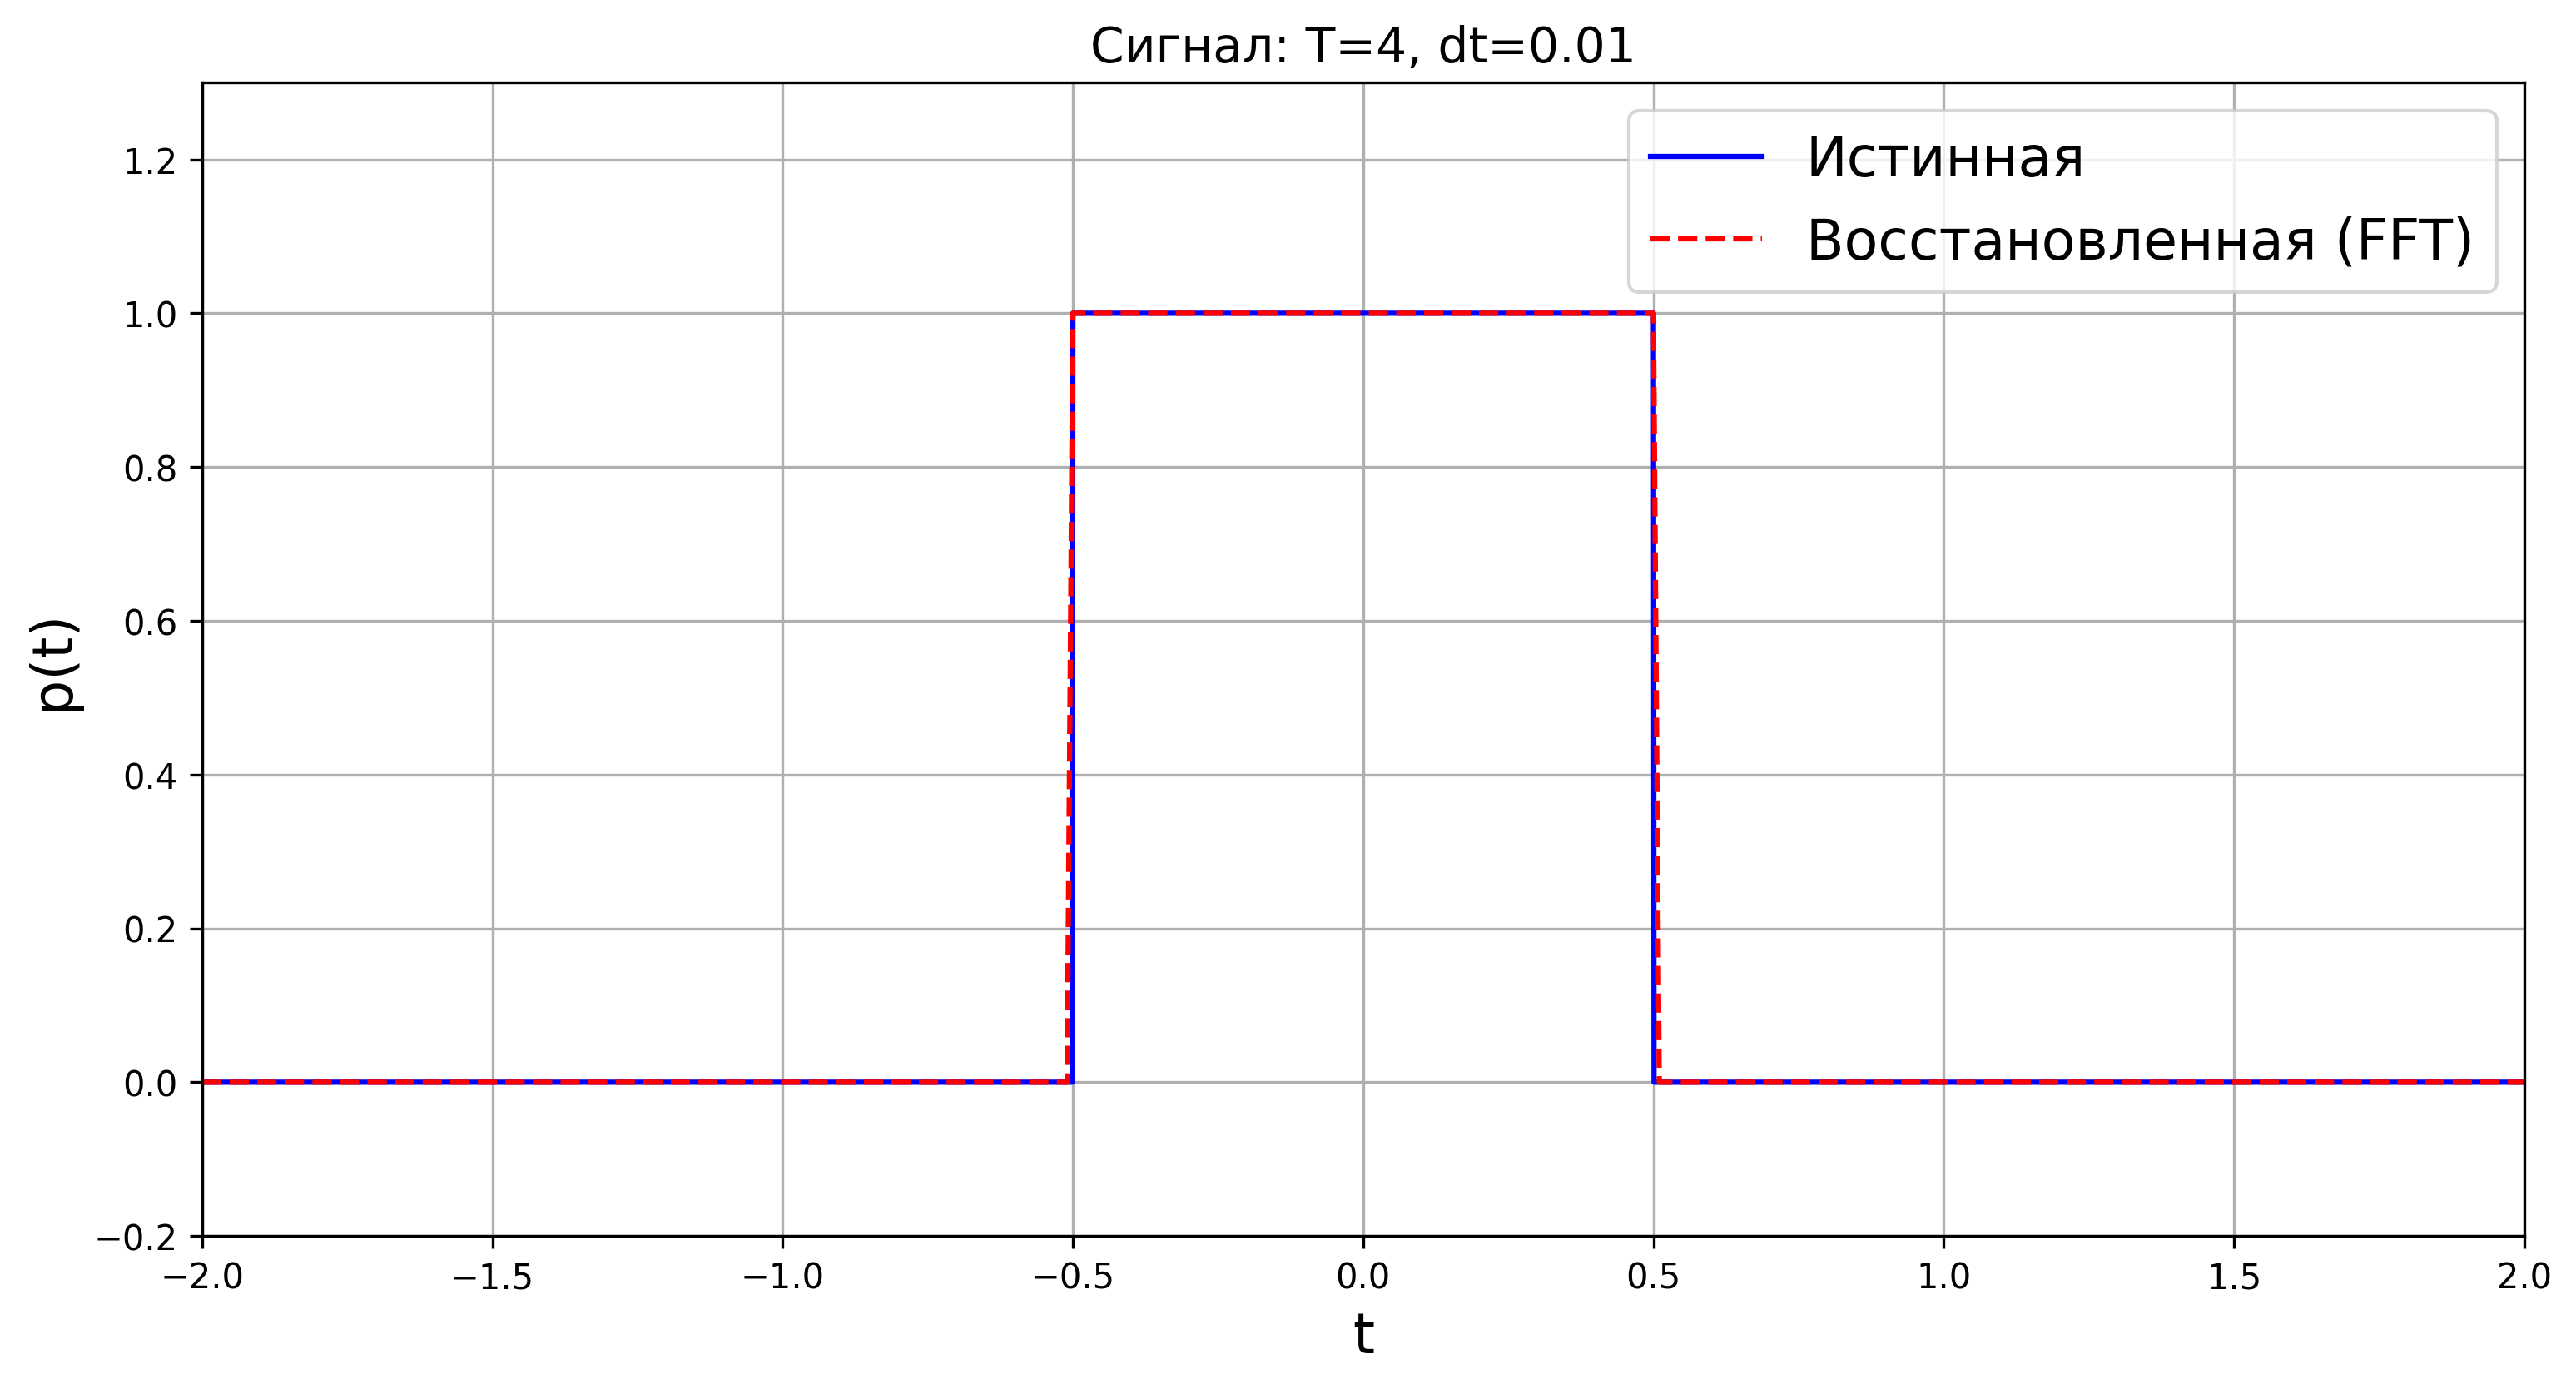
\includegraphics[width=0.95\textwidth]{images/FFT_T4_V100_dt0.010_dv0.500_signal.png}
    \caption{Восстановление сигнала: $T=4$, $dt=0.01$.}
\end{figure}

\begin{figure}[H]
    \centering
    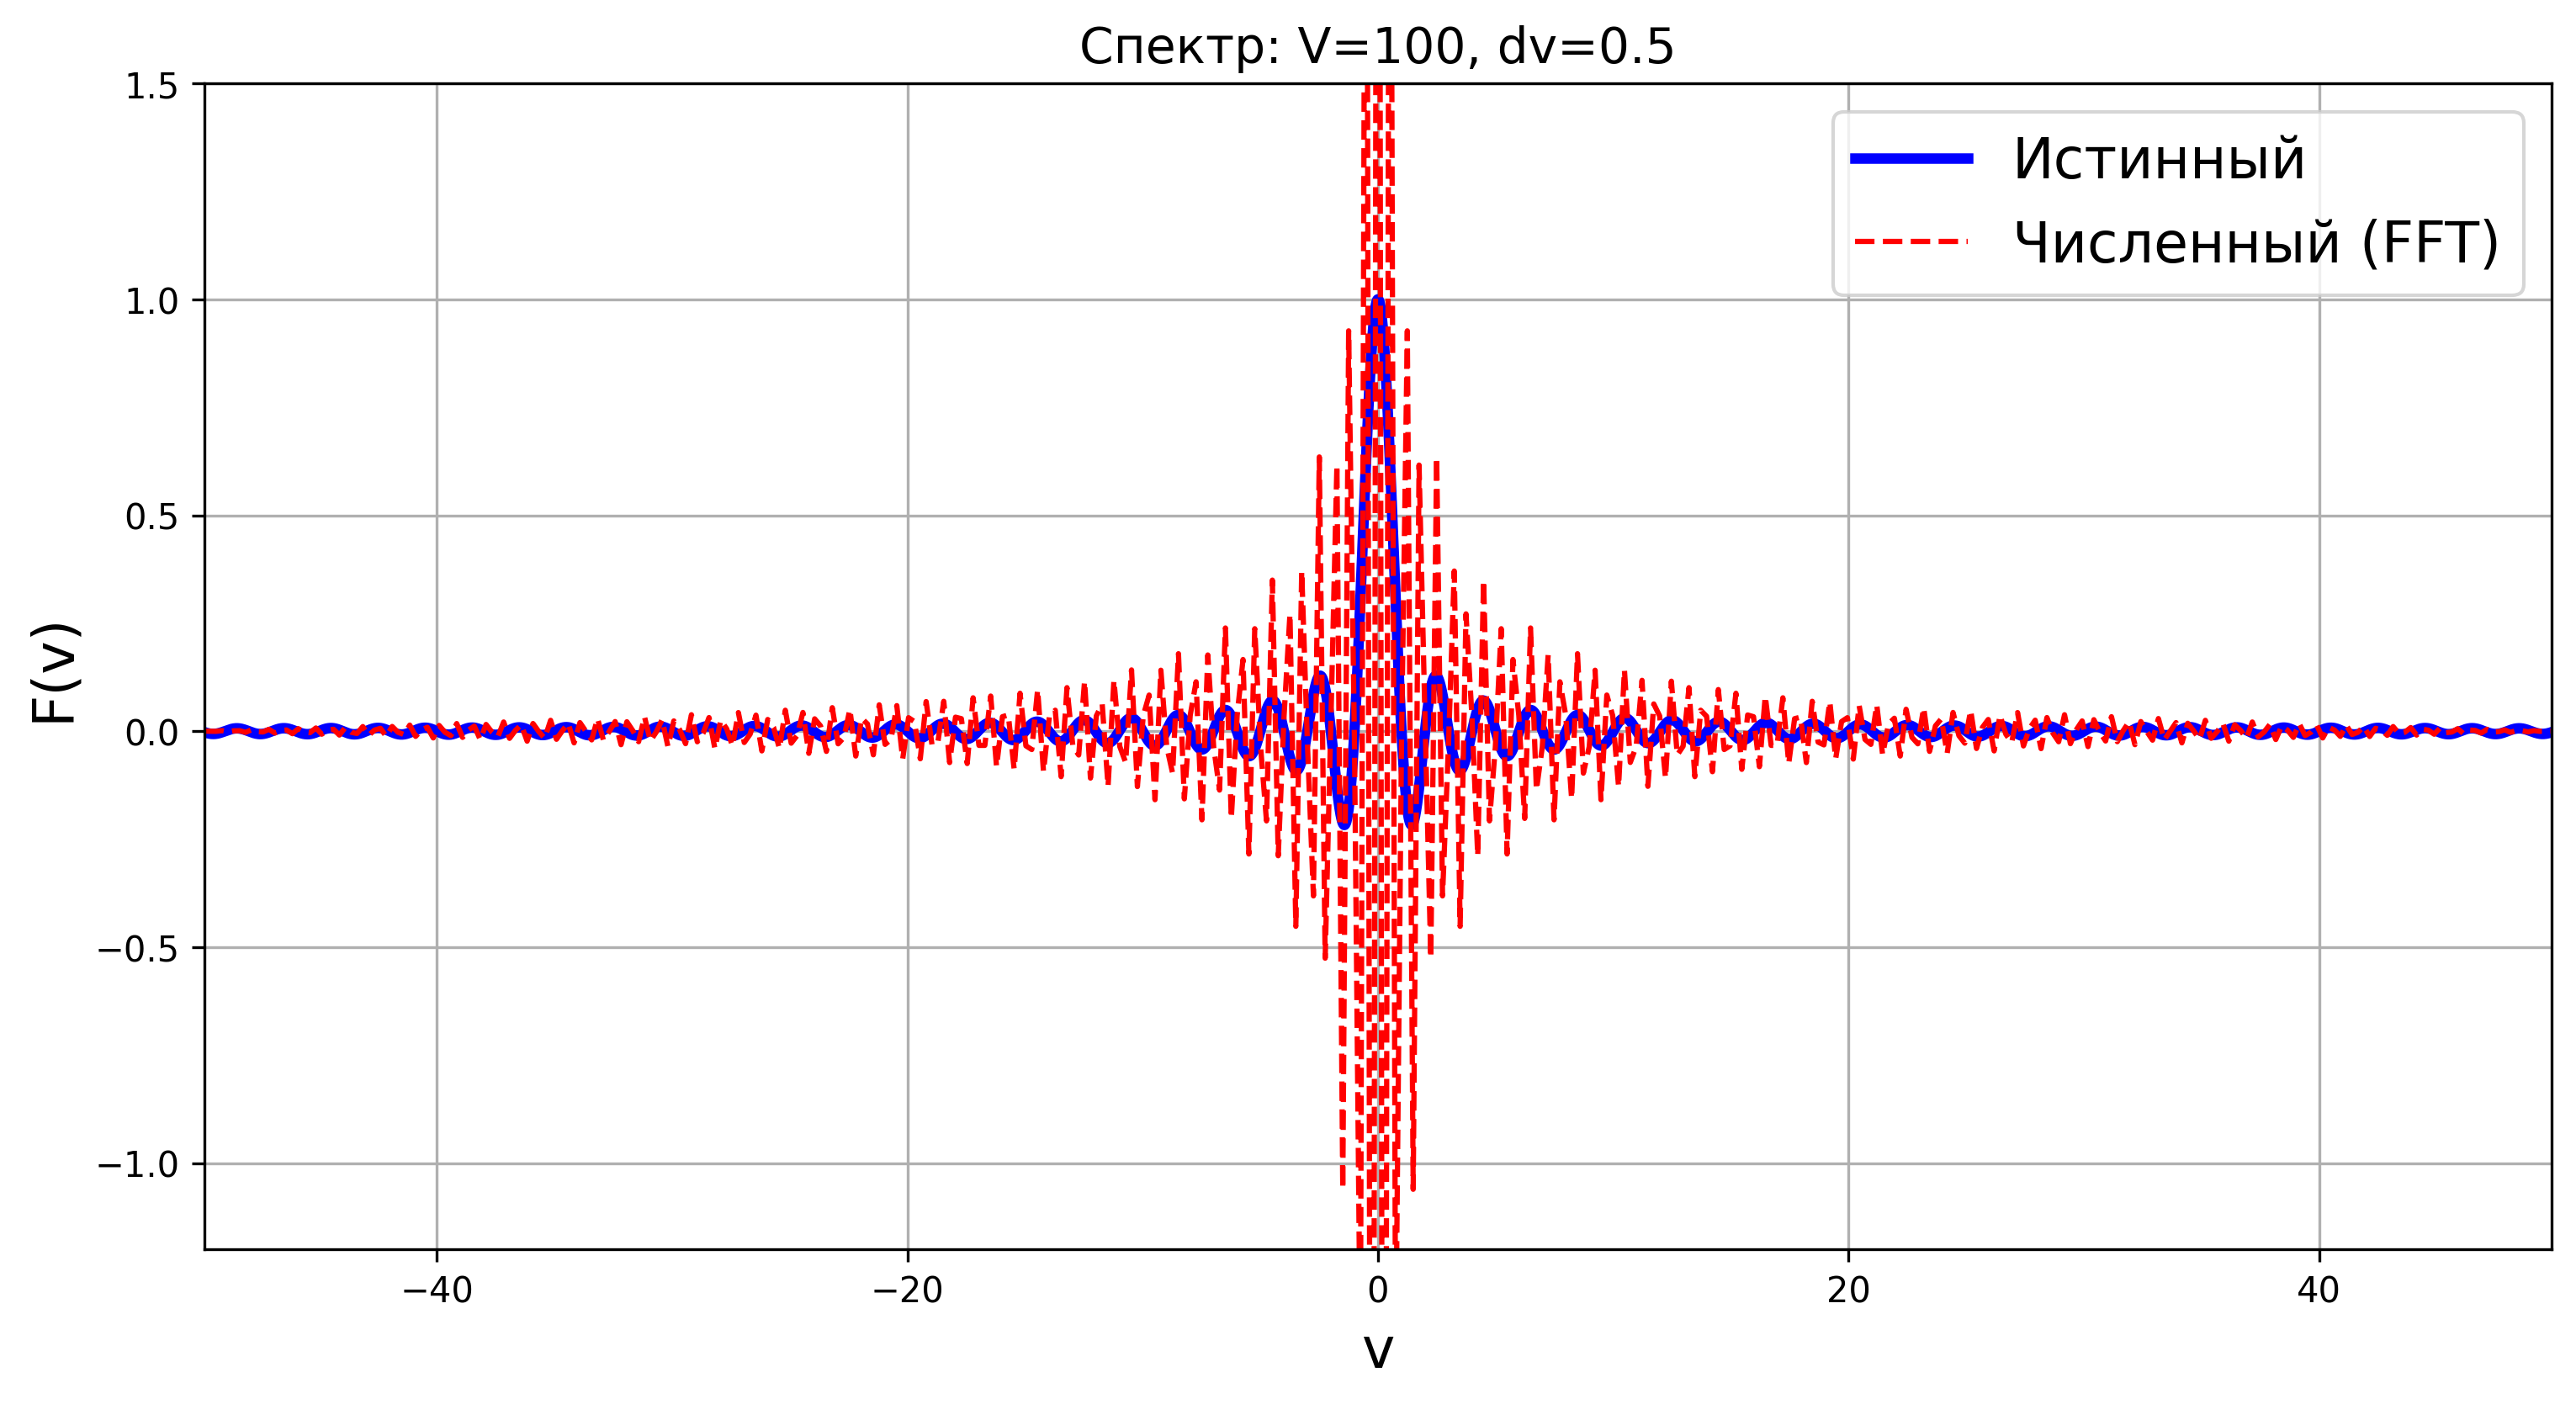
\includegraphics[width=0.95\textwidth]{images/FFT_T4_V100_dt0.010_dv0.500_spectrum.png}
    \caption{Сравнение спектров: $V=100$, $dv=0.5$.}
\end{figure}


\newpage
\subsection{Совмещение методов}

Итак, ввёдм константы $c_m$, которые выполняют функцию $\Delta t$.
Преобразование Фурье на интервале $[-T/2, T/2]$:
Сумма Римана:
\[
\int_a^b f(t)dt \approx \sum_{n=0}^{N-1} f(t_n)\Delta t, \quad \text{где } t_n = a + n\Delta t, \quad \Delta t = \frac{b-a}{N-1}
\]

Преобразование Фурье:
\[
\hat{f}(\nu) \approx \int_{-\frac{T}{2}}^{\frac{T}{2}} f(t)e^{-2\pi i \nu t}dt \to \hat{f}(\nu_m) \approx c_m \sum_{n=0}^{N-1} f(t_n)e^{-2\pi i \frac{nm}{N}}
\]


Применяем сумму Римана к интегралу Фурье на интервале $[-T/2, T/2]$:
\[
\hat{f}(\nu_m) = \int_{-T/2}^{T/2} f(t)e^{-2\pi i \nu_m t}dt \approx \sum_{n=0}^{N-1} f(t_n)e^{-2\pi i \nu_m t_n} \cdot \Delta t
\]


Определяем положение точек дискретизации. Для симметричного интервала $[-T/2, T/2]$ точки должны располагаться симметрично относительно нуля:
\[
t_n = \left(n - \frac{N-1}{2}\right)\Delta t = \left(n - \frac{N-1}{2}\right)\frac{T}{N}, \quad n = 0, 1, \ldots, N-1
\]

Подставляем $t_n$ и $\nu_m$ в экспоненту:
\[
e^{-2\pi i \nu_m t_n} = e^{-2\pi i \cdot \frac{m}{T} \cdot \left(n - \frac{N-1}{2}\right) \cdot \frac{T}{N}} = e^{-2\pi i \cdot \frac{m}{T} \cdot \frac{T}{N} \cdot \left(n - \frac{N-1}{2}\right)} 
\]
\[
= e^{-2\pi i \frac{m}{N} \left(n - \frac{N-1}{2}\right)} = e^{-2\pi i \frac{mn}{N} + 2\pi i \frac{m(N-1)}{2N}}
\]
\[
= e^{-2\pi i \frac{mn}{N}} \cdot e^{\pi i m \frac{N-1}{N}} = e^{-2\pi i \frac{mn}{N}} \cdot e^{\pi i m \left(1 - \frac{1}{N}\right)}
\]
\[= e^{-2\pi i \frac{mn}{N}} \cdot e^{\pi i m} \cdot e^{-\pi i m/N} = e^{-2\pi i \frac{mn}{N}} \cdot (-1)^m \cdot e^{-\pi i m/N}
\]

Подставляем полученное выражение в сумму Римана:
\[
\hat{f}(\nu_m) \approx \sum_{n=0}^{N-1} f(t_n) \cdot e^{-2\pi i \frac{mn}{N}} \cdot (-1)^m \cdot e^{-\pi i m/N} \cdot \Delta t = (-1)^m \cdot e^{-\pi i m/N} \cdot \Delta t \cdot \sum_{n=0}^{N-1} f(t_n) e^{-2\pi i \frac{mn}{N}}
\]

Сравниваем с формулой:
\[
\hat{f}(\nu_m) \approx c_m \sum_{n=0}^{N-1} f(t_n)e^{-2\pi i \frac{nm}{N}}
\]
Отсюда получаем:
\[
c_m = (-1)^m \cdot e^{-\pi i m/N} \cdot \Delta t
\]

Рассмотрим различные комбинации параметров
\newpage
\subsection*{Комбинация 1: $T=4$, $V=100$, $dt=0.01$, $dv=0.1$}

\begin{figure}[H]
    \centering
    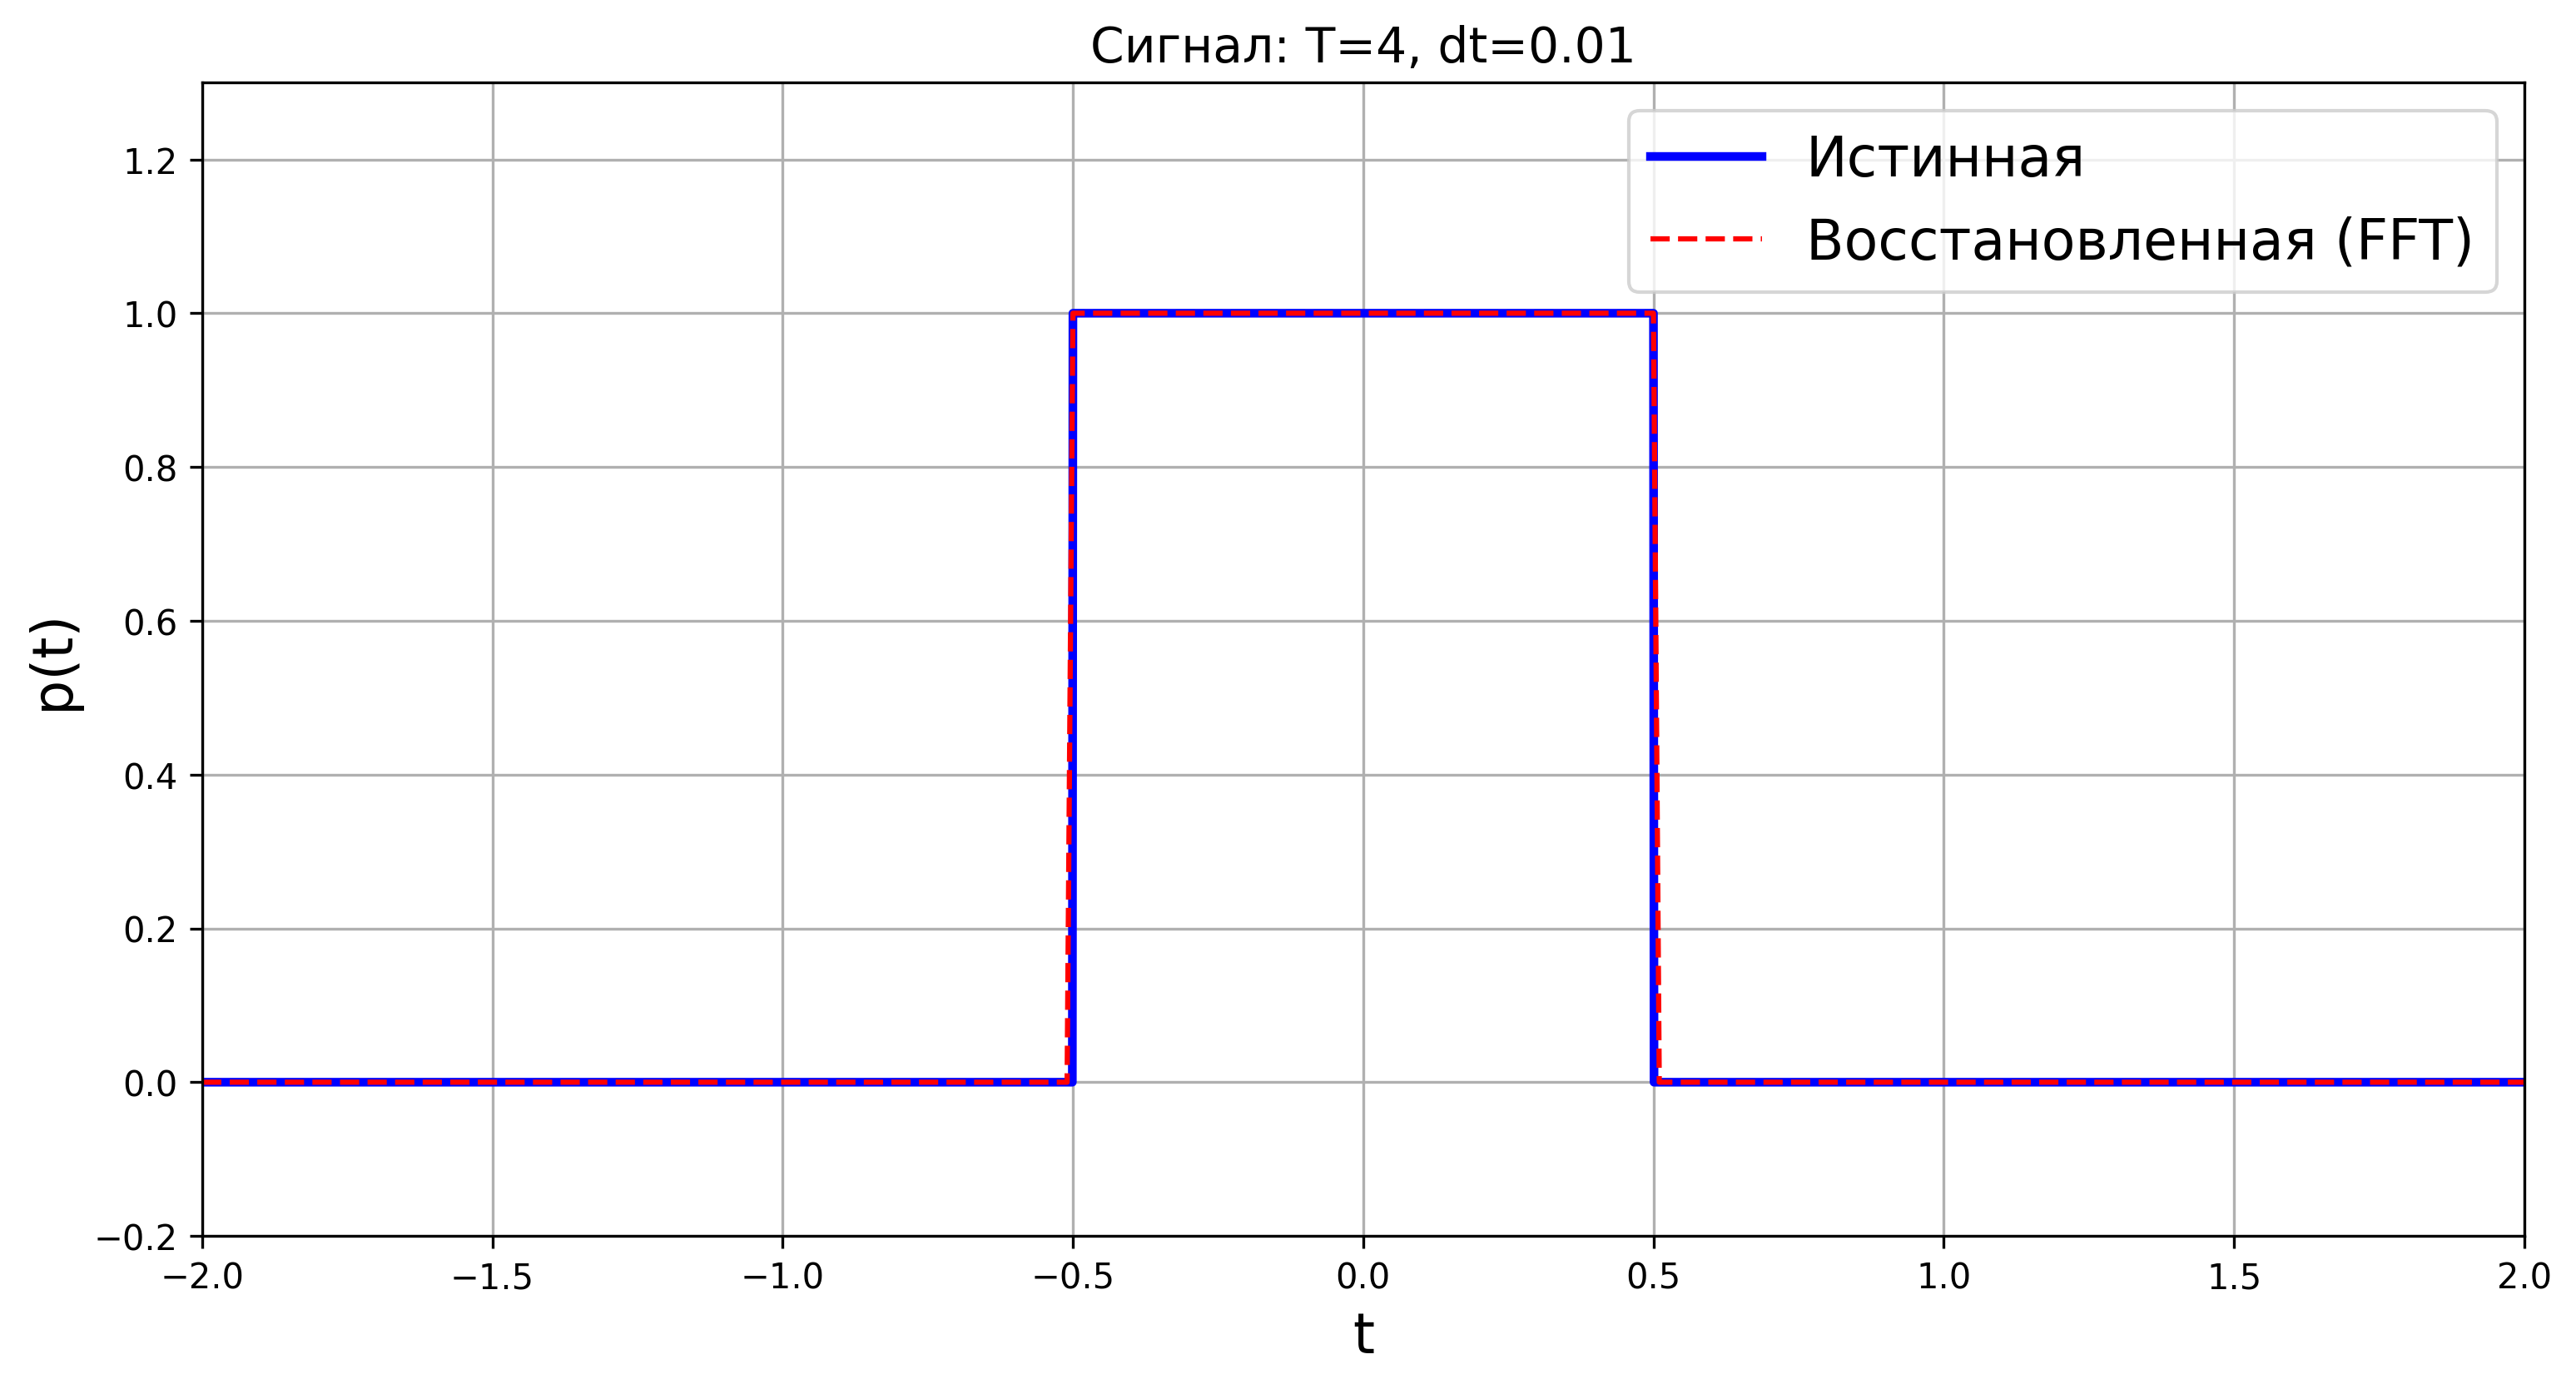
\includegraphics[width=0.95\textwidth]{images/FFTc_T4_V100_dt0.010_dv0.100_signal.png}
    \caption{Восстановление сигнала: $T=4$, $dt=0.01$.}
\end{figure}

\begin{figure}[H]
    \centering
    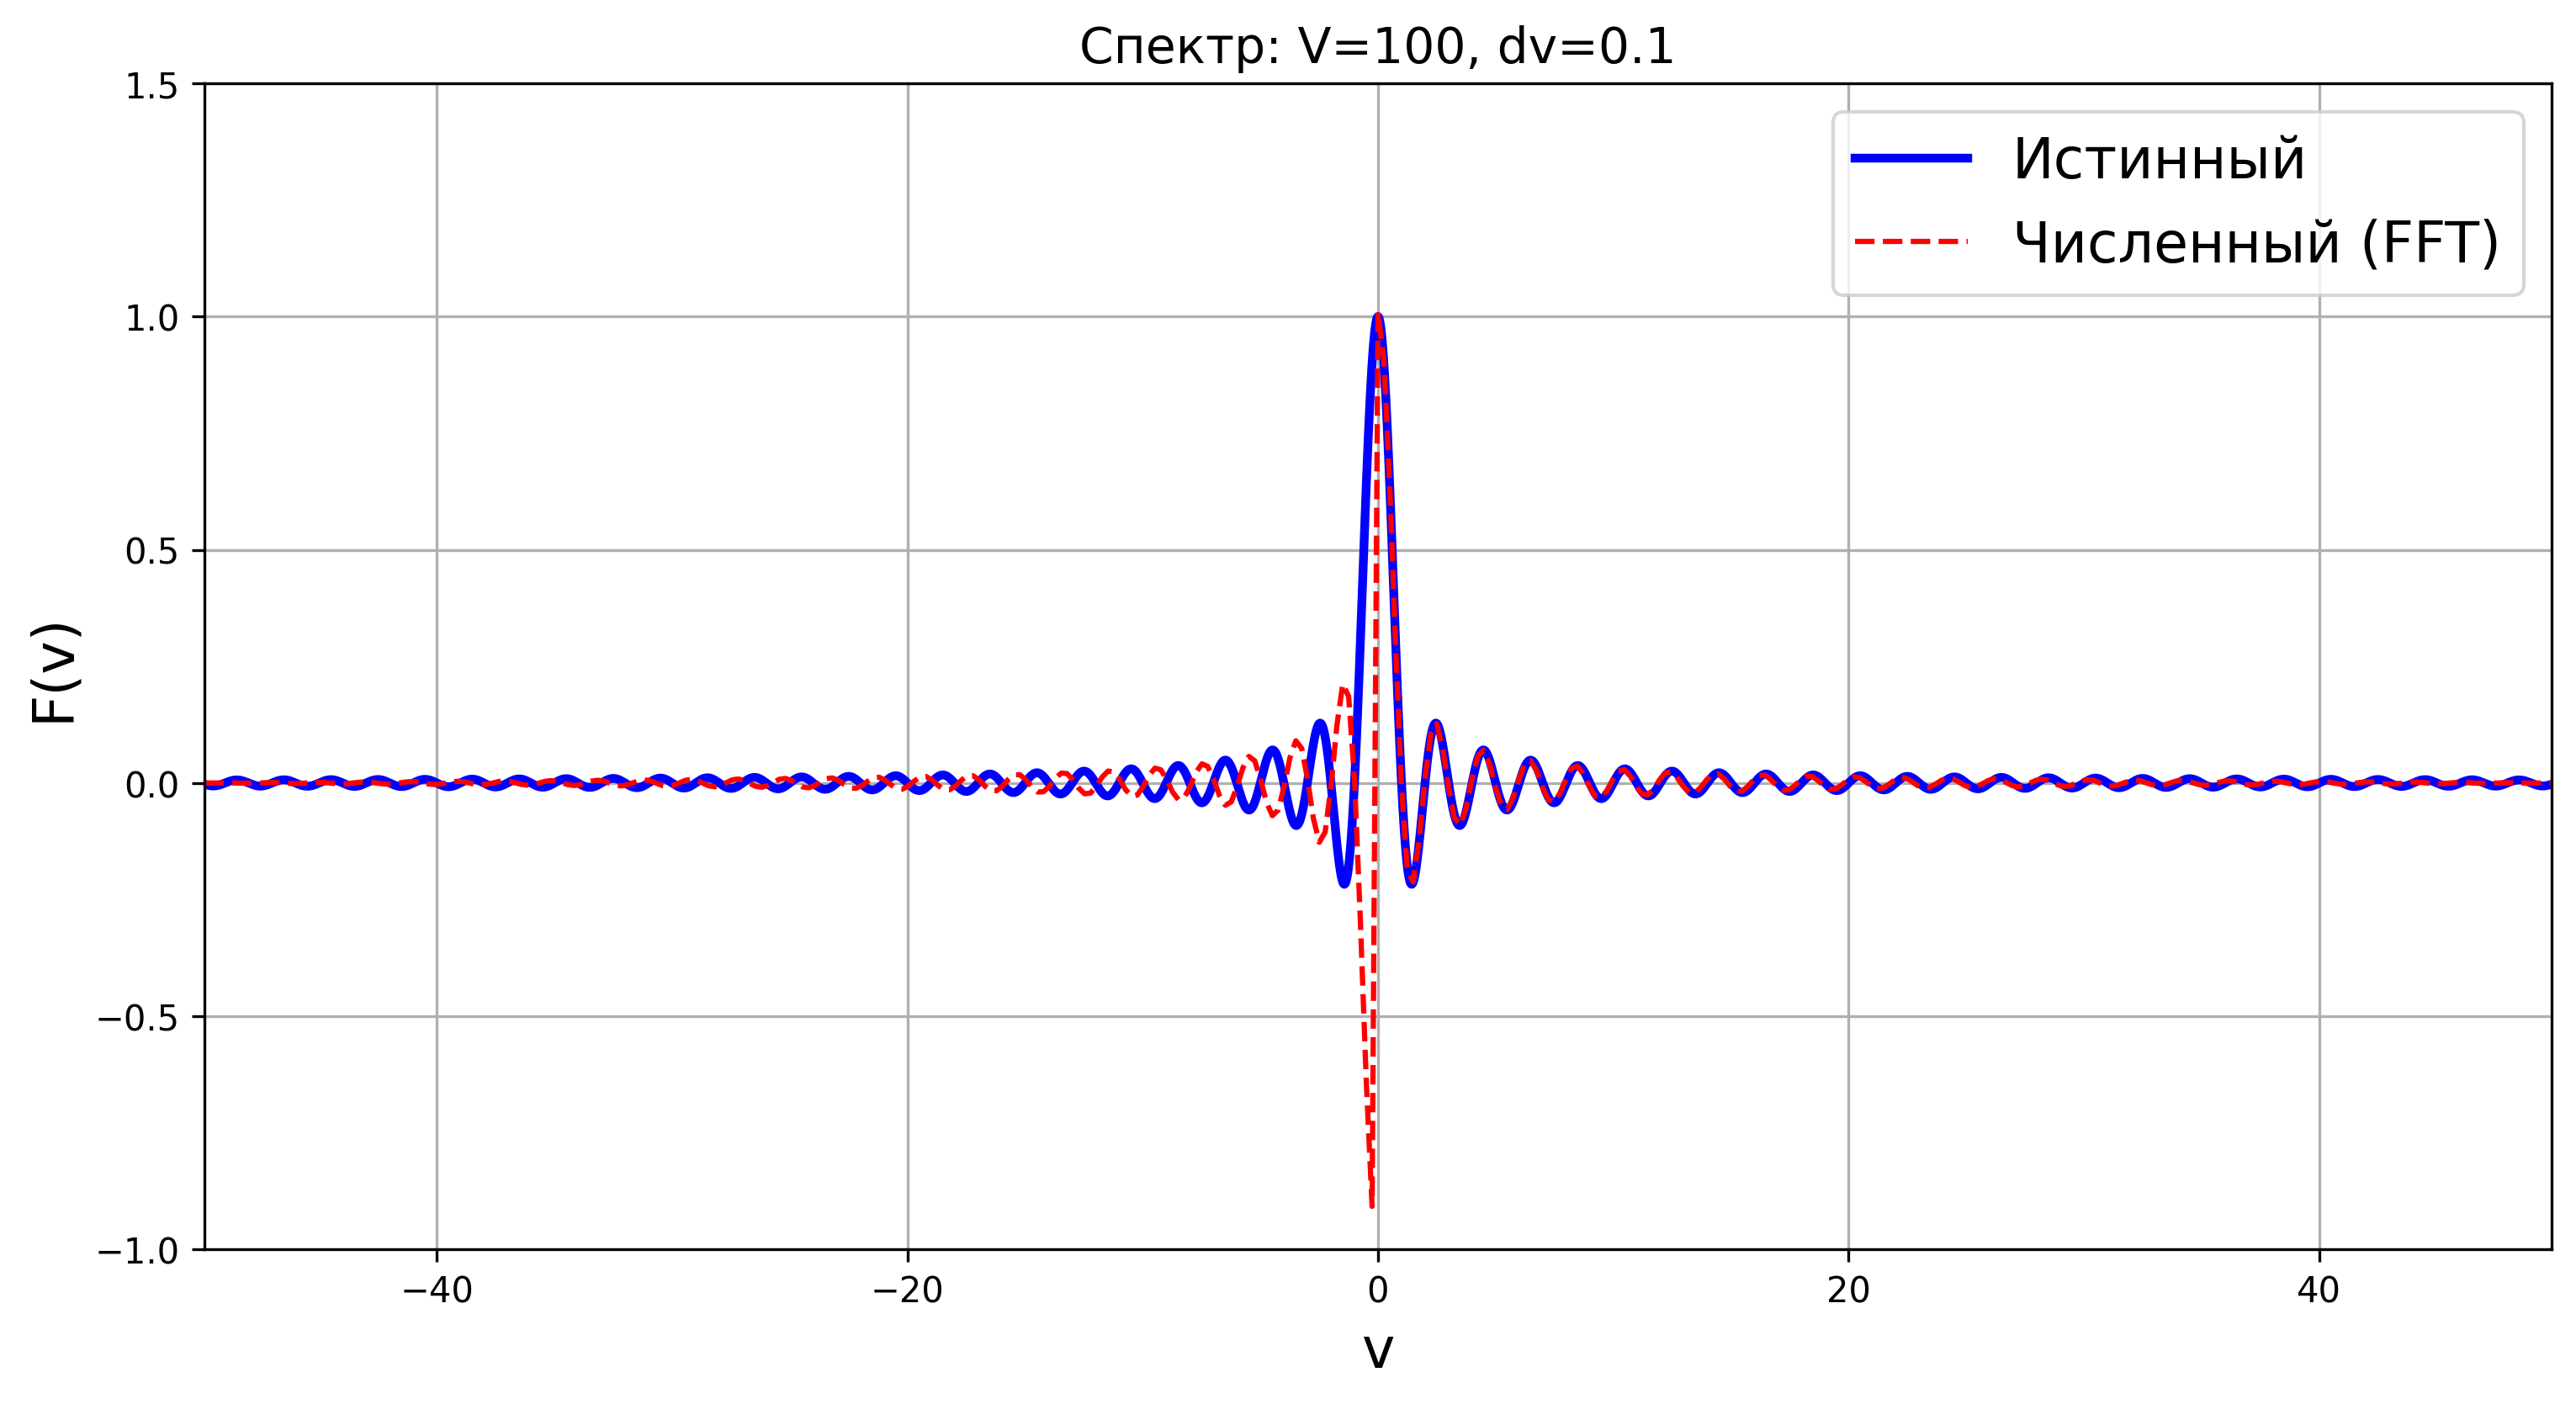
\includegraphics[width=0.95\textwidth]{images/FFTc_T4_V100_dt0.010_dv0.100_spectrum.png}
    \caption{Сравнение спектров: $V=100$, $dv=0.1$.}
\end{figure}

\newpage
\subsection*{Комбинация 2: $T=15$, $V=100$, $dt=0.01$, $dv=0.1$}

\begin{figure}[H]
    \centering
    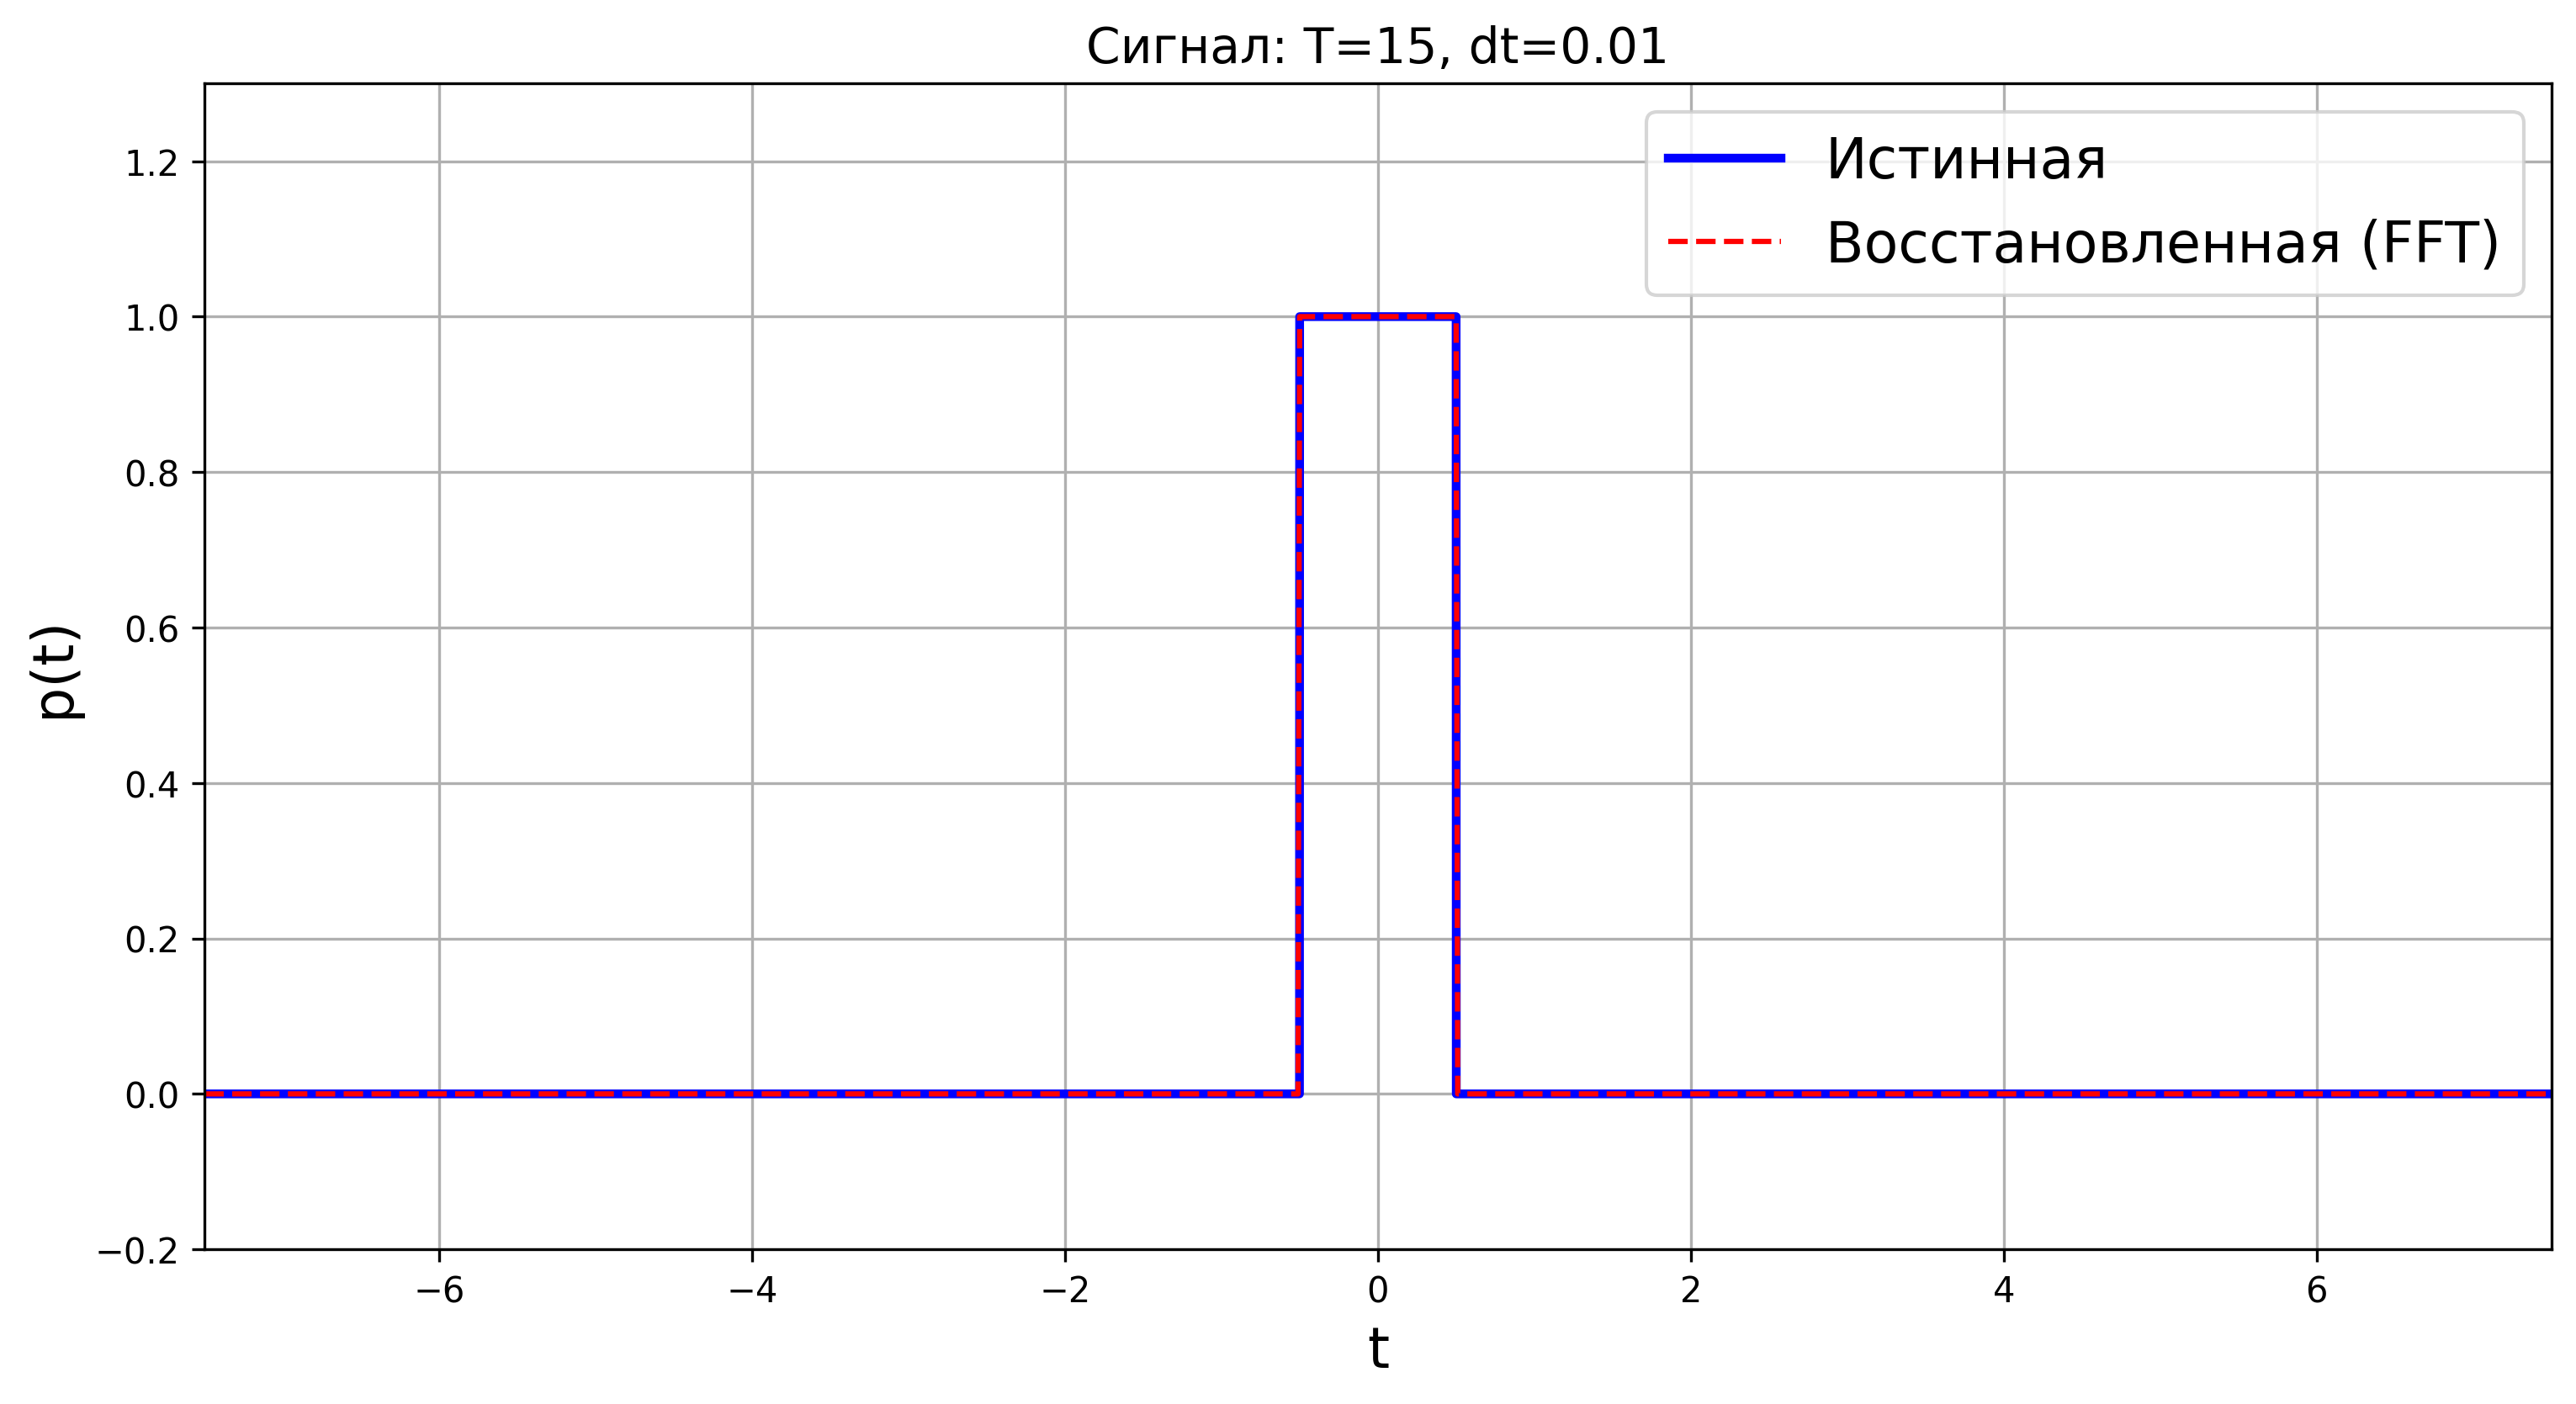
\includegraphics[width=0.95\textwidth]{images/FFTc_T15_V100_dt0.010_dv0.100_signal.png}
    \caption{Восстановление сигнала: $T=15$, $dt=0.01$.}
\end{figure}

\begin{figure}[H]
    \centering
    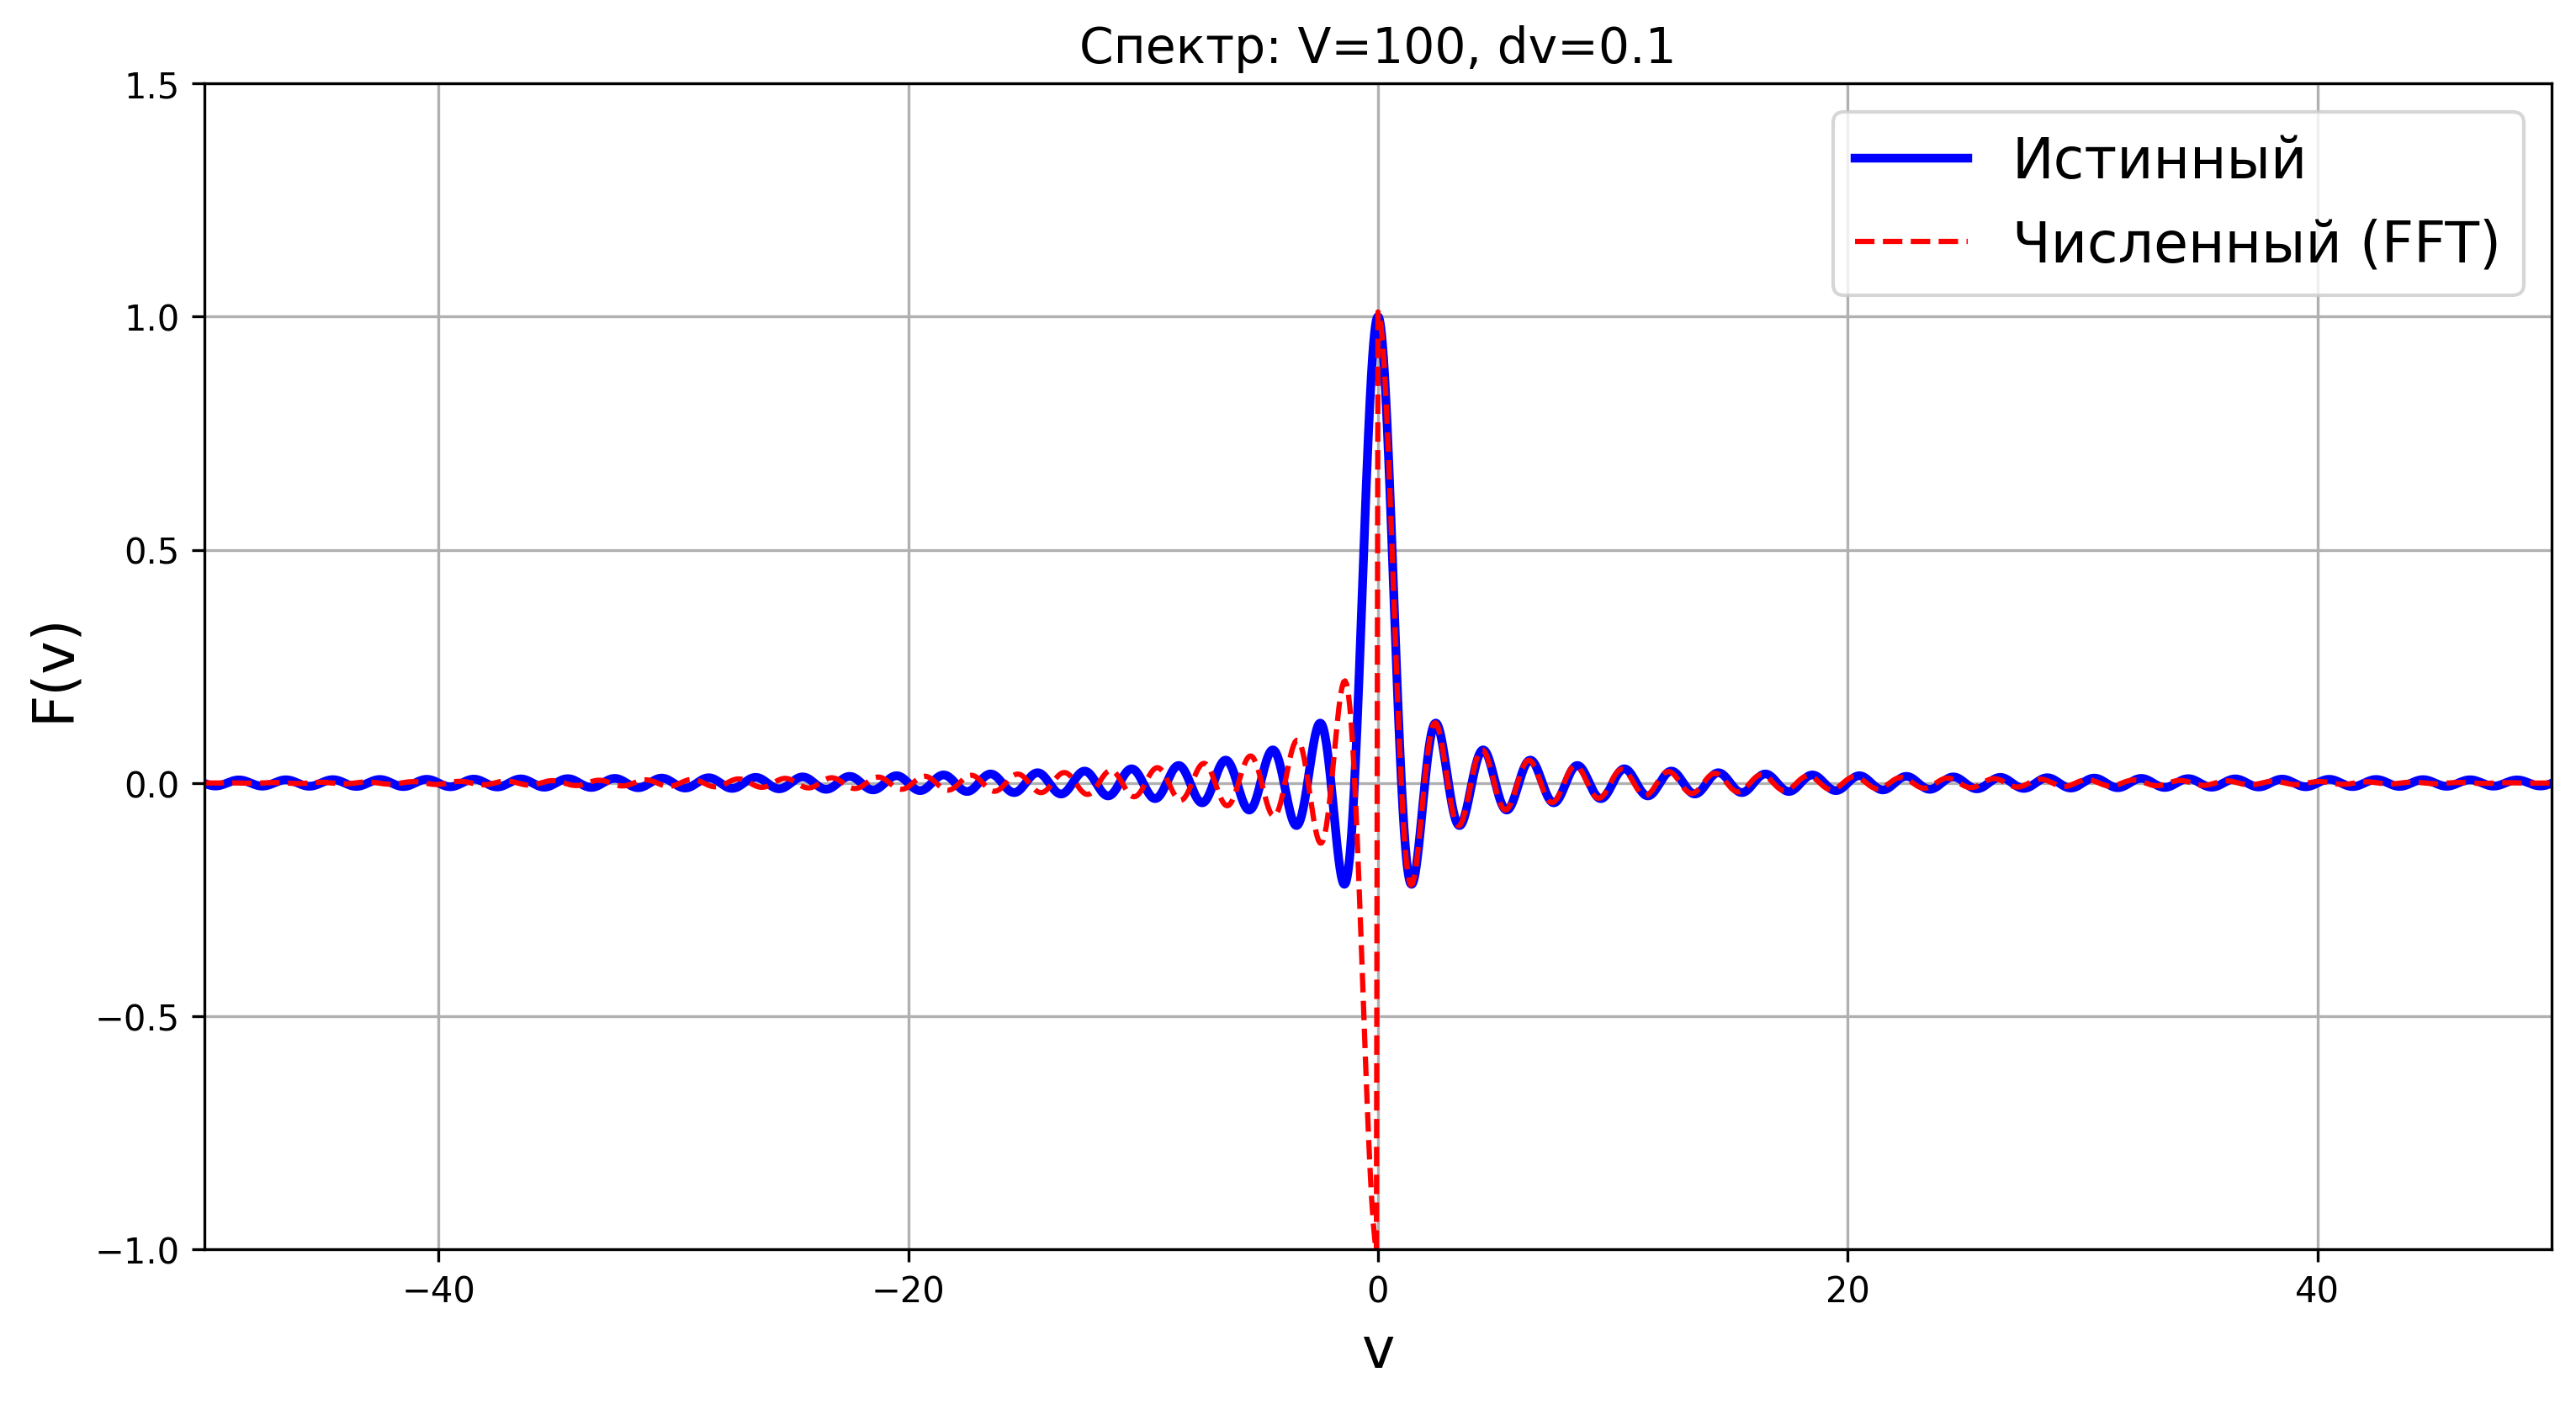
\includegraphics[width=0.95\textwidth]{images/FFTc_T15_V100_dt0.010_dv0.100_spectrum.png}
    \caption{Сравнение спектров: $V=100$, $dv=0.1$.}
\end{figure}

\newpage
\subsection*{Комбинация 3: $T=4$, $V=200$, $dt=0.01$, $dv=0.1$}

\begin{figure}[H]
    \centering
    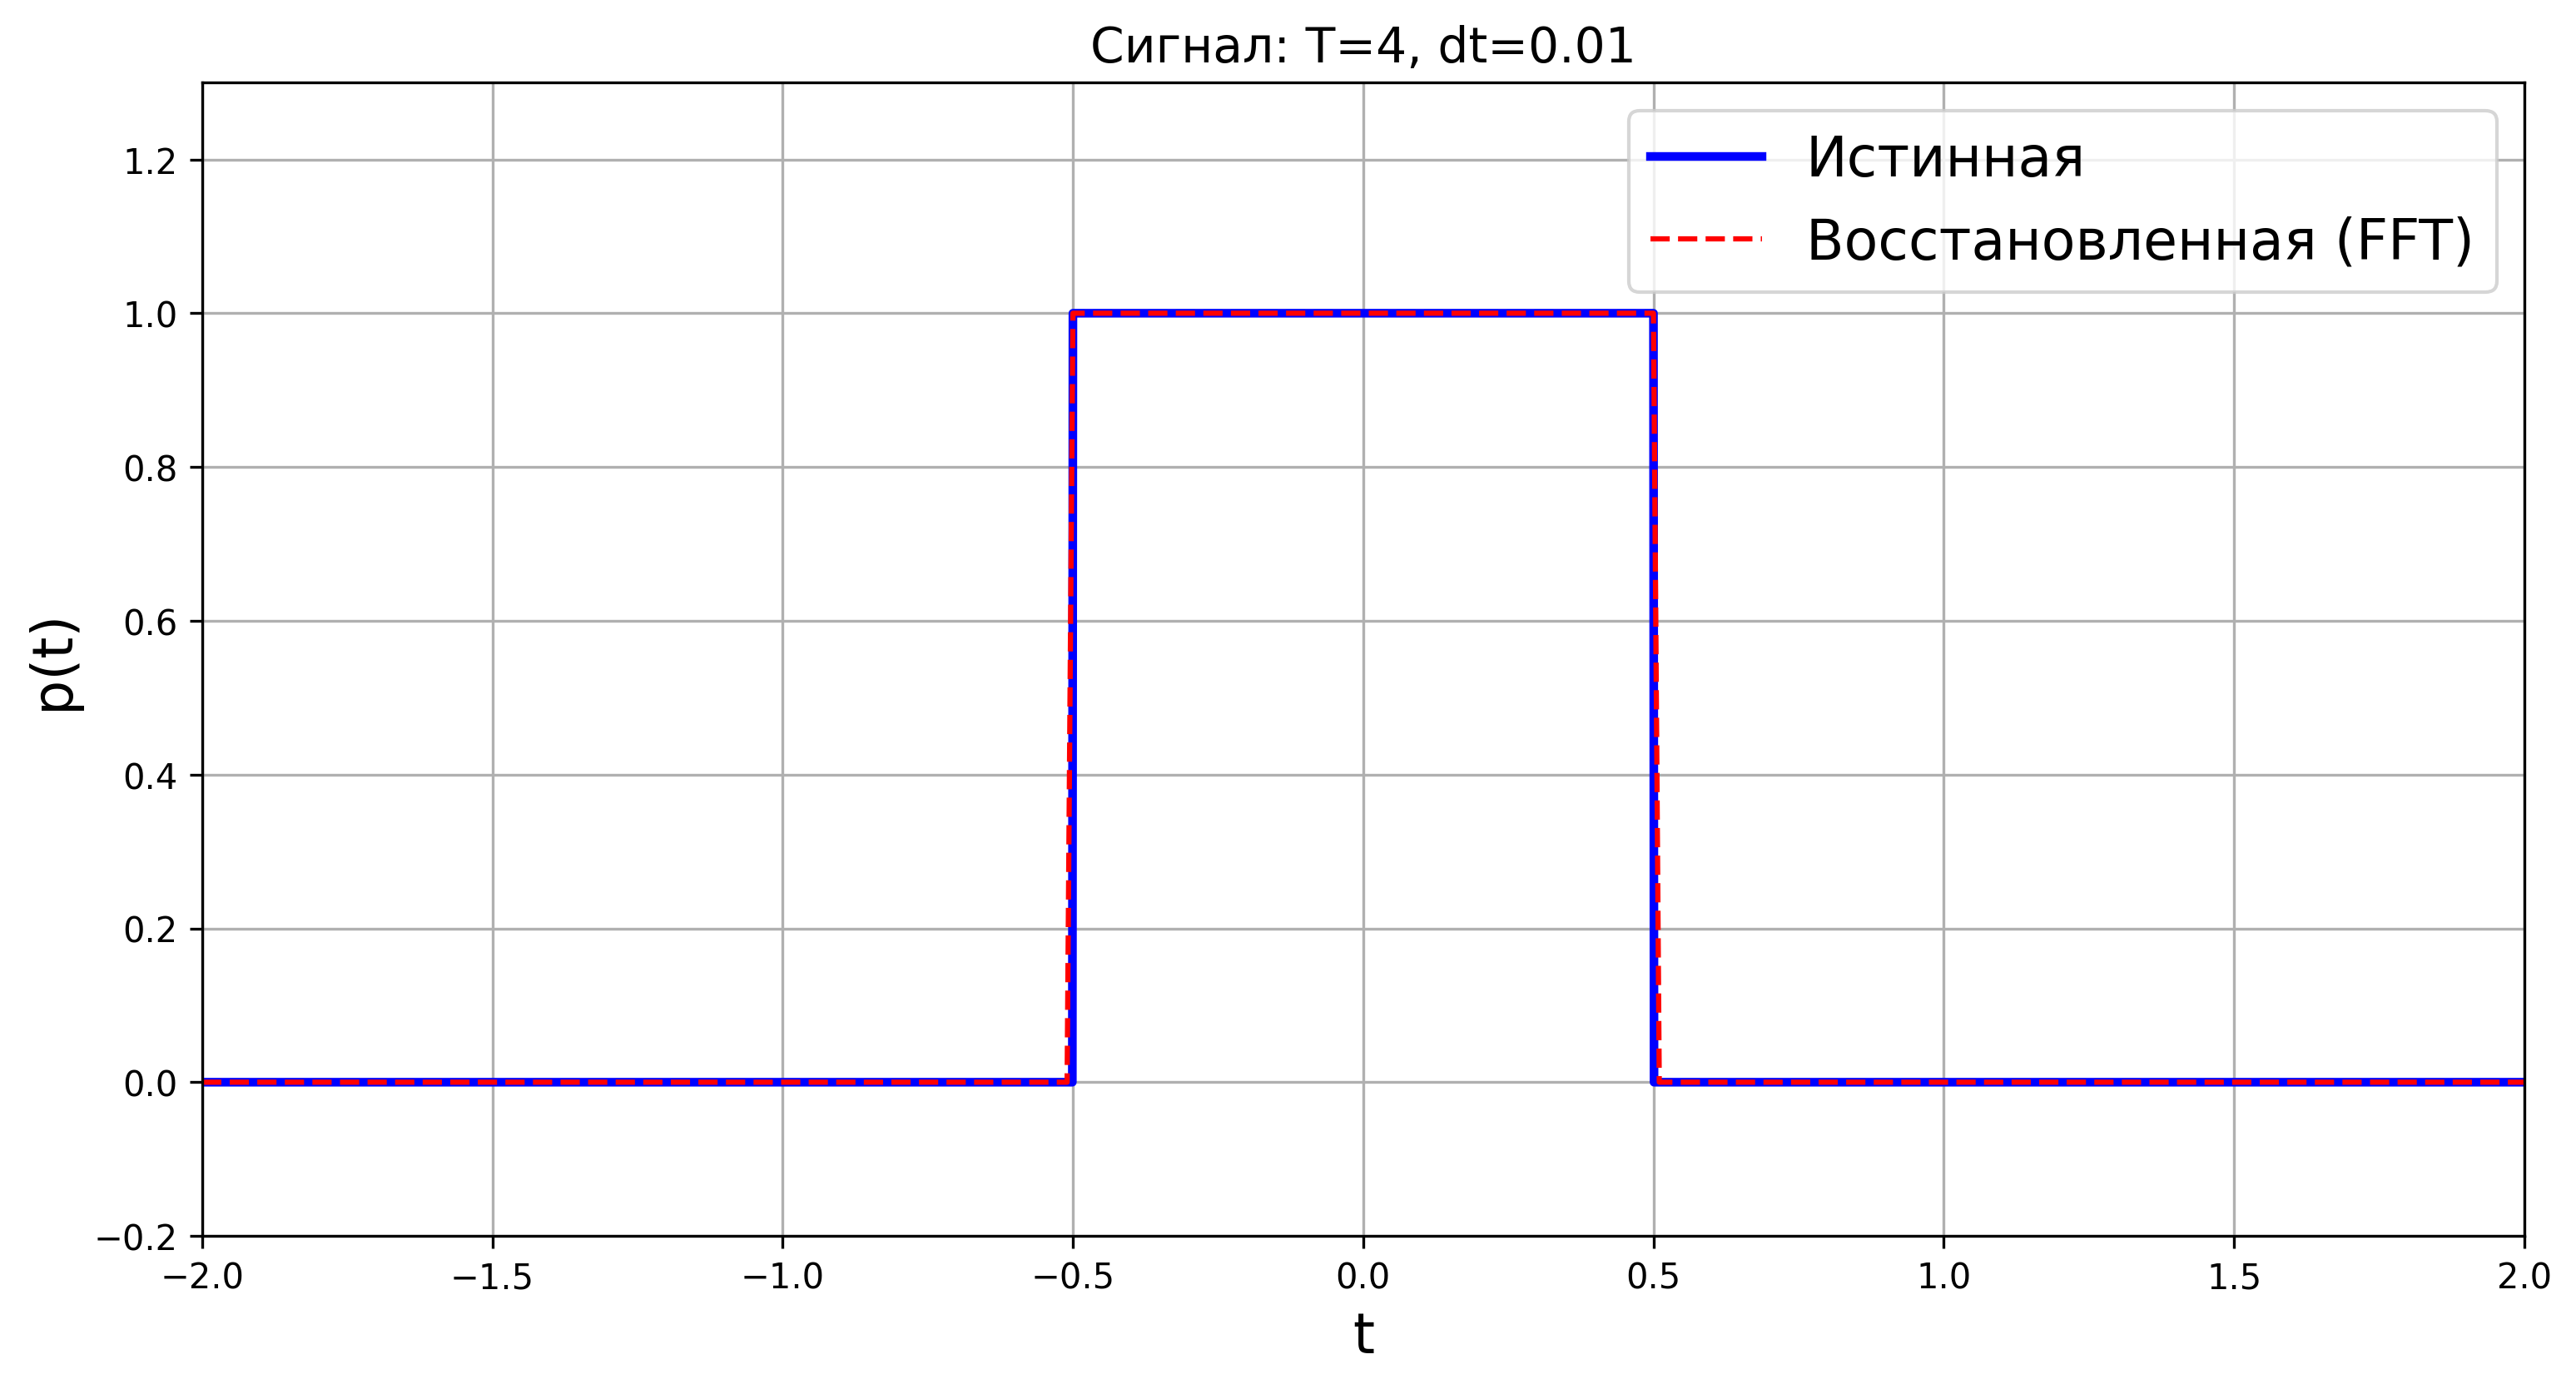
\includegraphics[width=0.95\textwidth]{images/FFTc_T4_V200_dt0.010_dv0.100_signal.png}
    \caption{Восстановление сигнала: $T=4$, $dt=0.01$.}
\end{figure}

\begin{figure}[H]
    \centering
    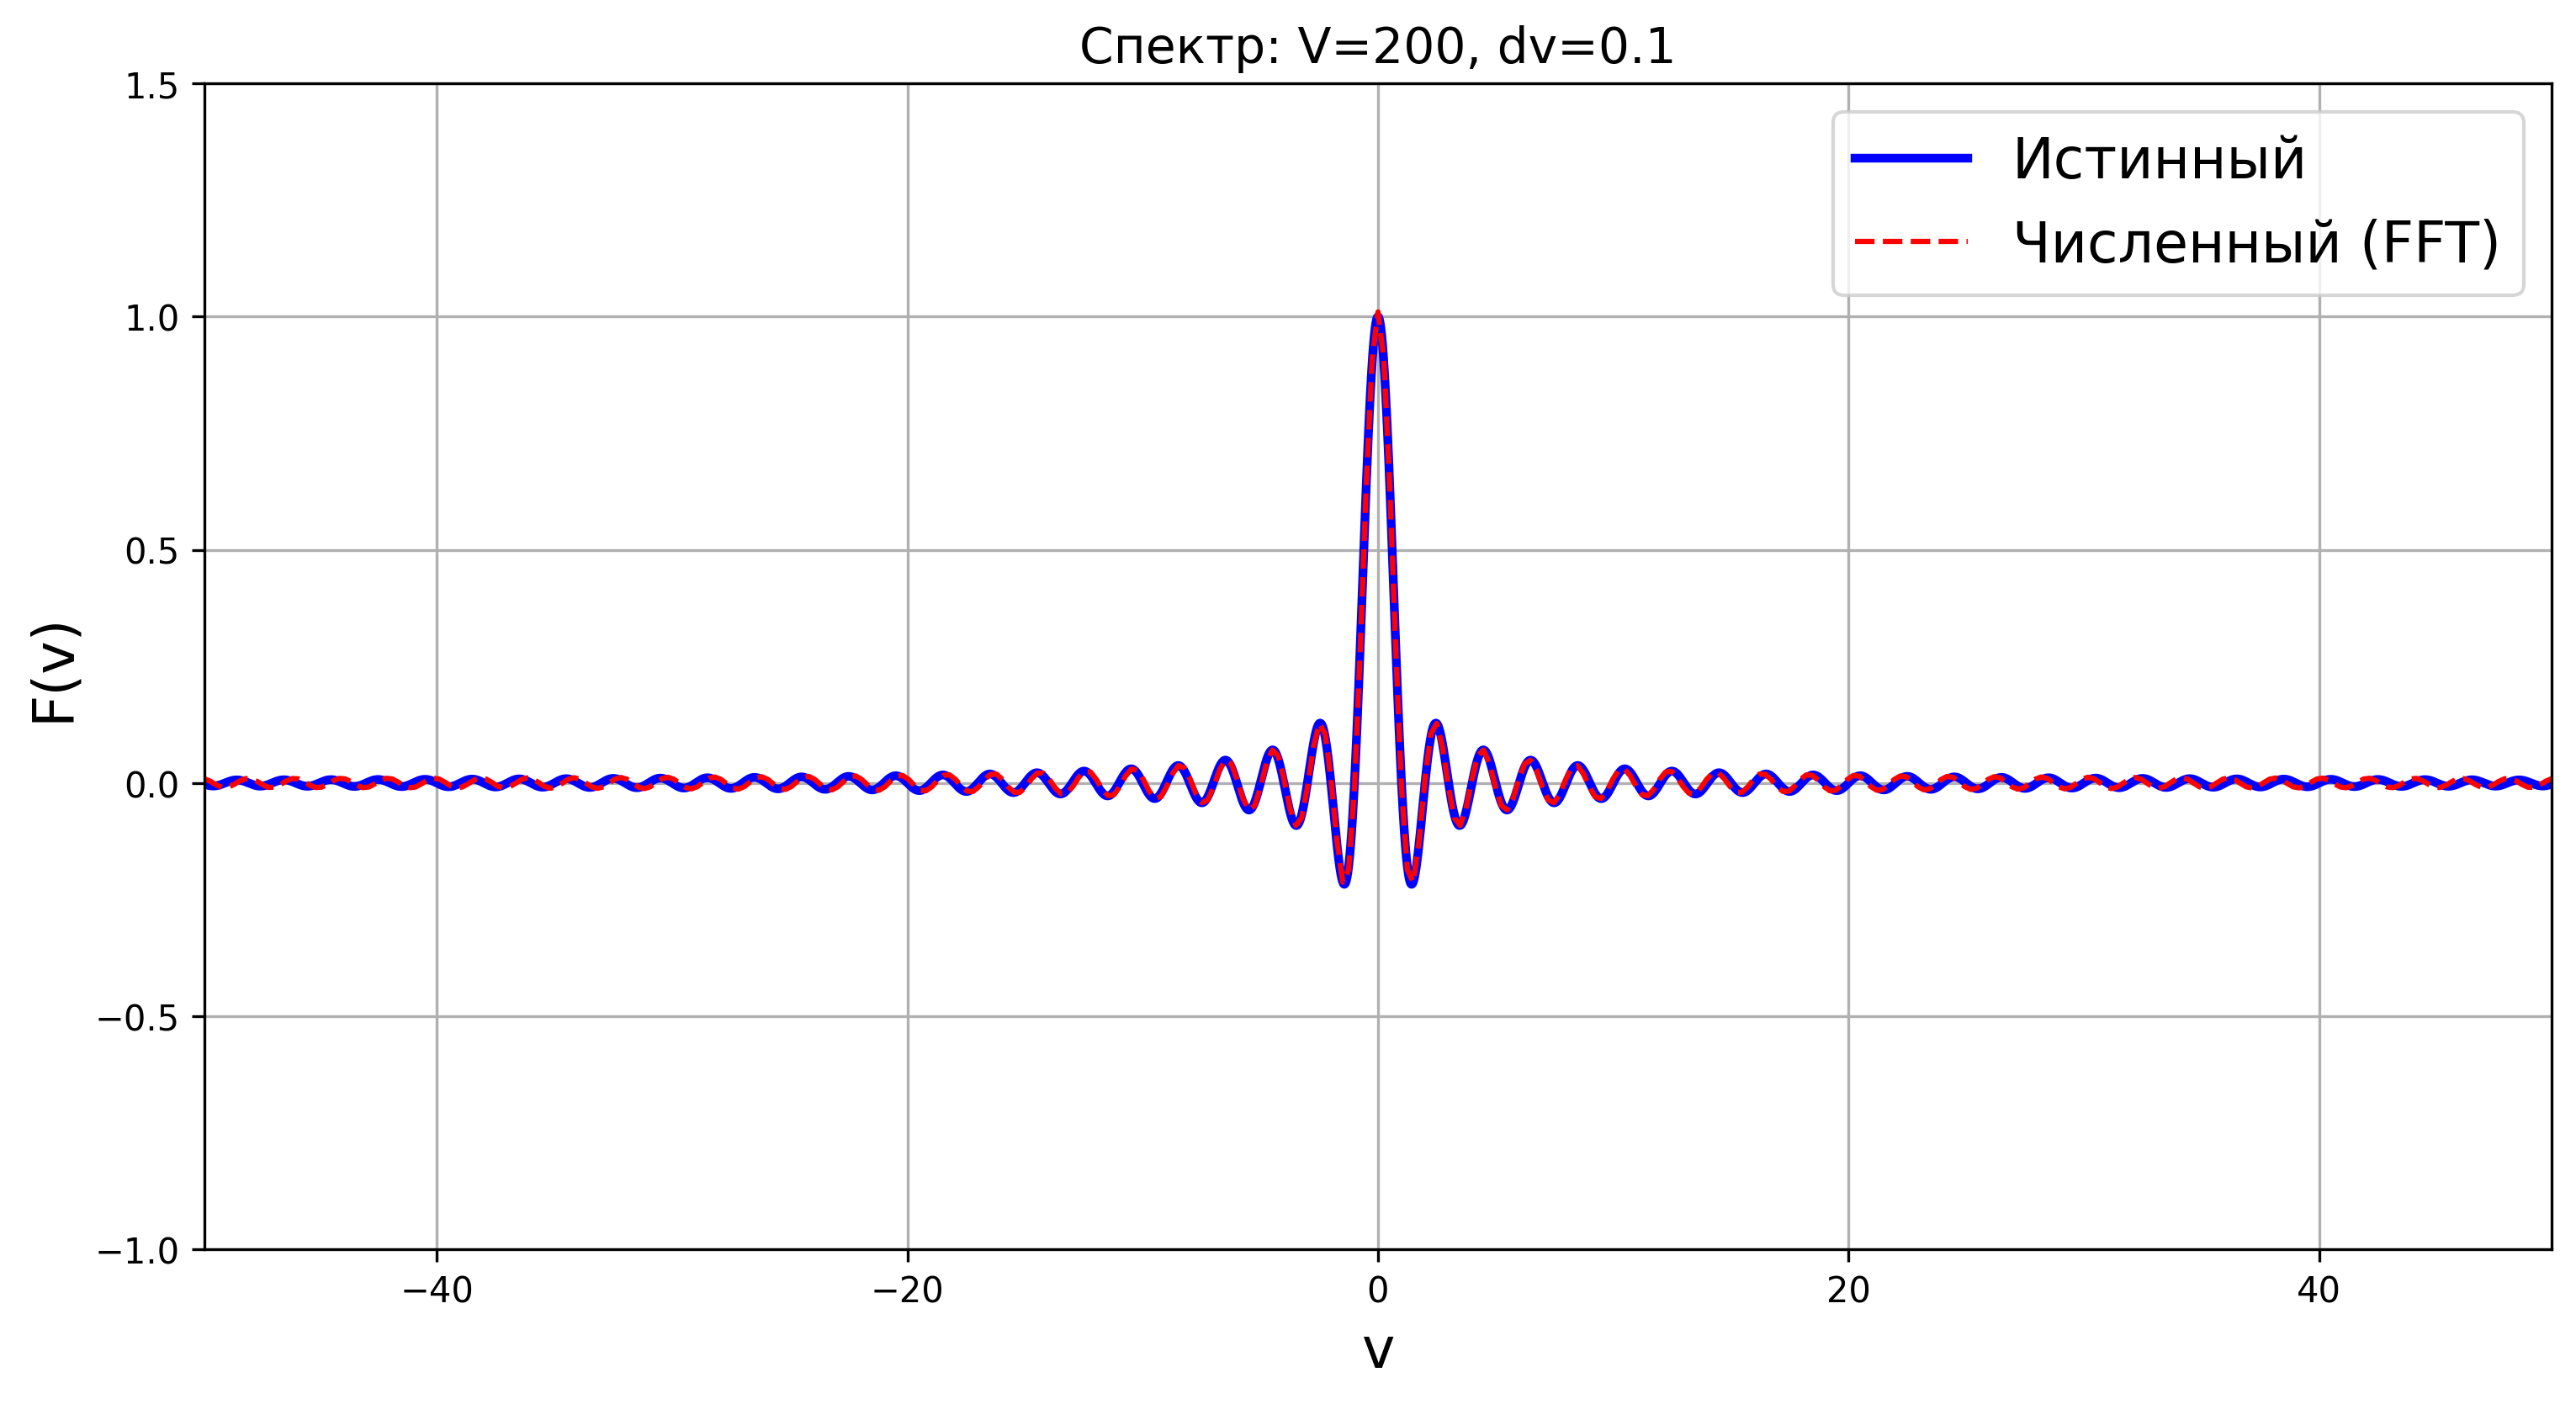
\includegraphics[width=0.95\textwidth]{images/FFTc_T4_V200_dt0.010_dv0.100_spectrum.png}
    \caption{Сравнение спектров: $V=200$, $dv=0.1$.}
\end{figure}

\newpage
\subsection*{Комбинация 4: $T=4$, $V=100$, $dt=0.1$, $dv=0.1$}

\begin{figure}[H]
    \centering
    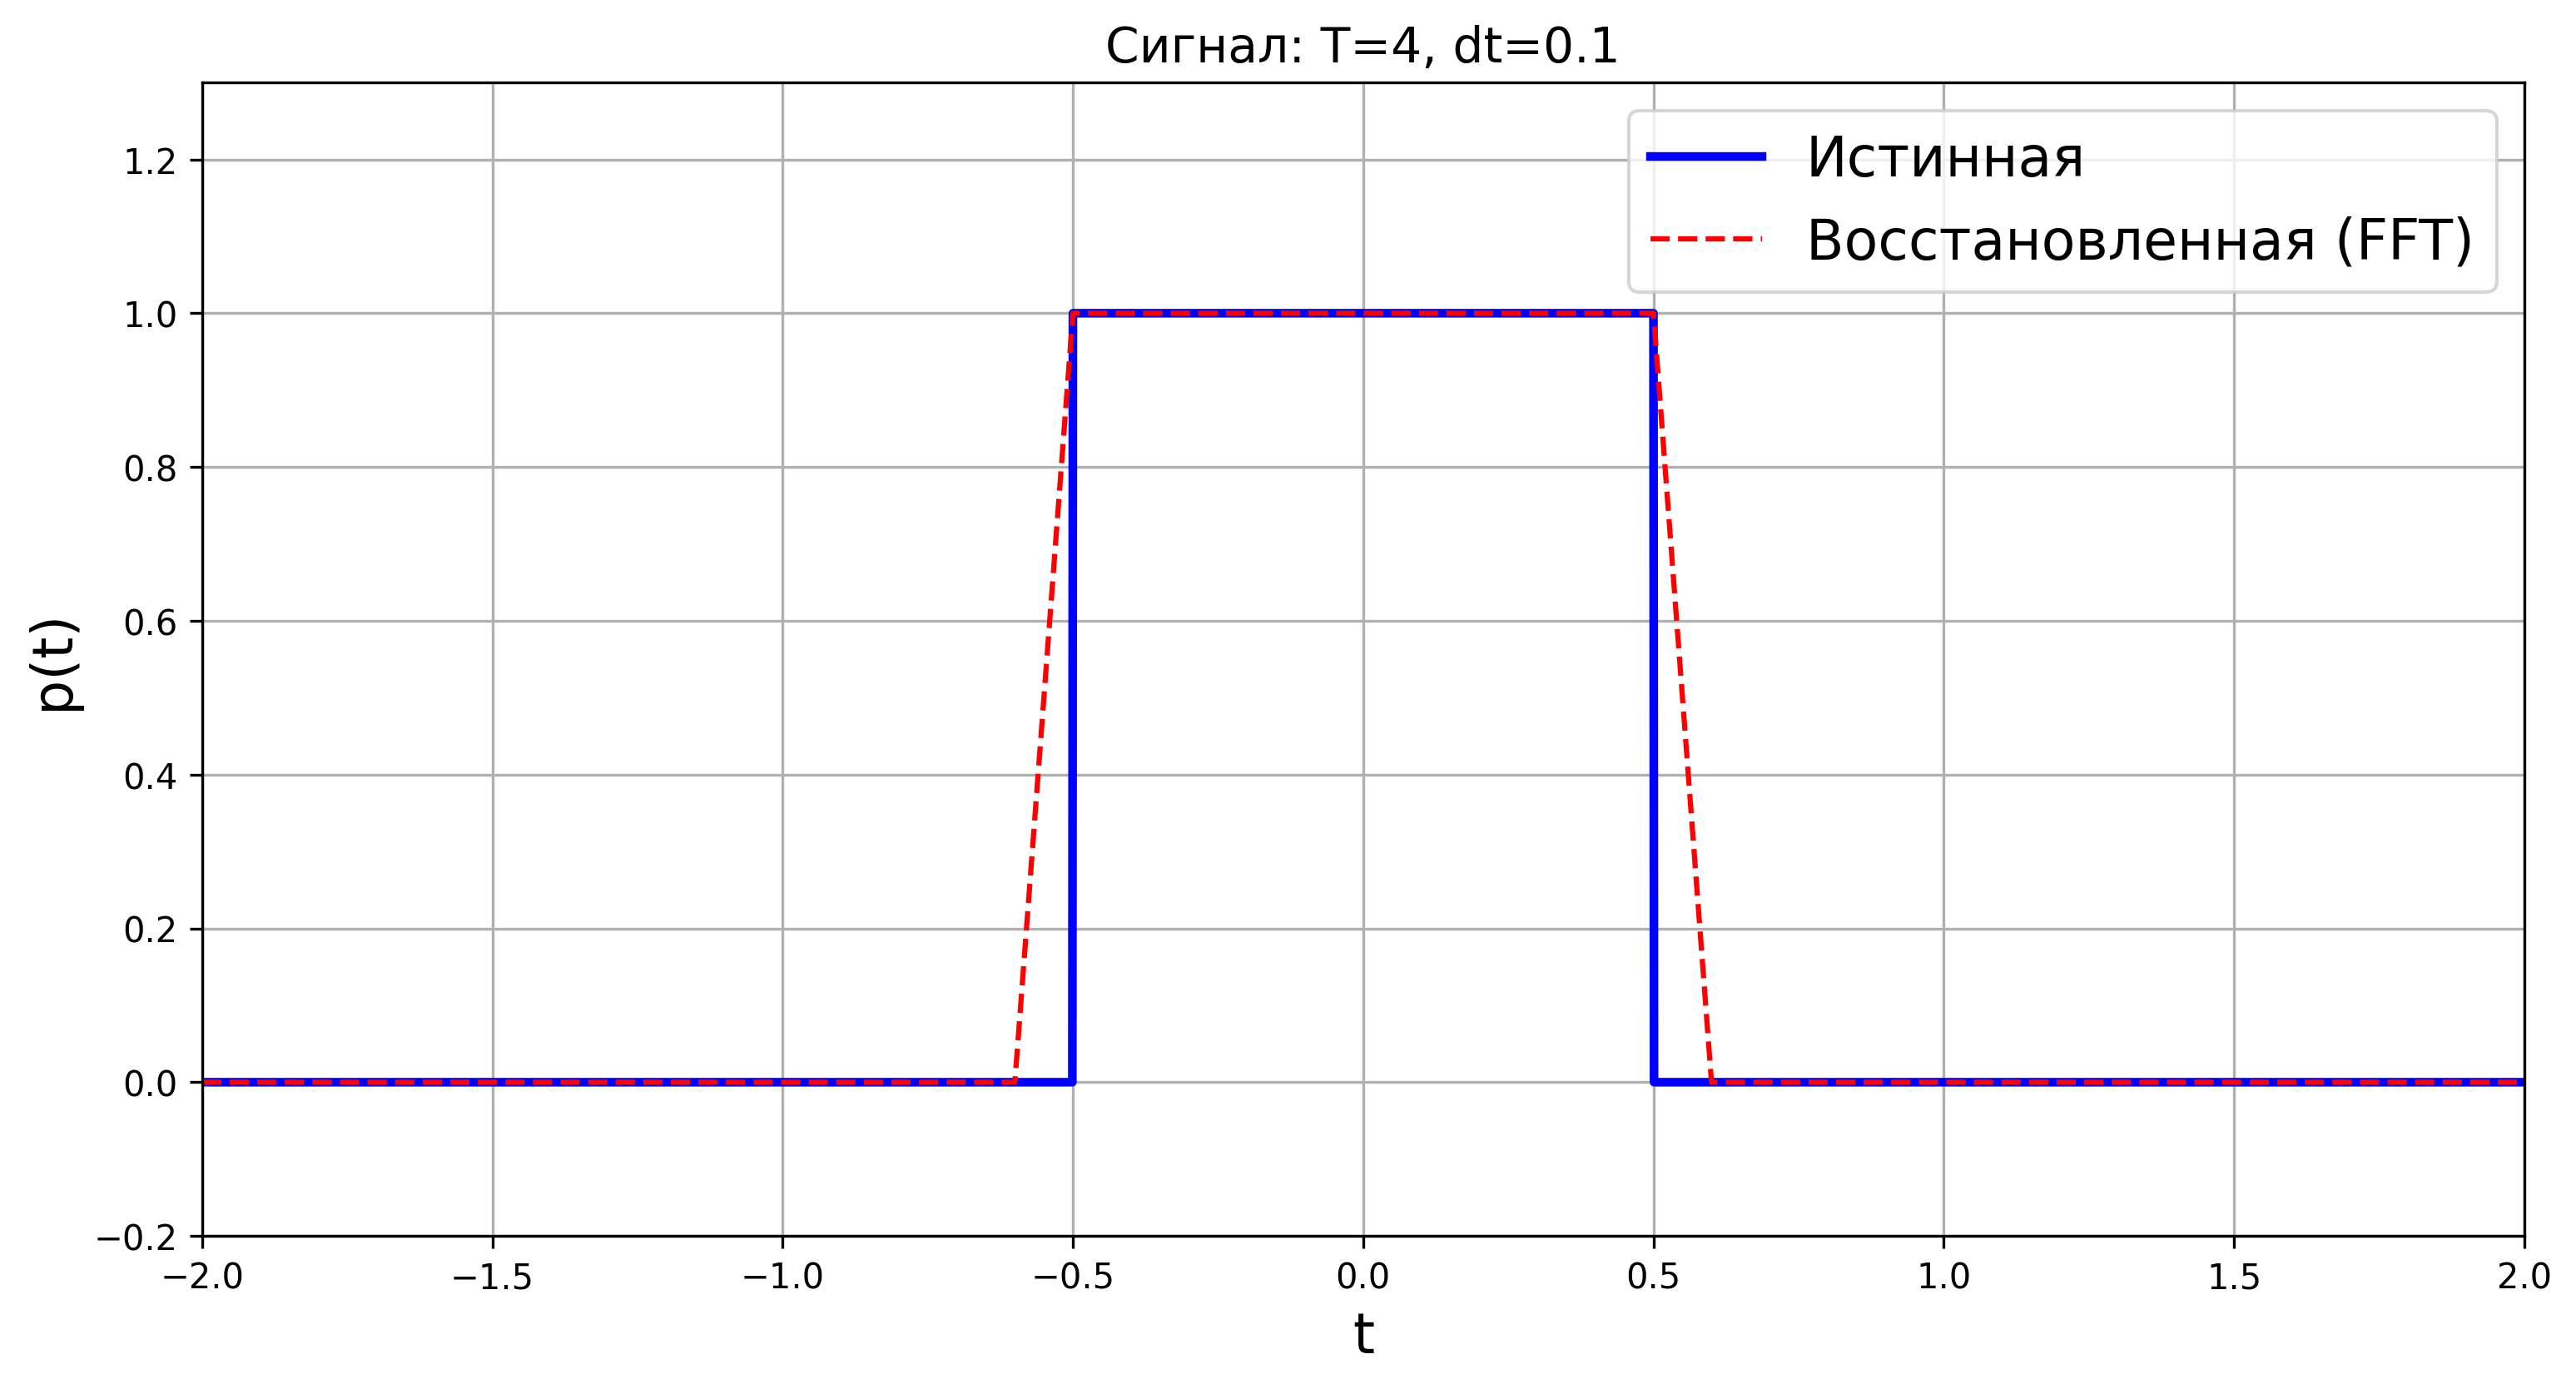
\includegraphics[width=0.95\textwidth]{images/FFTc_T4_V100_dt0.100_dv0.100_signal.png}
    \caption{Восстановление сигнала: $T=4$, $dt=0.1$.}
\end{figure}

\begin{figure}[H]
    \centering
    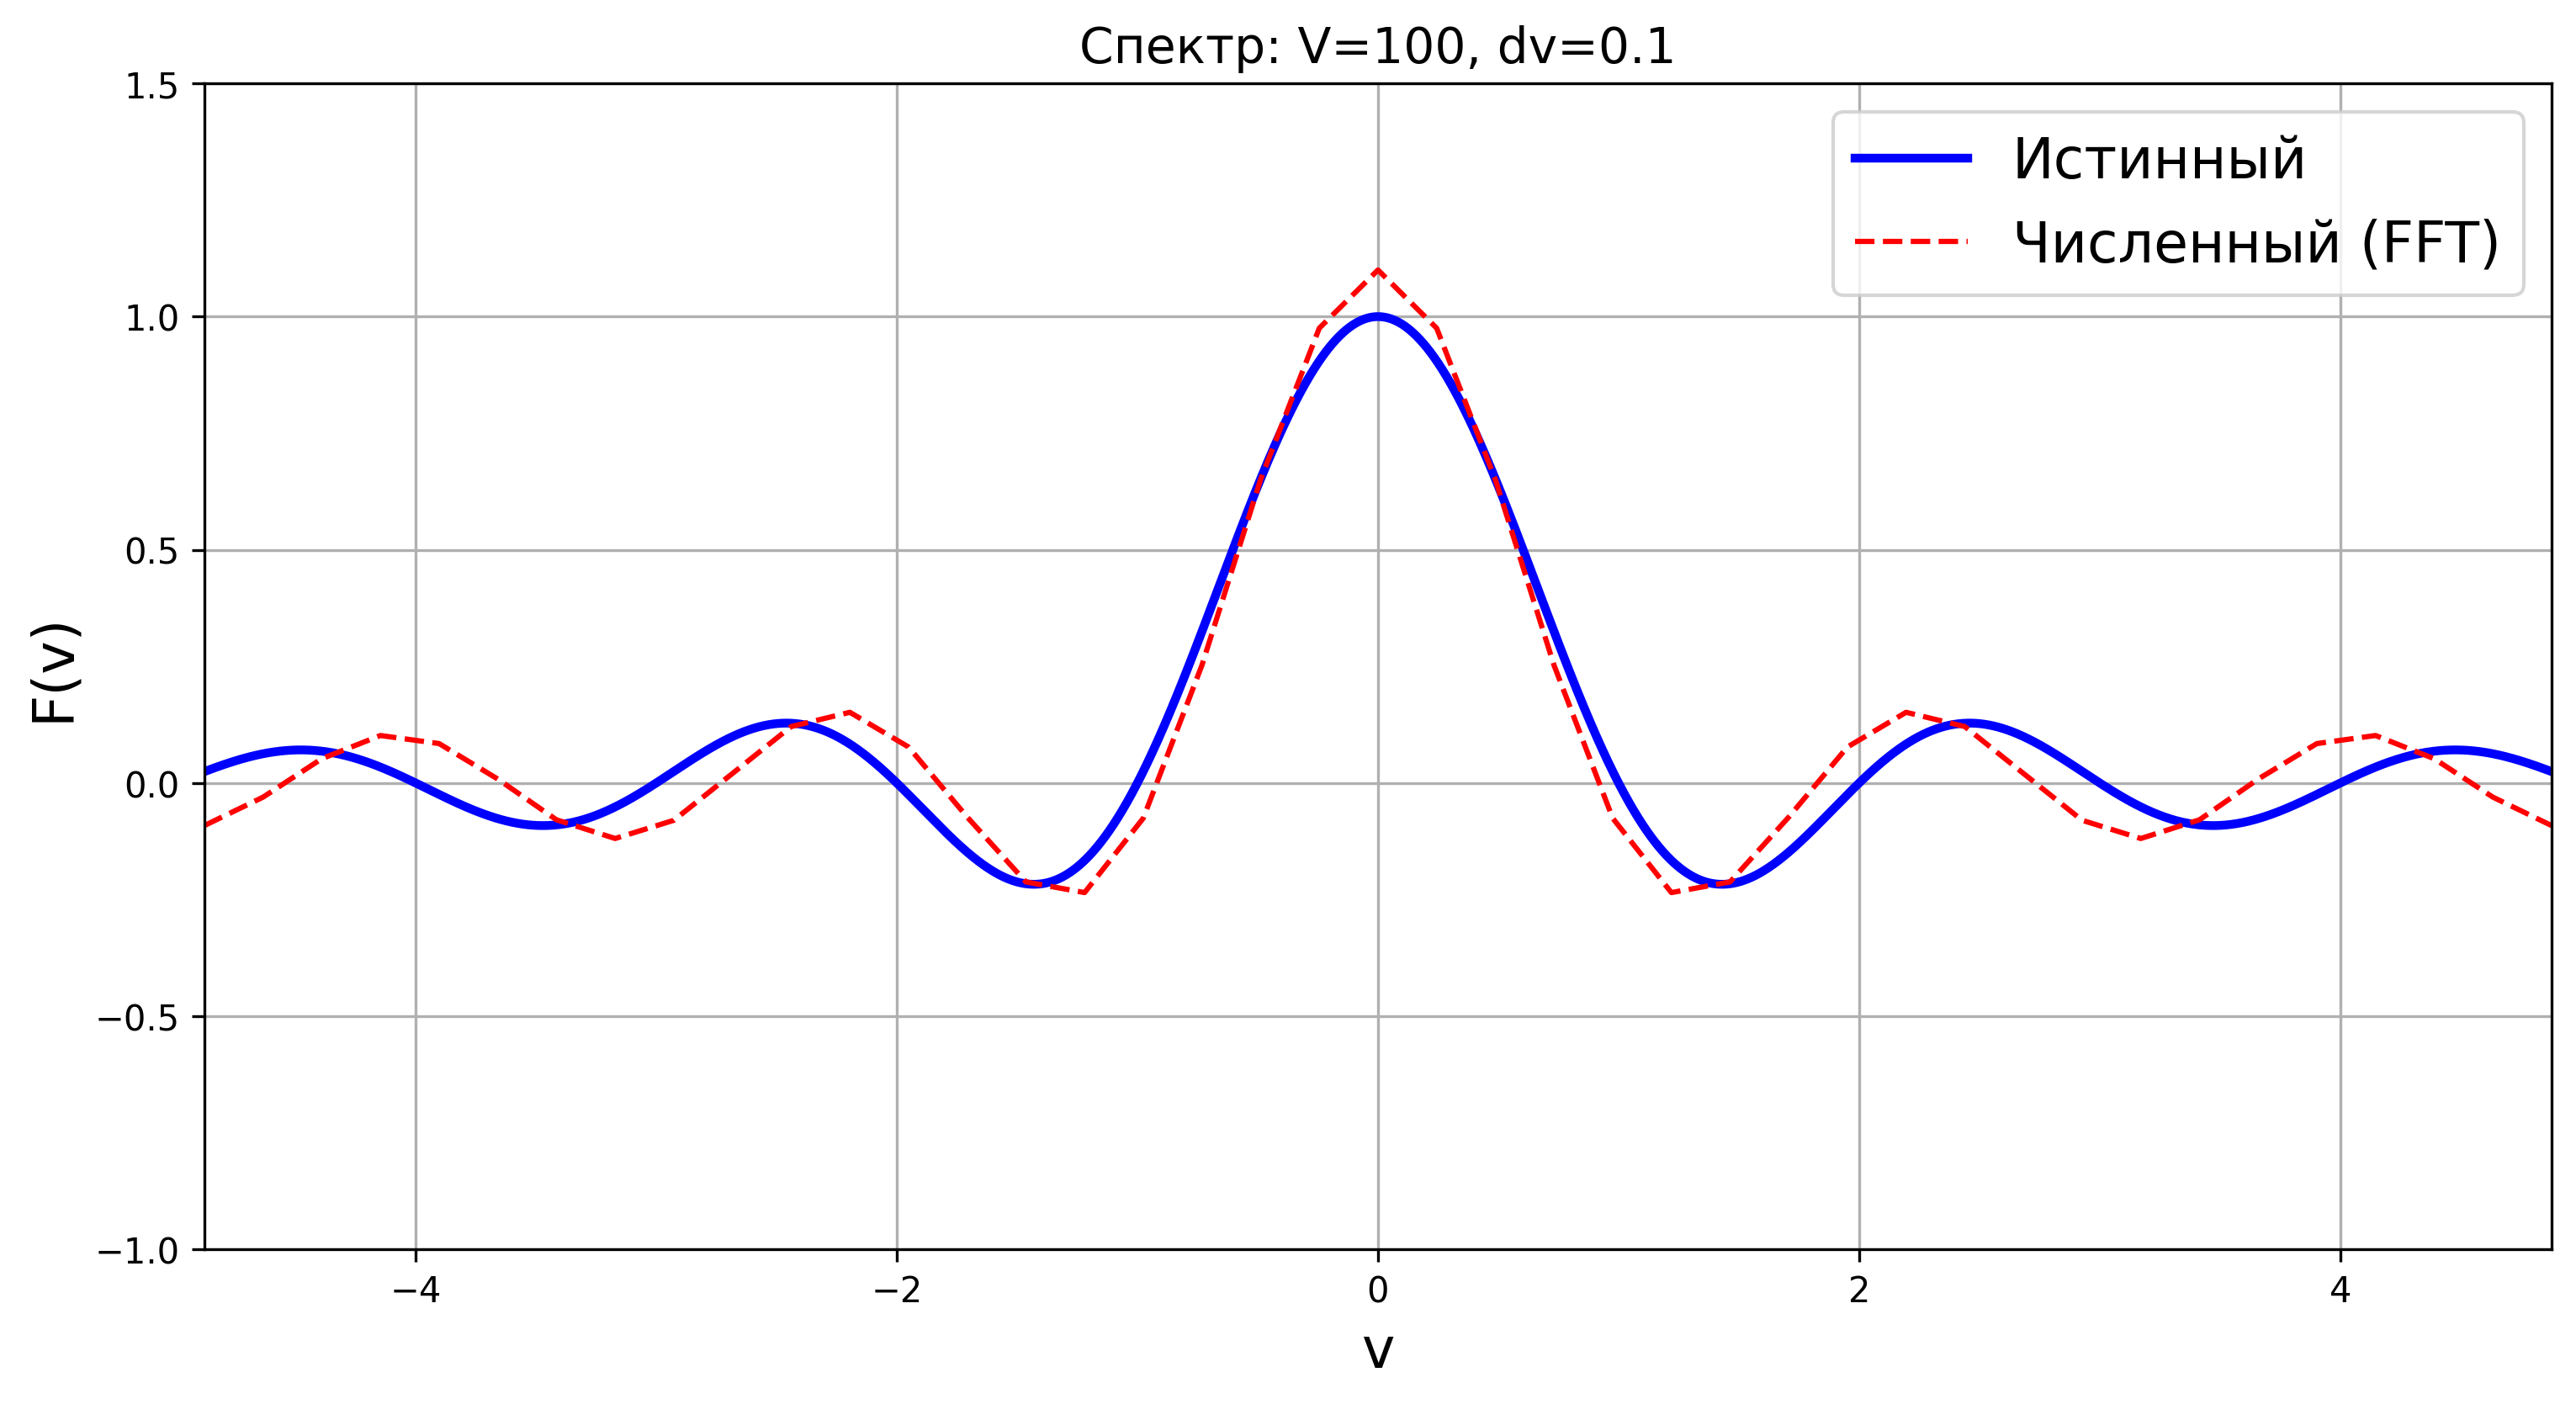
\includegraphics[width=0.95\textwidth]{images/FFTc_T4_V100_dt0.100_dv0.100_spectrum.png}
    \caption{Сравнение спектров: $V=100$, $dv=0.1$.}
\end{figure}

\newpage
\subsection*{Комбинация 5: $T=4$, $V=100$, $dt=0.01$, $dv=0.5$}

\begin{figure}[H]
    \centering
    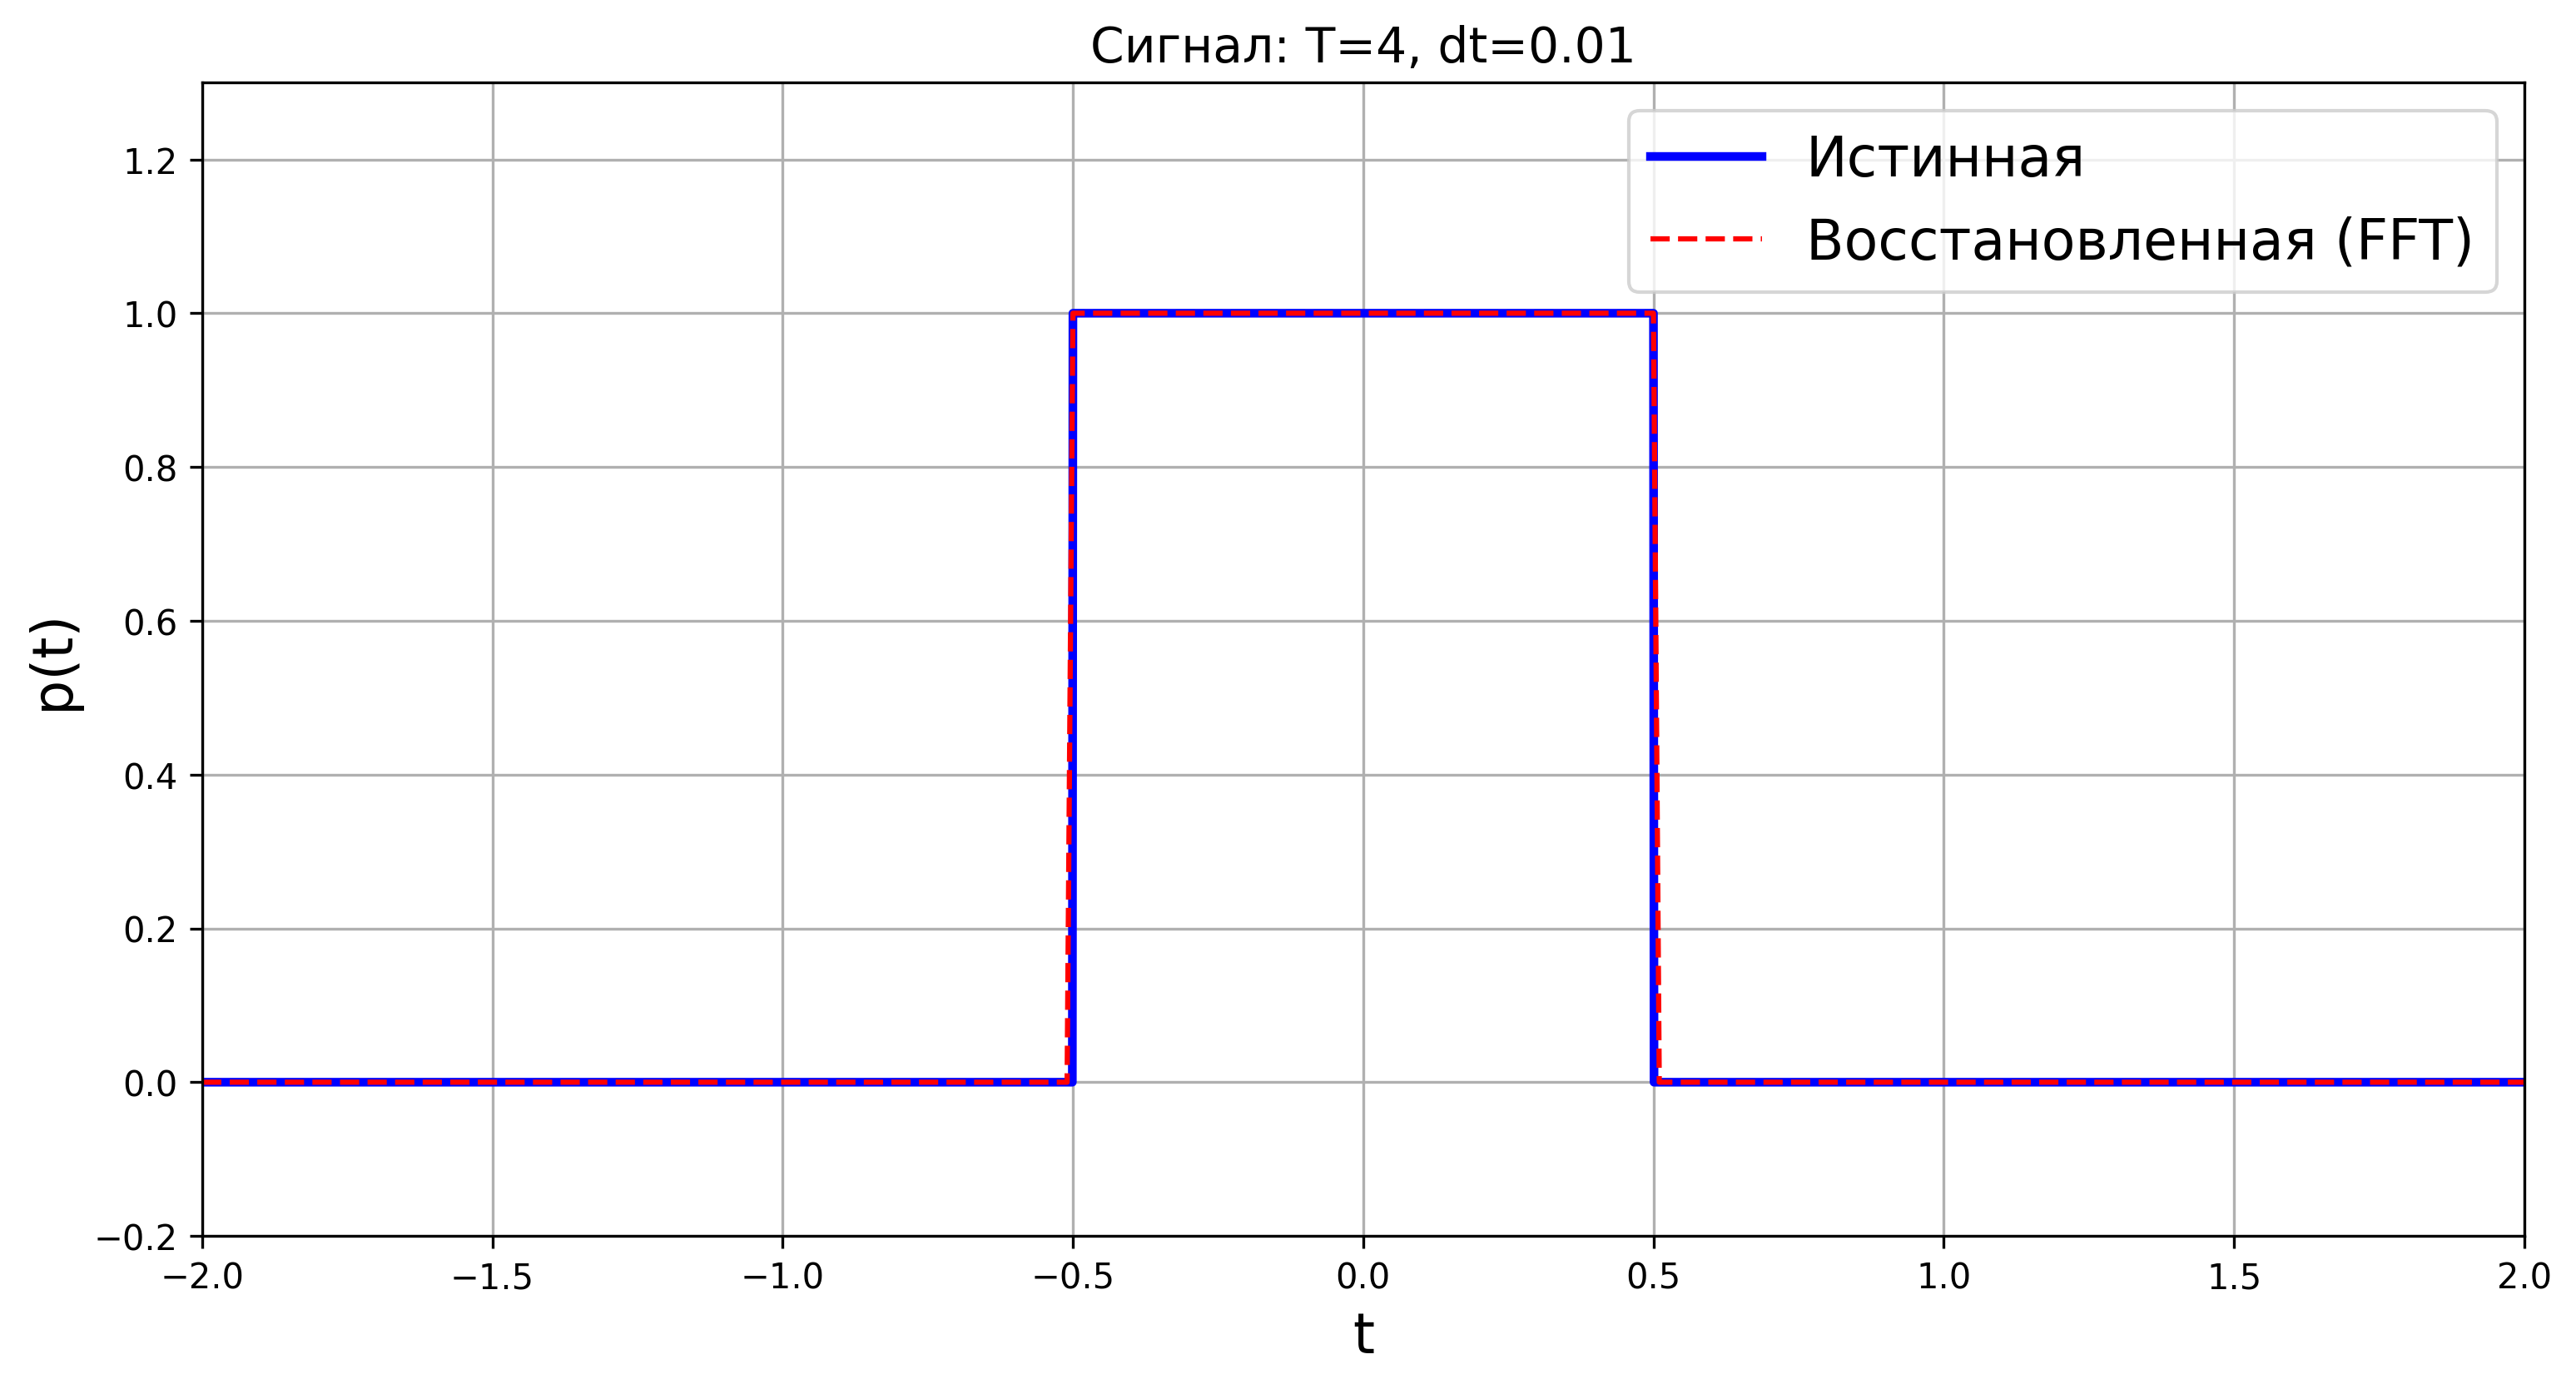
\includegraphics[width=0.95\textwidth]{images/FFTc_T4_V100_dt0.010_dv0.500_signal.png}
    \caption{Восстановление сигнала: $T=4$, $dt=0.01$.}
\end{figure}

\begin{figure}[H]
    \centering
    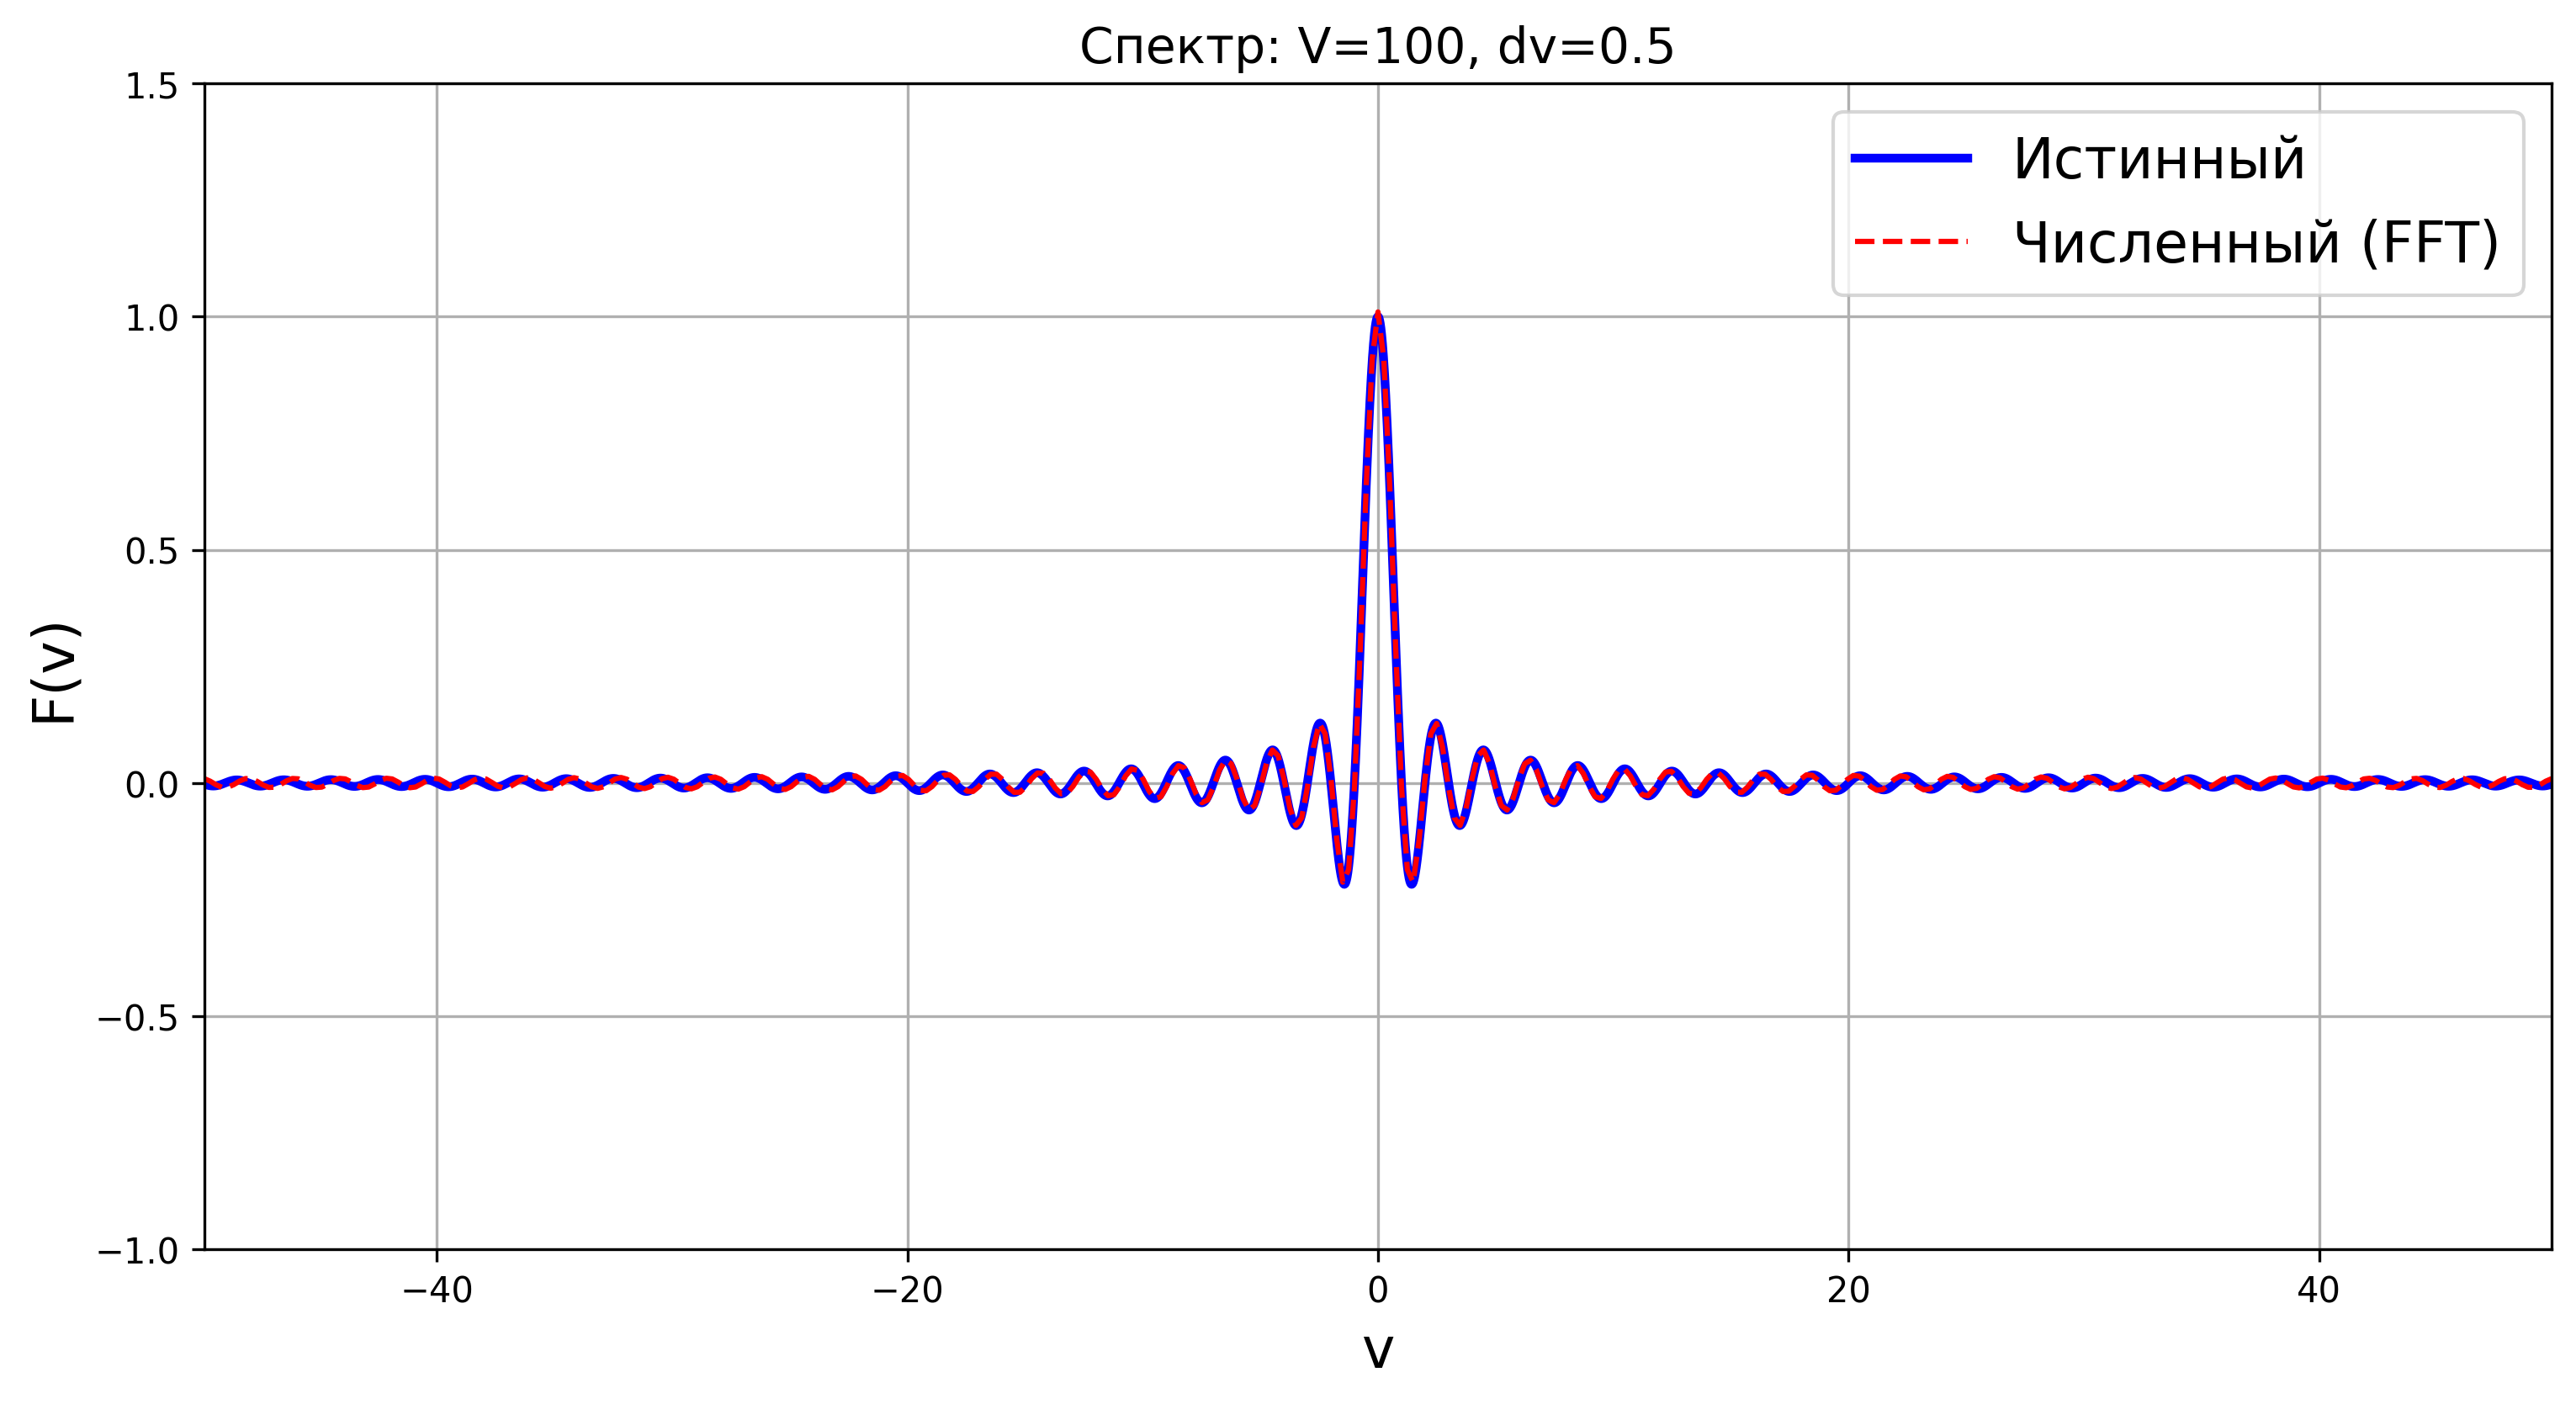
\includegraphics[width=0.95\textwidth]{images/FFTc_T4_V100_dt0.010_dv0.500_spectrum.png}
    \caption{Сравнение спектров: $V=100$, $dv=0.5$.}
\end{figure}



Как видно из графиков, теперь фурье образы максимально близки к истинным. 
\newpage
\subsection{Сравнение всех методов}
\subsection*{Комбинация 1: $T=4$, $V=100$, $dt=0.01$, $dv=0.1$}

\begin{figure}[H]
    \centering
    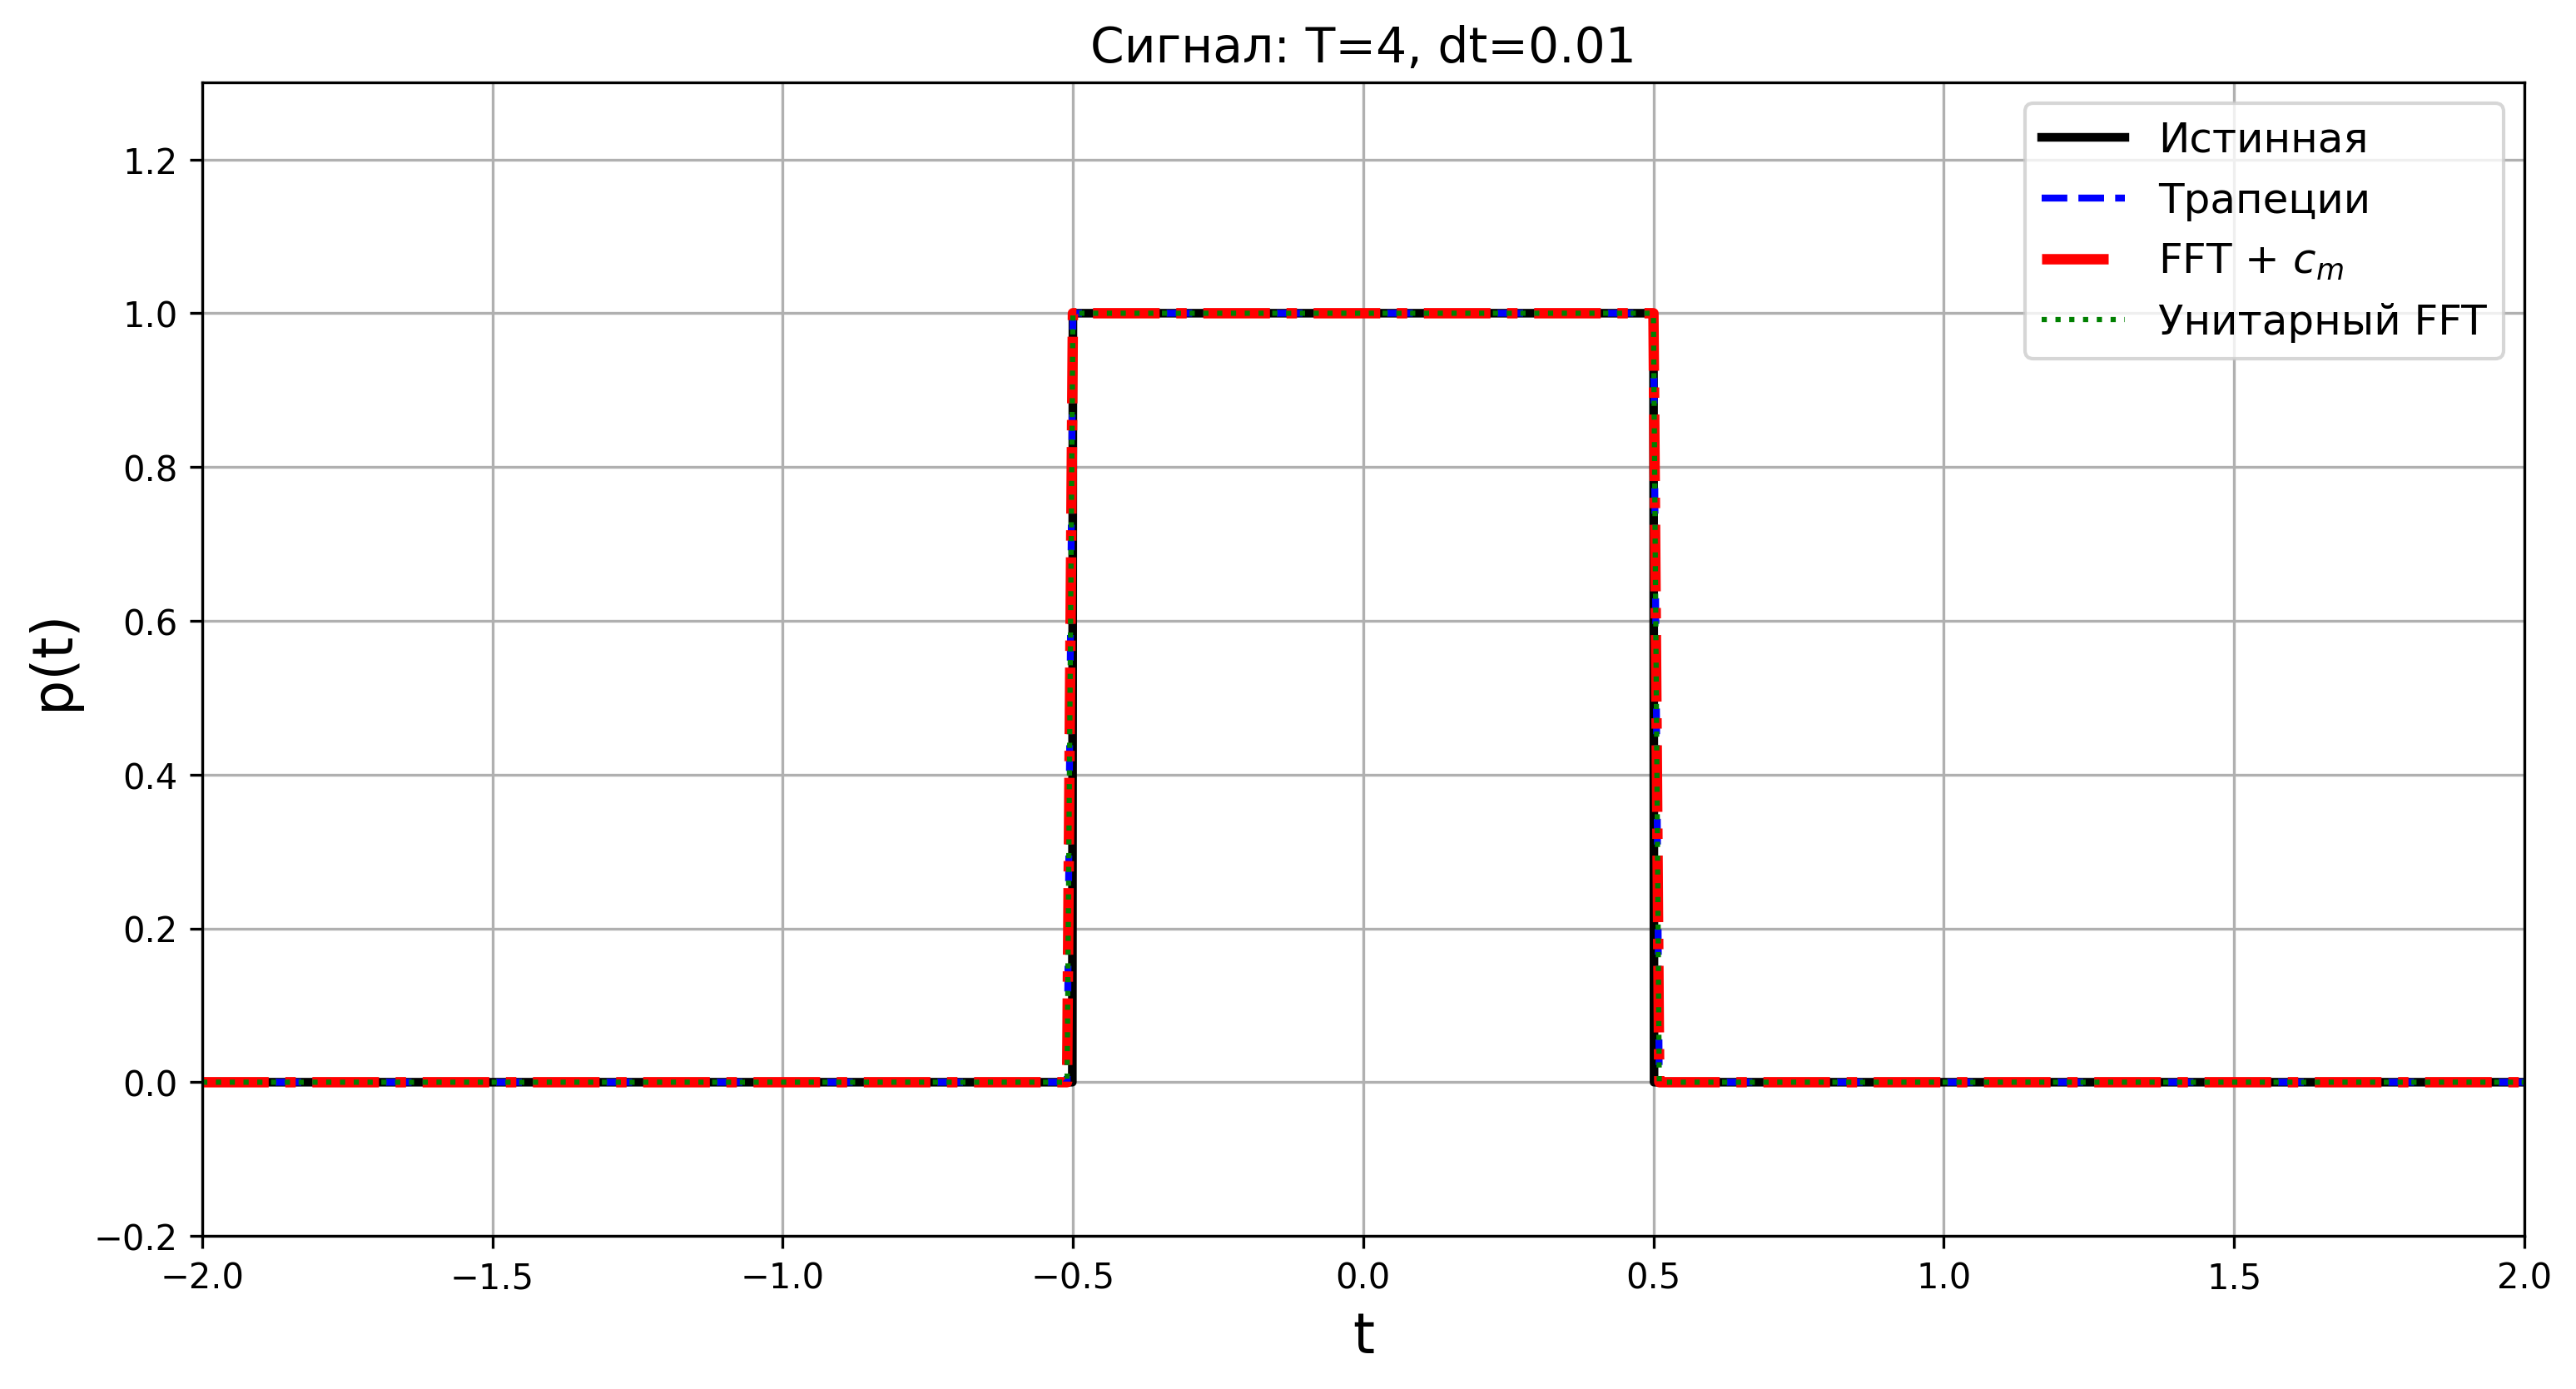
\includegraphics[width=0.95\textwidth]{images/ALL_T4_V100_dt0.010_dv0.100_signal.png}
    \caption{Восстановление сигнала: $T=4$, $dt=0.01$.}
\end{figure}

\begin{figure}[H]
    \centering
    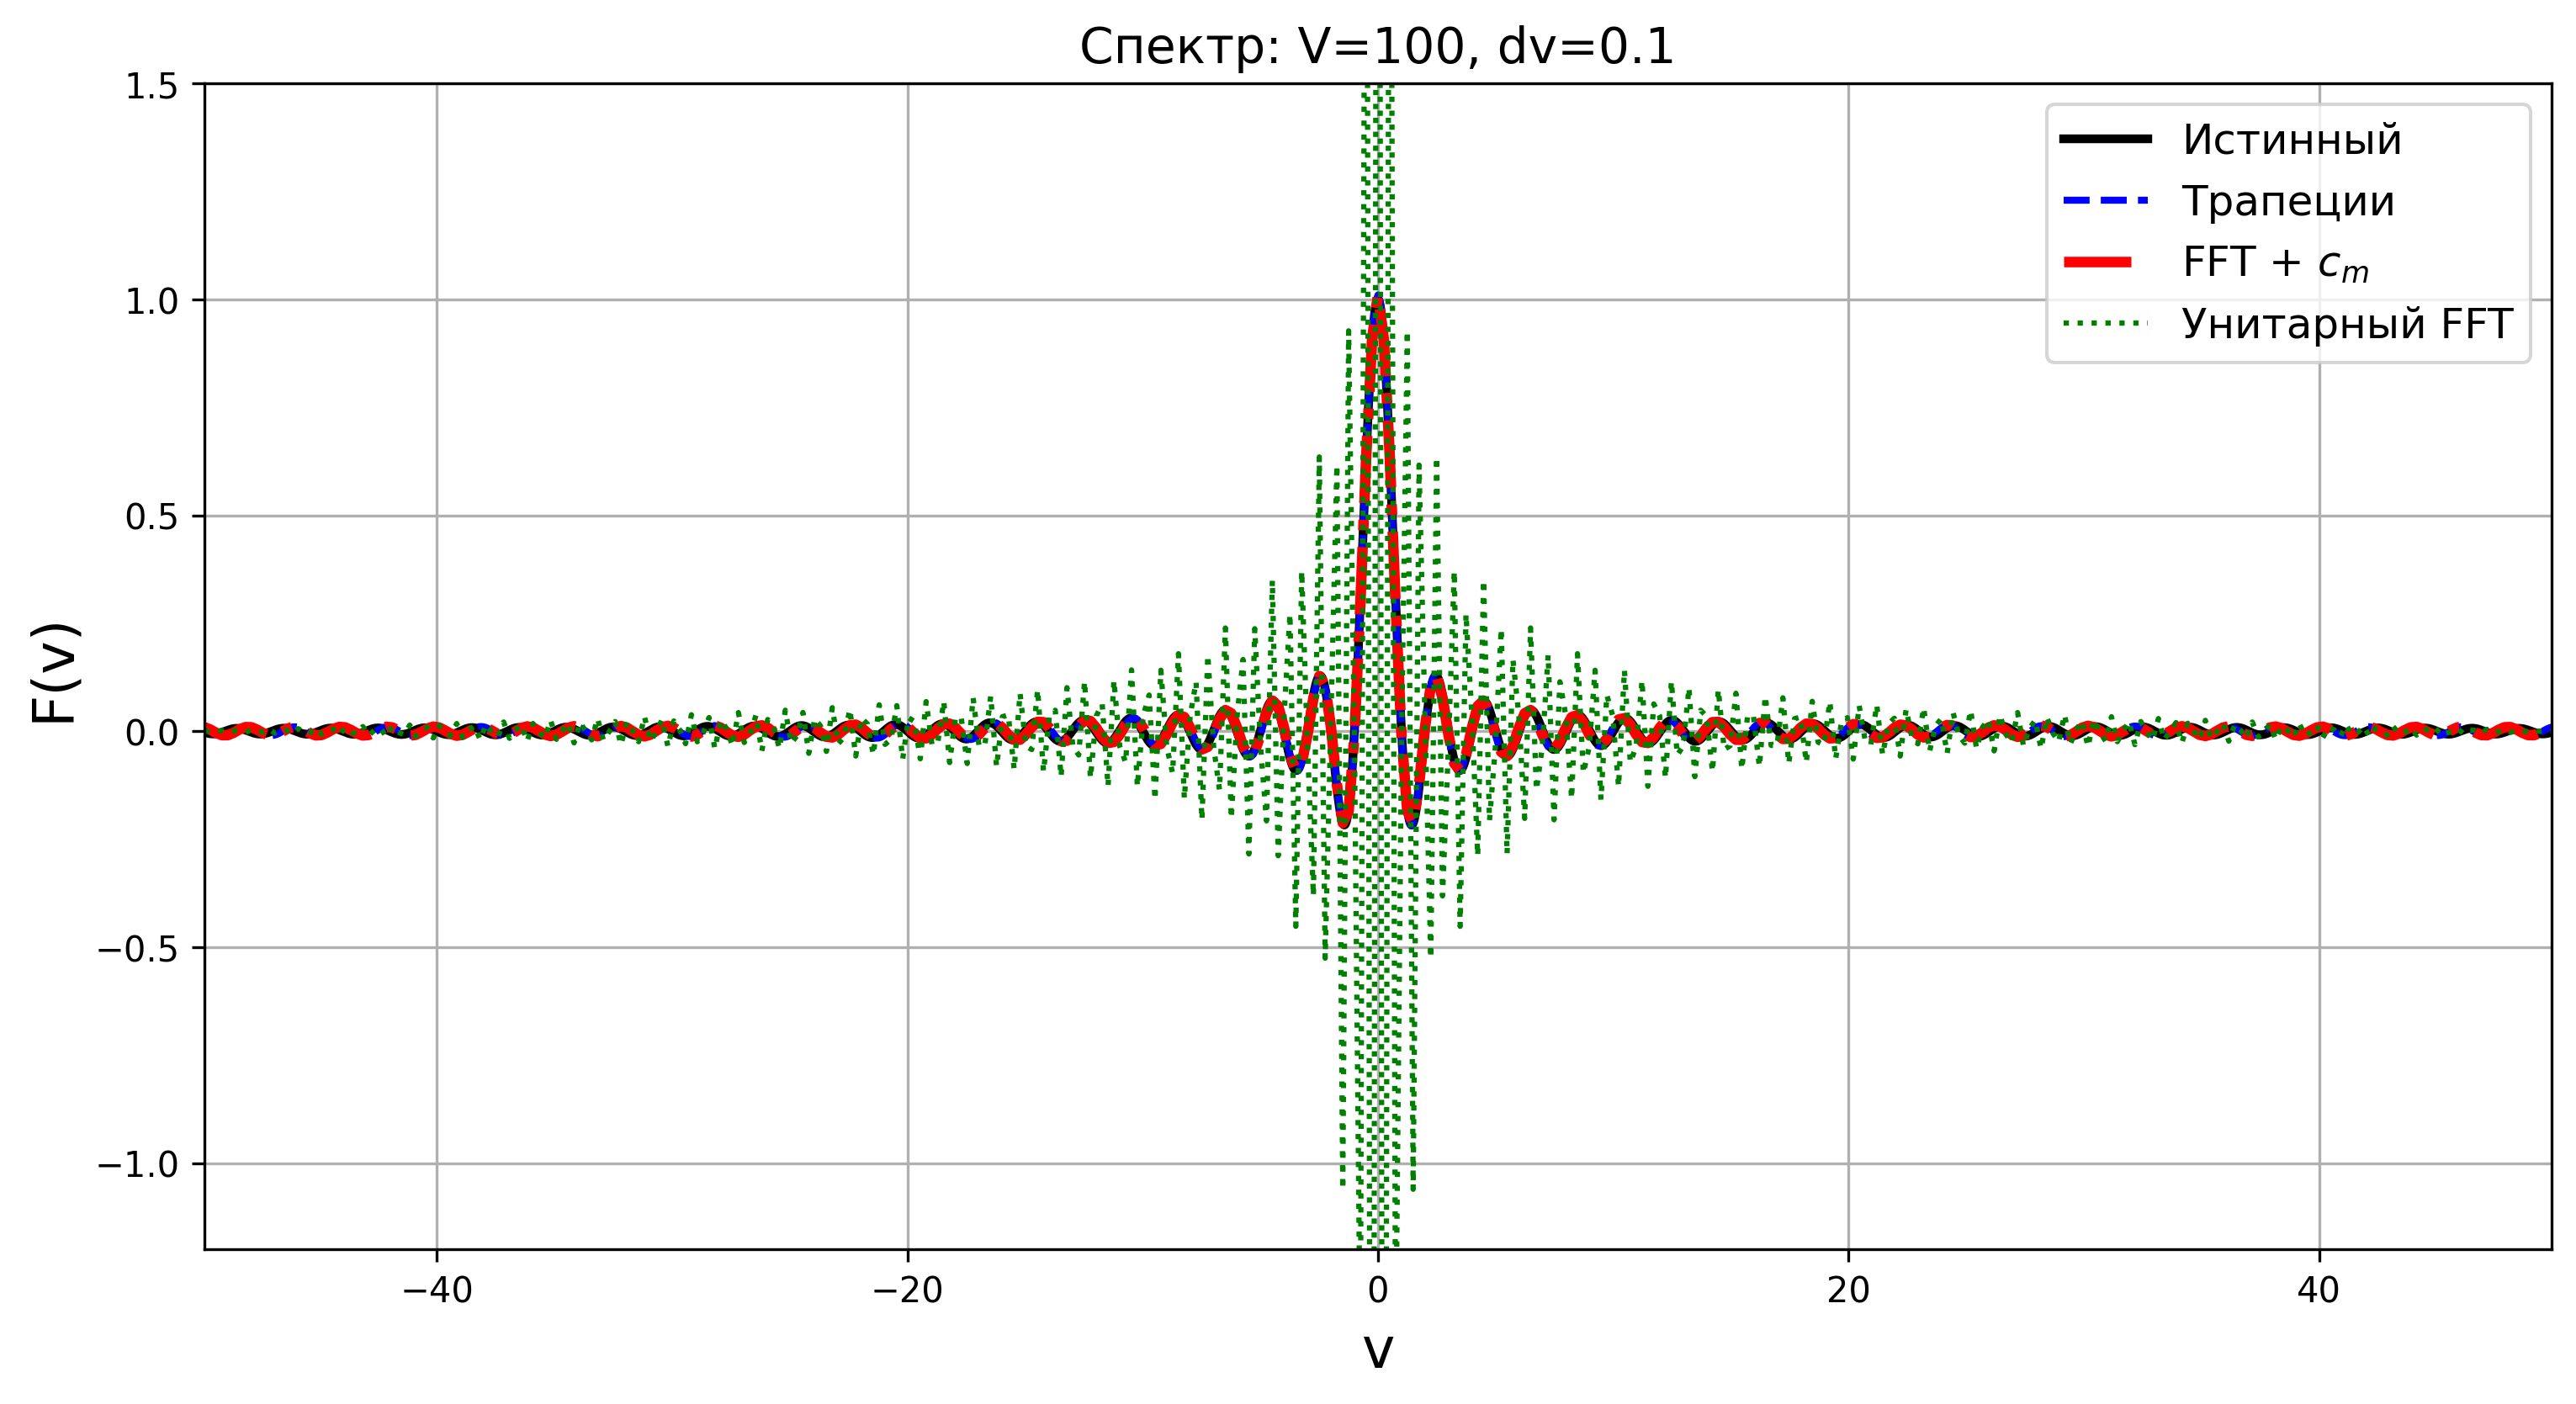
\includegraphics[width=0.95\textwidth]{images/ALL_T4_V100_dt0.010_dv0.100_spectrum.png}
    \caption{Сравнение спектров: $V=100$, $dv=0.1$.}
\end{figure}


\newpage
\subsection*{Комбинация 2: $T=4$, $V=200$, $dt=0.01$, $dv=0.1$}

\begin{figure}[H]
    \centering
    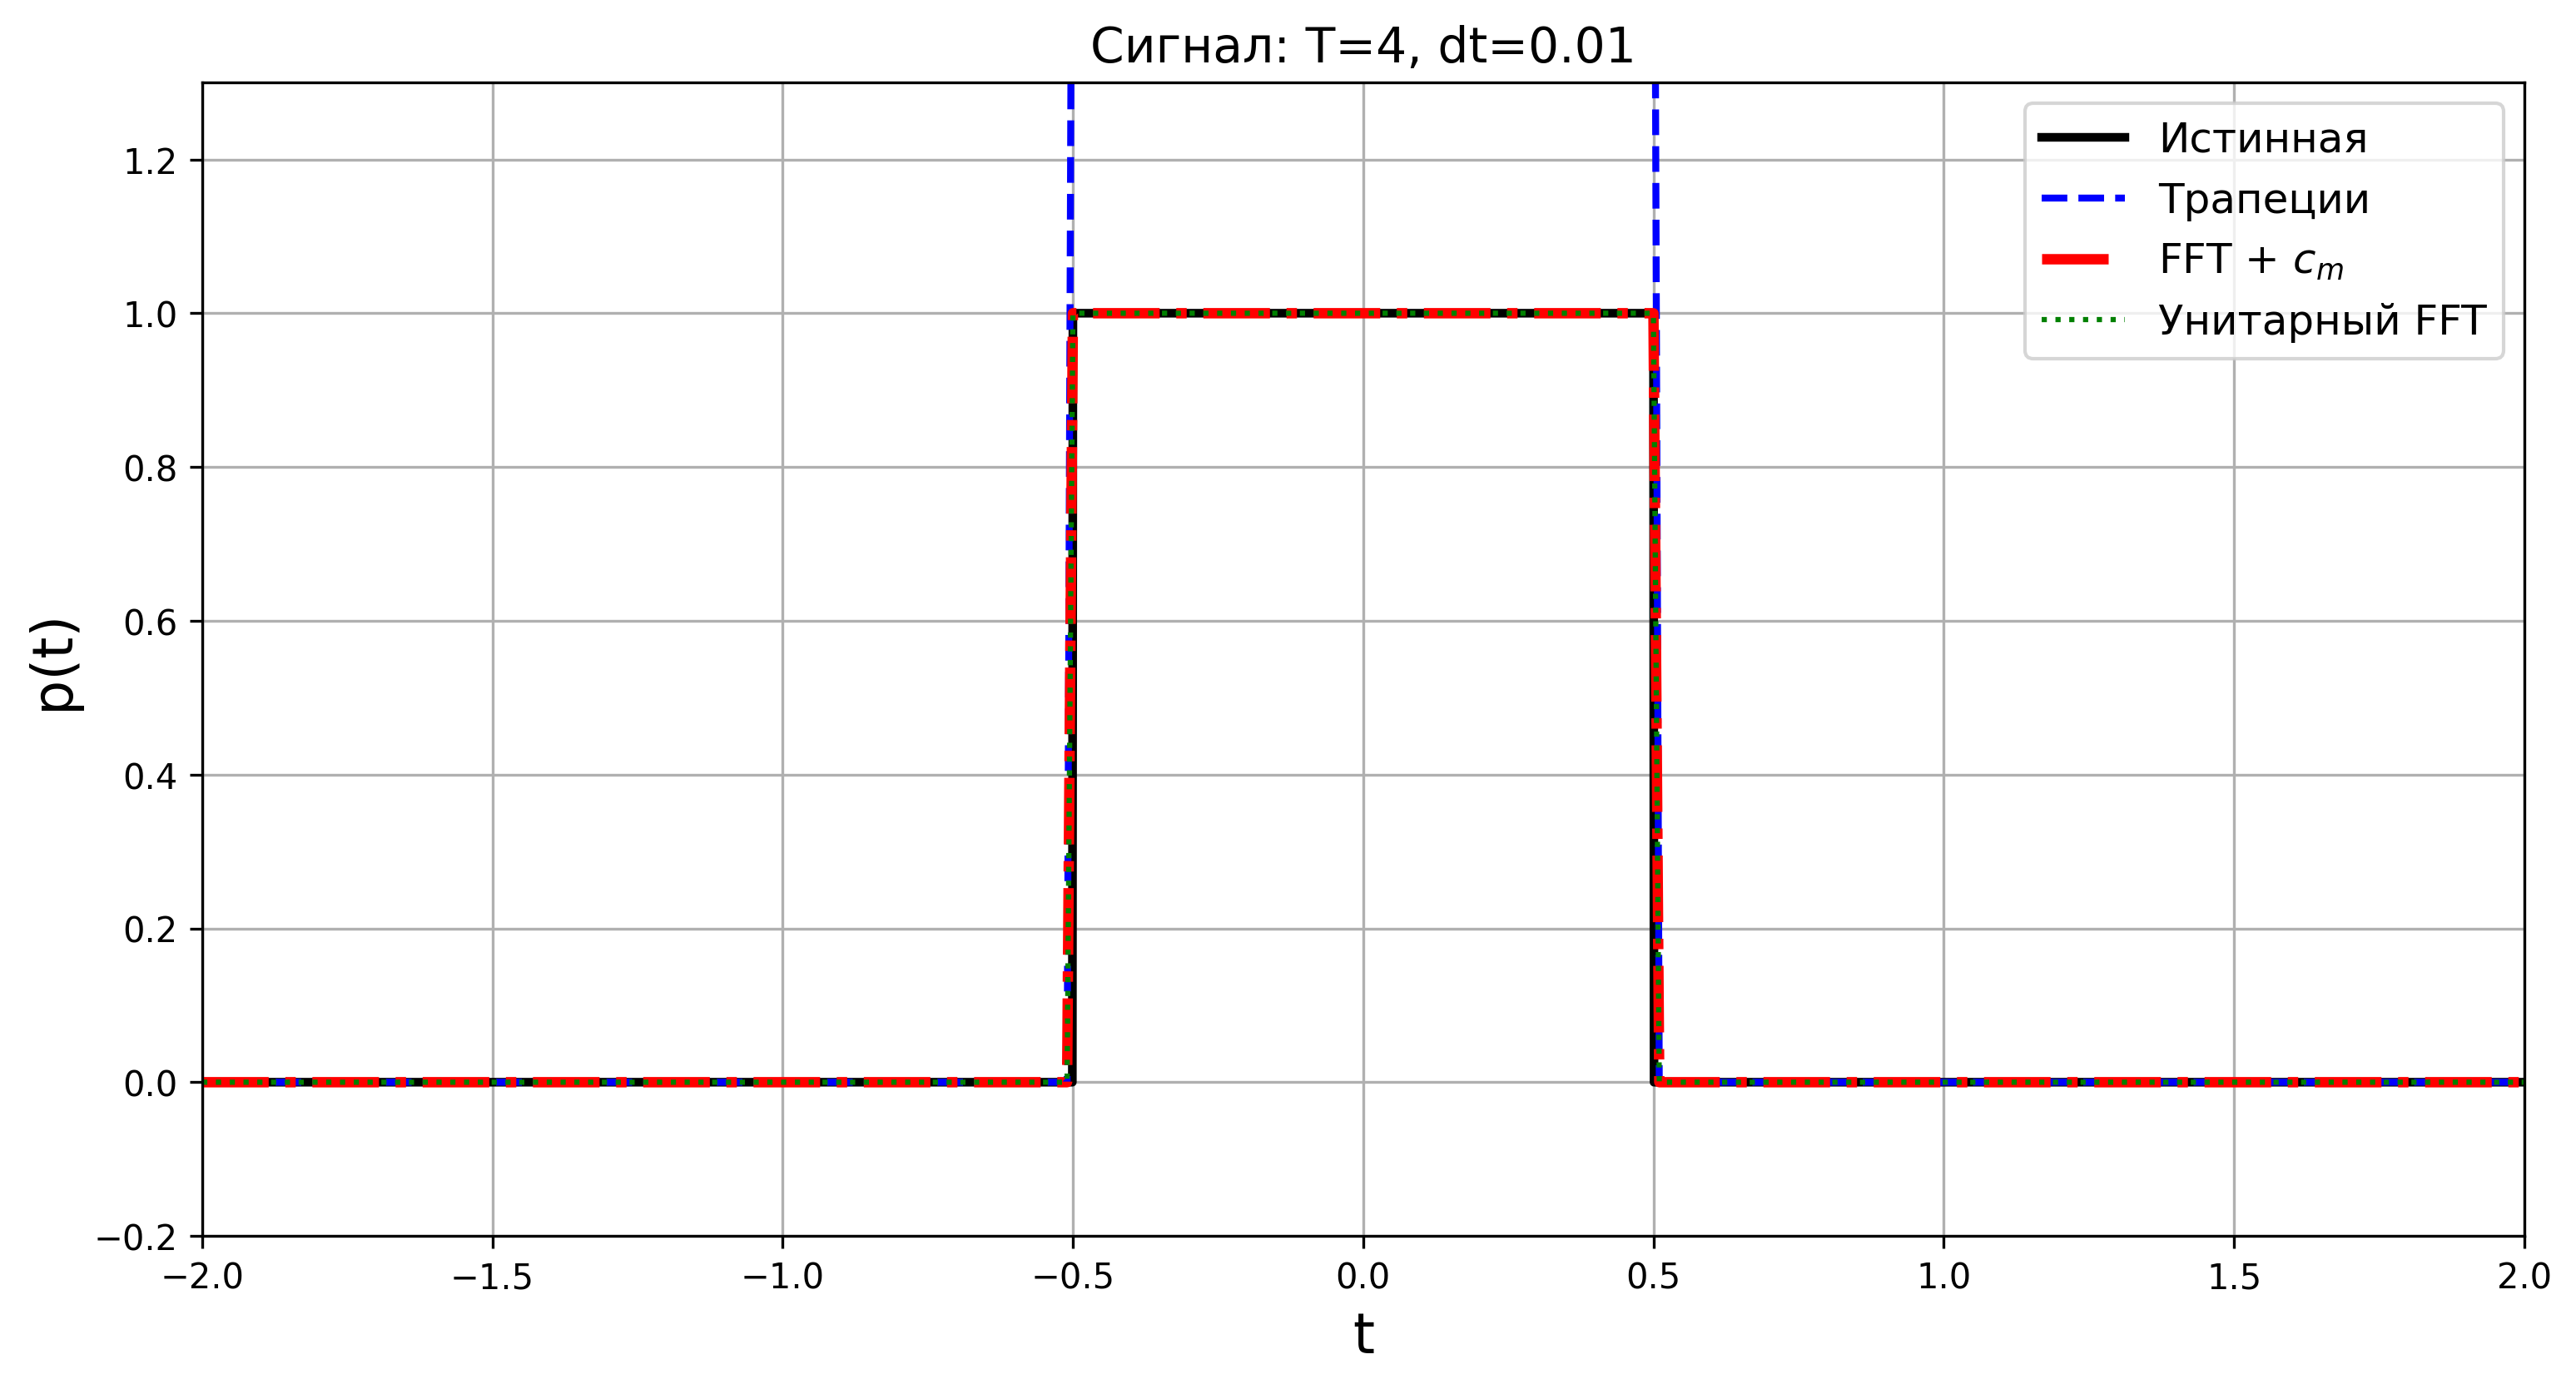
\includegraphics[width=0.95\textwidth]{images/ALL_T4_V200_dt0.010_dv0.100_signal.png}
    \caption{Восстановление сигнала: $T=4$, $dt=0.01$.}
\end{figure}

\begin{figure}[H]
    \centering
    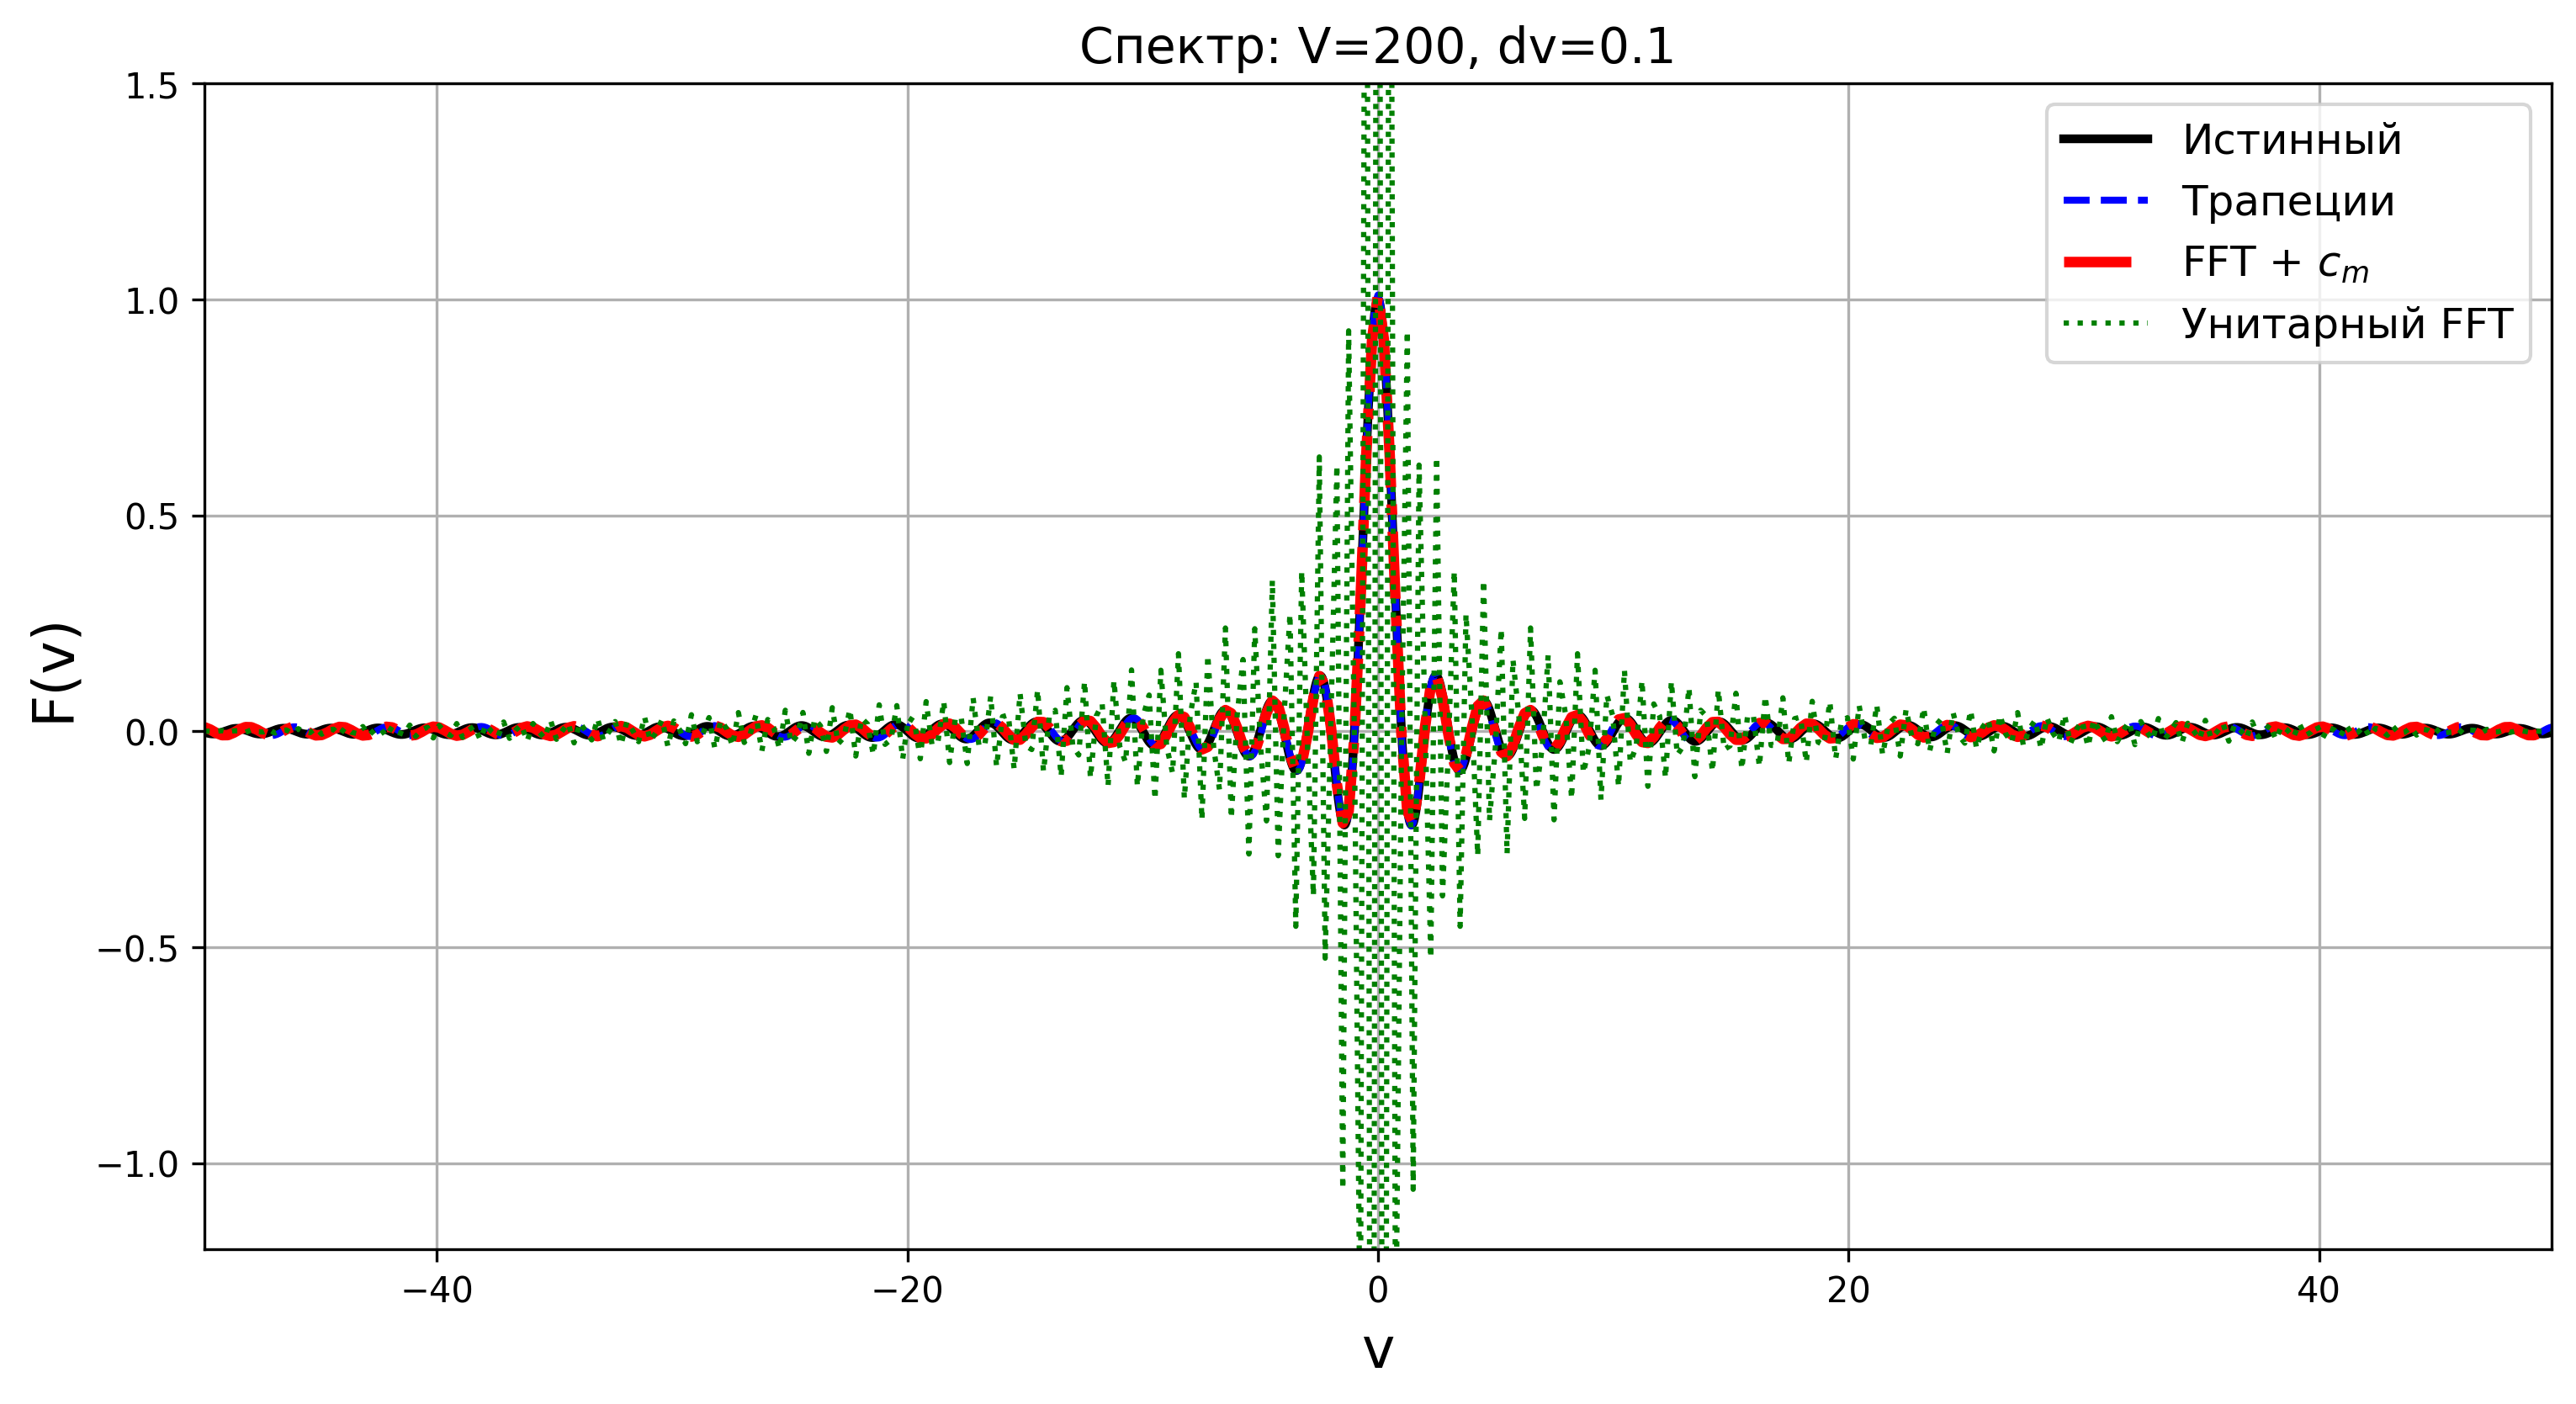
\includegraphics[width=0.95\textwidth]{images/ALL_T4_V200_dt0.010_dv0.100_spectrum.png}
    \caption{Сравнение спектров: $V=200$, $dv=0.1$.}
\end{figure}

\newpage
\subsection*{Комбинация 3: $T=4$, $V=100$, $dt=0.1$, $dv=0.1$}

\begin{figure}[H]
    \centering
    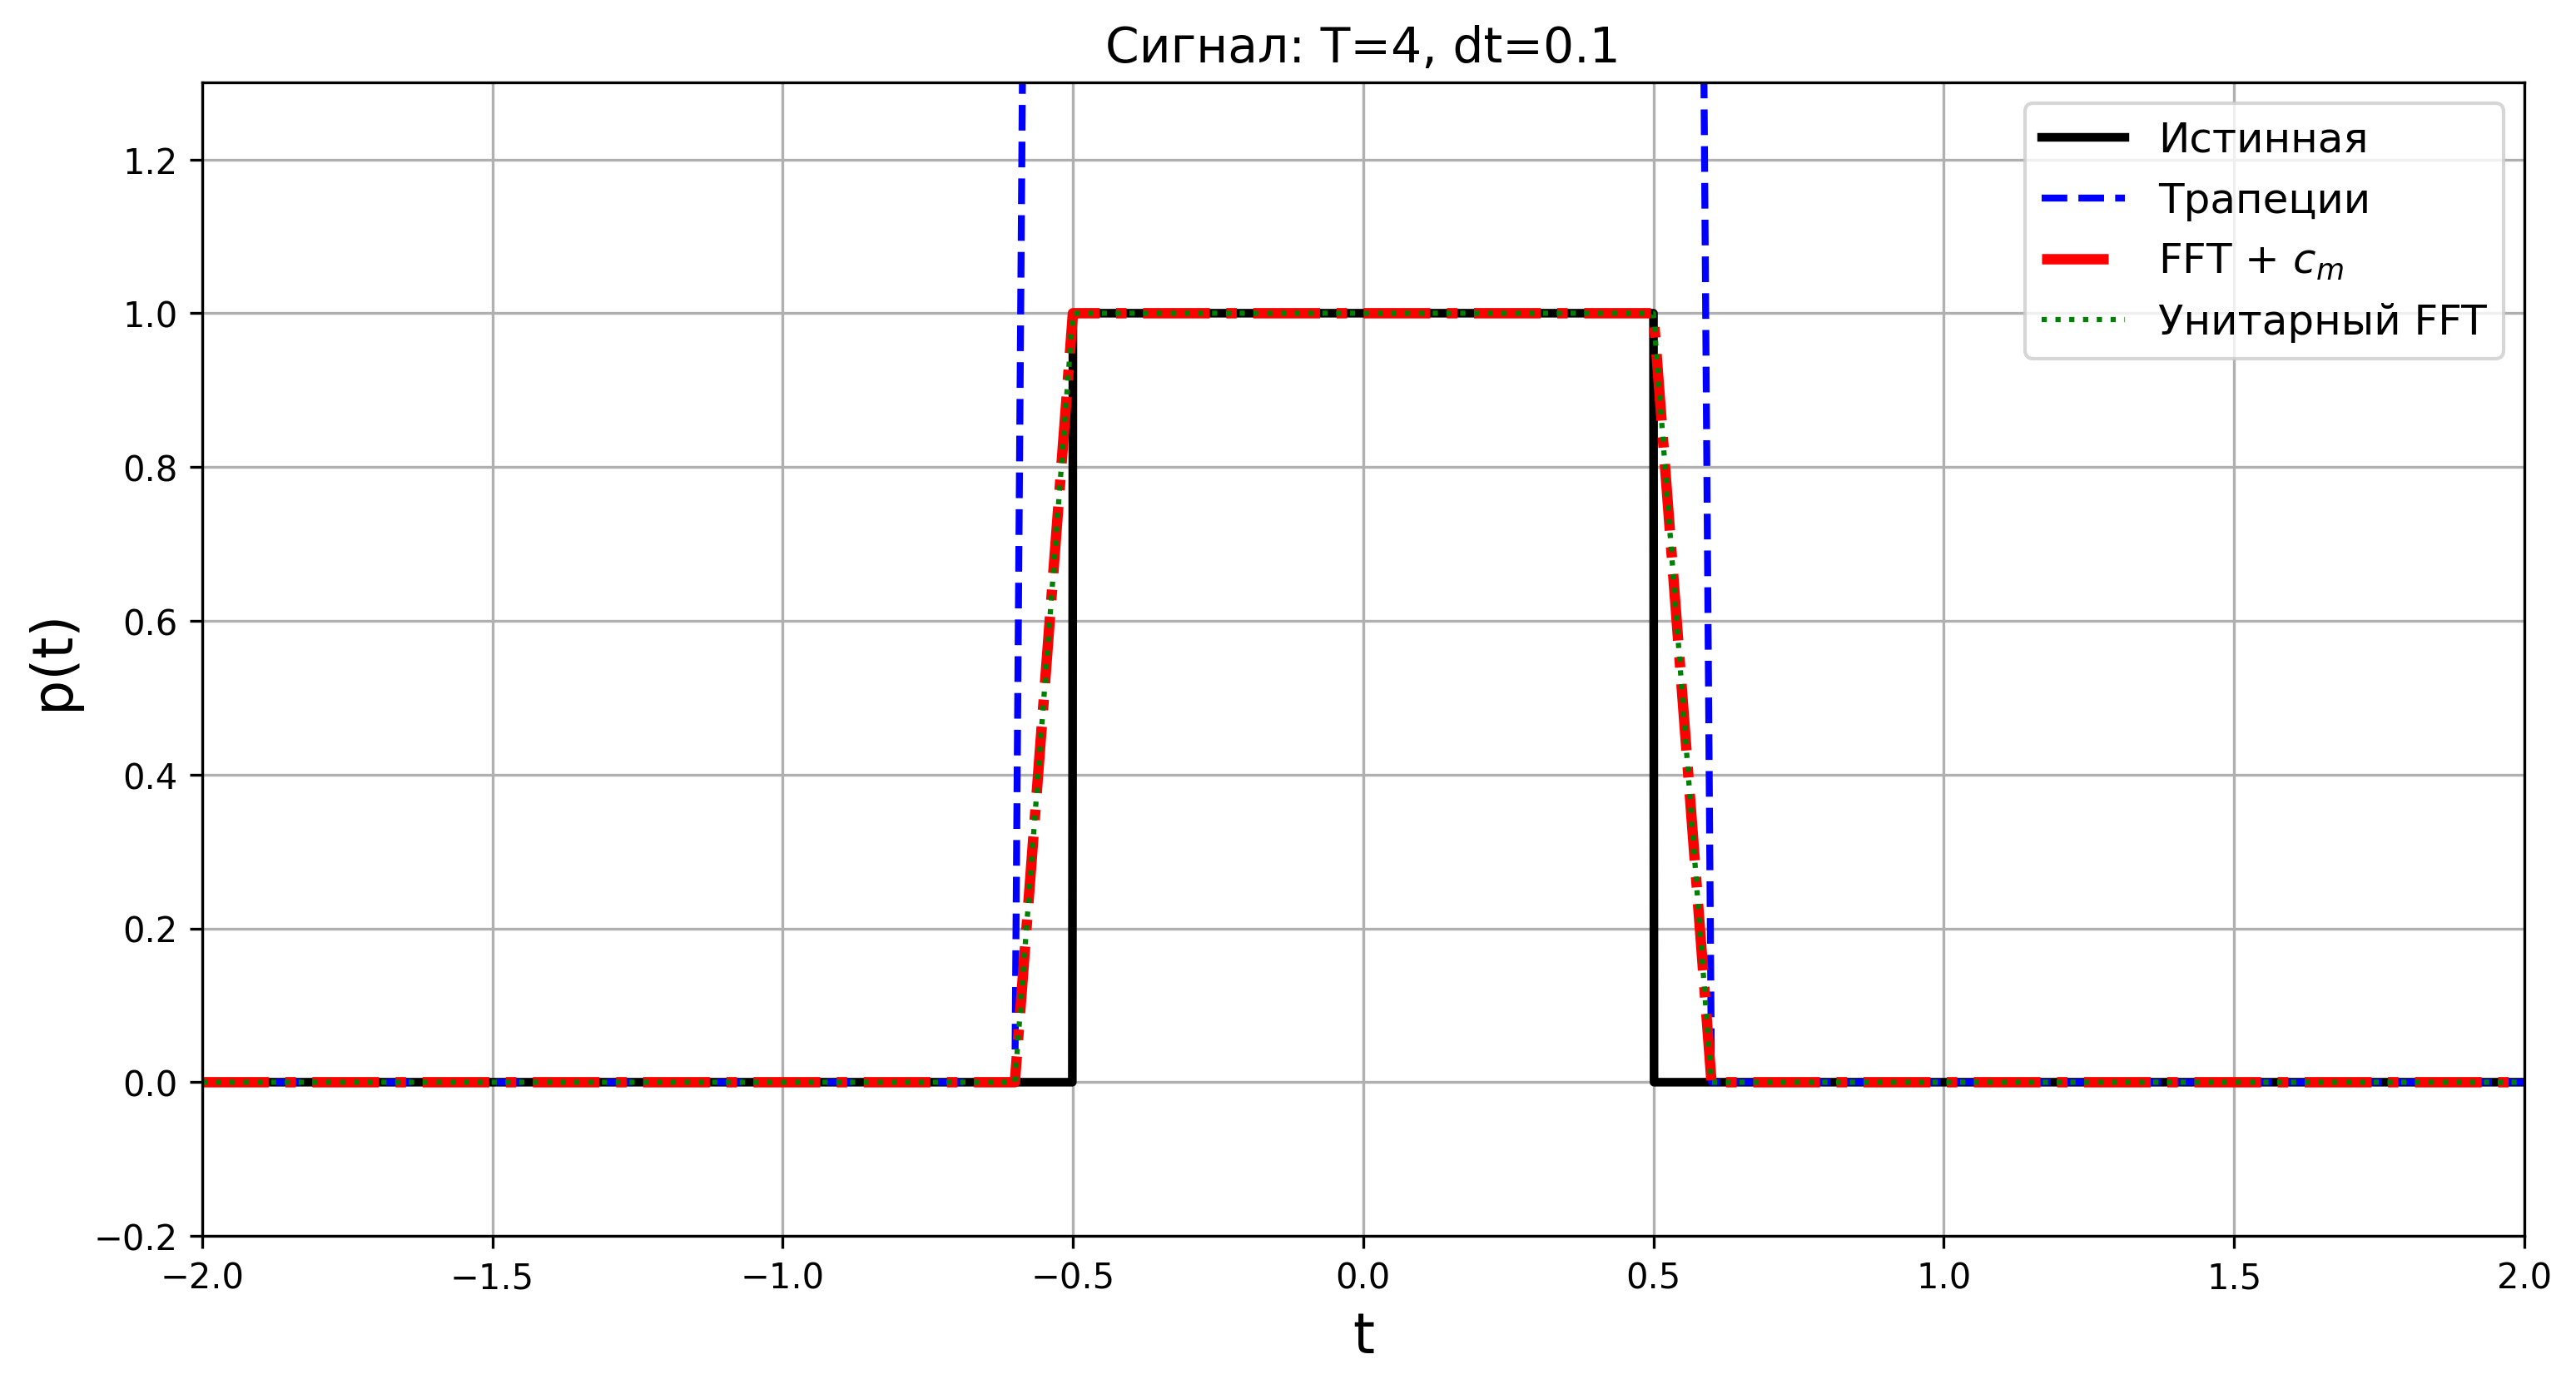
\includegraphics[width=0.95\textwidth]{images/ALL_T4_V100_dt0.100_dv0.100_signal.png}
    \caption{Восстановление сигнала: $T=4$, $dt=0.1$.}
\end{figure}

\begin{figure}[H]
    \centering
    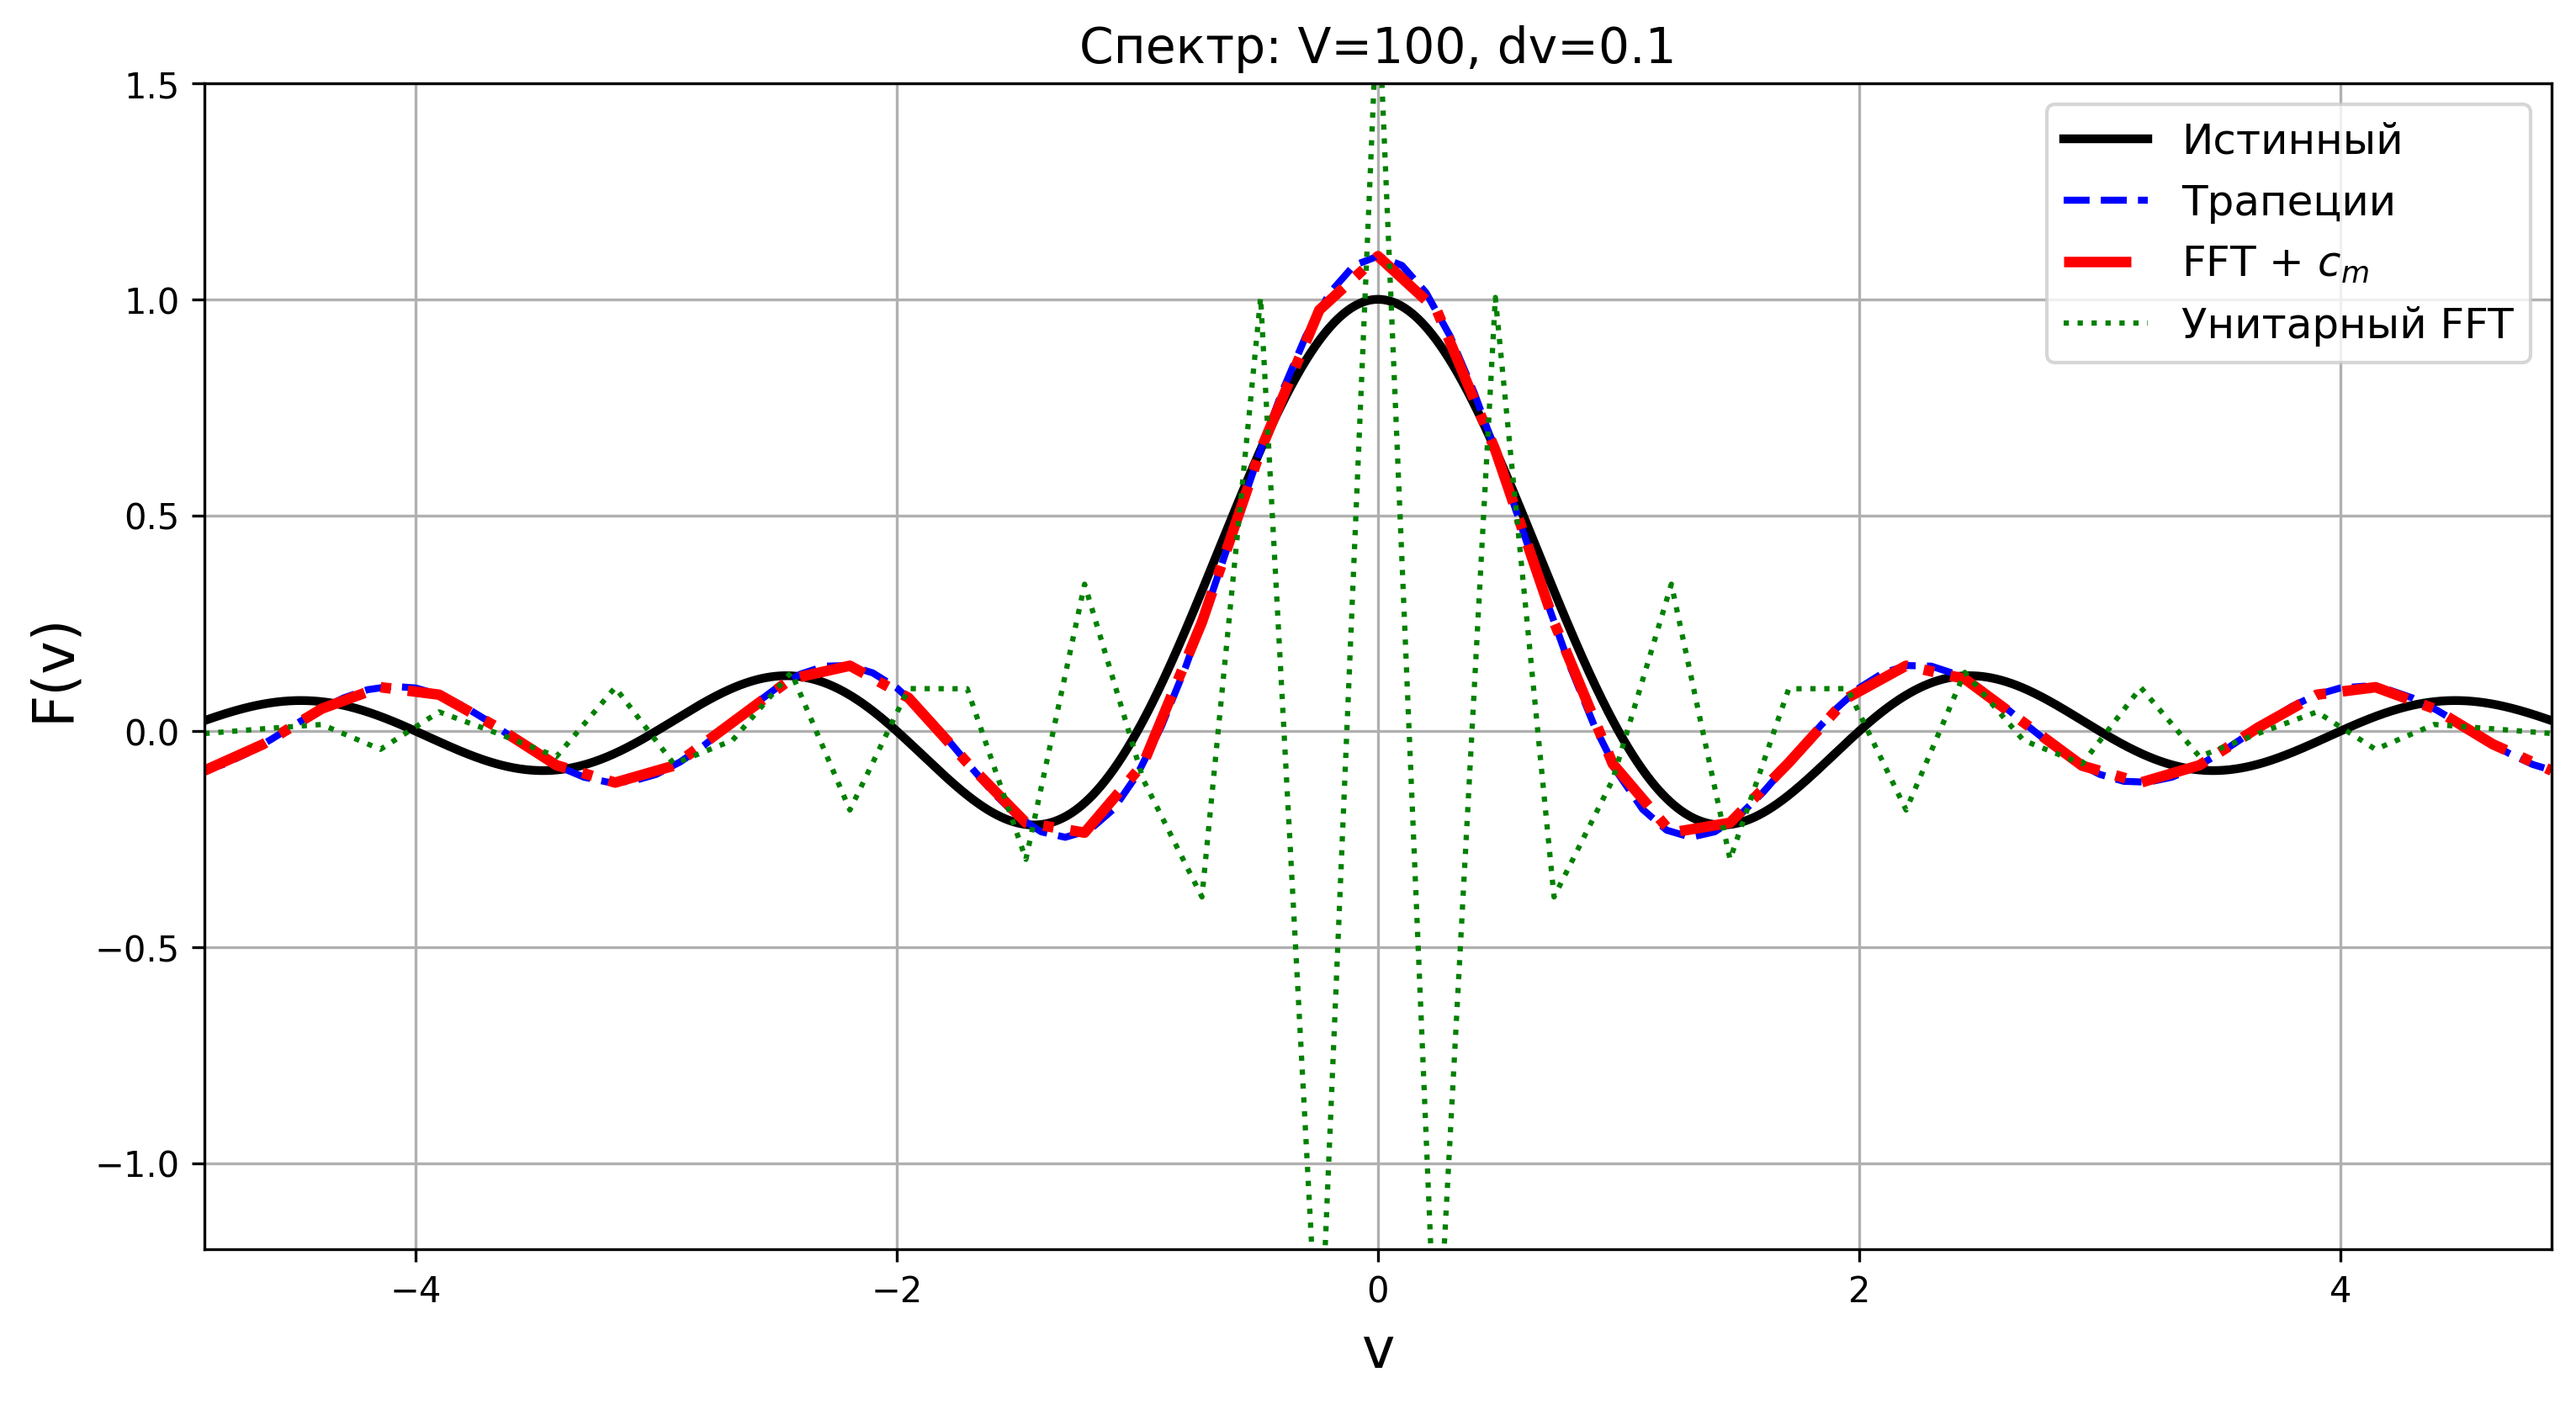
\includegraphics[width=0.95\textwidth]{images/ALL_T4_V100_dt0.100_dv0.100_spectrum.png}
    \caption{Сравнение спектров: $V=100$, $dv=0.1$.}
\end{figure}

\newpage
\subsection*{Комбинация 4: $T=4$, $V=100$, $dt=0.01$, $dv=0.5$}

\begin{figure}[H]
    \centering
    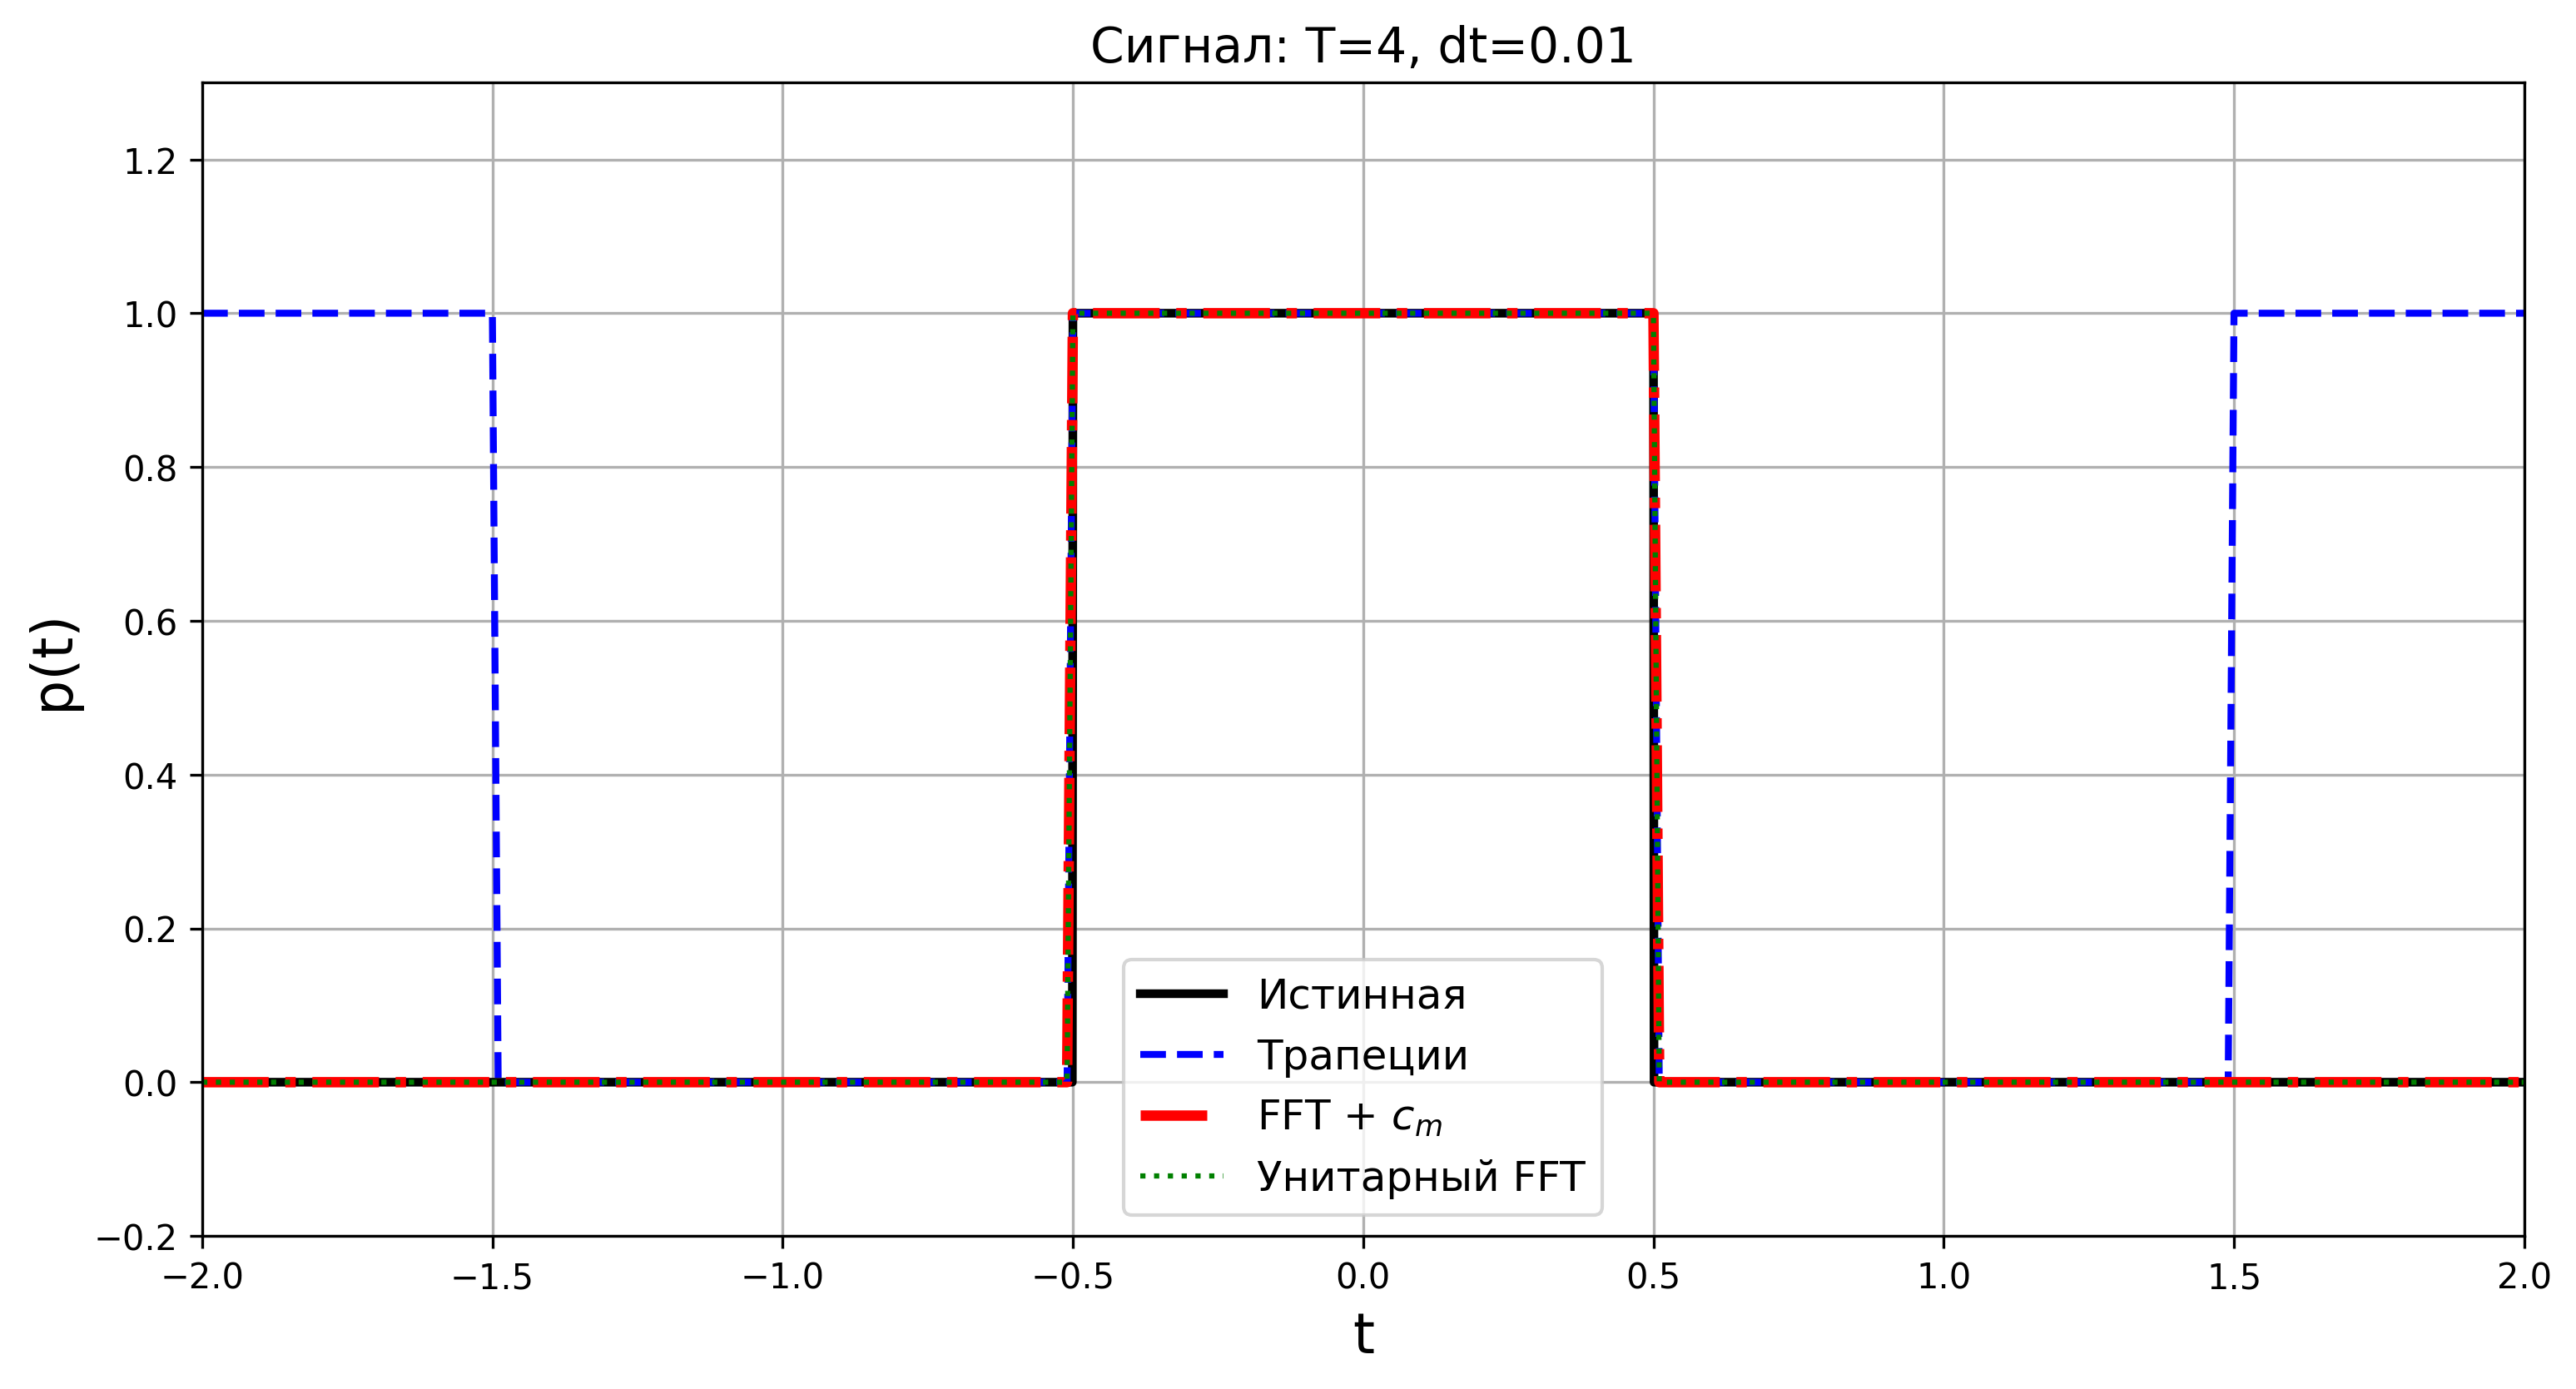
\includegraphics[width=0.95\textwidth]{images/ALL_T4_V100_dt0.010_dv0.500_signal.png}
    \caption{Восстановление сигнала: $T=4$, $dt=0.01$.}
\end{figure}

\begin{figure}[H]
    \centering
    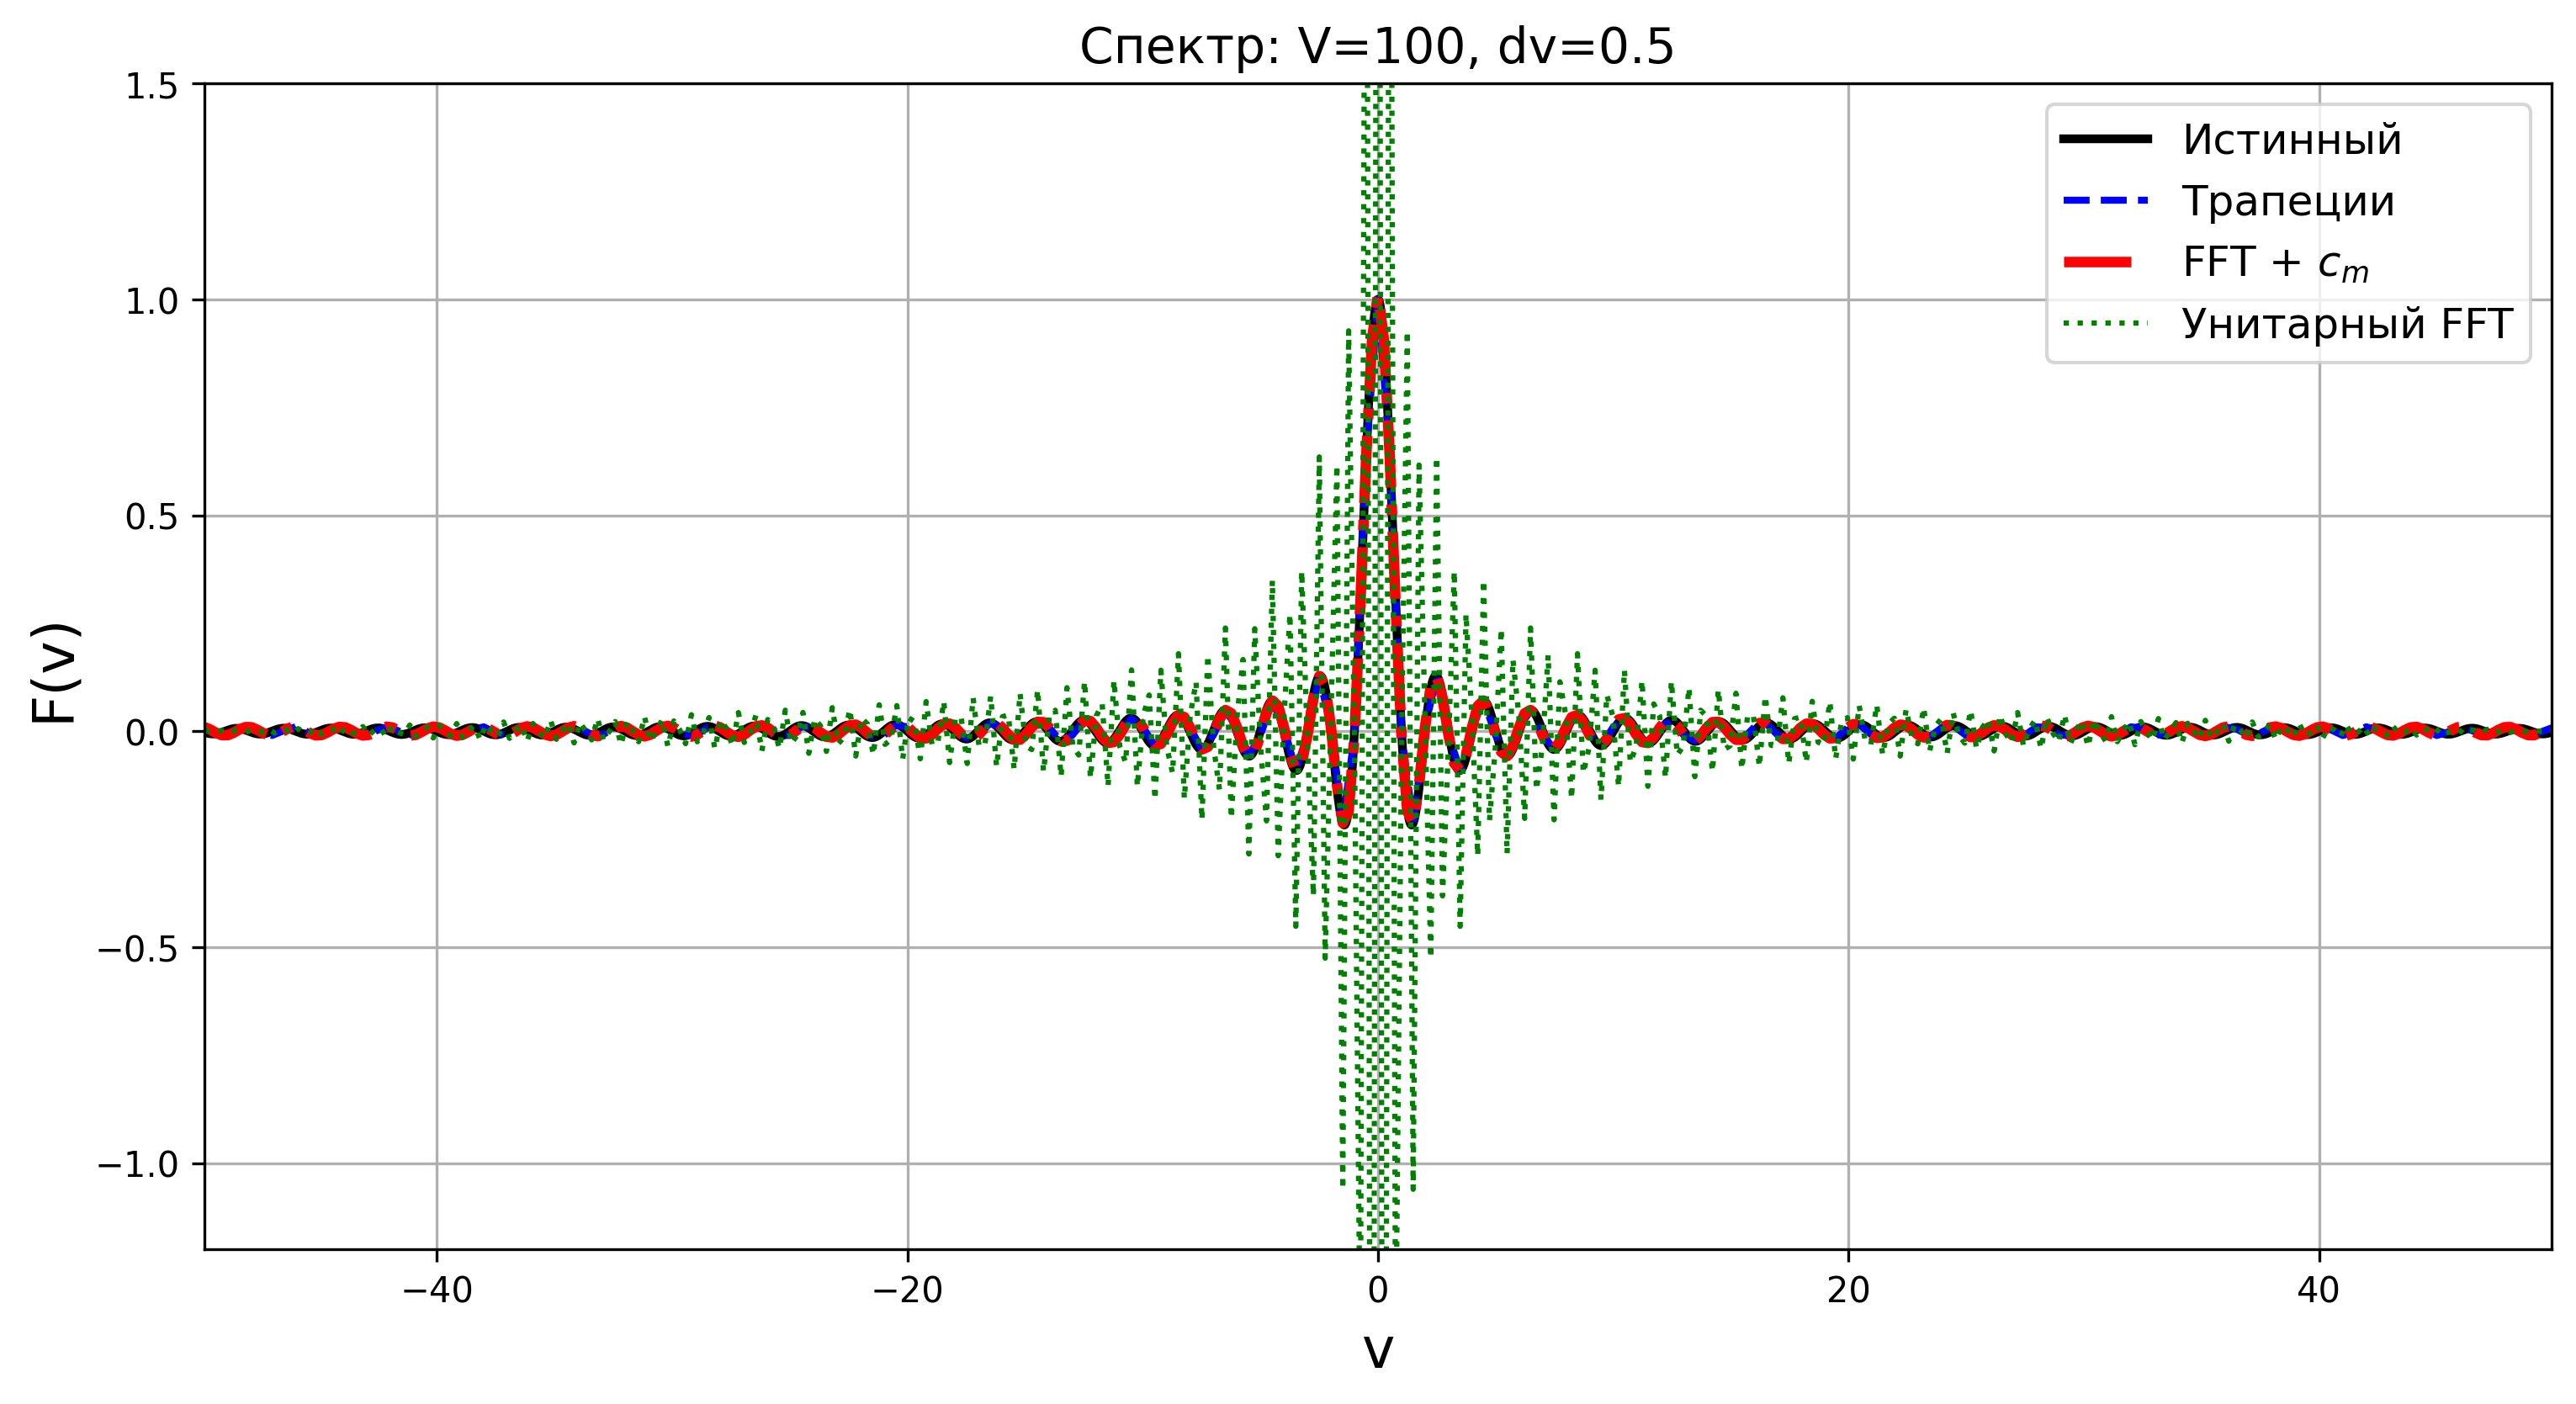
\includegraphics[width=0.95\textwidth]{images/ALL_T4_V100_dt0.010_dv0.500_spectrum.png}
    \caption{Сравнение спектров: $V=100$, $dv=0.5$.}
\end{figure}


Комбинированный метод работает быстрее численного интегрирования и точнее быстрого преобразования. Метод трапеций всегда работает точнее, но и самый затратный по времени.


\newpage
\section{Сэмплирование}
\subsection{Описание задания}
В этом задании мы будем восстанавливать непрерывные функции $y_1(t)$ и $y_2(t)$ по их дискретным значениям с заданной частотой и проиллюстрируем выполнение теоремы Найквиста-Шеннона-Котельникова.
В качестве функции $y_1(t)$ возьмем:
\[
y_1(t) = a_1 sin(\omega_1 t + \varphi_1) + a_2 sin(\omega_2 t + \varphi_2)
\]
Пусть:
\[
a_1 = 1, \omega_1 = 5\pi, \varphi_1 = 11\pi, a_2 = 2, \omega_2 = 3\pi, \varphi_2 = 13\pi
\]
Тогда функция $y_1(t)$ примет вид:
\[
y_1(t) = sin(5 \pi t + 11\pi) + 2 sin(3 \pi t + 13\pi)
\]
В качестве функции $y_2(t)$ возьмем:
\[
y_2(t) = sinc(bt)
\]
Пусть:
\[
b = 7
\]
Тогда функция $y_2(t)$ примет вид:
\[
y_2(t) = sinc(7t)
\]
Непрерывный сигнал из дискретного восстанавливается по формуле:
\[
y(t) = \sum_{n = -\infty}^{\infty} y(n\Delta t) \cdot sinc(\frac{t - n\Delta t}{\Delta t})
\]
По теореме Найквиста-Шеннона-Котельникова функция может быть восстановлена из дискретного набора точек с любой точностью если частота дискретизации $\Delta t \leq \frac{1}{2B}$.
\newline
Для функции $y_1(t)$:
\[
B = \frac{max(\omega_1, \omega_2)}{2\pi} = 2.5 => \Delta t \leq \frac{1}{5}
\]
Для функции $y_2(t)$:
\[
B = \frac{b}{2} = 3.5 => \Delta t \leq \frac{1}{7}
\]
\newpage
\subsection{Анализ функции $y_1(t)$}
Построим график "непрерывной" функции $y_1(t)$. Для этого вычислим значения функции $y_1(t)$ при $-100 \leq t \leq 100$, c шагом $\frac{1}{100}$. Построим график на отрезке $-3 \leq t \leq 3$:
\begin{figure}[H]
    \centering
    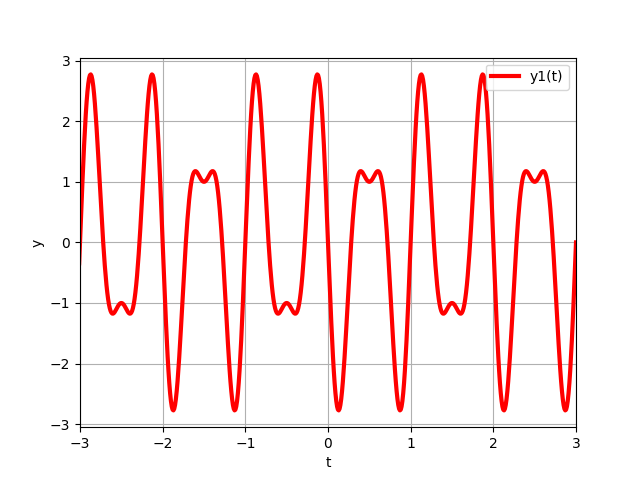
\includegraphics[width=0.75\textwidth]{images2/y1nepr.png}
    \caption{График $y1(t)$ без видимой дискретизации}
\end{figure}

Рассмотрим восстановление функции $y_1(t)$ из дискретной при различных параметрах $T, \Delta t$ (считаем что при данном $T$ интегрируем на промежутке $[-T, T]$):
\begin{figure}[H]
    \centering
    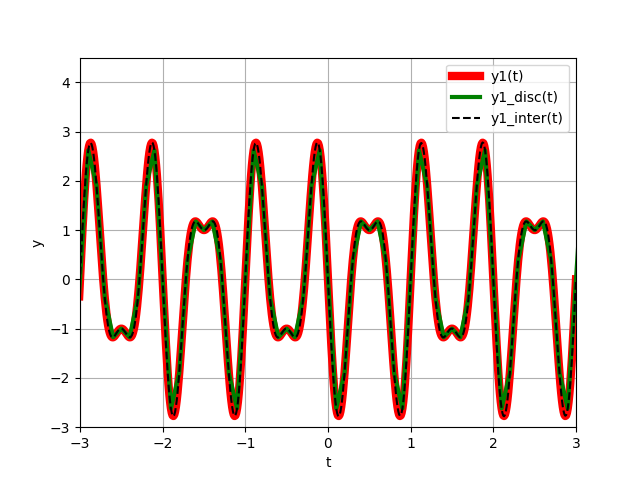
\includegraphics[width=0.75\textwidth]{images2/y1_T10_dt01.png}
    \caption{$T = 10, \Delta t = 0.1$}
\end{figure}
\newpage
\begin{figure}[H]
    \centering
    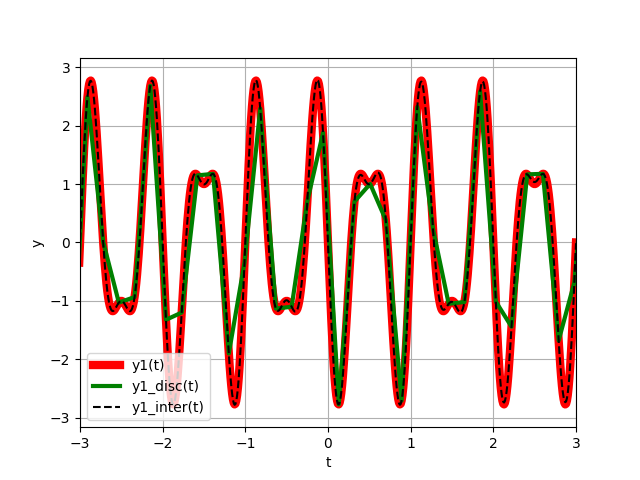
\includegraphics[width=0.85\textwidth]{images2/y1_T10_dt019.png}
    \caption{$T = 10, \Delta t = 0.19$}
\end{figure}
\begin{figure}[H]
    \centering
    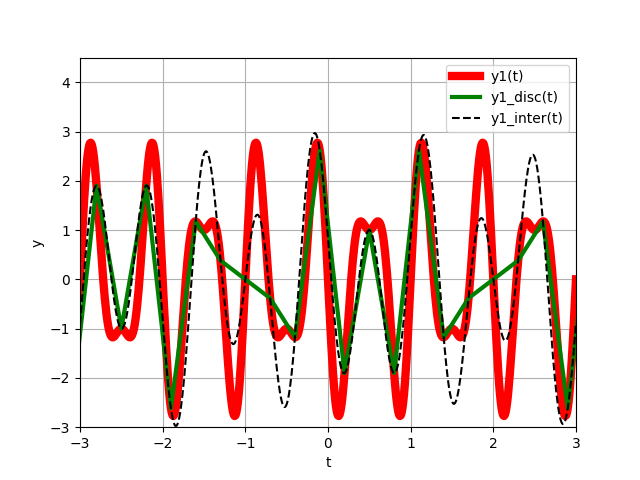
\includegraphics[width=0.85\textwidth]{images2/y1_T10_dt03.png}
    \caption{$T = 10, \Delta t = 0.3$}
\end{figure}
\newpage
\begin{figure}[H]
    \centering
    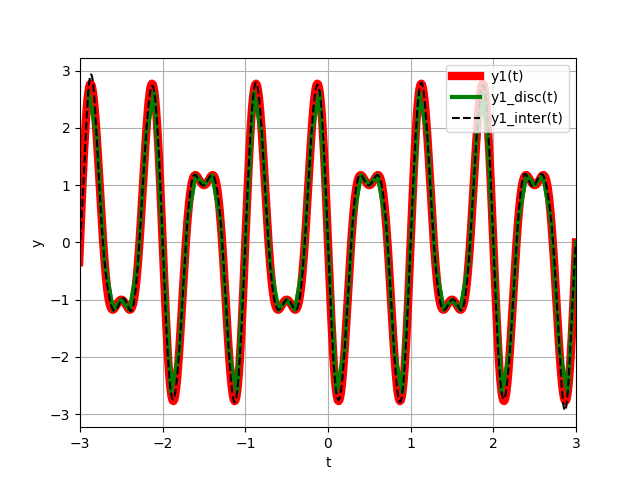
\includegraphics[width=0.85\textwidth]{images2/y1_T3_dt01.png}
    \caption{$T = 3, \Delta t = 0.1$}
\end{figure}
\begin{figure}[H]
    \centering
    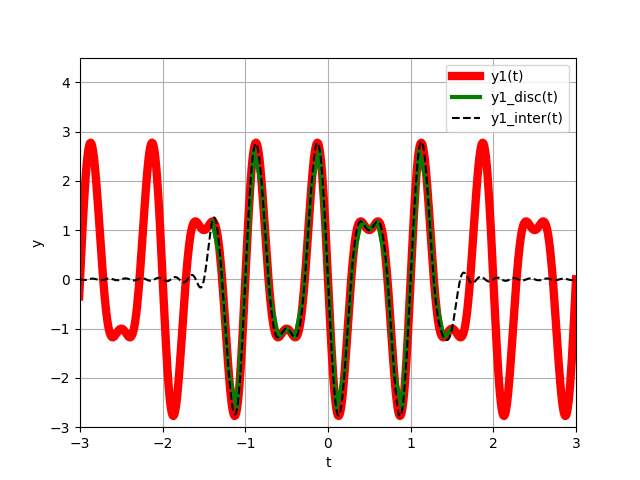
\includegraphics[width=0.85\textwidth]{images2/y1_T15_dt01.png}
    \caption{$T = 1.5, \Delta t = 0.1$}
\end{figure}
\newpage
Также рассмотрим модули Фурье-образов этих функций при данных $T, \Delta t$:
\begin{figure}[H]
    \centering
    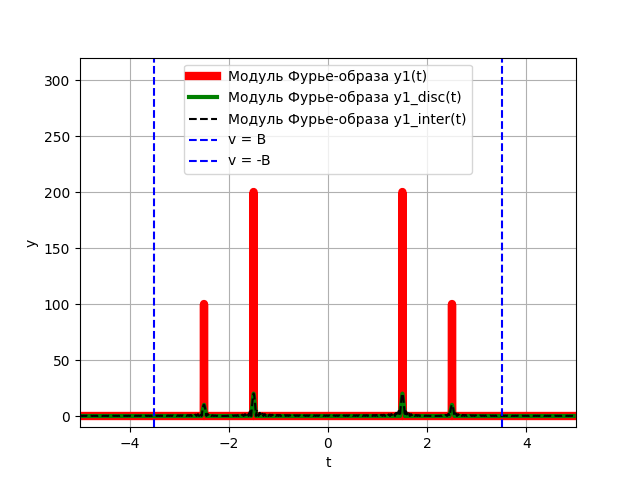
\includegraphics[width=0.80\textwidth]{images2/fur_y1_T10_dt01.png}
    \caption{$T = 10, \Delta t = 0.1$}
\end{figure}
\begin{figure}[H]
    \centering
    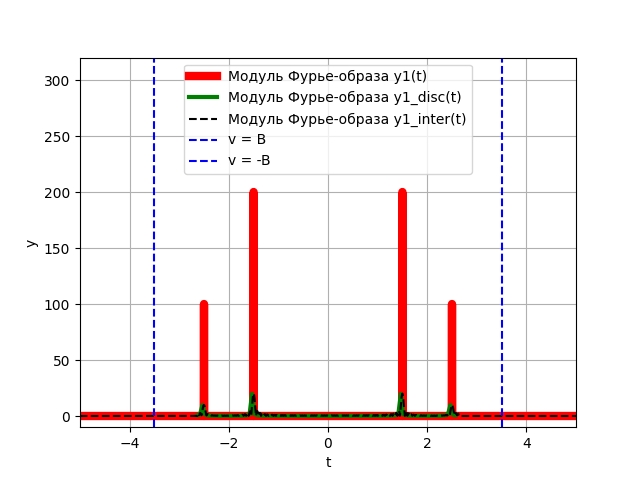
\includegraphics[width=0.80\textwidth]{images2/fur_y1_T10_dt019.png}
    \caption{$T = 10, \Delta t = 0.19$}
\end{figure}
\newpage
\begin{figure}[H]
    \centering
    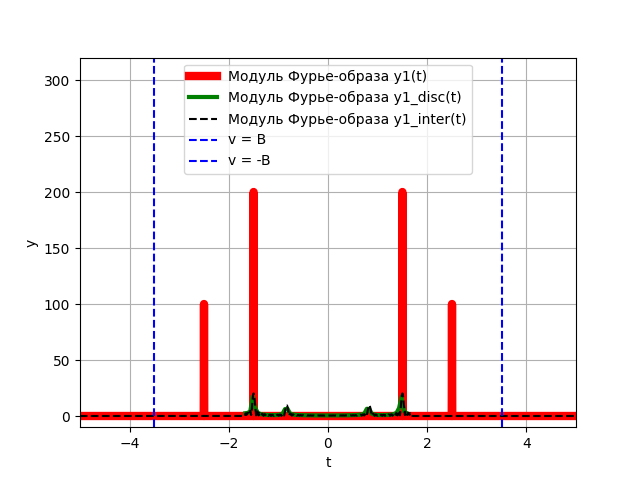
\includegraphics[width=0.85\textwidth]{images2/fur_y1_T10_dt03.png}
    \caption{$T = 10, \Delta t = 0.3$}
\end{figure}
\begin{figure}[H]
    \centering
    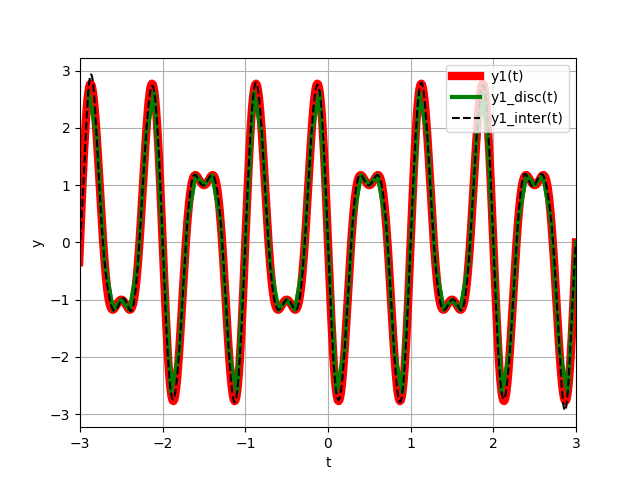
\includegraphics[width=0.85\textwidth]{images2/y1_T3_dt01.png}
    \caption{$T = 3, \Delta t = 0.1$}
\end{figure}
\newpage
\begin{figure}[H]
    \centering
    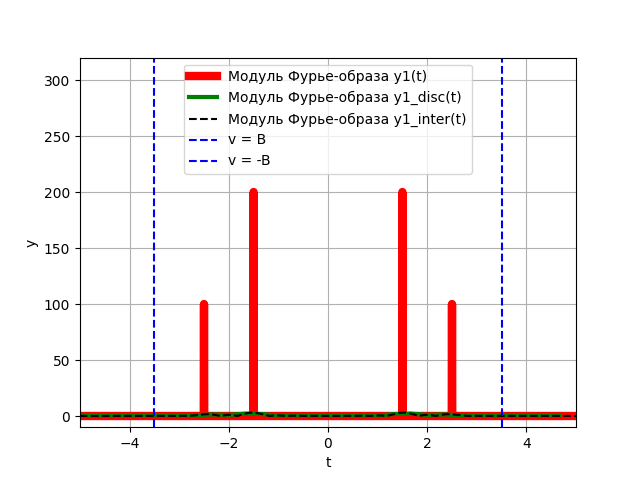
\includegraphics[width=0.75\textwidth]{images2/fur_y1_T15_dt01.png}
    \caption{$T = 1.5, \Delta t = 0.1$}
\end{figure}
\subsection{Анализ функции $y_2(t)$}
Аналогично построим графики для функции $y_2(t)$:
Рассмотрим восстановление функции $y_1(t)$ из дискретной при различных параметрах $T, \Delta t$:
\begin{figure}[H]
    \centering
    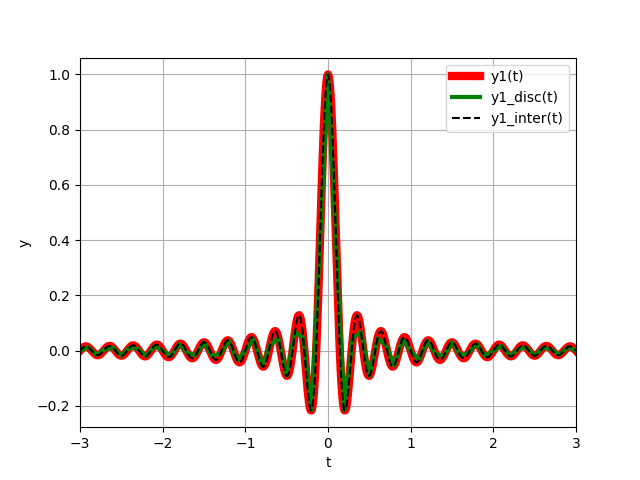
\includegraphics[width=0.75\textwidth]{images2/y2_T10_dt01.png}
    \caption{$T = 10, \Delta t = 0.1$}
\end{figure}
\newpage
\begin{figure}[H]
    \centering
    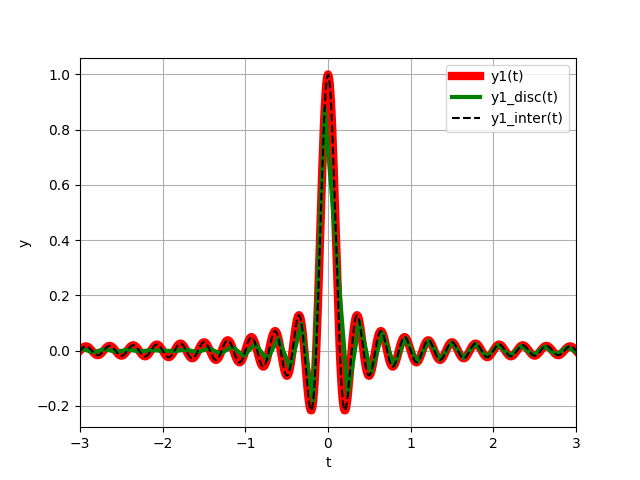
\includegraphics[width=0.85\textwidth]{images2/y2_T10_dt014.png}
    \caption{$T = 10, \Delta t = 0.14$}
\end{figure}
\begin{figure}[H]
    \centering
    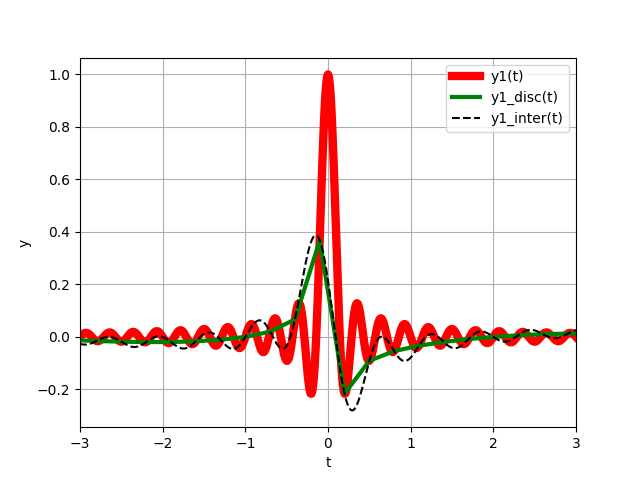
\includegraphics[width=0.85\textwidth]{images2/y2_T10_dt03.png}
    \caption{$T = 10, \Delta t = 0.3$}
\end{figure}
\newpage
\begin{figure}[H]
    \centering
    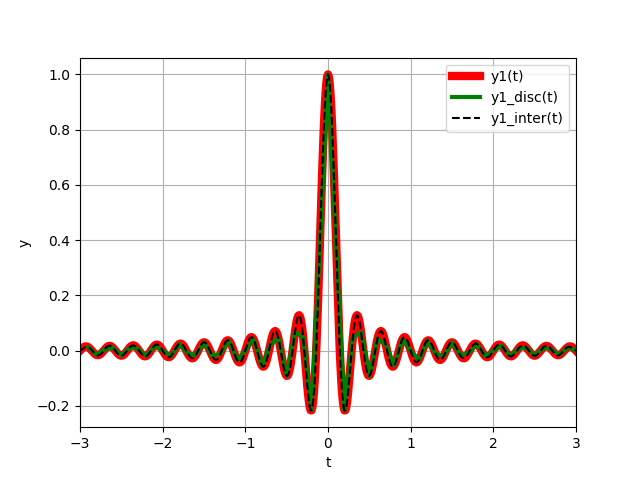
\includegraphics[width=0.85\textwidth]{images2/y2_T3_dt01.png}
    \caption{$T = 3, \Delta t = 0.1$}
\end{figure}
\begin{figure}[H]
    \centering
    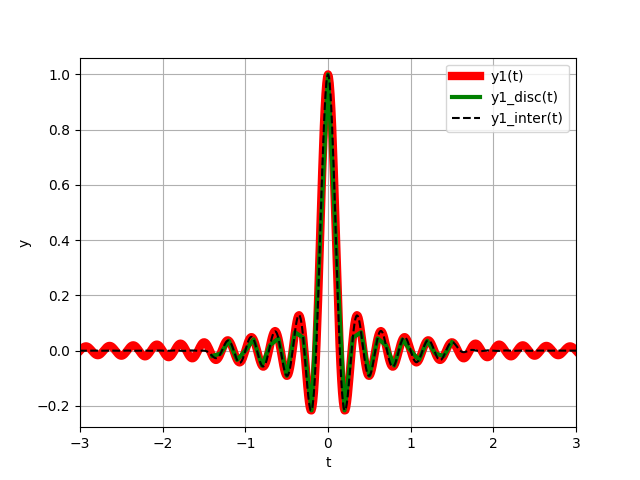
\includegraphics[width=0.85\textwidth]{images2/y2_T15_dt01.png}
    \caption{$T = 1.5, \Delta t = 0.1$}
\end{figure}
\newpage
Также рассмотрим модули Фурье-образов этих функций при данных $T, \Delta t$:
\begin{figure}[H]
    \centering
    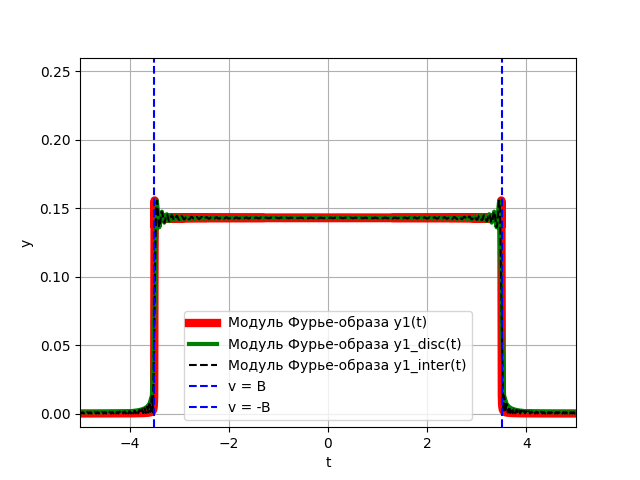
\includegraphics[width=0.80\textwidth]{images2/fur_y2_T10_dt01.png}
    \caption{$T = 10, \Delta t = 0.1$}
\end{figure}
\begin{figure}[H]
    \centering
    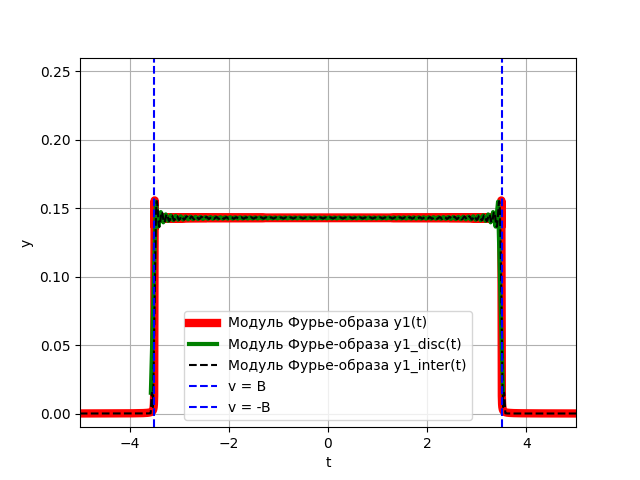
\includegraphics[width=0.80\textwidth]{images2/fur_y2_T10_dt014.png}
    \caption{$T = 10, \Delta t = 0.14$}
\end{figure}
\newpage
\begin{figure}[H]
    \centering
    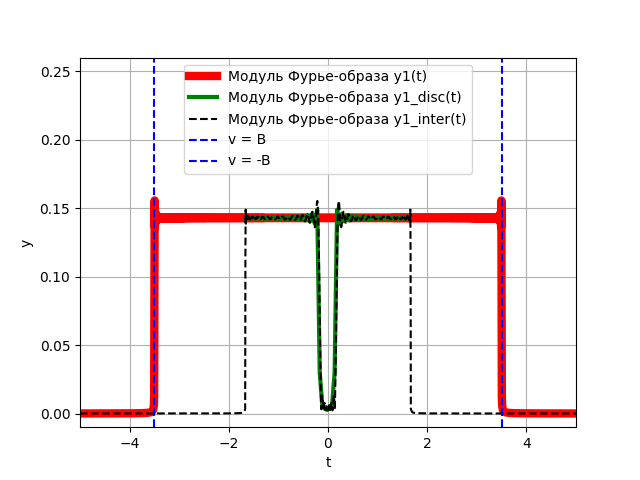
\includegraphics[width=0.85\textwidth]{images2/fur_y2_T10_dt03.png}
    \caption{$T = 10, \Delta t = 0.3$}
\end{figure}
\begin{figure}[H]
    \centering
    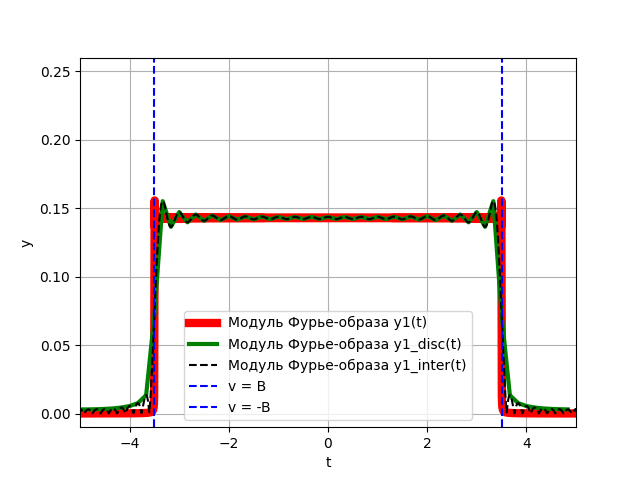
\includegraphics[width=0.85\textwidth]{images2/fur_y2_T3_dt01.png}
    \caption{$T = 3, \Delta t = 0.1$}
\end{figure}
\newpage
\begin{figure}[H]
    \centering
    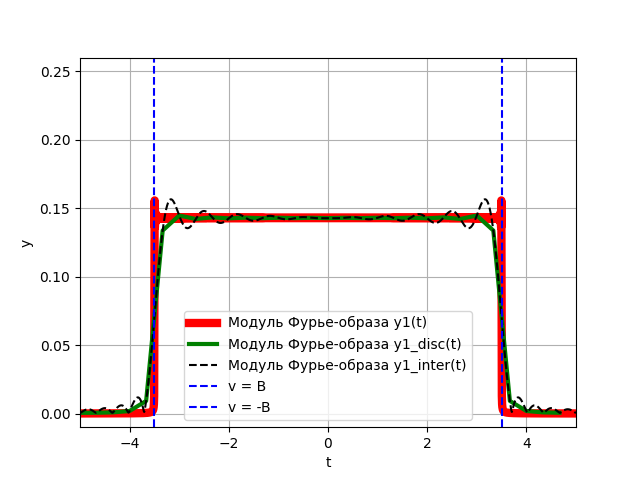
\includegraphics[width=0.75\textwidth]{images2/fur_y2_T15_dt01.png}
    \caption{$T = 1.5, \Delta t = 0.1$}
\end{figure}
\subsection{Выводы}
Видим, что при $\Delta t \leq \frac{1}{2B}$ функция полученная с помощью интерполяции с высокой точностью соответствует исходной на промежутке интегрирования $T$. Если же $\Delta t > \frac{1}{2B}$, восстанавливаемая функция значительно отличается от исходной. Данный результат полностью соответствует теореме Найквиста-Шеннона-Котельникова.
\newline
Параметр $T$ (промежуток интегрирования) соответствует промежутку на котором интерполированная функция восстанавливается с высокой точностью, на остальной же числовой прямой функция после интерполяции быстро стремится к нулю.
\newline
При рассмотрении же Фурье-образов можно заметить что Фурье-образ восстановленной функции совпадает с Фурье-образом исходной функции с меньшей точностью при уменьшении $T$ (шаг дискретизации частоты зависит от промежутка интегрирования как $\Delta \nu = \frac{1}{2T}$).
\newpage


\section{Вывод}
В данной работе мы рассмотрели различные способы вычисления Фурье-образа прямоугольной функции (аналитически, с помощью численного интегрирования и с помощью дискретного преобразования Фурье двумя способами). Таким образом был получен комбинированный способ, учитывающий недостатки каждого из способов, таким образом получаем быстрое преобразование Фурье, которое получает образ, близкий к истинному.
Кроме того, было получен, что основной критерий, отвечающий за совпадение образа и функции, восстановленной из него, с истинной, есть частота разбиения частотной и временной областей.
\newline
Также было выполнено восстановление функций из дискретного набора значений и проиллюстрировано выполнение теоремы Найквиста-Шеннона-Котельникова. Что также показывает важность мелкости разбиения временной и частотной шкал, и даёт оценку, необходимую для правильного восстановления.

\newpage
\section{Приложения}
\begin{lstlisting}[caption={Код для численного интегрирования в первом пункте}]
import numpy as np
import matplotlib.pyplot as plt
import os

trapz = getattr(np, 'trapezoid', np.trapz)
out_dir = os.path.join('lab5', 'Paper', 'images')

dt_t = 0.001
dv_t = 0.001

combos = [[4, 100, 0.01, 0.1], [15, 100, 0.01, 0.1], [4, 200, 0.01, 0.1], [4, 100, 0.1, 0.1], [4, 100, 0.01, 0.5] ]
for idx, (T, V, dt, dv) in enumerate(combos, 1):

    Nt = int(T / dt) + 1
    Nt_true = int(T / dt_t) + 1
    Nv = int(V / dv) + 1
    Nv_true = int(V / dv_t) + 1
    t = np.linspace(-T/2, T/2, Nt)
    t_true = np.linspace(-T/2, T/2, Nt_true)
    v = np.linspace(-V/2, V/2, Nv)
    v_t = np.linspace(-V/2, V/2, Nv_true)

    p = np.where(np.abs(t) <= 0.5, 1.0, 0.0)
    p_true = np.where(np.abs(t_true) <= 0.5, 1.0, 0.0)

    p_f = (np.exp(-1j * np.pi * v_t) - np.exp(1j * np.pi * v_t)) / (-2j * np.pi * v_t)
    p_f[np.abs(v_t) < dv_t/2] = 1.0

    kernel = np.exp(-2j * np.pi * np.outer(v, t))
    integrand = p[np.newaxis, :] * kernel
    trap_im = trapz(integrand, x=t, axis=1)

    kernel2 = np.exp(2j * np.pi * np.outer(v, t))
    integrand_inv = trap_im[:, np.newaxis] * kernel2
    p_rev = trapz(integrand_inv, x=v, axis=0)
    p_rev = np.real(p_rev)

    fig1, ax1 = plt.subplots(figsize=(12, 6))
    ax1.plot(t_true, p_true, 'b-', linewidth=2.5, label='Истинная')
    ax1.plot(t, p_rev, 'r--', linewidth=1.5, label='Восстановленная (trapz)')
    ax1.set_xlabel('t', fontsize=16); ax1.set_ylabel('p(t)', fontsize=16)
    ax1.set_title(f'Сигнал: T={T}, dt={dt}', fontsize=14)
    ax1.legend(loc='best', fontsize=16); ax1.grid(True)
    ax1.set_ylim([-0.2, np.max(p_rev)+0.4*np.max(p_rev)])  
    ax1.set_xlim([-T/2, T/2])
    fname1 = f"T{T}_V{V}_dt{dt:.3f}_dv{dv:.3f}_signal.png"
    fig1.savefig(os.path.join(out_dir, fname1), dpi=300, bbox_inches='tight')
    plt.close(fig1)

    fig2, ax2 = plt.subplots(figsize=(12, 6))
    ax2.plot(v_t, np.real(p_f), 'b-', linewidth=2.5, label='Истинный')
    ax2.plot(v, np.real(trap_im), 'r--', linewidth=1.5, label='Численный (trapz)')
    ax2.set_xlabel('v', fontsize=16); ax2.set_ylabel('F(v)', fontsize=16)
    ax2.set_title(f'Спектр: V={V}, dv={dv}', fontsize=14)
    ax2.legend(loc='best', fontsize=16); ax2.grid(True)
    ax2.set_ylim([-0.4, 1.5]); ax2.set_xlim([-V/2, V/2])
    fname2 = f"T{T}_V{V}_dt{dt:.3f}_dv{dv:.3f}_spectrum.png"
    fig2.savefig(os.path.join(out_dir, fname2), dpi=300, bbox_inches='tight')
    plt.close(fig2)

\end{lstlisting}
\begin{lstlisting}[caption={Код для встроенного дискретного преобразования Фурье в первом пункте}]
import numpy as np
import matplotlib.pyplot as plt
import os

out_dir = os.path.join('lab5', 'Paper', 'images')
os.makedirs(out_dir, exist_ok=True)

dt_t = 0.001
dv_t = 0.001

combos = [[4, 100, 0.01, 0.1], [15, 100, 0.01, 0.1], [4, 200, 0.01, 0.1], [4, 100, 0.1, 0.1], [4, 100, 0.01, 0.5] ]
for idx, (T, V, dt, dv) in enumerate(combos, 1):

    V_t = max(V, 100)
    Nt = int(T / dt) + 1
    Nt_true = int(T / dt_t) + 1
    Nv = int(V / dv) + 1
    Nv_true = int(V / dv_t) + 1
    t = np.linspace(-T/2, T/2, Nt)
    t_true = np.linspace(-T/2, T/2, Nt_true)
    v = np.linspace(-V/2, V/2, Nv)
    v_t = np.linspace(-V_t/2, V_t/2, Nv_true)
    dt_actual = dt 
    

    p = np.where(np.abs(t) <= 0.5, 1.0, 0.0)
    p_t = np.where(np.abs(t_true) <= 0.5, 1.0, 0.0)

    F_fft = np.fft.fftshift(np.fft.fft(p)) * (1/np.sqrt(Nt))
    v_fft = np.fft.fftshift(np.fft.fftfreq(Nt, d=dt_actual))
    
    p_f = np.sinc(v_t)

    p_rec = np.fft.ifft(np.fft.ifftshift(F_fft))*np.sqrt(Nt)
    p_rec = np.real(p_rec)

    fig1, ax1 = plt.subplots(figsize=(12, 6))
    ax1.plot(t_true, p_t, 'b-', linewidth=1.5, label='Истинная')
    ax1.plot(t, p_rec, 'r--', linewidth=1.5, label='Восстановленная (FFT)')
    ax1.set_xlabel('t', fontsize=16); ax1.set_ylabel('p(t)', fontsize=16)
    ax1.set_title(f'Сигнал: T={T}, dt={dt}', fontsize=14)
    ax1.legend(loc='best', fontsize=16); ax1.grid(True)
    ax1.set_ylim([-0.2, 1.3])
    ax1.set_xlim([-T/2, T/2])
    fname1 = f"FFT_T{T}_V{V}_dt{dt:.3f}_dv{dv:.3f}_signal.png"
    fig1.savefig(os.path.join(out_dir, fname1), dpi=300, bbox_inches='tight')
    plt.close(fig1)

    fig2, ax2 = plt.subplots(figsize=(12, 6))
    ax2.plot(v_t, np.real(p_f), 'b-', linewidth=3.0, label='Истинный')
    ax2.plot(v_fft, np.real(F_fft), 'r--', linewidth=1.5, label='Численный (FFT)')
    ax2.set_xlabel('v', fontsize=16); ax2.set_ylabel('F(v)', fontsize=16)
    ax2.set_title(f'Спектр: V={V}, dv={dv}', fontsize=14)
    ax2.legend(loc='best', fontsize=16); ax2.grid(True)
    ax2.set_ylim([-1.2, 1.5])
    ax2.set_xlim([-v_fft[-1], v_fft[-1]])
    fname2 = f"FFT_T{T}_V{V}_dt{dt:.3f}_dv{dv:.3f}_spectrum.png"
    fig2.savefig(os.path.join(out_dir, fname2), dpi=300, bbox_inches='tight')
    plt.close(fig2)


\end{lstlisting}
\begin{lstlisting}[caption={Код для улучшенного дискретного преобразования Фурье в первом пункте}]
import numpy as np
import matplotlib.pyplot as plt
import os

out_dir = os.path.join('lab5', 'Paper', 'images')
os.makedirs(out_dir, exist_ok=True)

dt_t = 0.001
dv_t = 0.001

combos = [[4, 100, 0.01, 0.1], [15, 100, 0.01, 0.1], [4, 200, 0.01, 0.1], [4, 100, 0.1, 0.1], [4, 100, 0.01, 0.5] ]
for idx, (T, V, dt, dv) in enumerate(combos, 1):

    V_t = max(V, 100)
    Nt = int(T / dt) + 1
    Nt_true = int(T / dt_t) + 1
    Nv = int(V / dv) + 1
    Nv_true = int(V / dv_t) + 1
    t = np.linspace(-T/2, T/2, Nt)
    t_true = np.linspace(-T/2, T/2, Nt_true)
    v = np.linspace(-V/2, V/2, Nv)
    v_t = np.linspace(-V_t/2, V_t/2, Nv_true)
    dt_actual = dt 
    

    p = np.where(np.abs(t) <= 0.5, 1.0, 0.0)
    p_t = np.where(np.abs(t_true) <= 0.5, 1.0, 0.0)


    m = np.arange(Nt)
    c_m = dt_actual * ((-1) ** abs(m))*np.exp(-np.pi*1j*m/Nt)
    c_m_shifted = np.fft.fftshift(c_m)


    F_fft = np.fft.fftshift(np.fft.fft(p)*c_m)
    v_fft = np.fft.fftshift(np.fft.fftfreq(Nt, d=dt_actual))

    p_f = np.sinc(v_t) 

    p_rec = np.fft.ifft(np.fft.ifftshift(F_fft) / c_m)
    p_rec = np.real(p_rec)

    fig1, ax1 = plt.subplots(figsize=(12, 6))
    ax1.plot(t_true, p_t, 'b-', linewidth=2.5, label='Истинная')
    ax1.plot(t, p_rec, 'r--', linewidth=1.5, label='Восстановленная (FFT)')
    ax1.set_xlabel('t', fontsize=16); ax1.set_ylabel('p(t)', fontsize=16)
    ax1.set_title(f'Сигнал: T={T}, dt={dt}', fontsize=14)
    ax1.legend(loc='best', fontsize=16); ax1.grid(True)
    ax1.set_ylim([-0.2, 1.3])
    ax1.set_xlim([-T/2, T/2])
    fname1 = f"FFTc_T{T}_V{V}_dt{dt:.3f}_dv{dv:.3f}_signal.png"
    fig1.savefig(os.path.join(out_dir, fname1), dpi=300, bbox_inches='tight')
    plt.close(fig1)


    fig2, ax2 = plt.subplots(figsize=(12, 6))
    ax2.plot(v_t, np.real(p_f), 'b-', linewidth=2.5, label='Истинный')
    ax2.plot(v_fft, np.real(F_fft), 'r--', linewidth=1.5, label='Численный (FFT)')
    ax2.set_xlabel('v', fontsize=16); ax2.set_ylabel('F(v)', fontsize=16)
    ax2.set_title(f'Спектр: V={V}, dv={dv}', fontsize=14)
    ax2.legend(loc='best', fontsize=16); ax2.grid(True)
    ax2.set_ylim([-1.0, 1.5])
    ax2.set_xlim([-v_fft[-1], v_fft[-1]])
    fname2 = f"FFTc_T{T}_V{V}_dt{dt:.3f}_dv{dv:.3f}_spectrum.png"
    fig2.savefig(os.path.join(out_dir, fname2), dpi=300, bbox_inches='tight')
    plt.close(fig2)


\end{lstlisting}

\begin{lstlisting}[caption={Код для построения сравнения методов}]
    import numpy as np
import matplotlib.pyplot as plt
import os

trapz = getattr(np, 'trapezoid', np.trapz)
out_dir = os.path.join('lab5', 'Paper', 'images')
os.makedirs(out_dir, exist_ok=True)

dt_t = 0.001
dv_t = 0.001

combos = [[4, 100, 0.01, 0.1], [15, 100, 0.01, 0.1], [4, 200, 0.01, 0.1], [4, 100, 0.1, 0.1], [4, 100, 0.01, 0.5] ]

for idx, (T, V, dt, dv) in enumerate(combos, 1):

    V_t = max(V, 100)
    Nt = int(T / dt) + 1
    Nt_true = int(T / dt_t) + 1
    Nv = int(V / dv) + 1
    Nv_true = int(V / dv_t) + 1
    t = np.linspace(-T/2, T/2, Nt)
    t_true = np.linspace(-T/2, T/2, Nt_true)
    v = np.linspace(-V/2, V/2, Nv)
    v_t = np.linspace(-V_t/2, V_t/2, Nv_true)
    dt_actual = dt

    p = np.where(np.abs(t) <= 0.5, 1.0, 0.0)
    p_t = np.where(np.abs(t_true) <= 0.5, 1.0, 0.0)

    p_f = np.sinc(v_t)

    kernel = np.exp(-2j * np.pi * np.outer(v, t))
    integrand = p[np.newaxis, :] * kernel
    trap_im = trapz(integrand, x=t, axis=1)

    kernel2 = np.exp(2j * np.pi * np.outer(v, t))
    integrand_inv = trap_im[:, np.newaxis] * kernel2
    p_rev = trapz(integrand_inv, x=v, axis=0)
    p_rev = np.real(p_rev)

  
    m = np.arange(Nt)
    c_m = dt_actual * ((-1) ** abs(m))*np.exp(-np.pi*1j*m/Nt)
    c_m_shifted = np.fft.fftshift(c_m)

    F_fft = np.fft.fftshift(np.fft.fft(p)*c_m)
    v_fft = np.fft.fftshift(np.fft.fftfreq(Nt, d=dt_actual))

    p_rec = np.fft.ifft(np.fft.ifftshift(F_fft) / c_m)
    p_rec = np.real(p_rec)

    
    F_fft_unit = np.fft.fftshift(np.fft.fft(p)) * (1/np.sqrt(Nt))
    p_rec_unit = np.fft.ifft(np.fft.ifftshift(F_fft_unit))*np.sqrt(Nt)
    p_rec_unit = np.real(p_rec_unit)

    fig1, ax1 = plt.subplots(figsize=(12, 6))
    ax1.plot(t_true, p_t, 'k-', linewidth=2.5, label='Истинная')
    ax1.plot(t, p_rev, 'b--', linewidth=2.0, label='Трапеции')
    ax1.plot(t, p_rec, 'r-.', linewidth=3.0, label='FFT + $c_m$')
    ax1.plot(t, p_rec_unit, 'g:', linewidth=1.5, label='Унитарный FFT')
    ax1.set_xlabel('t', fontsize=16)
    ax1.set_ylabel('p(t)', fontsize=16)
    ax1.set_title(f'Сигнал: T={T}, dt={dt}', fontsize=14)
    ax1.legend(loc='best', fontsize=12)
    ax1.grid(True)
    ax1.set_ylim([-0.2, 1.3])
    ax1.set_xlim([-T/2, T/2])
    fname1 = f"ALL_T{T}_V{V}_dt{dt:.3f}_dv{dv:.3f}_signal.png"
    fig1.savefig(os.path.join(out_dir, fname1), dpi=300, bbox_inches='tight')
    plt.close(fig1)

    fig2, ax2 = plt.subplots(figsize=(12, 6))
    ax2.plot(v_t, np.real(p_f), 'k-', linewidth=2.5, label='Истинный')
    ax2.plot(v, np.real(trap_im), 'b--', linewidth=2.0, label='Трапеции')
    ax2.plot(v_fft, np.real(F_fft), 'r-.', linewidth=3.0, label='FFT + $c_m$')
    ax2.plot(v_fft, np.real(F_fft_unit), 'g:', linewidth=1.5, label='Унитарный FFT')
    ax2.set_xlabel('v', fontsize=16)
    ax2.set_ylabel('F(v)', fontsize=16)
    ax2.set_title(f'Спектр: V={V}, dv={dv}', fontsize=14)
    ax2.legend(loc='best', fontsize=12)
    ax2.grid(True)
    ax2.set_ylim([-1.2, 1.5])
    ax2.set_xlim([-v_fft[-1], v_fft[-1]])
    fname2 = f"ALL_T{T}_V{V}_dt{dt:.3f}_dv{dv:.3f}_spectrum.png"
    fig2.savefig(os.path.join(out_dir, fname2), dpi=300, bbox_inches='tight')
    plt.close(fig2)

\end{lstlisting}
\begin{lstlisting}[caption={Код для второго пункта}]
import numpy as np
import matplotlib.pyplot as plt
import os

a1 = 1
omega1 = 5 * np.pi
phi1 = 11 * np.pi
a2 = 2
omega2 = 3 * np.pi
phi2 = 13 * np.pi
b = 7

#def y1(t):
    #x = a1 * np.sin(omega1 * t + phi1) + a2 * np.sin(omega2 * t + phi2)
    #return x
def y1(t):
    x = np.sinc(b * t)
    return x

def yinterpol(t, tdiscmaliy, ydiscmaliy, dt):
    x = 0
    for i in range(len(tdiscmaliy)):
        x = x + ydiscmaliy[i] * np.sinc((t - tdiscmaliy[i]) / dt)
    return x


T = 100
t = []
c = -T
while c < T:
    t.append(c)
    c += 0.01
dt = 0.1
c = -T
tdisc = []
while c < T:
    tdisc.append(c)
    c += dt
y1nepr = []
for i in t:
    y1nepr.append(y1(i))
y1disc = []
for i in tdisc:
    y1disc.append(y1(i))

Tmaliy = 1.5
tdiscmaliy = []
y1discmaliy = []
for i in range(len(tdisc)):
    if tdisc[i] >= -Tmaliy and tdisc[i] <= Tmaliy:
        tdiscmaliy.append(tdisc[i])
        y1discmaliy.append(y1disc[i])
y1intergraph = []
for i in range(len(t)):
    a = yinterpol(t[i], tdiscmaliy, y1discmaliy, dt)
    y1intergraph.append(a)

plt.ion()
plt.plot(t, y1nepr, c = 'red', linewidth = 6, label = 'y1(t)')
plt.plot(tdiscmaliy, y1discmaliy, linewidth = 3, c = 'green', label = 'y1_disc(t)')
plt.plot(t, y1intergraph, c = 'black', linestyle = '--', label = 'y1_inter(t)')
plt.draw()
plt.xlim([-3, 3])
plt.ioff()

plt.xlabel('t')
plt.ylabel('y')
plt.legend()
plt.grid()
plt.show()

V = 1/(2 * 0.01)
dv = 1/(2 * T)
vnepr = []
c = -V
while c < V:
    vnepr.append(c)
    c += dv

Vdisc = 1/(2 * dt)
dvdisc = 1/(2 * Tmaliy)
#vdisc = []
#c = -Vdisc
#while c < Vdisc:
    #vdisc.append(c)
    #c += dvdisc
vdisc = np.arange(-Vdisc, Vdisc, dvdisc)

furnepr = np.abs(np.fft.fftshift(np.fft.fft(y1nepr)) * 0.01)
furdisc = np.abs(np.fft.fftshift(np.fft.fft(y1discmaliy)) * dt)
furinter = np.abs(np.fft.fftshift(np.fft.fft(y1intergraph)) * 0.01)

plt.ion()
plt.plot(vnepr, furnepr, c = 'red', linewidth = 6, label = 'Модуль Фурье-образа y1(t)')
plt.plot(vdisc, furdisc, linewidth = 3, c = 'green', label = 'Модуль Фурье-образа y1_disc(t)')
plt.plot(vnepr, furinter, c = 'black', linestyle = '--', label = 'Модуль Фурье-образа y1_inter(t)')
plt.axvline(x = 3.5, c = 'blue', linestyle = '--', label = 'v = B')
plt.axvline(x = -3.5, c = 'blue', linestyle = '--', label = 'v = -B')
plt.draw()
plt.xlim([-5, 5])
plt.ioff()

plt.xlabel('t')
plt.ylabel('y')
plt.legend()
plt.grid()
plt.show()
\end{lstlisting}
\end{document}
